\documentclass[fleqn]{NotesClass}

% Other packages
\usepackage{multirow}
\usepackage{csquotes}
\usepackage[version=4]{mhchem}
\usepackage{ParticlesPackage}
\usepackage{subcaption}
\usepackage{modiagram}

%% Tikz stuff
\usepackage{tikz}
\tikzset{>=latex}
% External
\usetikzlibrary{external}
\tikzexternalize[prefix=tikz-external/]
%\tikzexternaldisable
% Other libraries
\usetikzlibrary{3d}
\usetikzlibrary{arrows.meta}
\usetikzlibrary{shapes}
\usetikzlibrary{calc}
\usetikzlibrary{decorations.pathmorphing}
\usetikzlibrary{decorations.text}
\usetikzlibrary{penrose}
\usetikzlibrary{fadings}

%% Siunitx stuff
\usepackage{siunitx}  % Used for typesetting units
\DeclareSIUnit{\statcoulomb}{statC}
\DeclareSIUnit[per-mode=symbol]{\formulaunit}{f.u.}
\DeclareSIUnit[per-mode=symbol]{\eVperFormulaUnit}{\electronvolt\per\formulaunit}
\DeclareSIUnit{\atom}{atom}
\DeclareSIUnit[per-mode=symbol]{\eVperAtom}{\electronvolt\per\atom}
\DeclareSIUnit{\speedoflight}{\ensuremath{\mathit{c}}}

% References, should be last things loaded
\usepackage{hyperref}  % Should be loaded second last (cleveref last)
\colorlet{hyperrefcolor}{blue!60!black}
\hypersetup{colorlinks=true, linkcolor=hyperrefcolor, urlcolor=hyperrefcolor}
\usepackage[
capitalize,
nameinlink,
noabbrev
]{cleveref} % Should be loaded last

% My packages
\usepackage{NotesBoxes}
\usepackage{NotesMaths}

% Title page info
\title{Introduction to Condensed Matter Physics}
\author{Willoughby Seago}
\date{September 20, 2021}
% \subtitle{}
% \subsubtitle{}

% Highlight colour
\definecolor{highlight}{RGB}{5,112,164}  % R,G,B in {0,1,...,255}
\definecolor{complementary}{HTML}{ffb94c}
\definecolor{positive red}{HTML}{cc0000}
\definecolor{negative blue}{HTML}{0000cc}

%% Commands
% Math mode
\newcommand*{\boltzmann}{k_{\mathrm{B}}}
\newcommand*{\avogadro}{N_{\mathrm{A}}}
\newcommand*{\electronmass}{m_{\mathrm{e}}}
\newcommand*{\crystalplane}[3]{(#1\, #2\, #3)}
\newcommand*{\crystaldirection}[3]{[#1\, #2\, #3]}
\newcommand*{\e}{\mathrm{e}}
\newcommand*{\hamiltonian}{\mathcal{H}}
\newcommand*{\CGSpic}{\tikzexternaldisable\tikz[baseline=(a.base)]{\node[draw=highlight, fill=highlight!30, thick, text=highlight] (a) {CGS}}\tikzexternalenable}
\newcommand*{\CGS}{\tag*{\CGSpic\hspace{1em}(\refstepcounter{equation}\theequation)}}
\newcommand*{\LJ}{\mathrm{LJ}}
\newcommand*{\tot}{\mathrm{tot}}
\newcommand*{\heatCapacityVolume}{C_{\mathrm{V}}}
\newcommand*{\heatCapacityPressure}{C_{\mathrm{P}}}
\newcommand*{\einstein}{\mathrm{E}}
\newcommand*{\order}{\mathcal{O}}
\newcommand*{\debye}{\mathrm{D}}
\newcommand*{\sound}{\mathrm{s}}
\newcommand*{\fermi}{\mathrm{F}}
\let\Re\relax
\DeclareMathOperator{\Re}{Re}
\newcommand*{\umklapp}{\mathrm{U}}
\newcommand*{\hall}{\mathrm{H}}
\newcommand*{\gap}{\mathrm{g}}
% Text mode

% Include
\includeonly{parts/constants-appendix}

\begin{document}
    \frontmatter
    \titlepage
    \innertitlepage{tikz-external/mirror-plane-symmetry-cube.pdf}
    \tableofcontents
    \listoffigures
    \listoftables
    \mainmatter
    
    \chapter{Introduction}
    Condensed matter physics is the study of materials made of a large number of particles with strong interactions (as opposed to, say a gas, where particles interactions are weak).
    Both solids and liquids are considered to be condensed matter, with solids being hard condensed matter and liquids soft condensed matter.
    As well as this condensed matter also considers gels, suspensions, and many other forms of matter.
    
    In this course we mostly focus on hard condensed matter, in particular on crystals as one of the simplest forms of condensed matter.
    The symmetry of even the most irregular crystals makes them much simpler than amorphous solids, or liquids.
    
    As a part of hard condensed matter we will consider: crystal structures, diffraction, crystal binding, lattice vibrations, electron gases, electron energy bands, and semiconductors.
    For soft condensed matter we will consider: diffusion, and interactions in soft matter.
    
    Condensed matter is unlike many other areas of physics.
    For example, in electromagnetism once you have Maxwell's equations all of electromagnetism follows, similarly with quantum mechanics everything stems from Schr\"odinger's equation, and in general relativity everything can be derived from Einstein's field equations.
    This isn't the case in condensed matter since we consider systems of many, say \(10^{20}\), particles and we consider the quantum mechanical interaction of these particles.
    It's hard enough to do this for a single atom of a simple element, like helium.
    Doing so for this many particles is completely infeasible.
    For this reason we focus on methods for modelling crystals and the results that we can achieve rather that the mathematical minutiae of each model.
    
    \part{Hard Condensed Matter}
    \chapter{Crystals}
    \section{Crystal Definition}
    Crystals were first discovered as large collections of minerals with very specific angles and facets.
    As far back as the 16th century it was suggested that this large scale order was due to order on a smaller scale.
    We now know that crystals occur due to ordered arrangements of atoms.
    It was shown in the 18th century that it was possible to combine small cubes in an ordered way to build up the shapes seen on the macroscopic scale.
    It was confirmed via x-ray diffraction in the 20th century that crystals consist of an ordered, repeating arrangement of atoms.
    
    \begin{dfn}{Crystal}{}
        A \defineindex{crystal} is a solid with an essentially ordered arrangement of atoms or molecules extending in all three spatial directions with an x-ray diffraction pattern consisting of essentially sharp dots.
    \end{dfn}
    Note that the use of the word \enquote{essentially} here is just to allow for slight defects in real crystals.
    We will mostly consider ideal crystals free from such defects.
    In fact, we will mostly restrict our study to a subset of crystals known as periodic crystals.
    
    \begin{dfn}{Periodic Crystal}{}
        A \defineindex{periodic crystal} is a solid with an essentially ordered arrangement of atoms extending periodically in space.
    \end{dfn}

    \section{Periodic Crystals}
    A periodic crystal can be described fully with two concepts.
    A lattice, which is a mathematical abstraction of its long range symmetry, and a basis, which determines how atoms are positioned with respect to the lattice.
    
    \subsection{Lattice}
    A \define{crystal lattice}\index{lattice, crystal} is a regular array of points in space.
    They describe the three-dimensional crystal periodicity.
    It is an abstract mathematical set of points, there are no atoms involved in the definition of the lattice.
    
    We can define a lattice through a set of \define{lattice vectors}\index{lattice!vector} which span the lattice.
    If we denote these lattice vectors \(\vv{a_i}\) then the \define{lattice points}\index{lattice!point} are all points of the form
    \begin{equation}
        n_1\vv{a_1} + n_2\vv{a_2} + n_3\vv{a_3}
    \end{equation}
    where\(n_i\in\integers\).
    This is in three dimensions, we often consider two dimensional crystals as they are easier to visualise, in this case we simply drop the third term and have only two lattice vectors.
    Note that this assumes the lattice extends to infinity in all directions.
    Obviously real crystals don't do this but they are often large enough that this is a reasonable approximation.
    
    A crucial feature of crystals is that if we shift the crystal by
    \begin{equation}
        \vv{\Delta R} = m_1\vv{a_1} + m_2\vv{a_2} + m_3\vv{a_3}
    \end{equation}
    for \(m_i\in\integers\) then the set of lattice points is unchanged.
    This translational symmetry is lacked by other forms of condensed matter, such as amorphous solids.
    
    Note that the choice of lattice vectors is not unique.
    Therefore it is best to pick lattice vectors that simplify our analysis.
    Typically this means orthogonal vectors as short as possible.
    Some examples for a two-dimensional lattice are shown in \cref{fig:possible lattice vectors}
    \begin{figure}
        \tikzsetnextfilename{possible-lattice-vectors}
        \begin{tikzpicture}
            \foreach \x in {0,...,10} {
                \foreach \y in {-1,...,3} {
                    \fill[highlight] (\x, \y) circle [radius = 0.05cm];
                }
            }
            \draw[->] (1, 1) -- (2, 1);
            \draw[->] (1, 1) -- (1, 2);
            \draw[->] (3, 1) -- (3, 2);
            \draw[->] (3, 1) -- (4, 2);
            \draw[->] (5, 1) -- (5, 2);
            \draw[->] (5, 1) -- (6, 0);
            \draw[->] (8, 1) -- (7, 2);
            \draw[->] (8, 1) -- (9, 2);
        \end{tikzpicture}
        \caption[Possible square lattice vectors in 2D.]{Possible pairs of lattice vectors defining the lattice points shown. Typically we wish to choose lattice vectors to be as short as possible and, if possible, orthogonal. This makes the first pair on the left the obvious choice.}
        \label{fig:possible lattice vectors}
    \end{figure}
    
    We call the parallelepiped (or in 2D parallelogram) spanned by \(\vv{a_1}\), \(\vv{a_2}\), and \(\vv{a_3}\) the \defineindex{unit cell}.
    It has lattice points at its corners, and possibly inside and on its edges/faces.
    It is important to note that the points that are on the boundary are shared by neighbouring unit cells and therefore we must be careful not to over count.
    We call a unit cell with a single lattice point a \defineindex{primitive unit cell}.
    For example considering the lattice vectors in \cref{fig:possible lattice vectors} the first three define primitive unit cells whereas the second defines a unit cell with 2 lattice points, 4 in the corners, each shared with 3 other neighbours, and one in the centre.
    
    A unit cell is characterised by the lengths of the lattice vectors and the angles in between.
    That is, the unit cell is characterised by \(a = \abs{\vv{a_1}}\), \(b = \abs{\vv{a_2}}\), \(c = \abs{\vv{a_3}}\), and \(\alpha = \angle(\vv{a_2}, \vv{a_3})\), \(\beta = \angle(\vv{a_1},\vv{a_3})\), and \(\gamma = \angle(\vv{a_1},\vv{a_2})\), where \(\angle(\vv{p}, \vv{q})\) is the angle between \(\vv{p}\) and \(\vv{q}\).
    See \cref{fig:unit cell}.
    This is the standard notation for these quantities and we will use it from here on without defining them.
    
    \begin{figure}
        \tikzsetnextfilename{unit-cell}
        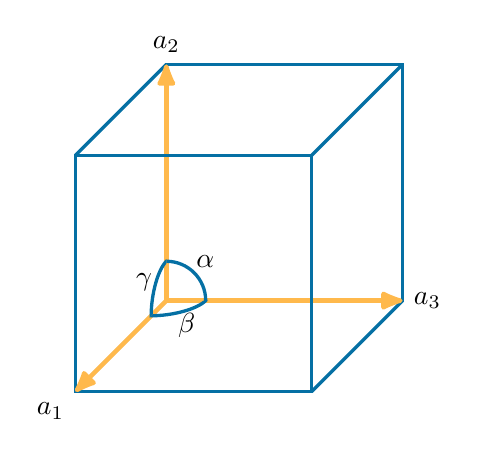
\begin{tikzpicture}
            \tikzset{edge/.style={highlight, very thick}}
            \tikzset{vector/.style={>={Latex[round]},
                    complementary, ultra thick, text=black}}
            \tikzset{angle/.style={highlight, very thick}}
            % Edges
            \draw[edge] (0, 0, 0) rectangle (3, 3, 0);
            \draw[edge] (0, 0, 3) rectangle (3, 3, 3);
            \draw[edge] (0, 0, 0) -- (0, 0, 3);
            \draw[edge] (0, 3, 0) -- (0, 3, 3);
            \draw[edge] (3, 0, 0) -- (3, 0, 3);
            \draw[edge] (3, 3, 0) -- (3, 3, 3);
            % Lattice vectors
            \draw[->, vector] (0, 0, 0) -- (0, 0, 3) node[below left] {\(\vv{a_1}\)};
            \draw[->, vector] (0, 0, 0) -- (0, 3, 0) node[above] {\(\vv{a_2}\)};
            \draw[->, vector] (0, 0, 0) -- (3, 0, 0) node[right] {\(\vv{a_3}\)};
            % Draw over lattice vectors where they cross under edges
            \draw[edge] (0, 3, 3) -- (3, 3, 3);
            \draw[edge] (3, 0, 3) -- (3, 3, 3);
            % Angles
            \begin{scope}[canvas is xy plane at z=0]
                \clip (0, 0) rectangle (1, 1);
                \draw[angle] circle [radius = 0.5];
                \node at (45:0.7) {\(\alpha\)};
            \end{scope}
            \begin{scope}[canvas is yz plane at x=0]
                \clip (0, 0) rectangle (1, 1);
                \draw[angle] circle [radius = 0.5];
                \node at (55:0.9) {\(\gamma\)};
            \end{scope}
            \begin{scope}[canvas is zx plane at y=0]
                \clip (0, 0) rectangle (1.2, 1.2);
                \draw[angle] circle [radius = 0.5];
                \node at (35:1) {\(\beta\)};
            \end{scope}
        \end{tikzpicture}
        \caption[Unit cell and lattice vectors.]{A unit cell spanned by the lattice vectors \(\vv{a_1}\), \(\vv{a_2}\), and \(\vv{a_3}\).}
        \label{fig:unit cell}
    \end{figure}
    
    The volume of the unit cell is given by the scalar triple product:
    \begin{equation}
        V = \abs{\vv{a_1}\cdot (\vv{a_2}\times\vv{a_3})}
    \end{equation}

    \subsection{Symmetries}
    We can learn a lot about a crystal from the symmetries that it possess, or fails to posses.
    We can see the symmetry of many crystals from the shapes that they form.
    For example, cubic pyrite, \ce{FeS2}, forms cubic crystals.
    These have four-fold rotational symmetry about their faces, and also three fold rotational symmetry about their points.
    There are a few types of symmetry that are interesting for crystals and we shall discus these in this section.
    
    \subsubsection{Mirror Plane Symmetry}
    A \defineindex{mirror plane symmetry} means that there is a plane (or in two dimensions a line) through which we can reflect the object and the result is identical to having done nothing.
    For example a simple square has four mirror symmetries:
    \begin{equation*}
        \tikzsetnextfilename{mirror-symmetry-square}
        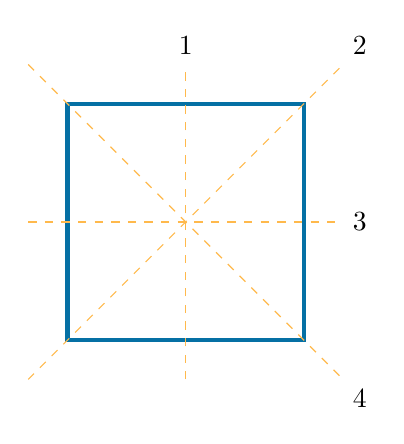
\begin{tikzpicture}
            \draw[highlight, ultra thick] (-1.5, -1.5) rectangle (1.5, 1.5);
            \draw[complementary, dashed, text=black] (0, -2) -- (0, 2) node[above] {1};
            \draw[complementary, dashed, text=black] (-2, 0) -- (2, 0) node[right] {3};
            \draw[complementary, dashed, text=black] (-2, -2) -- (2, 2) node[above right] {2};
            \draw[complementary, dashed, text=black] (-2, 2) -- (2, -2) node[below right] {4};
        \end{tikzpicture}
    \end{equation*}
    If we introduce another feature, such as dots, we reduce the number of symmetries:
    \begin{equation*}
        \tikzsetnextfilename{mirror-symmetry-dot-square}
        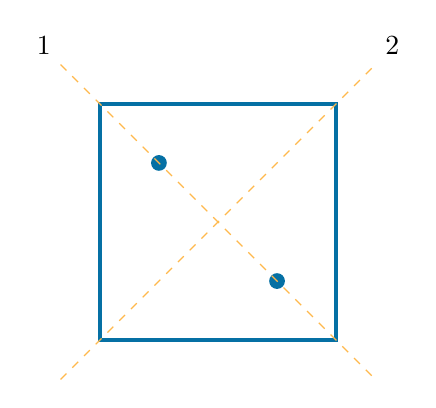
\begin{tikzpicture}
            \draw[highlight, ultra thick] (-1.5, -1.5) rectangle (1.5, 1.5);
            \fill[highlight] (-0.75, 0.75) circle [radius = 0.1];
            \fill[highlight] (0.75, -0.75) circle [radius = 0.1];
            \draw[complementary, dashed, text=black] (-2, -2) -- (2, 2) node[above right] {2};
            \draw[complementary, dashed, text=black] (-2, 2) -- (2, -2) node[above left, pos=0] {1};
        \end{tikzpicture}
    \end{equation*}
    
    A cube similarly has mirror plane symmetries, in fact, it has 9 of them. 
    This is shown in \cref{fig:mirror plane symmetry of a cube}.
    \begin{figure}
        \tikzsetnextfilename{mirror-plane-symmetry-cube}
        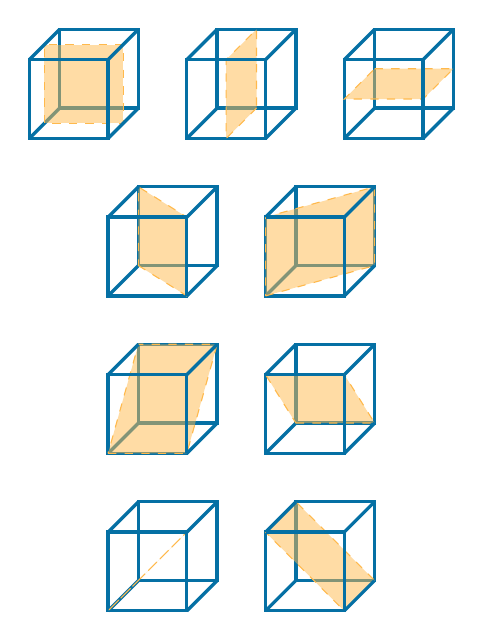
\begin{tikzpicture}
            \tikzset{edge/.style={highlight, very thick}}
            \tikzset{plane/.style={dashed, complementary, fill=complementary, fill opacity=0.5}}
            \draw[edge] (0, 0, 0) rectangle (1, 1, 0);
            \draw[edge] (0, 0, 1) rectangle (1, 1, 1);
            \draw[edge] (0, 0, 0) -- (0, 0, 1);
            \draw[canvas is xy plane at z=0.5, plane] (0, 0) rectangle (1, 1);
            \draw[edge] (0, 1, 0) -- (0, 1, 1);
            \draw[edge] (1, 0, 0) -- (1, 0, 1);
            \draw[edge] (1, 1, 0) -- (1, 1, 1);
            \draw[edge] (0, 1, 1) -- (1, 1, 1);
            \draw[edge] (1, 0, 1) -- (1, 1, 1);
            \begin{scope}[xshift=2cm]
                \draw[edge] (0, 0, 0) rectangle (1, 1, 0);
                \draw[edge] (0, 0, 1) rectangle (1, 1, 1);
                \draw[edge] (0, 0, 0) -- (0, 0, 1);
                \draw[canvas is yz plane at x=0.5, plane] (0, 0) rectangle (1, 1);
                \draw[edge] (0, 1, 0) -- (0, 1, 1);
                \draw[edge] (1, 0, 0) -- (1, 0, 1);
                \draw[edge] (1, 1, 0) -- (1, 1, 1);
                \draw[edge] (0, 1, 1) -- (1, 1, 1);
                \draw[edge] (1, 0, 1) -- (1, 1, 1);
            \end{scope}
            \begin{scope}[xshift=4cm]
                \draw[edge] (0, 0, 0) rectangle (1, 1, 0);
                \draw[edge] (0, 0, 1) rectangle (1, 1, 1);
                \draw[edge] (0, 0, 0) -- (0, 0, 1);
                \draw[canvas is zx plane at y=0.5, plane] (0, 0) rectangle (1, 1);
                \draw[edge] (0, 1, 0) -- (0, 1, 1);
                \draw[edge] (1, 0, 0) -- (1, 0, 1);
                \draw[edge] (1, 1, 0) -- (1, 1, 1);
                \draw[edge] (0, 1, 1) -- (1, 1, 1);
                \draw[edge] (1, 0, 1) -- (1, 1, 1);
            \end{scope}
            \begin{scope}[yshift=-2cm, xshift=1cm]
                \draw[edge] (0, 0, 0) rectangle (1, 1, 0);
                \draw[edge] (0, 0, 1) rectangle (1, 1, 1);
                \draw[edge] (0, 0, 0) -- (0, 0, 1);
                \draw[plane] (0, 0, 0) -- (1, 0, 1) -- (1, 1, 1) -- (0, 1, 0) -- cycle;
                \draw[edge] (0, 1, 0) -- (0, 1, 1);
                \draw[edge] (1, 0, 0) -- (1, 0, 1);
                \draw[edge] (1, 1, 0) -- (1, 1, 1);
                \draw[edge] (0, 1, 1) -- (1, 1, 1);
                \draw[edge] (1, 0, 1) -- (1, 1, 1);
            \end{scope}
            \begin{scope}[yshift=-2cm, xshift=3cm]
                \draw[edge] (0, 0, 0) rectangle (1, 1, 0);
                \draw[edge] (0, 0, 1) rectangle (1, 1, 1);
                \draw[edge] (0, 0, 0) -- (0, 0, 1);
                \draw[plane] (0, 0, 1) -- (1, 0, 0) -- (1, 1, 0) -- (0, 1, 1) -- cycle;
                \draw[edge] (0, 1, 0) -- (0, 1, 1);
                \draw[edge] (1, 0, 0) -- (1, 0, 1);
                \draw[edge] (1, 1, 0) -- (1, 1, 1);
                \draw[edge] (0, 1, 1) -- (1, 1, 1);
                \draw[edge] (1, 0, 1) -- (1, 1, 1);
            \end{scope}
            \begin{scope}[yshift=-4cm, xshift=1cm]
                \draw[edge] (0, 0, 0) rectangle (1, 1, 0);
                \draw[edge] (0, 0, 1) rectangle (1, 1, 1);
                \draw[edge] (0, 0, 0) -- (0, 0, 1);
                \draw[plane] (0, 0, 1) -- (1, 0, 1) -- (1, 1, 0) -- (0, 1, 0) -- cycle;
                \draw[edge] (0, 1, 0) -- (0, 1, 1);
                \draw[edge] (1, 0, 0) -- (1, 0, 1);
                \draw[edge] (1, 1, 0) -- (1, 1, 1);
                \draw[edge] (0, 1, 1) -- (1, 1, 1);
                \draw[edge] (1, 0, 1) -- (1, 1, 1);
            \end{scope}
            \begin{scope}[yshift=-4cm, xshift=3cm]
                \draw[edge] (0, 0, 0) rectangle (1, 1, 0);
                \draw[edge] (0, 0, 1) rectangle (1, 1, 1);
                \draw[edge] (0, 0, 0) -- (0, 0, 1);
                \draw[plane] (0, 0, 0) -- (1, 0, 0) -- (1, 1, 1) -- (0, 1, 1) -- cycle;
                \draw[edge] (0, 1, 0) -- (0, 1, 1);
                \draw[edge] (1, 0, 0) -- (1, 0, 1);
                \draw[edge] (1, 1, 0) -- (1, 1, 1);
                \draw[edge] (0, 1, 1) -- (1, 1, 1);
                \draw[edge] (1, 0, 1) -- (1, 1, 1);
            \end{scope}
            \begin{scope}[yshift=-6cm, xshift=1cm]
                \draw[edge] (0, 0, 0) rectangle (1, 1, 0);
                \draw[edge] (0, 0, 1) rectangle (1, 1, 1);
                \draw[edge] (0, 0, 0) -- (0, 0, 1);
                \draw[plane] (0, 0, 0) -- (0, 0, 1) -- (1, 1, 1) -- (1, 1, 0) -- cycle;
                \draw[edge] (0, 1, 0) -- (0, 1, 1);
                \draw[edge] (1, 0, 0) -- (1, 0, 1);
                \draw[edge] (1, 1, 0) -- (1, 1, 1);
                \draw[edge] (0, 1, 1) -- (1, 1, 1);
                \draw[edge] (1, 0, 1) -- (1, 1, 1);
            \end{scope}
            \begin{scope}[yshift=-6cm, xshift=3cm]
                \draw[edge] (0, 0, 0) rectangle (1, 1, 0);
                \draw[edge] (0, 0, 1) rectangle (1, 1, 1);
                \draw[edge] (0, 0, 0) -- (0, 0, 1);
                \draw[plane] (1, 0, 0) -- (1, 0, 1) -- (0, 1, 1) -- (0, 1, 0) -- cycle;
                \draw[edge] (0, 1, 0) -- (0, 1, 1);
                \draw[edge] (1, 0, 0) -- (1, 0, 1);
                \draw[edge] (1, 1, 0) -- (1, 1, 1);
                \draw[edge] (0, 1, 1) -- (1, 1, 1);
                \draw[edge] (1, 0, 1) -- (1, 1, 1);
            \end{scope}
        \end{tikzpicture}
        \caption[Mirror plane symmetries of a cube.]{Mirror plane symmetries of a cube, there are 9 in total.}
        \label{fig:mirror plane symmetry of a cube}
    \end{figure}
    
    \subsubsection{Rotational Symmetry}
    An object has \(k\)-fold \defineindex{rotational symmetry} about some axis, \(\vh{n}\) if it is possible to rotate the object by some multiple of \(2\pi/k\) about \(\vh{n}\) and it looks like nothing has happened.
    For example, \cref{fig:rotational symmetry star} shows a five pointed star with 5-fold rotational symmetry, including a rotation by 0 or \(2\pi\), which is equivalent to doing nothing.\footnote{The symmetry group is \(\integers_5\), or more generally for a \(k\)-fold rotationally symmetric object, \(\integers_k\).}
    
    \begin{figure}
        \tikzsetnextfilename{rotational-symmetry-star}
        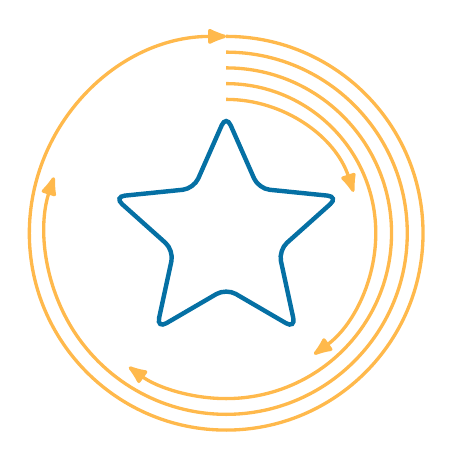
\begin{tikzpicture}
            \node[star, draw, minimum size=3cm, ultra thick, highlight, star point height=0.8cm, rounded corners] {};
            \draw[-{Latex[round]}, very thick, complementary] (90:1.7) arc (90:18:1.7);
            \draw[-{Latex[round]}, very thick, complementary] (90:1.9) arc (90:-54:1.9);
            \draw[-{Latex[round]}, very thick, complementary] (90:2.1) arc (90:-126:2.1);
            \draw[-{Latex[round]}, very thick, complementary] (90:2.3) arc (90:-198:2.3);
            \draw[-{Latex[round]}, very thick, complementary] (90:2.5) arc (90:-270:2.5);
        \end{tikzpicture}
        \caption[Five fold rotational.]{A five pointed star has 5-fold rotational symmetry, including a rotation by \(0\) or \(2\pi\), which is the identity, in that it leaves the shape completely the same.}
        \label{fig:rotational symmetry star}
    \end{figure}

    A square has four-fold rotational symmetry.\footnote{The dihedral group, \(D_4\), is the symmetry group of a square combining the rotational and reflective symmetries.}
    A cube also has rotational symmetries, but in three dimensions things are more complicated as we have far more choices of axes of rotation.
    \Cref{fig:rotational symmetry cube} shows a cube with three axes of rotational symmetry.
    The first connects two diagonally opposite corners.
    The cube has three-fold rotational symmetry about this axis.
    The second connects the mid points of two diagonally opposite edges.
    The cube has two-fold rotational symmetry about this axis.
    The third connects the centre of two opposite faces.
    The cube has four-fold rotational symmetry about this axis.
    There are four axes of the first type, six of the second type, and three of the third type, for 13 total axes of rotation.
    
    \begin{figure}
        \tikzsetnextfilename{rotational-symmetry-cube}
        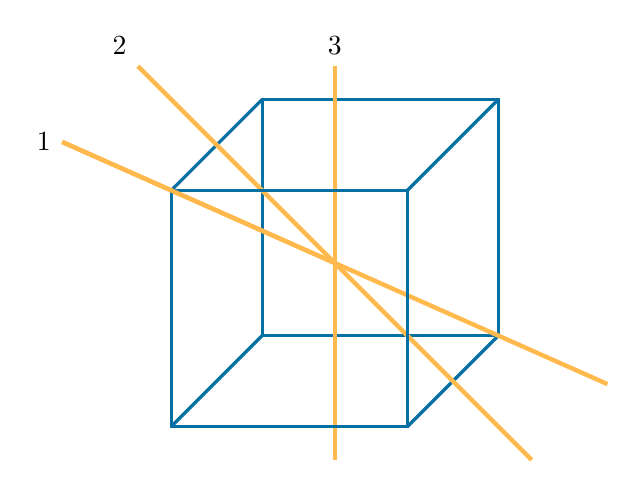
\begin{tikzpicture}
            \tikzset{edge/.style={very thick, highlight}}
            \draw[edge] (0, 0, 0) rectangle (3, 3, 0);
            \draw[edge] (0, 0, 0) -- (0, 0, 3);
            \draw[edge] (3, 3, 0) -- (3, 3, 3);
            \draw[edge] (0, 3, 0) -- (0, 3, 3);
            \draw[edge] (3, 0, 0) -- (3, 0, 3);
            \draw[edge] (2.5, 0, 0) -- (3, 0, 0) -- (3, 0.5, 0);
            \draw[ultra thick, complementary, text=black] (1.5, -1, 1.5) -- (1.5, 4, 1.5) node[above] {3};
            \draw[ultra thick, complementary, text=black] (-1, 4, 4) -- (4, -1, -1) node[left, pos=0] {1};
            \draw[ultra thick, complementary, text=black] (-1, 4, 1.5) -- (4, -1, 1.5) node[above left, pos=0] {2};
            \draw[edge] (0, 0, 3) rectangle (3, 3, 3);
            \draw[ultra thick, complementary, text=black] (-1, 4, 4) -- (1.5, 1.5, 1.5);
        \end{tikzpicture}
        \caption[Rotational symmetry of a cube]{Three possible axes of rotational symmetry of the cube.}
        \label{fig:rotational symmetry cube}
    \end{figure}
    
    \subsubsection{Inversion}
    An \defineindex{inversion symmetry} is reflection through a point, called the \defineindex{centre of inversion}, which leaves the object unchanged.
    For example, this graph,
    \begin{equation*}
        \tikzsetnextfilename{inversion-symmetry-plane}
        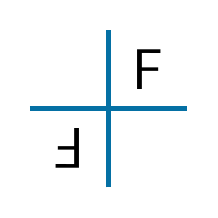
\begin{tikzpicture}
            \draw[highlight, ultra thick] (-1, 0) -- (1, 0);
            \draw[highlight, ultra thick] (0, -1) -- (0, 1);
            \node at (0.5, 0.5) {\huge\textsf{\textsf{F}}};
            \node[rotate around={180:(0,0)}] at (-0.5, -0.5) {\huge\textsf{\textsf{F}}};
        \end{tikzpicture}
    \end{equation*}
    has a centre of inversion at the origin.
    
    This tetrahedron,
    \begin{equation*}
        \tikzsetnextfilename{inversion-symmetry-tetrahedron}
        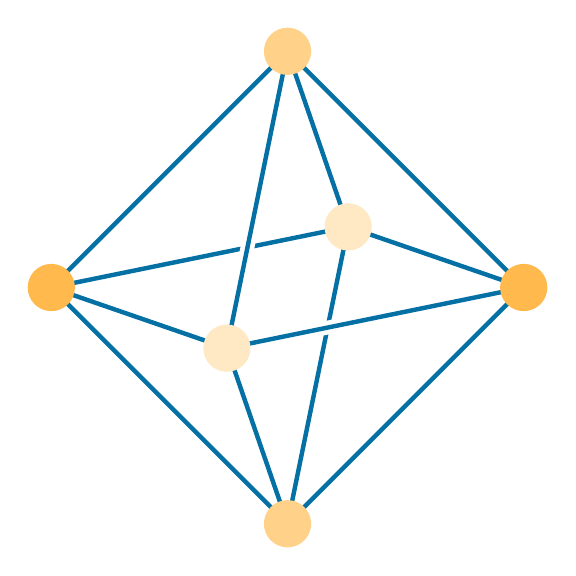
\begin{tikzpicture}
            \tikzset{edge/.style={ultra thick, highlight}}
            \tikzset{under edge/.style={line width=5pt, white}}
            \draw[edge] (3, 0, -2) -- (3, -3, 0);
            \draw[under edge] (3, 0, 2) -- (6, 0, 0);
            \draw[edge] (0, 0, 0) -- (3, 0, 2) -- (6, 0, 0) -- (3, 0, -2) -- cycle;
            \draw[edge] (0, 0, 0) -- (3, 3, 0);
            \draw[under edge] (3, 0, 2) -- (3, 3, 0);
            \draw[edge] (3, 0, 2) -- (3, 3, 0);
            \draw[edge] (6, 0, 0) -- (3, 3, 0);
            \draw[edge] (3, 0, -2) -- (3, 3, 0);
            \draw[edge] (0, 0, 0) -- (3, -3, 0);
            \draw[edge] (3, 0, 2) -- (3, -3, 0);
            \draw[edge] (6, 0, 0) -- (3, -3, 0);
            
            \fill[complementary] (0, 0, 0) circle [radius = 0.3];
            \fill[complementary] (6, 0, 0) circle [radius = 0.3];
            \fill[complementary!33] (3, 0, 2) circle [radius = 0.3];
            \fill[complementary!33] (3, 0, -2) circle [radius = 0.3];
            \fill[complementary!66] (3, 3, 0) circle [radius = 0.3];
            \fill[complementary!66] (3, -3, 0) circle [radius = 0.3];
        \end{tikzpicture}
    \end{equation*}
    has a centre of inversion at its centre.
    The corresponding symmetry swaps points of the same shade.
    
    A cube has a centre of inversion at its centre.
    Combining this with the 9 mirror plane symmetries and 13 rotational symmetries we see a cube has 24 symmetries to consider.
    
    \subsection{Symmetry Applications to Crystals}
    Suppose a crystal has four-fold rotational symmetry.
    It is not difficult to convince yourself that this can only be the case if \(\abs{\vv{a_1}} = \abs{\vv{a_2}}\) and \(\angle(\vv{a_1}, \vv{a_2}) = \pi/2\).
    We call this a square lattice for obvious reasons.
    
    If we only require two-fold rotational symmetry then we can relax the condition on the vector lengths and we get a rectangular lattice, which has \(\abs{\vv{a_1}} \ne \abs{\vv{a_2}}\) and \(\angle(\vv{a_1},\vv{a_2}) = \pi/2\).
    
    The symmetry imposes conditions on the lattice parameters.
    Similarly if a crystal has three-fold rotational symmetry then this necessitates that \(\abs{\vv{a_1}} = \abs{\vv{a_2}}\) and \(\angle(\vv{a_1}, \vv{a_2}) = 2\pi/3\).
    We call this a hexagonal lattice as three unit cells together form a regular hexagon.
    
    These three lattices, along with relevant unit cells, are shown in \cref{fig:square rectangle hexagon lattice}, as well as the three unit cells forming a hexagon in the hexagonal lattice.
    
    \begin{figure}
        \tikzsetnextfilename{square-rectangle-hexagon-lattice}
        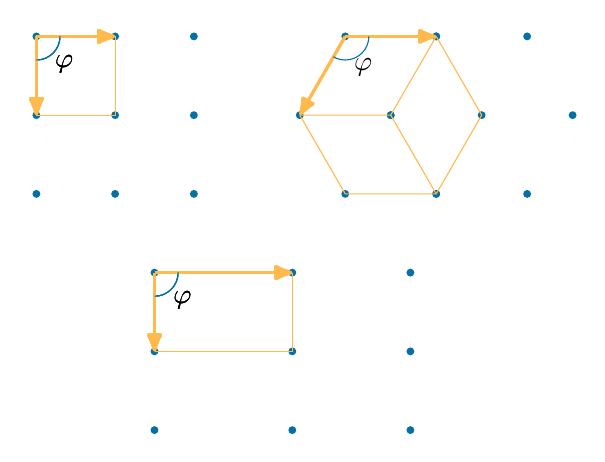
\begin{tikzpicture}
            \foreach \x in {0,..., 2} {
                \foreach \y in {0,..., 2} {
                    \fill[highlight] (\x, \y) circle [radius = 0.05];
                }
                \draw[very thick, complementary, -{Latex[round]}] (0, 2) -- (1, 2);
                \draw[very thick, complementary, -{Latex[round]}] (0, 2) -- (0, 1);
                \draw[complementary] (0, 1) -- (1, 1) -- (1, 2);
                \begin{scope}
                    \clip (0, 2) rectangle (1, 1);
                    \draw[highlight] (0, 2) circle [radius = 0.3];
                \end{scope}
                \node at ($(0, 2) + (-45:0.5)$) {\(\varphi\)};
            }
            \begin{scope}[xshift=3.5cm]
                \fill[highlight] (1, 1) circle [radius = 0.05];
                \foreach \a in {0, 60,..., 300} {
                    \fill[highlight] ($(1, 1) + (\a:1.155)$) circle [radius = 0.05];
                    \fill[highlight] ($(1, 1) + (\a:1.155) + (0:1.155)$) circle [radius = 0.05];
                }
                \draw[very thick, complementary, -{Latex[round]}] ($(1, 1) + (120:1.155)$) -- ($(1, 1) + (60:1.155)$);
                \draw[very thick, complementary, -{Latex[round]}] ($(1, 1) + (120:1.155)$) -- ($(1, 1) + (180:1.155)$);
                \draw[complementary] ($(1, 1) + (180:1.155)$) -- ($(1, 1) + (240:1.155)$) -- ($(1, 1) + (300:1.155)$) -- ($(1, 1) + (0:1.155)$) -- ($(1, 1) + (60:1.155)$);
                \draw [complementary] ($(1, 1) + (180:1.155)$) -- (1, 1) -- ($(1, 1) + (-60:1.155)$);
                \draw [complementary] (1, 1) -- ($(1, 1) + (60:1.155)$);
                \begin{scope}
                    \clip ($(1, 1) + (120:1.155)$) -- ($(1, 1) + (60:1.155)$) -- (1, 1) -- ($(1, 1) + (180:1.155)$) -- cycle;
                    \draw[highlight] ($(1, 1) + (120:1.155)$) circle [radius = 0.3];
                    \node at ($(1, 1) + (120:0.70)$) {\(\varphi\)};
                \end{scope}
            \end{scope}
            \begin{scope}[xshift=1.5cm, yshift=-3cm]
                \foreach \x in {0, 1.75, 3.25} {
                    \foreach \y in {0,..., 2} {
                        \fill[highlight] (\x, \y) circle [radius = 0.05];
                    }
                    \draw[very thick, complementary, -{Latex[round]}] (0, 2) -- (1.75, 2);
                    \draw[very thick, complementary, -{Latex[round]}] (0, 2) -- (0, 1);
                    \draw[complementary] (0, 1) -- (1.75, 1) -- (1.75, 2);
                    \begin{scope}
                        \clip (0, 2) rectangle (1.75, 1);
                        \draw[highlight] (0, 2) circle [radius = 0.3];
                    \end{scope}
                    \node at ($(0, 2) + (-45:0.5)$) {\(\varphi\)};
                }
            \end{scope}
        \end{tikzpicture}
        \caption[Square, rectangular, and hexagonal lattice vectors in 2D]{A square lattice (top left), hexagonal lattice (top right), and hexagonal lattice (bottom). For the square and rectangular lattices \(\varphi = \pi/2\) and for the hexagonal lattice \(\varphi = 2\pi/3\). For the square and hexagonal lattice \(\abs{\vv{a_1}} = \abs{\vv{a_2}}\).}
        \label{fig:square rectangle hexagon lattice}
    \end{figure}
    
    What we are discussing are two-dimensional lattices.
    The three we have discussed are the result of symmetry restrictions.
    There is also a lattice that results from no symmetry restrictions, called the centred rectangular lattice.
    This is shown in \cref{fig:centred rectangular lattice}.
    The primitive unit cell shown is awkward to work with and doesn't lead to much insight.
    If we allow ourselves to work with non-primitive unit cells then the second unit cell shown is a more sensible choice.
    This is called a centred rectangular unit cell, since it is rectangular and has a lattice point at its centre.
    
    \begin{figure}
        \tikzsetnextfilename{centred-rectangular-lattice}
        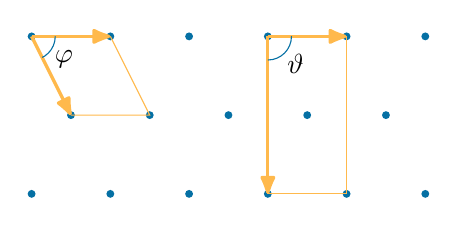
\begin{tikzpicture}
            \foreach \x in {0,...,4} {
                \fill[highlight] (\x + 1, 0) circle [radius = 0.05];
                \fill[highlight] (\x + 0.5, 1) circle [radius = 0.05];
                \fill[highlight] (\x, 2) circle [radius = 0.05];
            }
            \fill[highlight] (0, 0) circle [radius = 0.05];
            \fill[highlight] (5, 2) circle [radius = 0.05];
            \draw[very thick, complementary, -{Latex[round]}] (0, 2) -- (1, 2);
            \draw[very thick, complementary, -{Latex[round]}] (0, 2) -- (0.5, 1);
            \draw[complementary] (0.5, 1) -- (1.5, 1) -- (1, 2);
            \begin{scope}
                \clip (0, 2) -- (1, 2) -- (1.5, 1) -- (0.5, 1) -- cycle;
                \draw[highlight] (0, 2) circle [radius = 0.3];
            \end{scope}
            \node at ($(0, 2) + (-35:0.5)$) {\(\varphi\)};
            \draw[very thick, complementary, -{Latex[round]}] (3, 2) -- (3, 0);
            \draw[very thick, complementary, -{Latex[round]}] (3, 2) -- (4, 2);
            \draw[complementary] (3, 2) rectangle (4, 0);
            \begin{scope}
                \clip (3, 2) rectangle (4, 0);
                \draw[highlight] (3, 2) circle [radius = 0.3];
            \end{scope}
            \node at ($(3, 2) + (-45:0.5)$) {\(\vartheta\)};
        \end{tikzpicture}
        \caption[Primitive and standard centred rectangular lattice.]{The centred rectangular lattice with its primitive unit cell and the simpler choice of a centred rectangular unit cell.}
        \label{fig:centred rectangular lattice}
    \end{figure}
    
    The four two-dimensional lattices we have seen cover all possible cases.
    These are together known as the two-dimensional \defineindex{Bravais lattices}.
    They are summarised in \cref{tab:2d bravais lattices}.
    
    \begin{table}
        \caption[2D Bravais lattices.]{The key information about two-dimensional Bravais lattices.}
        \label{tab:2d bravais lattices}
        \begin{tabular}{lll}
            \toprule
            Crystal & External Minimum Symmetry & Restrictions\\ \midrule
            \multirow{2}{*}{Square} & \multirow{2}{*}{Four-fold rotational symmetry} & \(\abs{\vv{a_1}} = \abs{\vv{a_2}}\)\\
            && \(\angle(\vv{a_1},\vv{a_2}) = \pi/2\)\\\midrule
            Rectangular & Two-fold rotational symmetry & \(\angle(\vv{a_1},\vv{a_2}) = \pi/2\)\\\midrule
            \multirow{2}{*}{Hexagonal} & \multirow{2}{*}{Three-fold rotational symmetry} & \(\abs{\vv{a_1}} = \abs{\vv{a_2}}\)\\
            && \(\angle(\vv{a_1},\vv{a_2}) = 2\pi/3\)\\
            Centred Rectangular & None & None\\
            \bottomrule
        \end{tabular}
    \end{table}
    
    In three dimensions we can make similar arguments about symmetries and the resulting restrictions on the lattice parameters.
    We end up with a list of seven three-dimensional Bravais lattices.
    The key information for these is in \cref{tab:3d bravais lattices}.
    
    \begin{table}
        \caption[3D Bravais lattices.]{The key information about three-dimensional Bravais lattices.}
        \label{tab:3d bravais lattices}
        \begin{tabular}{lll}\toprule
            Crystal & External Minimum Symmetry & Restrictions\\\midrule
            \multirow{2}{*}{Cubic} & \multirow{2}{*}{\parbox{4.4cm}{Four three-fold rotational symmetries}} & \(a = b = c\)\\
            && \(\alpha = \beta = \gamma = \pi/2\)\\\midrule
            \multirow{2}{*}{Hexagonal} & \multirow{2}{*}{\parbox{4.3cm}{One six-fold rotational symmetry}} & \(a = b\), \(\gamma = 2\pi/3\)\\
            && \(\alpha = \beta = \pi/2\)\\\midrule
            \multirow{3}{*}{Trigonal} & \multirow{3}{*}{\parbox{4.4cm}{One three-fold rotational symmetry}} & \(a = b = c\)\\
            && \(\alpha = \beta = \gamma \le 2\pi/3\)\\
            && \(\alpha \ne \pi/2\)\\\midrule
            \multirow{2}{*}{Tetragonal} & \multirow{2}{*}{\parbox{4.4cm}{One four-fold rotational symmetry}} & \(a = b\)\\
            && \(\alpha = \beta = \gamma = \pi/2\)\\\midrule
            Orthorhombic & \parbox{4.4cm}{Three perpendicular two-fold rotational symmetries} & \(\alpha = \beta = \gamma = \pi/2\)\\\midrule
            Monoclinic & \parbox{4.4cm}{One two-fold rotational symmetry, parallel to \(b\)} & \(\alpha = \gamma = \pi/2 \ne \beta\)\\\midrule
            Triclinic & None & None\\\bottomrule
        \end{tabular}
    \end{table}
    
    This isn't quite the complete picture however as we have assumed these are all primitive unit cells.
    In three dimensions there are actually four centrings, where we add additional lattice points to the unit cell, to consider.
    The first, and simplest, is the primitive unit cell, P.
    The second is face centring, F, where we add an extra lattice point to every face.
    The third is body centring, I, where we add an extra lattice point to the centre of the cell (I for interior).
    The fourth is base centred, denoted either A, B, or C, where we add an extra lattice point to one pair of opposite faces.
    If we add to the face spanned by \(\vv{a_1}\) and \(\vv{a_2}\) then we call it C, the face spanned by \(\vv{a_1}\) and \(\vv{a_3}\) corresponds to B, and the face spanned by \(\vv{a_2}\) and \(\vv{a_3}\) corresponds to A.
    Not all crystal system and centring pairings give us a useful lattice however.
    The ones that do are given in \cref{tab:crystal system centring}.
    We are now in a position to fully specify a crystal lattice by stating the crystal structure and the centring.
    \begin{table}
        \caption[Crystal structure centrings.]{Crystal systems and centrings. Note that R stands for rhombohedral, a trigonal crystal can be categorised as having either a hexagonal or rhombohedral lattice system}
        \label{tab:crystal system centring}
        \begin{tabular}{ll}\toprule
            Crystal System & Centring\\\midrule
            Cubic & P, F, and I\\
            Hexagonal & P\\
            Trigonal & P, and R\\
            Tetragonal & P, and I\\
            Orthorhombic & P, I, and F\\
            Monoclinic & P, and A/B/C\\
            Triclinic & P\\\bottomrule
        \end{tabular}
    \end{table}

    \subsection{Basis}
    Now that we can fully specify a crystal lattice we need to use this to define a crystal.
    We do this with the help of a basis, which is a list of atoms and locations that they occur in the unit cell.
    We typically give these locations in dimensionless, reduced coordinates, \((x, y, z)\), corresponding to the position
    \begin{equation}
        \vv{r} = x\vv{a_1} + y\vv{a_2} + z\vv{a_3}
    \end{equation}
    The simplest basis is to have only a single atom at \(\vv{r} = (0, 0, 0)\).
    This is the case with many pure metals, for example \ce{Na}, \ce{Ba}, and \ce{Fe} all have body-centred cubic lattices (BCC)\glossary[acronym]{BCC}{body-centred cubic} with this basis, and \ce{Ca}, \ce{Ni}, and \ce{Au} have face-centred cubic lattices (FCC)\glossary[acronym]{FCC}{face-centred cubic} with this basis.
    It is worth looking at these examples in more detail.
    
    \subsubsection{Body-Centred Cubic}
    A body-centred cubic lattice unit cell consists of lattice points at the eight corners of a cube, and one lattice point in the middle.
    We consider the case of the basis being a single atom at \((0, 0, 0)\).
    The conventional lattice vectors in this case are \(\vv{a_1} = a\vh{x}\), \(\vv{a_2} = a\vh{y}\), and \(\vv{a_3} = a\vh{z}\), where \(\vh{x}\), \(\vh{y}\), and \(\vh{z}\) are orthonormal Cartesian unit vectors.
    There are two atoms in the conventional unit cell, one at the centre, and 1/8 of an atom in each corner, these are shared between the neighbouring cells.
    The positions of the atoms in reduced coordinates in the unit cell are \((0, 0, 0)\) and \((1/2, 1/2, 1/2)\).
    Each atom has 8 nearest neighbours and 6 next-nearest neighbours.
    
    The primitive unit cell is more complicated so we don't use it often but it has lattice vectors
    \begin{equation}
        \vv{a_1^P} = \frac{a}{2}(-\vh{x} + \vh{y} + \vh{z}), \qquad \vv{a_2^P} = \frac{a}{2}(\vh{x} - \vh{y} + \vh{z}), \qqand \vv{a_3^P} = \frac{a}{2}(\vh{x} + \vh{y} - \vh{z}).
    \end{equation}
    It is clear why one would prefer a centred cubic lattice over this oddly shaped primitive lattice.
    
    \begin{figure}
        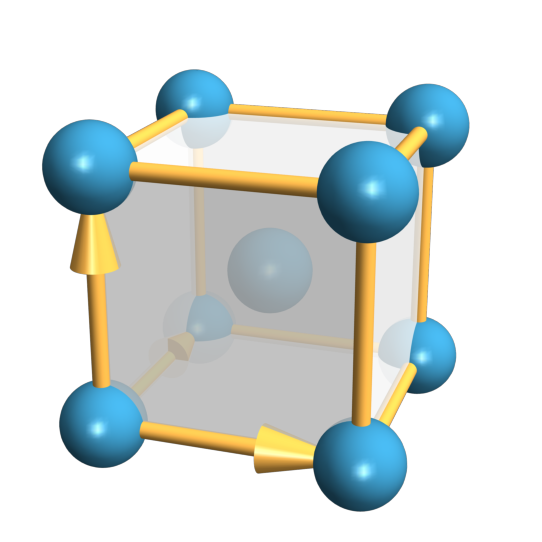
\includegraphics{images/bcc-crystal.pdf}
        \caption[BCC crystal]{A body-centred crystal.}
    \end{figure}
    
    \subsubsection{Face-Centred Cubic}
    A face-centred cubic lattice unit cell consists of a lattice point at the eight corners of a cube, and one lattice point in the centre of each face.
    We consider the case of a basis of a single atom at \((0, 0, 0)\).
    The conventional lattice vectors in this case are \(\vv{a_1} = a\vh{x}\), \(\vv{a_2} = a\vh{y}\), and \(\vv{a_3} = a\vh{z}\), where \(\vh{x}\), \(\vh{y}\), and \(\vh{z}\) are orthonormal Cartesian unit vectors.
    There are four atoms in the conventional unit cell.
    Each of the six faces contributes half an atom, and the four corners contribute 1/8 of an atom.
    The positions of the atoms in reduced coordinates are \((0, 0, 0)\) and \((1/2, 0, 0)\).
    Each atom has 12 nearest neighbours.
    
    The primitive unit cell is more complicated so we don't use it often but it has lattice vectors
    \begin{equation}
        \vv{a_1^P} = \frac{a}{2}(\vh{y} + \vh{z}), \qquad \vv{a_2^P} = \frac{a}{2}(\vh{x} + \vh{z}), \qqand \vv{a_3^P} = \frac{a}{2}(\vh{x} + \vh{y}).
    \end{equation}
    It is clear why one would prefer a centred cubic lattice over this oddly shaped primitive lattice.
    
    The face-centred cubic lattice is the densest possible way to pack hard, non-overlapping spheres.
    For this reason it is also called \defineindex{cubic close packed} (CCP)\glossary[acronym]{CCP}{cubic close-packed}.
    
    \begin{figure}
        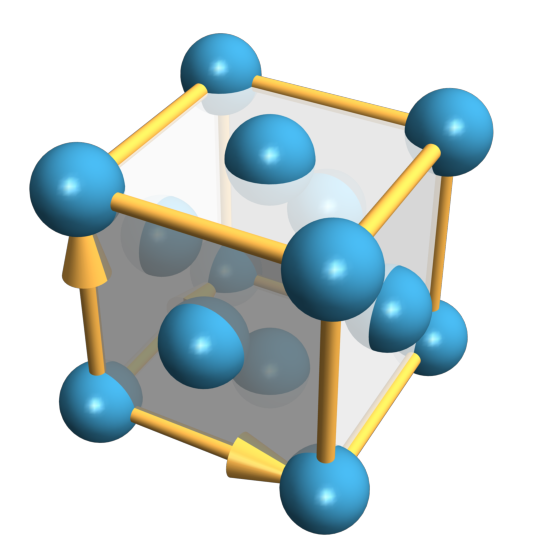
\includegraphics{images/fcc-crystal.pdf}
        \caption[FCC crystal.]{A face-centred crystal.}
    \end{figure}
    
    \subsubsection{Hexagonal Close-Packed}
    A hexagonal close-packed (HCP)\glossary[acronym]{HCP}{hexagonal close-packed} consists of a hexagonal unit cell, with lattice parameters \(a = b\) and \(\gamma = 2\pi/3\).
    There are two atoms in the conventional unit cell, positioned at \((2/3,1/3,1/4)\) and \((1/3,2/3,3/4)\).
    Each atom has 12 nearest neighbours.
    The packing density of this structure is equal to that of cubic close-packing.
    There is no conventional choice of lattice vectors, but one option is
    \begin{equation}
        \vv{a_1} = a\frac{\sqrt{3}}{2}\vh{x} + \frac{a}{2}\vh{y}, \qquad \vv{a_2} = -a\frac{\sqrt{3}}{2}\vh{x} + \frac{a}{2}\vh{y}, \qqand \vv{a_3} = c\vh{z}.
    \end{equation}

    \subsubsection{Close Packing}
    Both cubic and hexagonal close packing can be created by layering hexagonally arranged layers of spheres.
    The difference comes in where you choose to place the third layer.
    If you choose to place the third layer such that it lines up with the first layer then the result will be hexagonal close packing.
    If you choose instead to place it so that it doesn't line up you will get cubic close-packing.
    
    \subsubsection{Real Life Example}
    Consider \ce{NaCl}, common table salt, this has a face-centred cubic lattice.
    We need to choose an atom type to have at the position \((0, 0, 0)\), we arbitrarily choose \ce{Cl}.
    The basis is then a \ce{Cl} atom at \((0, 0, 0)\) and a \ce{Na} atom at \((1/2,0,0)\), or equivalently at \((1/2,1/2,1/2)\).
    
    Crystals can become very complicated in the real world but they can always be broken down into a choice of lattice and centring and a basis of atoms.
    
    \chapter{Crystal Planes}
    \section{What Are They, and Why Do We Care?}
    Crystal planes are sets of parallel planes upon which all of the atoms in a crystal can be located.
    The nature of the planes in a crystal can be important for its physical properties.
    The most obvious example being diffraction, and in particular Bragg's law, which predicts from the spacing between parallel planes what diffraction pattern will occur.
    We will see this later when we consider diffraction in more detail.
    
    Transport properties (such as conductivity, both thermal and electrical) are also dependent on planes.
    Some materials have anisotropic transport properties, that is they may be better at transport in one direction.
    For example, graphite is made of layers of planes in which the atoms are arranged hexagonally.
    Graphite is a much better as an electrical and thermal conductor along the planes rather than across the planes.
    
    Planes can also be important for the for structural properties of materials.
    A crystal is much more likely to break along a plane and plastic deformation, such as a metal being permanently bent, most often occurs when planes slip past each other.
    
    The crystal planes also effect the surface properties of a crystal.
    For example, they may effect the ability of the crystal to act as a catalyst or semiconductor.
    
    \section{Describing Planes}
    \defineindex{Miller indices} provide a standard method of naming planes.
    The naming scheme goes as follows.
    First, find where the plane intersects each axis in reduced units, say, at \((3, 2, 2)\).
    If there is no intercept then we say the intercept occurs at \(\infty\), and we take \(1/\infty = 0\).
    Second, take the reciprocals, so for our example, \((1/3, 1/2, 1/2)\).
    Third, multiply through by the smallest integer that leaves all whole numbers, in our case this is six and we get \(\crystalplane{2}{3}{3}\).
    This is the name of our plane.
    If there is a negative number then we denote this with a bar above of the number.
    
    The crystal plane \(\crystalplane{h}{k}{\ell}\) intercepts the real space axes at \(\vv{a_1}/h\), \(\vv{a_2}/k\), and \(\vv{a_3}/\ell\).
    
    The Miller indices don't represent a single plane but an infinite family of parallel planes.
    
    We can also use Miller indices to denote a direction in a crystal.
    We denote by \(\crystaldirection{h}{k}{\ell}\) the direction \(h\vv{a_1} + k\vv{a_2} + \ell\vv{a_3}\).
    In cubic, tetragonal, and orthorhombic lattices, where all angles are \(\pi/2\), the direction \(\crystaldirection{h}{k}{\ell}\) is simply the direction perpendicular to the plane \(\crystalplane{h}{k}{\ell}\).
    
    \begin{figure}
        \tikzsetnextfilename{crystal-planes}
        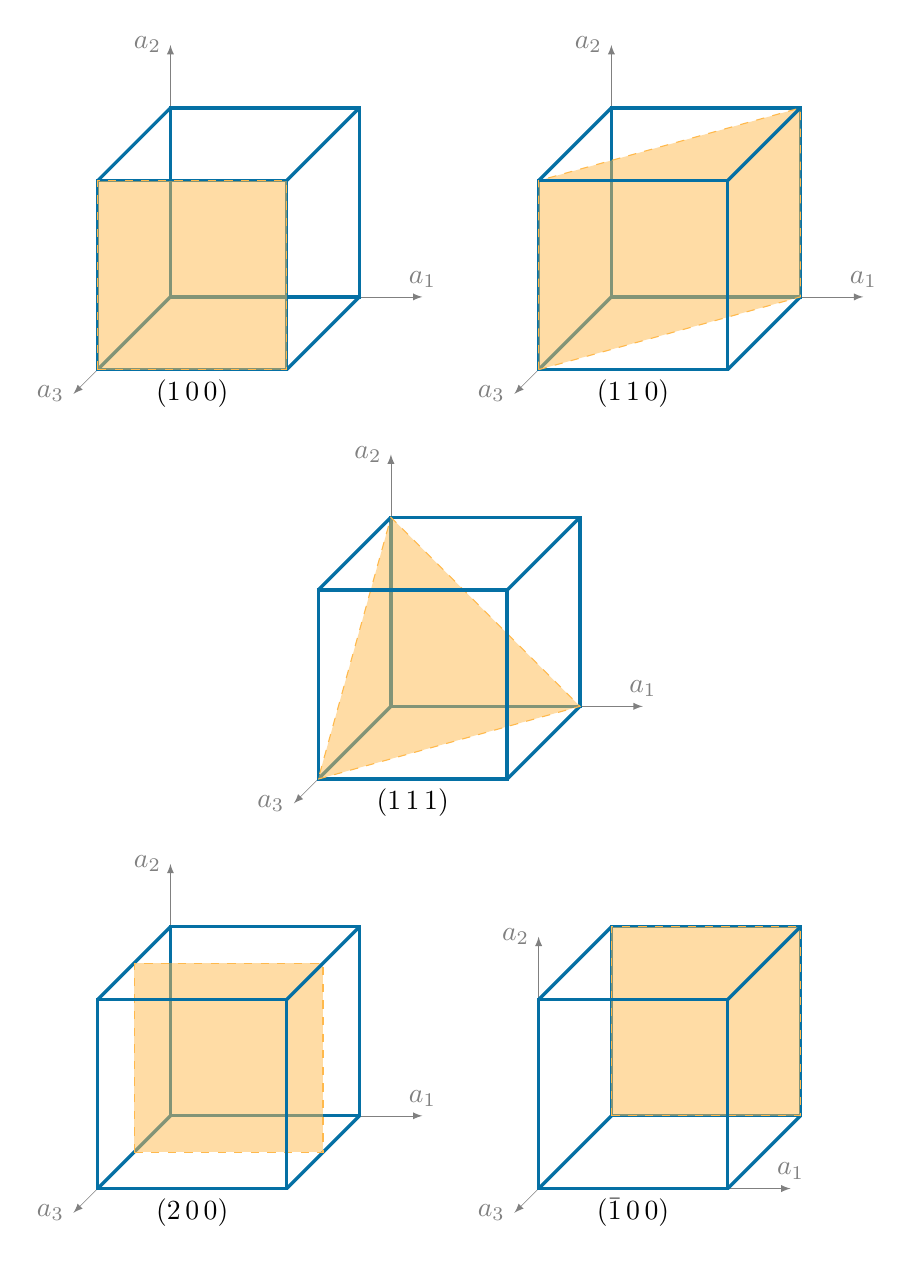
\begin{tikzpicture}[scale=0.8]
            \tikzset{edge/.style = {highlight, very thick}}
            \tikzset{plane/.style={dashed, complementary, fill=complementary, fill opacity=0.5}}
            \tikzset{axis/.style={help lines, ->}}
            \draw[axis] (0, 0, 0) -- (4, 0, 0) node[above] {\(\vv{a_1}\)};
            \draw[axis] (0, 0, 0) -- (0, 4, 0) node[left] {\(\vv{a_2}\)};
            \draw[axis] (0, 0, 0) -- (0, 0, 4) node[left] {\(\vv{a_3}\)};
            \draw[edge] (0, 0, 0) rectangle (3, 3, 0);
            \draw[edge] (0, 0, 3) rectangle (3, 3, 3);
            \draw[edge] (0, 0, 0) -- (0, 0, 3);
            \draw[edge] (0, 3, 0) -- (0, 3, 3);
            \draw[edge] (3, 0, 0) -- (3, 0, 3);
            \draw[edge] (3, 3, 0) -- (3, 3, 3);
            \draw[plane] (0, 0, 3) rectangle (3, 3, 3);
            \node[below] at (1.5, 0, 3) {\(\crystalplane{1}{0}{0}\)};
            \begin{scope}[xshift=7cm]
                \draw[axis] (0, 0, 0) -- (4, 0, 0) node[above] {\(\vv{a_1}\)};
                \draw[axis] (0, 0, 0) -- (0, 4, 0) node[left] {\(\vv{a_2}\)};
                \draw[axis] (0, 0, 0) -- (0, 0, 4) node[left] {\(\vv{a_3}\)};
                \draw[edge] (0, 0, 0) rectangle (3, 3, 0);
                \draw[edge] (0, 0, 3) rectangle (3, 3, 3);
                \draw[edge] (0, 0, 0) -- (0, 0, 3);
                \draw[edge] (0, 3, 0) -- (0, 3, 3);
                \draw[edge] (3, 0, 0) -- (3, 0, 3);
                \draw[plane] (0, 0, 3) -- (3, 0, 0) -- (3, 3, 0) -- (0, 3, 3) -- cycle;
                \draw[edge] (3, 3, 0) -- (3, 3, 3);
                \draw[edge] (0, 3, 3) -- (3, 3, 3);
                \draw[edge] (3, 0, 3) -- (3, 3, 3);
                \node[below] at (1.5, 0, 3) {\(\crystalplane{1}{1}{0}\)};
            \end{scope}
            \begin{scope}[xshift=3.5cm, yshift=-6.5cm]
                \draw[axis] (0, 0, 0) -- (4, 0, 0) node[above] {\(\vv{a_1}\)};
                \draw[axis] (0, 0, 0) -- (0, 4, 0) node[left] {\(\vv{a_2}\)};
                \draw[axis] (0, 0, 0) -- (0, 0, 4) node[left] {\(\vv{a_3}\)};
                \draw[edge] (0, 0, 0) rectangle (3, 3, 0);
                \draw[edge] (0, 0, 3) rectangle (3, 3, 3);
                \draw[edge] (0, 0, 0) -- (0, 0, 3);
                \draw[edge] (0, 3, 0) -- (0, 3, 3);
                \draw[edge] (3, 0, 0) -- (3, 0, 3);
                \draw[edge] (3, 3, 0) -- (3, 3, 3);
                \draw[plane] (0, 0, 3) -- (3, 0, 0) -- (0, 3, 0) -- cycle;
                \node[below] at (1.5, 0, 3) {\(\crystalplane{1}{1}{1}\)};
                \draw[edge] (0, 3, 3) -- (3, 3, 3);
                \draw[edge] (3, 0, 3) -- (3, 3, 3);
            \end{scope}
            \begin{scope}[yshift=-13cm]
                \draw[axis] (0, 0, 0) -- (4, 0, 0) node[above] {\(\vv{a_1}\)};
                \draw[axis] (0, 0, 0) -- (0, 4, 0) node[left] {\(\vv{a_2}\)};
                \draw[axis] (0, 0, 0) -- (0, 0, 4) node[left] {\(\vv{a_3}\)};
                \draw[edge] (0, 0, 0) rectangle (3, 3, 0);
                \draw[edge] (0, 0, 3) rectangle (3, 3, 3);
                \draw[edge] (0, 0, 0) -- (0, 0, 3);
                \draw[edge] (0, 3, 0) -- (0, 3, 3);
                \draw[edge] (3, 0, 0) -- (3, 0, 3);
                \draw[plane] (0, 0, 1.5) rectangle (3, 3, 1.5);
                \node[below] at (1.5, 0, 3) {\(\crystalplane{2}{0}{0}\)};
                \draw[edge] (0, 3, 3) -- (3, 3, 3);
                \draw[edge] (3, 0, 3) -- (3, 3, 3);
                \draw[edge] (3, 3, 0) -- (3, 3, 3);
            \end{scope}
            \begin{scope}[yshift=-13cm, xshift=7cm]
                \draw[axis] (0, 0, 3) -- (4, 0, 3) node[above] {\(\vv{a_1}\)};
                \draw[axis] (0, 0, 3) -- (0, 4, 3) node[left] {\(\vv{a_2}\)};
                \draw[axis] (0, 0, 0) -- (0, 0, 4) node[left] {\(\vv{a_3}\)};
                \draw[edge] (0, 0, 0) rectangle (3, 3, 0);
                \draw[edge] (0, 0, 3) rectangle (3, 3, 3);
                \draw[edge] (0, 0, 0) -- (0, 0, 3);
                \draw[edge] (0, 3, 0) -- (0, 3, 3);
                \draw[edge] (3, 0, 0) -- (3, 0, 3);
                \draw[plane] (0, 0, 0) rectangle (3, 3, 0);
                \node[below] at (1.5, 0, 3) {\(\crystalplane{\bar{1}}{0}{0}\)};
                \draw[edge] (0, 3, 3) -- (3, 3, 3);
                \draw[edge] (3, 0, 3) -- (3, 3, 3);
                \draw[edge] (3, 3, 0) -- (3, 3, 3);
            \end{scope}
        \end{tikzpicture}
        \caption[Crystal planes examples.]{Some crystal planes labelled by their Miller indices. Note that \(\crystalplane{1}{0}{0}\), \(\crystalplane{2}{0}{0}\), and \(\crystalplane{\bar{1}}{0}{0}\) are all parallel. The family of planes described by \(\crystalplane{1}{0}{0}\) and \(\crystalplane{\bar{1}}{0}{0}\) are the same and \(\crystalplane{2}{0}{0}\) describes these planes but also the planes directly between.}
        \label{fig:crystal planes miller indices}
    \end{figure}
    
    Consider the planes shown in \cref{fig:crystal planes miller indices}.
    In particular \(\crystalplane{1}{0}{0}\), \(\crystalplane{2}{0}{0}\), and \(\crystalplane{\bar{1}}{0}{0}\).
    Notice that \(\crystalplane{1}{0}{0}\) and \(\crystalplane{\bar{1}}{0}{0}\) describe the same set of planes.
    That is planes perpendicular to \(\vv{a_1}\) and spaced a distance \(a\) apart.
    This is because these examples are for a cubic lattice and the high symmetry means lots of planes have multiple descriptions.
    
    The planes \(\crystalplane{2}{0}{0}\) are also parallel to \(\vv{a_1}\) but they are spaced \(a/2\) apart.
    This means that the family of planes \(\crystalplane{2}{0}{0}\) contains all the planes described by \(\crystalplane{1}{0}{0}\), and also all of the planes halfway between.
    
    \chapter{Diffraction}
    \section{Experimental Setup}
    Crystal \defineindex{diffraction} is most often done with x-rays, although it can be done with neutrons or electrons.
    The wavelength needs to be on the same order as the interatomic spacing, \(\sim \qty{1}{\angstrom}\).
    Although, electrons tend to interact too strongly to be useful for larger samples as they have too many secondary interactions.
    Electrons and x-rays interact with the electron shells of the atoms whereas neutrons interact with the nuclei, although this makes little difference in the final outcome.
    
    The general setup is to have a small amount of the crystal placed in the beam of monochromatic x-rays.
    Behind the sample is is a screen that can detect x-rays.
    The crystal is rotated in the beam and at different rotations the x-rays are diffracted to different points on the screen.
    In doing this a picture is built up of all possible diffraction angles.
    We can also measure the intensity at each diffraction angle.
    
    In general we will end up with a pattern of spots on the screen.
    The intensities of the spots will not all be the same.
    It is possible to work backwards from the spots and tell what planes were involved in the diffraction.
    Some planes aren't ever involved in the diffraction.
    These are called systematic absences.
    
    \section{Diffraction Mechanism}
    Diffraction is a wave phenomenon.
    Incident radiation is scattered in all directions by the atoms.
    The order of a crystal leads to interference, both constructive and destructive, which results in only some directions 
    
    \begin{figure}
        \tikzsetnextfilename{diffraction-mechanism}
        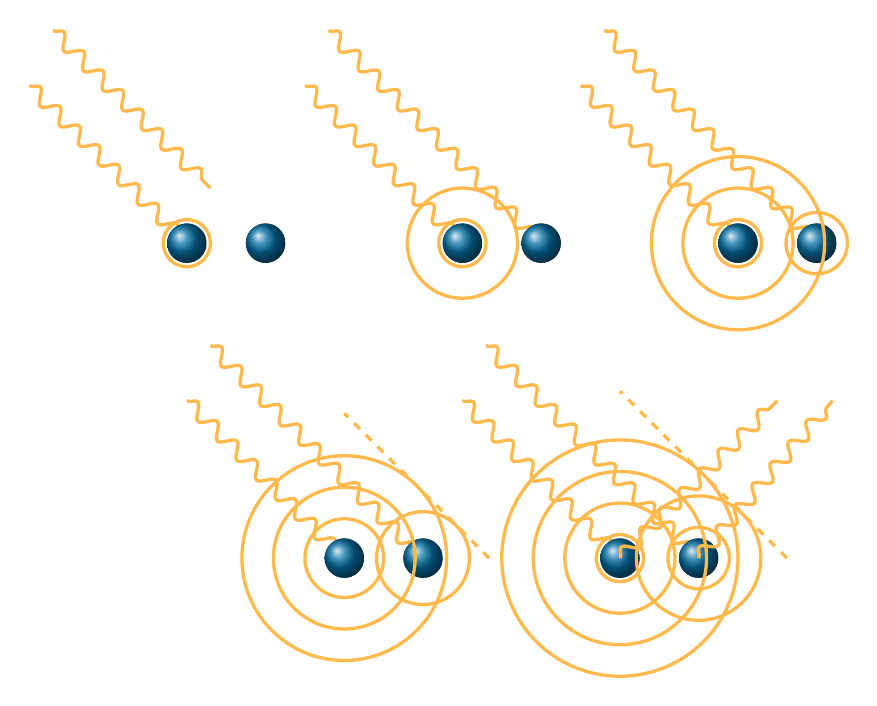
\begin{tikzpicture}
            \tikzset{atom/.style = {ball color=highlight, very thick}}
            \tikzset{wave/.style={complementary, very thick, decoration=snake, decorate}}
            \tikzset{circ/.style={complementary, very thick}}
            \draw[wave] (-2, 2) -- (0, 0);
            \draw[wave] (-1.7, 2.7) -- (0.3, 0.7);
            \fill[atom] (0, 0) circle [radius = 0.25];
            \fill[atom] (1, 0) circle [radius = 0.25];
            \draw[circ] (0, 0) circle [radius = 0.3];
            \begin{scope}[xshift=3.5cm]
                \draw[wave] (-2, 2) -- (0, 0);
                \draw[wave] (-1.7, 2.7) -- (1, 0);
                \fill[atom] (0, 0) circle [radius = 0.25];
                \fill[atom] (1, 0) circle [radius = 0.25];
                \draw[circ] (0, 0) circle [radius = 0.7];
                \draw[circ] (0, 0) circle [radius = 0.3];
            \end{scope}
            \begin{scope}[xshift=7cm]
                \draw[wave] (-2, 2) -- (0, 0);
                \draw[wave] (-1.7, 2.7) -- (1, 0);
                \fill[atom] (0, 0) circle [radius = 0.25];
                \fill[atom] (1, 0) circle [radius = 0.25];
                \draw[circ] (0, 0) circle [radius = 1.1];
                \draw[circ] (0, 0) circle [radius = 0.7];
                \draw[circ] (0, 0) circle [radius = 0.3];
                \draw[circ] (1, 0) circle [radius = 0.39];
            \end{scope}
            \begin{scope}[xshift=2cm, yshift=-4cm]
                \draw[wave] (-2, 2) -- (0, 0);
                \draw[wave] (-1.7, 2.7) -- (1, 0);
                \fill[atom] (0, 0) circle [radius = 0.25];
                \fill[atom] (1, 0) circle [radius = 0.25];
                \draw[circ] (0, 0) circle [radius = 1.3];
                \draw[circ] (0, 0) circle [radius = 0.9];
                \draw[circ] (0, 0) circle [radius = 0.5];
                \draw[circ] (1, 0) circle [radius = 0.59];
                \draw[dashed, circ] (1.84, 0) -- (0, 1.84);
            \end{scope}
            \begin{scope}[xshift=5.5cm, yshift=-4cm]
                \draw[wave] (-2, 2) -- (0, 0);
                \draw[wave] (-1.7, 2.7) -- (1, 0);
                \fill[atom] (0, 0) circle [radius = 0.25];
                \fill[atom] (1, 0) circle [radius = 0.25];
                \draw[circ] (0, 0) circle [radius = 1.5];
                \draw[circ] (0, 0) circle [radius = 1.1];
                \draw[circ] (0, 0) circle [radius = 0.7];
                \draw[circ] (0, 0) circle [radius = 0.3];
                \draw[circ] (1, 0) circle [radius = 0.79];
                \draw[circ] (1, 0) circle [radius = 0.39];
                \draw[dashed, circ] (2.12, 0) -- (0, 2.12);
                \draw[wave] (0, 0) -- (2, 2);
                \draw[wave] (1, 0) -- (2.7, 2);
            \end{scope}
        \end{tikzpicture}
        \caption[Diffraction mechanism]{Two atoms in a crystal absorb and re-emit light.}
    \end{figure}

    \subsection{Bragg's Law}
    \defineindex{Bragg's law} states that for interplanar spacing \(d_{hk\ell}\) and radiation wavelength \(\lambda\) there will be constructive interference at angle \(2\vartheta\) if
    \begin{equation}
        2d_{hk\ell} \sin\vartheta = \lambda
    \end{equation}
    This is the crystallographer's version of Bragg's law, normally there is a factor of \(n \in \integers\) but this isn't needed when we consider whole families of planes at a time.
    
    Bragg's derivation of this law assumes that the crystal planes act like perfect mirrors.
    Further, this law gives us no information about the diffracted intensities and cannot account for systematic absences.
    
    Bragg's law does allow us to determine the unit cell dimensions and hence the lattice part of the crystal structure.
    What it can't do is tell us anything about the arrangement of atoms in this lattice, i.e. the crystal basis.
    For this we will need a fuller description of the diffraction process.
    
    \subsection{The Maths of Diffraction}
    Suppose the incident light is an electromagnetic plane wave with wave vector \(\vv{k}\), that is proportional to \(\e^{i\vv{k}\cdot\vv{r}}\).
    Similarly the diffracted beam is an electromagnetic plane wave with wave vector \(\vv{k'}\), and hence proportional to \(\e^{i\vv{k'}\cdot\vv{r}}\).
    
    We now that \(\abs{\vv{k}} = 2\pi/\lambda\), where \(\lambda\) is the wavelength of the radiation.
    The phase of the wave at \(\vv{r}\) is given by \(\vv{k}\cdot\vv{r}\).
    In a diffraction process there is no change in wavelength and so \(\abs{\vv{k}} = \abs{\vv{k'}} = k\).
    This assumes elastic scattering, meaning the total energy is constant, and since \(E = \hbar c k\) this means \(k\) is constant.
    This is a reasonable assumption as any effects due to inelastic scattering are necessarily weaker due to loss of energy.
    
    Assuming x-ray diffraction the diffraction occurs due to interaction with the electrons.
    We can describe the positions of the electrons with the electron density, \(n(\vv{r})\).
    
    We consider the phase shift at each point in the crystal.
    The phase shift at some point \(\vv{r}\) is \((\vv{k} - \vv{k'})\cdot\vv{r}\).
    We can account for the phase shift from each point of the crystal by integrating over the volume of the crystal.
    This gives us the \defineindex{scattering amplitude}:
    \begin{equation}
        F(\vv{k}, \vv{k'}) = \int\limits_{\text{crystal}} n(\vv{r}) \exp[i (\vv{k} - \vv{k'}) \cdot \vv{r}] \dd{V}.
    \end{equation}
    This measures the strength of diffraction of a wave entering in the direction \(\vh{k}\) and exiting in the direction \(\vh{k}\vv{'}\).
    
    For periodic crystals \(n(\vv{r})\) is periodic in space.
    This suggests that we should use Fourier series.
    
    \subsection{Fourier Series Recap}
    \subsubsection{One Dimension}
    A function is periodic if \(n(x + a) = n(x)\) for all \(x\) for some specific value of \(a\).
    We call \(a\) the period of the function.
    A periodic function can be expanded as a Fourier series.
    In the one-dimensional case the function \(n\) can be expanded as
    \begin{equation}
        n(x) = \frac{1}{2} C_0 + \sum_{p=1}^{\infty} \left[ C_p \cos\left( \frac{1\pi p x}{a} \right) + S_p \sin \left( \frac{2\pi p x}{a} \right) \right].
    \end{equation}
    The coefficients are given by
    \begin{align}
        C_p &= \frac{2}{a} \int_0^a n(x) \cos\left( \frac{2\pi px}{a} \right) \dd{x},\\
        S_p &= \frac{2}{a} \int_0^a n(x) \sin\left( \frac{2\pi px}{a} \right) \dd{x}.
    \end{align}
    
    We can similarly expand \(n\) in a complex Fourier series:
    \begin{equation}
        n(x) = \sum_{p=-\infty}^{\infty} n_p \e^{2\pi i px/a}
    \end{equation}
    where
    \begin{equation}
        n_p = \frac{1}{a}\int_0^a n(x) \e^{-2\pi i px/a}\dd{x}.
    \end{equation}
    If \(n\) is a real function then \(n_{-p} = n_p^*\).
    
    Notice that if \(x\) is a length then \(p\) has units of inverse length.
    
    \subsubsection{Higher Dimensions}
    In two or more dimensions we can do something similar.
    Consider a two-dimensional function \(n\) which is periodic in both of its inputs.
    Then the Fourier series of this function follows very easily from the one dimensional case:
    \begin{equation}
        n(x, y) = \sum_{p, q = -\infty}^{\infty} n_{p,q}\e^{2\pi i px/a}\e^{2\pi i qy/b}
    \end{equation}
    where \(a\) is the period along the \(x\)-axis and \(b\) is the period along the \(y\)-axis.
    An example may be a primitive rectangular lattice with lattice parameters \(a\) and \(b\) where \(n\) is the electron density treating the atoms as points.
    We can define a \defineindex{reciprocal lattice} made of the points
    \begin{equation}
        (2\pi \frac{px}{a}, 2\pi\frac{qy}{b})
    \end{equation}
    for \(p, q \in \integers\).
    
    For a crystal that isn't periodic in the same way we cannot use a Fourier series quite so easily.
    Instead we define a lattice in reciprocal space.
    We define
    \begin{align}
        \vv{a_1^*} &= 2\pi \frac{\vv{a_2}\times\vv{a_3}}{\vv{a_1}\cdot(\vv{a_2}\times\vv{a_3})} = \frac{2\pi}{V} \vv{a_2}\times\vv{a_3},\\
        \vv{a_2^*} &= 2\pi \frac{\vv{a_3}\times\vv{a_1}}{\vv{a_2}\cdot(\vv{a_3}\times\vv{a_1})} = \frac{2\pi}{V} \vv{a_3}\times\vv{a_2},\\
        \vv{a_3^*} &= 2\pi \frac{\vv{a_1}\times\vv{a_2}}{\vv{a_3}\cdot(\vv{a_1}\times\vv{a_2})} = \frac{2\pi}{V} \vv{a_1}\times\vv{a_2}.
    \end{align}
    These are called the \defineindex{reciprocal lattice vectors}.
    We then form a lattice from the points
    \begin{equation}
        \vv{G} = v_1\vv{a_1^*} + v_2\vv{a_2^*} + v_3\vv{a_3^*}
    \end{equation}
    with \(v_i \in \integers\).
    
    Notice that from this definition
    \begin{equation}
        \vv{a_i^*} \cdot \vv{a_j} = 2\pi \delta_{ij}.
    \end{equation}
    
    We call the space described by \(\vv{a_i}\) \enquote{real space}, \enquote{crystal space}, or \enquote{direct space}, and the space described by \(\vv{a_i^*}\) \enquote{reciprocal space}.
    
    Reciprocal lattice vectors have units of inverse length.
    
    \begin{ntn}{Lattice Vector Conventions}{}
        There are a few common conventions for what lattice vectors, and reciprocal lattice vectors, are called:
        \begin{tabular}{ll}\toprule
            \multicolumn{2}{c}{This course}\\
            Real space: & \(\vv{a_1}\), \(\vv{a_2}\), \(\vv{a_3}\)\\
            Reciprocal space: & \(\vv{a_1^*}\), \(\vv{a_2^*}\), \(\vv{a_3^*}\)\\\midrule
            \multicolumn{2}{c}{Kittel (textbook)}\\
            Real space: & \(\vv{a_1}\), \(\vv{a_2}\), \(\vv{a_3}\)\\
            Reciprocal space: & \(\vv{b_1}\), \(\vv{b_2}\), \(\vv{b_3}\)\\\midrule
            \multicolumn{2}{c}{Crystallographer}\\
            Real space: & \(\vv{a}\), \(\vv{b}\), \(\vv{c}\)\\
            Reciprocal space: & \(\vv{a^*}\), \(\vv{b^*}\), \(\vv{c^*}\)\\\bottomrule
        \end{tabular}
    \end{ntn}

    Every crystal therefore has two attached lattices.
    First, the real-space lattice, in which translation vectors, \(\vv{a_i}\), have dimensions of length.
    This lattice tells us abut the periodicity of the atomic arrangement.
    Second, the reciprocal lattice, in which translation vectors, \(\vv{a_i^*}\), have dimensions of inverse length.
    This lattice is a lattice in Fourier space and is useful for dealing with periodic functions, such as charge density, and scattering processes.
    
    All non-centred lattices have the same form in reciprocal space, for example a cubic lattice will have a cubic reciprocal lattice.
    Centred lattices aren't so simple.
    
    We can use the reciprocal lattice to define a Fourier series expansion for \(n(\vv{r})\):
    \begin{equation}
        n(\vv{r}) = \sum_{\vv{G}} = n_{\vv{G}} \e^{i\vv{G}\cdot\vv{r}}
    \end{equation}
    where \(\vv{G} = v_1\vv{a_1^*} + v_2\vv{a_2^*} + v_3\vv{a_3^*}\) with \(v_i\in\integers\).
    The Fourier coefficients are given by
    \begin{equation}
        n_{\vv{G}} = \frac{1}{V_{\text{cell}}} \int_{\mathrlap{\text{unit cell}}} \,n(\vv{r}) \e^{-i\vv{G}\cdot\vv{r}}\dd{V}.
    \end{equation}
    Where \(V_\mathrm{cell}\) is the volume of the unit cell.
    
    \section{The Lattice Vector}
    The reciprocal lattice vector
    \begin{equation}
        \vv{G^*} = h\vv{a_1^*} + k\vv{a_2^*} + \ell\vv{a_3^*}
    \end{equation}
    is perpendicular to the \(\crystalplane{h}{k}{\ell}\) plane.
    To see that this is true we use the fact that this plane intercepts the axes at \(\vv{a_1}/h\), \(\vv{a_2}/k\), and \(\vv{a_3}/\ell\).
    This gives us two vectors \(\vv{a_1}/h - \vv{a_2}/k\) and \(\vv{a_1}/h - \vv{a_3}/\ell\) which are in the plane.
    We can then dot these with \(\vv{G^*}\) and we see we get zero both times.
    This result holds for \emph{all} types of crystals.
    The earlier result that \(h\vv{a_1} + k\vv{a_2} + \ell\vv{a_3}\) is perpendicular to the plane only holds for orthorhombic crystals where all angles are right angles.
    
    The interplanar spacing, \(d_{hk\ell}\), is given by
    \begin{equation}
        d_{hk\ell} = \frac{2\pi}{\abs{\vv{G^*}}}.
    \end{equation}
    To show this is true we we notice that consecutive planes cross the \(\vv{a_1}\) axis at \(\vv{a_1}/h\) and \(2\vv{a_1}/h\) and we use the formula \(\vh{n}\cdot\vv{r} = d\), which gives the distance, \(d\), from the origin for a plane with unit normal \(\vh{n}\) containing the point \(\vv{r}\).
    In our case we use \(\vv{r}\) as the points \(\vv{a_1}/h\), and \(2\vv{a_1}/h\) and \(\vh{n} = \vv{G^*}/\abs{\vv{G^*}}\).
    We then work out the two values of \(d\) and the difference of these is the interplanar spacing.
    This works for \emph{all} types of crystals.
    
    For the special case of orthorhombic crystals (all angles right angles) we can simplify this relationship to get
    \begin{equation}
        \frac{1}{d_{hk\ell}} = \sqrt{\frac{h^2}{a^2} + \frac{k^2}{b^2} + \frac{\ell^2}{c^2}}.
    \end{equation}
    For a cubic crystal (also all sides equal) this simplifies further to
    \begin{equation}
        \frac{1}{d_{hk\ell}} = \sqrt{\frac{h^2 + k^2 + \ell^2}{a^2}}.
    \end{equation}
    
    \section{Diffraction Intensities}
    We shall focus on x-ray diffraction as the most common case but similar work should apply to other types of diffraction.
    In x-ray diffraction electrons absorb x-rays and oscillate.
    They then emit x-rays in all directions (although not with equal intensity).
    We assume that the electron density distribution, \(n(\vv{r})\), is known for a given crystal.
    We then integrate over all contributions to the emitted radiation, accounting for phase differences.
    We will find that most cases cancel out leaving us with only a few diffraction angles at which we get bright spots.
    
    We said previously that the scattering amplitude is
    \begin{equation}
        F(\vv{k}, \vv{k'}) = \int\limits_{\text{crystal}} n(\vv{r})\exp[i(\vv{k} - \vv{k'})\cdot\vv{r}]\dd{V}.
    \end{equation}
    Introducing the \defineindex{scattering vector} \(\vv{\Delta k}\), sometimes denoted \(\vv{Q}\) instead, this becomes
    \begin{equation}
        F_{\vv{\Delta k}} = \int\limits_{\text{crystal}} n(\vv{r}) \e^{-i\vv{\Delta k}\cdot\vv{r}}\dd{V}.
    \end{equation}
    We can recognise this as simply the Fourier transform of the electron density, \(n(\vv{r})\).
    
    Inserting the Fourier expansion of \(n(\vv{r})\) we have
    \begin{align}
        F_{\vv{\Delta k}} &= \int\limits_{\text{crystal}} \sum_{\vv{G}} n_{\vv{G}} \e^{-(\vv{G} - \vv{\Delta k})\cdot\vv{r}}\dd{V}\\
        \sum_{\vv{G}} n_{\vv{G}} \int\limits_{\text{crystal}} \e^{-[\vv{G} - \vv{\Delta k}]\cdot\vv{r}}
    \end{align}
    where we have assumed that the Fourier series converges uniformly and so swapping the sum and integral is valid\footnote{all reasonable physical functions, including the electron density, are smooth enough for uniform convergence of their Fourier series}.
    
    Suppose that \(\vv{G} = \vv{\Delta k}\) for some specific \(\vv{G}\).
    Then for this term in the series we have
    \begin{equation}
        n_{\vv{G}} \int\limits_{\text{crystal}} \dd{V} = n_{\vv{G}}V
    \end{equation}
    where \(V\) is the volume of the crystal.
    
    Now suppose \(\vv{G} \ne \vv{\Delta k}\).
    We then have that \(\abs{\vv{G} - \vv{\Delta k}} \approx 2\pi/\qty{1}{\angstrom} \approx \qty{e11}{m^{-1}}\) and for a typical crystal size of a few millimetres we have \(\abs{\vv{r}} \approx \qty{1}{\milli\meter} \approx \qty{e-3}{\meter}\).
    Hence we find that \(\abs{(\vv{G} - \vv{\Delta k})\cdot\vv{r}} \approx \num{e8}\).
    This is huge.
    The complex exponential factor is then rapidly oscillating.
    The result is that over the entire integral these oscillations cancel out and we get zero.
    
    Combing these two results we have
    \begin{equation}
        F_{\vv{\Delta k}} = 
        \begin{cases}
            n_{\vv{G}}V, &\text{if }\vv{\Delta k} = \vv{G}\text{ for some specific }\vv{G},\\
            0, &\text{else}.
        \end{cases}
    \end{equation}
    As a result we only consider the case when \(\vv{\Delta k} = \vv{G}\) for some \(\vv{G} = h\vv{a_1^*} + k\vv{a_2^*} + \ell\vv{a_3^*}\), which means we only consider \(F_{\vv{G}}\), or in alternative notation \(F_{hk\ell}\).
    This gives rise to the \defineindex{Laue diffraction condition} that \(F_{\vv{\Delta k}} \ne 0\) only if \(\vv{\Delta k} = \vv{G}\).
    
    The diffraction intensity from the plane \(\crystalplane{h}{k}{\ell}\) is \(I_{hk\ell}\) and this is proportional to \(\abs{F_{hk\ell}}^2 = \abs{F_{\vv{G}}}^2 \propto \abs{n_{\vv{G}}}\).
    
    There is an equivalent ways to state the Laue diffraction condition.
    First, rearranging the condition that \(\vv{G} = \vv{\Delta k} = \vv{k'} - \vv{k}\) we have \(\vv{k'} = \vv{k} + \vv{G}\) and so
    \begin{equation}
        \vv{k'}\cdot\vv{k'} = (\vv{k} + \vv{G})\cdot(\vv{k} + \vv{G}) \implies \abs{\vv{k'}}^2 = \abs{\vv{k}}^2 + 2\vv{k}\cdot\vv{G} + \abs{\vv{G}}^2.
    \end{equation}
    This gives \(-2\vv{k}\cdot\vv{G} = \abs{\vv{G}}^2\) since \(\abs{\vv{k}} = \abs{\vv{k'}}\) for elastic scattering.
    WE can then consider a reciprocal lattice vector \(\vv{G'} = -\vv{G}\) in which case we have \(2\vv{k}\cdot\vv{G'} = \abs{\vv{G'}}^2 = G^2\) noticing that \(\vv{G}\) and \(\vv{G'}\) are equivalent when we sum over all lattice vectors we can simply call \(\vv{G'}\) \(\vv{G}\) and we have the condition
    \begin{equation}
        \vv{k}\cdot\vv{G} = \frac{1}{2}\abs{\vv{G}}^2.
    \end{equation}

    From this we can define \(\vartheta_{hk\ell}\) as the angle between \(\vv{k}\) and \(\vv{G}\) and we have
    \begin{equation}
        \vv{k}\cdot\vv{G} = kG\sin\vartheta_{hk\ell} = \frac{1}{2}\abs{\vv{G}}^2 = \frac{1}{2}\left( \frac{2\pi}{d_{hk\ell}} \right)^2.
    \end{equation}
    Noticing that \(k = 2\pi/\lambda\) and \(G = 2\pi/d_{hkl}\) this becomes
    \begin{equation}
        2d_{hk\ell}\sin\vartheta_{hk\ell} = \lambda
    \end{equation}
    and so we have derived \defineindex{Bragg's law} without resorting to assumptions of specular reflection.
    
    \section{Form Factors}
    The diffraction intensity, \(I_{hk\ell}\), is proportional to the magnitude squared of the Fourier coefficients of the electron density.
    Therefore we don't have enough information from the diffraction intensity to recover the Fourier coefficients, and hence to recover the electron density.
    
    In the case when we do have diffraction, i.e. \(\vv{\Delta k} = \vv{G}\), we have the scattering amplitude
    \begin{equation}
        F_{\vv{G}} = \int\limits_{\text{crystal}} n(\vv{r})\e^{-i\vv{G}\cdot\vv{r}}\dd{V}.
    \end{equation}
    If our crystal consists of \(N\) unit cells then this is 
    \begin{equation}
        F_{\vv{G}} = N\int\limits_{\mathrlap{\text{unit cell}}} n(\vv{r})\e^{-i\vv{G}\cdot\vv{r}}\dd{V}.
    \end{equation}
    
    We can approximate \(n(\vv{r})\) as a superposition of free-atom electron densities by neglecting the few electrons that take part in the chemical bonding.
    Doing so and summing over the \(s\) atoms in the unit cell we have
    \begin{equation}
        n(\vv{r}) \approx \sum_{j=1}^{s} n_j(\vv{r} - \vv{r_j})
    \end{equation}
    where \(n_j(\vv{\rho})\) is the free-atom electron density of the \(j\)th atom with \(\vv{\rho}\) being the position taking the centre of the atom, \(\vv{r_j}\), to be the origin.
    
    We can define the \defineindex{atomic form factor}, \(f_j(G)\), to be
    \begin{equation}
        f_j(G) \coloneqq \int n_j(\vv{\rho}) \e^{-i\vv{G}\cdot\vv{\rho}}\dd{V}
    \end{equation}
    where we note that the spherical symmetry of atoms means this is a function of \(G\) rather than \(\vv{G}\).
    The Fourier coefficients are then given by
    \begin{equation}
        F_{\vv{G}} = N\sum_{j=1}^{s} f_j(G)\e^{-i\vv{G}\cdot\vv{r_j}}.
    \end{equation}
    
    In practice it isn't possible to know the exact number of unit cells present in a crystal sample, and we don't need to since we are only interested in proportionality.
    We then define the \defineindex{structure factor}
    \begin{equation}
        S_{hk\ell} = S_{\vv{G}} = \sum_{j=1}^{s} f_j(G)\e^{-i\vv{G}\cdot\vv{r_j}} = \sum_{j} f_j \exp[-2\pi i(hx_j + ky_j + \ell z_j)]
    \end{equation}
    where we take \(\vv{r_j} = x_j\vv{a_1} + y_j\vv{a_2} + z_j\vv{a_3}\) and \(\vv{G} = h\vv{a_1^*} + k\vv{a_2^*} + \ell\vv{a_3^*}\) and used \(\vv{a_i^*}\cdot\vv{a_j} = 2\pi\delta_{ij}\).
    
    It is the structure factor with which we work when considering diffraction.
    We know that
    \begin{equation}
        I_{hk\ell} \propto \abs{S_{hk\ell}}^2
    \end{equation}
    and so we lose information about phase.
    This means that we can't work backwards to find the electron density but this is enough to rule out many crystal structures that are completely wrong.
    
    \section{Diffraction Techniques}
    \subsection{Laue Diffraction}
    Laue diffraction was the original technique for x-ray crystallography.
    In this process \enquote{white} (meaning a range of wavelengths) broadband spectrum x-rays are used.
    A single crystal is used as a sample and is placed in the x-ray beam.
    The diffracted x-rays are collected using some sort of sensor all at once.
    
    This method is best suited to simple crystals, in particular it is often used to ascertain the orientation of a crystal before a more sensitive experiment.
    It is difficult to model the exact intensities of diffraction due to the range of wavelengths.
    
    \subsection{Monochromatic Single Crystal Diffraction}
    This is the modern standard for x-ray crystallography.
    A single crystal is placed in a beam of monochromatic (single wavelength) x-rays.
    The diffracted x-rays are collected as the sample is rotated.
    At any one time x-rays are only diffracted to a few points but by rotating the sample a larger picture can be built up.
    The result is a picture which is mostly dark but with a few bright spots.
    From this it is possible to work out which planes caused the diffraction and from the relative intensities we can measure the magnitude of the structure factor.
    
    For less sensitive work x-ray tubes can produce the required x-ray beams.
    More sensitive work requiring higher energy, more focused beams often uses synchrotron radiation.
    
    \subsection{Monochromatic Powdered Crystal Diffraction}
    Often it is not possible to come up with a single crystal large enough for the procedure in the previous section.
    Instead a polycrystalline powder can be used.
    The setup is otherwise identical.
    Since the crystals in the powder are arranged randomly it is not necessary to rotate the sample.
    A single image can be captured.
    The result will be a series of rings as the crystals diffract in random directions but always at the same angle.
    Integrating around the rings gives the relative intensity, it is not enough to consider the intensity at a point on the ring due to the varying size of the rings.
    It should be possible to assign to each ring the plane from which the diffraction occurred.
    
    \subsection{Atomic Form Factor}
    Diffraction experiments, particularly powder diffraction, will show an overall decrease in intensity with increasing diffraction angle.
    Partly this is geometric, at larger angles the rings are larger and so the same intensity would be spread over a larger area.
    However, the effect remains when taking this into account.
    
    A second factor is destructive interference of x-rays scattered from different parts of the same atom.
    The atomic form factor is the Fourier transform of the charge distribution.
    It describes the interference of waves scattered from different parts of the same atom.
    When we consider x-rays the atomic form factor \(f(0)\) gives the number of electrons in the atom, which can be seen from
    \begin{equation}
        f(0) = \int n(\vv{\rho}) \e^{0} \dd{V}.
    \end{equation}
    Here \(\vv{\rho}\) is the distance from the centre of the atom.
    
    If we take the atoms to be point like scatterers, which is almost the case for neutron diffraction, then the atomic form factors reduce to a constant.
    
    The atomic form factor is a function of \(G\), which, combining Bragg's law and \(d = 2\pi/G\) is given by \(G = 4\pi\sin(\vartheta)/\lambda\).
    The values \(f(\sin(\vartheta)/\lambda)\) are tabulated for all elements.
    
    \subsection{Neutron Diffraction}
    The data produced by neutron diffraction is very similar to that produced by x-ray diffraction.
    The main difference being that x-rays are scattered by the extended electron cloud whereas neutrons are scattered by the nucleus, which is essentially a point particle.
    This results in atomic form factors which are independent of the scattering angle.
    We call these form factors the neutron scattering length.
    The result is that neutrons scattering doesn't have the same drop off with diffraction angle.
    
    Neutrons are generally produced in one of two ways.
    The more old fashioned way is from nuclear reactors.
    More modern setups us spallation sources, which is a fancy way of saying we smash protons into targets at high energy to produce neutrons.
    One issue with neutron diffraction is that neutrons are neutral and therefore we can't use magnetic fields to accelerate them and focus beams in the same way we do with other particles.
    
    \section{Systematic Absences}
    After a diffraction experiment if we have successfully assigned planes to all data points we may see that some planes don't appear.
    These are called \define{systematic absences}\index{systematic absence}.
    These are a result of terms cancelling each other out due to symmetry.
    This is best demonstrated with an example.
    
    \subsection{BCC Systematic Absences}
    Consider a BCC crystal.
    The structure factor is
    \begin{equation}
        S_{hk\ell} = S_{\vv{G}} = \sum_j f_j \e^{-2\pi i(hx_j + ky_j + \ell z_j)}.
    \end{equation}
    We consider the conventional cubic lattice, not the primitive lattice.
    The lattice vectors are \(\vv{a_i} = a\ve{i}\).
    The basis has atoms positioned at \(\vv{r_1} = (0, 0, 0)\), and \(\vv{r_2} = (1/2, 1/2, 1/2)\).
    There is only one type of atom in this simple example and so \(f_1 = f_2 = f\).
    Putting this into the formula for the structure factor we have
    \begin{equation}
        S_{hk\ell} = f[\e^{-2\pi i(0)} + \e^{-2\pi i (h + k + \ell)/2}] = f[1 + \e^{i\pi(h + k + \ell)}].
    \end{equation}
    We see that when \(h + k + \ell\) is odd the second exponential gives \(-1\) and therefore the structure factor is zero:
    \begin{equation}
        S_{hk\ell} = 
        \begin{cases}
            2f, & h + k + \ell \text{ even},\\
            0 & h + k + \ell \text{ odd}.
        \end{cases}
    \end{equation}
    So there is a systematic absence when \(h + k + \ell\) is odd.
    
    We can see this as a result of the symmetry of the crystal, hence why we cannot predict this effect from the lower symmetry primitive cell.
    We find a similar result for an FCC lattice:
    \begin{equation}
        S_{hk\ell} = 
        \begin{cases}
            2f, & \text{\(h\), \(k\), \(\ell\) all odd, or all even},\\
            0, & \text{else}.
        \end{cases}
    \end{equation}
    
    As another example in a C-centre lattice\footnote{recall that this is a lattice with a lattice point at the centre of the C face, that is the face spanned by \(\vv{a}\) and \(\vv{b}\).} we have a systematic absence when \(h + k\) is even.
    
    \section{FCC and BCC Reciprocal Lattices}
    Now that we are discussing diffraction from BCC and FCC crystals while we need to consider the reciprocal lattices for BCC and FCC.
    Recall that non-centred lattices are their own reciprocals, albeit with different lattice parameters.
    
    Consider the primitive cell for an FCC crystal.
    The primitive translation vectors are
    \begin{equation}
        \vv{a_1} = \frac{a}{2}(\vh{y} + \vh{z}), \qquad \vv{a_2} = \frac{a}{2}(\vh{z} + \vh{x}), \qqand \vv{a_3} = \frac{a}{2}(\vh{x} + \vh{y}).
    \end{equation}
    The volume of the primitive cell is
    \begin{equation}
        V = \abs{\vv{a_1} \cdot (\vv{a_2} \times \vv{a_3})} = \frac{1}{4}a^3.
    \end{equation}
    The reciprocal translation vectors are then given by
    \begin{equation}
        \vv{a_1^*} = \frac{2\pi}{V}\vv{a_2}\times\vv{a_3} = \frac{2\pi a^2}{4V}(\vh{x} + \vh{z}) \times (\vh{x} + \vh{y}) = \frac{2\pi}{a}(\vh{z} + \vh{y} - \vh{z})
    \end{equation}
    and similarly
    \begin{equation}
        \vv{a_2^*} = \frac{2\pi}{a}(\vh{x} + \vh{z} - \vh{y}), \qqand \vv{a_3^*} = \frac{2\pi}{a}(\vh{y} + \vh{x} - \vh{z}).
    \end{equation}
    These are simply the translation vectors for some BCC lattice in reciprocal space.
    We see that the reciprocal lattice for a FCC lattice is the BCC lattice, and since the reciprocal of the reciprocal is (up to a constant) the original lattice we know also that the reciprocal of a BCC lattice is the FCC lattice.
    
    \section{Diffraction Beyond Simple Systems}
    \subsection{DNA}
    Perhaps the most important example of x-ray diffraction on a complex system was the determination of the double-helix structure of DNA.
    This was discovered in experiments conducted by Rosalind Franklin.
    However, she was not fully recognised for this work at the time since she was a woman.
    She died before the Nobel prize was awarded to Francis Crick, James Watson, and Maurice Wilkins for their contributions to the discovery of the double helix and it is widely believed that had she been alive she would have been included in this prize.
    
    The key use of x-ray crystallography was to rule out a triple-helix structure that had been suggested.
    Like most x-ray crystallography it wasn't possible to confirm the double-helix structure through x-ray crystallography alone, but it could rule out competing hypotheses.
    
    \subsection{Small Angle Scattering}
    Small angle scattering is a technique used to obtain information about structures with characteristic length in the range \qtyrange{1}{100}{\nano\metre}.
    This covers structures from small viruses down to individual molecules.
    As the name suggests diffraction patterns at low angles, in the range \ang{0.1}--\ang{10}.
    Both x-rays and neutrons can be used, in which case the process is called small angle x-ray scattering (SAXS)\glossary[acronym]{SAXS}{small angle x-ray scattering} or small angle neutron scattering (SANS)\glossary[acronym]{SANS}{small angle neutron scattering}, respectively.
    One advantage of SANS is that neutrons interact more with hydrogen than x-rays do and for biological materials we are often interested in the location of hydrogen atoms.
    
    We saw with crystals that the atomic form factor plays an important role.
    This idea generalises to the notion of a form factor which encodes information about the size and shape of the object being studied.
    In small angle scattering it is conventional to work with the quantity \(Q = 4\pi\sin(\vartheta)/\lambda\), instead of the diffraction angle, \(2\vartheta\).
    
    \subsection{Aperiodic Crystals}
    So far we have only considered periodic crystals, and we will consider to do so for most of the course.
    We would be remiss, however, not to at least mention aperiodic crystals.
    
    It was initially believed that there are no crystals with five-fold symmetry.
    This is related to the idea that regular pentagons cannot tile the plane.
    However, (with the modern definition of crystals based on an essentially sharp diffraction pattern) there have been crystals discovered with 10-fold rotationally symmetric diffraction patterns, and therefore they also necessarily have five-fold rotational symmetry.
    The first example being a crystal made of zinc, magnesium and holmium.
    The existence of such a crystal is related to the ability to tile the plane aperiodically with five-fold symmetry, the most famous example using Penrose tiles.
    
    \begin{figure}
        \tikzsetnextfilename{penrose-tiling}
        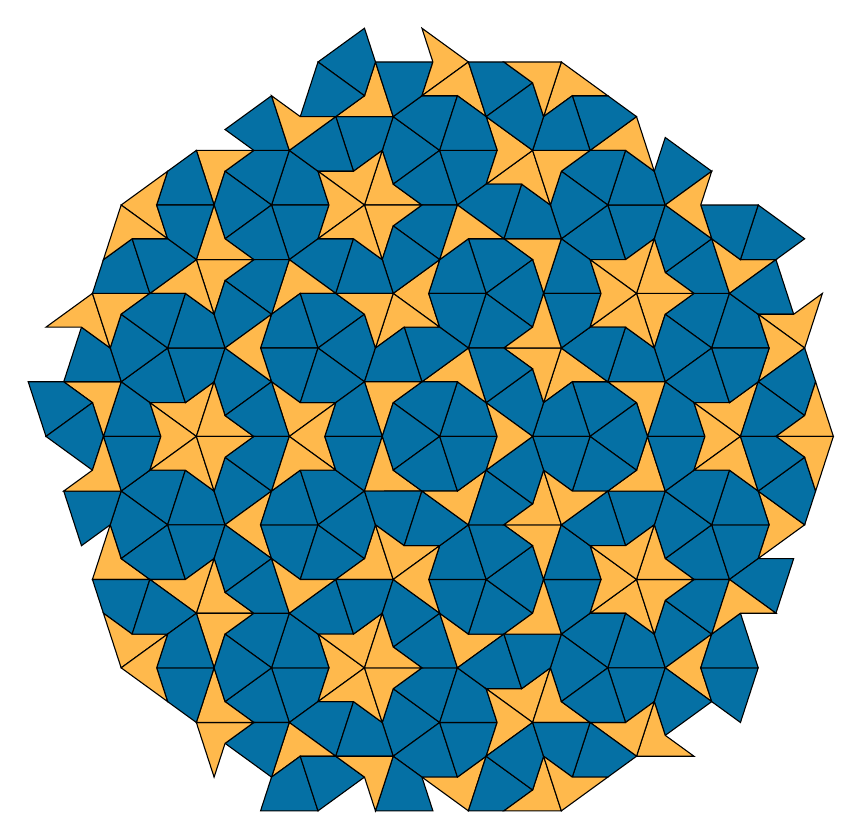
\begin{tikzpicture}[
                every Penrose tile/.style={draw},
                every kite/.style={fill=highlight},
                every dart/.style={fill=complementary}
            ]
            \foreach[evaluate=\k as \mk using {\k+Mod(\k,2)},evaluate=\k as
            \ax using {Mod(\k,2) == 0 ? "T" : "t"}] \k in {0,...,9} {
                \begin{scope}[rotate=\mk*36]
                    \PenroseDecomposition[Penrose step=5cm]{kite}{4}{\ax}
                \end{scope}
            }
        \end{tikzpicture}
        \caption[Aperiodic Penrose tiling.]{An aperiodic tiling of the plane with five-fold symmetry, known as a Penrose tiling.}
    \end{figure}
    
    Aperiodic crystals are often called \defineindex{quasicrystals}, since they don't fit earlier definitions of crystals.
    Since their first discovery many other examples have been found.
    
    \chapter{Crystal Binding}\label{sec:crystal binding}
    So far we've considered the shape of various crystals, but not why they form these shapes.
    To answer this we need to understand what holds crystals together.
    It's then a case of finding a minimum energy structure and over time a crystal will tend towards this form.
    There are four types of bonding that we need to consider.
    These are
    \begin{enumerate}
        \item Van der Waals' forces
        \item Ionic bonding
        \item Covalent bonding
        \item Metallic bonding
    \end{enumerate}
    Real crystals usually have a mixture of these.
    Van der Waals forces are the weakest and appear predominantly in noble gas crystals, since they are vastly overshadowed by any other bonding.
    Ionic bonds form between metals and non-metals when they exchange electrons to form ions which then attract each other.
    Covalent bonds form between non-metals when they share electrons, which they are both attracted to.
    Metallic bonds form, obviously, between metals where they lose electrons to form a sea of electrons and the resulting positive ions are then bound to this sea.
    
    When measuring bond strength force is not a very good measure since the force depends on the distance.
    Instead a better measure is the change in energy between a free system, with no interactions, and the system with interactions.
    A negative change in energy means that the interaction is attractive as the bound state is energetically favourable.
    On the other hand, a positive energy change means that the interaction is repulsive.
    
    Typically binding energies are
    \begin{enumerate}
        \item \(\sim\qty{0.1}{\electronvolt}\) per atom for rare gas crystals,
        \item \(\sim\qty{1}{\electronvolt} \) per atom for alkali metals,
        \item \(\sim\qtyrange{1}{10}{eV/atom}\) for other elemental crystals, and
        \item \(\sim\qtyrange{2}{6}{eV/atom}\) for ionic crystals.
    \end{enumerate}
    These are the \define{cohesive energies}\index{cohesive energy} of the crystals.
    They are defined as the energy required to form separated neutral atoms from the crystal.
    Precisely this requires moving the atoms infinitely far apart but in practice almost all of the energy is needed for just a small separation.
    
    \section{Van der Waals}
    \subsection{Attractive Component}
    The \defineindex{van der Waals} interaction is important in weakly bound crystals, such as noble-gas crystals, and also in soft matter, for example, when considering colloidal suspensions.
    They can even have microscopic effects, such as allowing Gecko's feet to stick to walls.
    Van der Waals interactions are present in all crystals but other interactions are much stronger if they are present.
    
    The mechanism behind the attractive component of the van der Waals interaction is instantaneous dipoles.
    In general we can model atoms as two charges, a positive charge fixed at a nucleus and a negative charge at the centre of the electron cloud.
    This negative charge is not stationary but moves around slightly due to random fluctuations in charge density.
    The charge separation results in an instantaneous dipole.
    If there is a nearby atom then this will induce in the atom a dipole aligned such that the two atoms attract each other.
    
    Of course this atom also has random fluctuations in charge density and so is forming its own instantaneous dipoles and interacting with its neighbours and so on.
    
    \subsubsection{Oscillator Model}
    We are interested in the attractive interaction between two dipoles.
    We can model these as quantum harmonic oscillators, see \cref{fig:dipole oscillators}.
    Each formed from two charges, \(\pm e\), which represent the charge of the nucleus and the valence electron.
    These are connected by a spring, which models the attraction between the charges.
    We fix the positive charges at some length \(R\), which is the nuclear separation.
    Each pair of charges is separated by \(x_i\).
    We want to know how the energy of the system changes as the dipoles are brought closer together.
    We will see that the solution is \(E \propto R^{-6}\).
    
    \begin{figure}
        \tikzsetnextfilename{double-dipole-oscillator}
        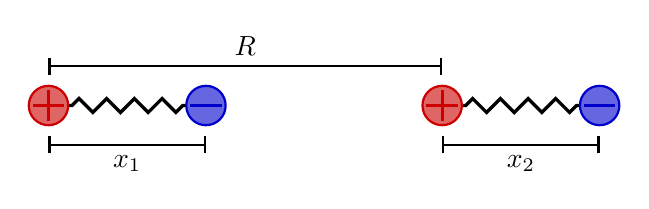
\begin{tikzpicture}
            \tikzset{charge/.style={draw, thick, #1, fill=#1!60, circle, minimum size=0.5cm, inner sep=0pt, font={\large}}}
            \tikzset{spring/.style={decoration={zigzag, pre length=0.3cm, post length=0.2cm}, decorate, very thick}}
            \draw[spring] (0, 0) -- (2, 0);
            \draw[spring] (5, 0) -- (7, 0);
            \node[charge=positive red] {};
            \node[charge=negative blue] at (2, 0) {};
            \node[charge=positive red] at (5, 0) {};
            \node[charge=negative blue] at (7, 0) {};
            \draw[positive red, very thick] (-0.2, 0) -- (0.2, 0);
            \draw[positive red, very thick] (0, -0.2) -- (0, 0.2);
            \draw[positive red, very thick] (4.8, 0) -- (5.2, 0);
            \draw[positive red, very thick] (5, -0.2) -- (5, 0.2);
            \draw[negative blue, very thick] (1.8, 0) -- (2.2, 0);
            \draw[negative blue, very thick] (6.8, 0) -- (7.2, 0);
            
            \draw[|-|, thick] (0, 0.5) -- (5, 0.5) node[midway, above] {\(R\)};
            \draw[|-|, thick] (0, -0.5) -- (2, -0.5) node[midway, below] {\(x_1\)};
            \draw[|-|, thick] (5, -0.5) -- (7, -0.5) node[midway, below] {\(x_2\)};
        \end{tikzpicture}
        \caption[Dipole oscillators and van der Waals interactions.]{The two dipole oscillators used to model van der Waals interactions.}
        \label{fig:dipole oscillators}
    \end{figure}
    
    We start by considering the unperturbed system.
    This is equivalent to considering the case of \(R = \infty\).
    The Hamiltonian for the unperturbed system is
    \begin{equation}
        \hamiltonian_0 = \frac{p_1^2}{2m} + \frac{1}{2}Cx_1^2 + \frac{p_2^2}{2m} + \frac{1}{2}Cx_2^2.
    \end{equation}
    This is simply the sum of the two independent oscillator's Hamiltonians.
    The natural frequency of these oscillators, \(\omega_0\), relates to the constant \(C\) by \(C = m\omega_0^2\).
    The energy of a single oscillator in the \(n\)th excited state is
    \begin{equation}
        E_n = \left( n + \frac{1}{2} \right) \hbar\omega_0
    \end{equation}
    with\footnote{\(\naturals \coloneqq \{0, 1, 2, \dotsc\}\)} \(n \in \naturals\).
    It follows that the zero-point energy (ZPE)\glossary[acronym]{ZPE}{zero-point energy} of the two oscillator system is
    \begin{equation}
        E_0 = 2 \cdot\frac{1}{2}\hbar\omega_0.
    \end{equation}
    
    We can now add in a perturbation to the Hamiltonian corresponding to the interactions between the charges.
    The perturbation Hamiltonian is simply the sum of the Coulomb interactions between the pairs of charged particles:
    \begin{equation}
        \hamiltonian_1 = \frac{e^2}{R} + \frac{e^2}{R + x_1 - x_2} - \frac{e^2}{R + x_1} - \frac{e^2}{R - x_2}. \CGS
    \end{equation}

    \begin{rmk}
        This equation is in \defineindex{CGS} units, we will flag equations in CGS units with \CGSpic{} throughout.
        The CGS system of units uses centimetres, grams and seconds\glossary[acronym]{CGS}{centimetre, gram, second} as base units, as opposed to the SI\glossary[acronym]{SI}{syst\`eme international}, which uses metres, kilograms, and seconds.
        To convert this equation from CGS to SI replace \(e^2\) with \(e^2/(4\pi\varepsilon_0)\).
    \end{rmk}
    
    Returning to the problem at hand, this Hamiltonian is not easy to deal with.
    Assuming that \(\abs{x_1}, \abs{x_2} \ll R\) we can combine the terms over a common denominator and drop all but the highest order term.
    This leaves us with
    \begin{equation}
        \hamiltonian_1 \approx -\frac{2e^2x_1x_2}{R^3}.
    \end{equation}
    
    We can now consider the Hamiltonian for the full system:
    \begin{equation}
        \hamiltonian = \hamiltonian_0 + \hamiltonian_1 = \frac{p_1^2}{2m} + \frac{1}{2}Cx_1^2 + \frac{p_2^2}{2m} + \frac{1}{2}Cx_2^2 - \frac{2e^2x_1x_2}{R^3}.\CGS
    \end{equation}
    This is easiest to work with if we diagonalise.
    To do this we introduce a normal mode transformation defining
    \begin{equation}
        x_{\mathrm{s}} \coloneqq \frac{1}{\sqrt{2}}(x_1 + x_2), \qqand x_{\mathrm{a}} \coloneqq \frac{1}{\sqrt{2}}(x_1 - x_2).
    \end{equation}
    Similarly we define the momenta
    \begin{equation}
        p_{\mathrm{s}} \coloneqq \frac{1}{\sqrt{2}}(p_1 + p_2), \qqand p_{\mathrm{a}} \coloneqq \frac{1}{\sqrt{2}}(p_1 - p_2).
    \end{equation}
    We can rearrange these to find \(x_i\) and \(p_i\):
    \begin{align}
        x_1 &= \frac{1}{\sqrt{2}}(x_{\mathrm{s}} + x_{\mathrm{a}}), \qquad & x_2 &= \frac{1}{\sqrt{2}}(x_{\mathrm{s}} - x_{\mathrm{a}}),\\
        p_1 &= \frac{1}{\sqrt{2}}(p_{\mathrm{s}} + p_{\mathrm{a}}), \qquad & p_2 &= \frac{1}{\sqrt{2}}(p_{\mathrm{s}} - p_{\mathrm{a}}).
    \end{align}
    Substituting these into the Hamiltonian and simplifying gives
    \begin{equation}
        \hamiltonian = \frac{p_{\mathrm{s}}^2}{2m} + \frac{1}{2}\underbrace{\left( C - \frac{2e^2}{R^3} \right)}_{\eqqcolon m\omega_{\mathrm{s}}^2}x_{\mathrm{s}}^2 + \frac{p_{\mathrm{a}}^2}{2m} + \frac{1}{2}\underbrace{\left( C + \frac{2e^2}{R^3} \right)}_{\eqqcolon m\omega_{\mathrm{a}}^2}x_{\mathrm{a}}^2. \CGS
    \end{equation}

    We see that this is the sum of two independent oscillators with frequencies
    \begin{equation}
        \omega_{\mathrm{a}, \mathrm{s}} = \sqrt{\frac{1}{m}\left( C \pm \frac{2e^2}{R^3} \right)} = \omega_0 \sqrt{1 \pm \frac{2e^2}{CR^3}}. \CGS
    \end{equation}
    Using the Taylor expansion, \(\sqrt{1 + \varepsilon} \approx 1 + x/2 - x^2/8\), this becomes
    \begin{equation}
        \omega_{\mathrm{a}, \mathrm{s}} \approx \omega_0\left[ 1 \pm \frac{1}{2}\frac{2e^2}{CR^3} - \frac{1}{8}\left( \frac{2e^2}{CR^3} \right)^2 \right]. \CGS
    \end{equation}
    The total zero-point energy of the coupled system is then
    \begin{equation}
        E_0' = \frac{1}{2}\hbar\omega_{\mathrm{s}} + \frac{1}{2}\hbar\omega_{\mathrm{a}} = \hbar\omega_0\left[ 1 - \frac{1}{8}\left( \frac{2e^2}{CR^3} \right)^2 \right] = \hbar\omega_0\left( 1 - \frac{A}{R^6} \right) \CGS
    \end{equation}
    where
    \begin{equation}
        A = \frac{1}{8}\left( \frac{2e^2}{C} \right)^2. \CGS
    \end{equation}
    
    Recall that the zero point energy of the uncoupled system is \(E_0 = \hbar\omega_0\) and we see that the reduction in energy due to the coupling is
    \begin{equation}
        \Delta U = E_0' - E_0 = -\frac{A}{R^6}.
    \end{equation}
    This is negative and hence corresponds to an attractive interaction.
    The binding energy varies as \(R^{-6}\) and the attractive force,
    \begin{equation}
        F = -\diff{\Delta U}{R},
    \end{equation}
    varies as \(R^{-7}\).
    
    This attractive interaction depends on the zero-point energy of the system and hence is an inherently quantum effect.
    
    This interaction is known under a few names.
    We have been calling it the van der Waals interaction, after Johannes van der Waals, the experimentalist who discovered the effect.
    It is also sometimes called the \define{London interaction}\index{London interaction|see{van der Waals}}, after Fritz London, the theorist who first explained it.
    At the time of solving this problem London was working on the dispersion of light in glass and the relation of wave length and index of refraction, this can also be explained by the oscillator model of an atom.
    See the notes from the optics part of the Electromagnetism course.
    For this reason these are also sometimes called the \define{dispersion interaction}\index{dispersion interaction|see{van der Waals}}.
    The mechanism of inducing dipoles means that these are also called \define{induced dipole-dipole interactions}\index{induced dipole-dipole interaction|see{van der Waals}}.
    
    \subsection{Repulsive Term}
    The van der Waals interaction is entirely attractive.
    Yet, atoms don't all collapse to a single point.
    There must be some repulsive force we have not accounted for.
    It would not be unreasonable to assume that this comes from the Coulomb interaction between the positively charged nuclei.
    However, there is a far greater source of repulsion, from the Pauli exclusion principle.
    
    As the two nuclei are brought together their wave functions start to overlap.
    As a result the Pauli exclusion principle applies to \emph{all} electrons in the combined two-atom system.
    Assuming that both atoms start in their ground states the only way to combine the wave functions is to have some electrons become excited so that they aren't in the same state.
    This requires energy, meaning the potential energy increases, and hence the result is a repulsive force.
    
    To see an example of this consider combining two hydrogen atoms with their electrons both in the ground state, 1s, but with opposite spins.
    When combined we get a \ce{^2He} atom with two electrons, both in the ground state 1s and with opposite spins.
    The total electron energy is \qty{-78.98}{\electronvolt}.
    A similar situation with two electrons with aligned spins can only occur if upon merging one of the electrons is excited to 2s (note that the spin can't flip as we must conserve angular momentum).
    The total electron energy is then \qty{-59.38}{\electronvolt}.
    This is an increase in energy of \qty{-19.6}{\electronvolt}.
    For comparison in hydrogen the electron is only bound with \qty{-13.6}{\electronvolt} in its ground state.
    
    We can capture the essential features of this repulsive effect with an empirical potential.
    These are potentials which we use through no justification other than they work.
    One common potential is
    \begin{equation}
        U(R) = \lambda\e^{-R/\rho}
    \end{equation}
    where \(R\) is the internuclear separation, and \(\lambda\) and \(\rho\) are constants of some characteristic energy and length scale.
    A simpler potential which we will make use of is
    \begin{equation}
        U(r) = \frac{B}{R^{12}}
    \end{equation}
    where \(B\) is some constant.
    There is nothing particularly important about the exponent being 12.
    Models with \(R^{-10}\), for example, would work just as well with a different constant.
    The choice of 12 is mostly for computational efficiency, especially in the pre-computer days.
    Once we have calculated \(R^{-6}\) for the attractive component computing \(R^{-12}\) is as simple as squaring this result.
    
    \subsection{Lennard-Jones Potential}
    The \defineindex{Lennard-Jones potential} is the result of combining both the attractive and repulsive interactions.
    It is
    \begin{equation}
        U_{\LJ}(R) = 4\varepsilon\left[ \left( \frac{\sigma}{R} \right)^{12} - \left( \frac{\sigma}{R} \right)^{6} \right]
    \end{equation}
    where \(\varepsilon\) and \(\sigma\) are parameters related to the energy and length scale respectively.
    This describes the interaction between a \emph{single pair} of atoms.
    
    The minimum of the potential, that is the equilibrium interatomic distance for a diatomic Lennard-Jones molecule, is found by differentiation:
    \begin{align}
        0 &= \diff{U_{\LJ}}{R}[R=r_0]\\
        &= 4\varepsilon\left[ -12\frac{\sigma^{12}}{r_0^{13}} + 6\frac{\sigma^{6}}{r_0^{7}} \right]\\
        \implies 12\frac{\sigma^{12}}{r_0^{13}} &= 6\frac{\sigma^{6}}{r_0^{7}}\\
        \implies \frac{\sigma^{6}}{r_0^{6}} &= \frac{1}{2}\\
        \implies \frac{r_0}{\sigma} &= 2^{1/6} \approx 1.12246.
    \end{align}
    
    \section{Van der Waals Crystal}
    We now have the Lennard-Jones potential, describing the interaction between \emph{pairs} of atoms due to van der Waals interactions and the repulsive effect of Pauli's exclusion principle.
    To consider an entire crystal we need to consider all pairwise interactions between atoms.
    Start by numbering all atoms to give them names.
    We take some reference atom, \(i\), and we sum over all atoms, \(j\), apart from \(i\).
    For each term of the sum we calculate the potential, \(U_{\LJ}(r_{ij})\), where \(r_{ij}\) is the distance between atom \(i\) and atom \(j\).
    This calculates all pairwise interactions with atom \(i\).
    If we do this for every atom one at a time taking the role of the reference atom then the result will be \emph{twice} the total potential of the entire crystal.
    The result is two times too large since we have double counted the interaction between \(i\) and \(j\) and the interaction between \(j\) and \(i\).
    For this reason we add in a factor of \(1/2\).
    In maths the process we've just described is
    \begin{equation}
        U_{\tot} = \frac{1}{2}\sum_{i=1}^{N} \sum_{j\ne i} U_{\LJ}(r_{ij}).
    \end{equation}
    
    Assuming that \(N\) is large and the potential drops away with distance only the nearby atoms are important.
    The ordered nature of the crystal means that most atoms are in a similar configuration of nearby atoms.
    The exception is for atoms on or near the surface of the crystal.
    However, the number of surface atoms goes with the square of the crystal size and the number of interior atoms goes with the cube.
    Therefore for all but the smallest crystals we can treat the surface atoms as interior atoms and the error will be relatively small.
    The result is that each term of the sum over \(i\) is approximately the same and so we make the approximation
    \begin{equation}
        U_{\tot} = \frac{N}{2}\sum_{j\ne i} U_{\LJ}(r_{ij})
    \end{equation}
    where we now choose some random interior atom to be \(i\).
    
    Substituting in the full potential we have
    \begin{equation}
        U_{\tot} = \frac{N}{2}4\varepsilon \left[ \sum_{j\ne i}\left( \frac{\sigma}{r_{ij}} \right)^{12} - \sum_{j\ne i} \left( \frac{\sigma}{r_{ij}} \right)^{6} \right].
    \end{equation}
    We want to come up with a formula that we can apply to any lattice.
    For this reason we define \(r_{ij} = Rp_{ij}\) where \(R\) is the minimum interatomic spacing in the crystal, that is the nearest neighbour distance.
    This allows us to factor out the crystal-specific information from the sums leaving us with
    \begin{equation}
        U_{\tot}(R) = \frac{N}{2}4\varepsilon\bigg[ \left( \frac{\sigma}{R} \right)^{12} \underbrace{\sum_{j\ne i} \frac{1}{p_{ij}^{12}}}_{\eqqcolon a_{12}} - \left( \frac{\sigma}{R} \right)^6 \underbrace{\sum_{j\ne i} \frac{1}{p_{ij}^6}}_{\eqqcolon a_6} \bigg].
    \end{equation}
    Here we have defined the \defineindex{lattice sums}, \(a_6\) and \(a_{12}\):
    \begin{equation}
        a_{n} \coloneqq \sum_{j\ne i} \frac{1}{p_{ij}^n}.
    \end{equation}
    
    \subsection{Lattice Sums}
    \subsubsection{Two Dimensions}
    We will start with an example of a lattice sum in two dimensions, as these are easier to visualise.
    For geometrical simplicity we consider a square crystal.
    \Cref{fig:2d lattice sum} shows a reference atom and the distances to its five nearest neighbours.
    We can also count the number of nearest neighbours from this diagram.
    Since each nearest neighbour of a given order is the same distance from the reference atom we can combine the terms of the sum corresponding to the nearest neighbours.
    Going up to the fifth nearest neighbours we get have
    \begin{align}
        a_{12} &= \frac{4}{1^{12}} + \frac{4}{\sqrt{2}^{12}} + \frac{4}{2^{12}} + \frac{8}{\sqrt{5}^{12}} + \frac{4}{\sqrt{8}^{12}} + \dotsb\\
        &\approx 4 + 0.0625 + 0.000977 + 0.000512 + \dotsb\\
        &\approx 4.064.
    \end{align}
    
    \begin{figure}
        \tikzsetnextfilename{2d-lattice-sum}
        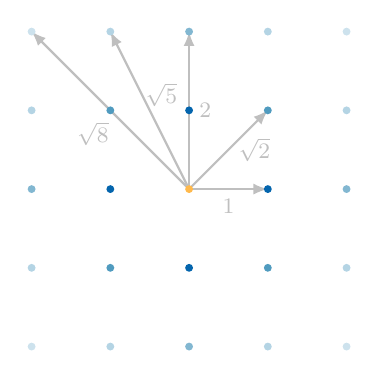
\begin{tikzpicture}
            \tikzset{lattice point/.style={inner sep=0pt, minimum size=0.1cm, circle}};
            \tikzset{arrow/.style={->, lightgray, thick, font={\footnotesize}}}
            \draw[arrow] (0, 0) -- (1, 0) node[midway, below] {\(1\)};
            \draw[arrow] (0, 0) -- (1, 1) node[midway, right] {\(\sqrt{2}\)};
            \draw[arrow] (0, 0) -- (0, 2) node[midway, right] {\(2\)};
            \draw[arrow] (0, 0) -- (-1, 2);
            \draw[arrow] (0, 0) -- (-2, 2);
            \node[lightgray, font={\footnotesize}] at (-0.35, 1.2) {\(\sqrt{5}\)};
            \node[lightgray, font={\footnotesize}] at (150:1.41) {\(\sqrt{8}\)};
            % Reference atom
            \node[lattice point, fill=complementary] at (0, 0) {};
            % 1st NN
            \node[lattice point, fill=highlight!90!blue] at (0, 1) {};
            \node[lattice point, fill=highlight!90!blue] at (0, -1) {};
            \node[lattice point, fill=highlight!90!blue] at (1, 0) {};
            \node[lattice point, fill=highlight!90!blue] at (-1, 0) {};
            % 2nd NN
            \node[lattice point, fill=highlight!70] at (1, 1) {};
            \node[lattice point, fill=highlight!70] at (1, -1) {};
            \node[lattice point, fill=highlight!70] at (-1, 1) {};
            \node[lattice point, fill=highlight!70] at (-1, -1) {};
            % 3rd NN
            \node[lattice point, fill=highlight!50] at (0, 2) {};
            \node[lattice point, fill=highlight!50] at (0, -2) {};
            \node[lattice point, fill=highlight!50] at (2, 0) {};
            \node[lattice point, fill=highlight!50] at (-2, 0) {};
            % 4th NN
            \node[lattice point, fill=highlight!30] at (2, 1) {};
            \node[lattice point, fill=highlight!30] at (2, -1) {};
            \node[lattice point, fill=highlight!30] at (-2, 1) {};
            \node[lattice point, fill=highlight!30] at (-2, -1) {};
            \node[lattice point, fill=highlight!30] at (1, 2) {};
            \node[lattice point, fill=highlight!30] at (1, -2) {};
            \node[lattice point, fill=highlight!30] at (-1, 2) {};
            \node[lattice point, fill=highlight!30] at (-1, -2) {};
            % 5th NN
            \node[lattice point, fill=highlight!20] at (2, 2) {};
            \node[lattice point, fill=highlight!20] at (2, -2) {};
            \node[lattice point, fill=highlight!20] at (-2, 2) {};
            \node[lattice point, fill=highlight!20] at (-2, -2) {};        \end{tikzpicture}
        \caption[Lattice distances for lattice sums.]{A square crystal with distances from some reference atom.}
        \label{fig:2d lattice sum}
    \end{figure}
    
    From this we can see that the lattice sum is approximately the number of nearest neighbours with a small correction for the second nearest neighbours and an even smaller correction for the third nearest neighbours and so on.
    
    \subsubsection{Three Dimensions}
    A similar process can be applied to three-dimensional crystal structures, although the geometry is slightly more complicated.
    Again, we would find that each lattice sum is essentially the number of nearest neighbours with small corrections, although the corrections are slightly large than the two-dimensional case since the number of nearest neighbours goes with distance squared in the three-dimensional case but only with distance in the two-dimensional case.
    
    Fortunately people have already calculated the lattice sums for common lattices to far more precision than we could reasonably do.
    They found
    \begin{align}
        &\text{FCC:} \qquad & a_{12} &= 12.13188, \quad & a_{6} = 14.45392,\\
        &\text{HCP:} \qquad & a_{12} &= 12.13229, \quad & a_{6} = 14.45489,\\
        &\text{BCC:} \qquad & a_{12} &= 9.11418, \quad & a_{6} = 12.2533.
    \end{align}
    Notice that FCC and HCP have almost identical lattice sums.
    This is because the dominant effect in the lattice terms is the distance to nearest neighbours, which in turn is linked to the packing density, and the packing density of FCC and HCP is the same.
    It should also be noted that \(a_{12}\) is approximately the number of nearest neighbours, also known as the \defineindex{coordination number}.
    Both FCC and HCP have a coordination number of 12.
    BCC has a coordination number of 8.
    The discrepancy between \(a_{12} \approx 9.1\) and the coordination number 8 is due to the fact that the second nearest neighbours in a BCC crystal aren't that much further away than the nearest neighbours and therefore have a non-negligible contribution to the lattice sum.
    
    \subsection{Van der Waals Crystal Properties}
    Returning now to the potential we can find the equilibrium interatomic spacing in a crystal by finding the minimum of the potential:
    \begin{align}
        0 &= \diff{U_{\tot}}{R}[R=R_0]\\
        &= 2N\varepsilon\left[ -12a_{12}\frac{\sigma^{12}}{R_0^{13}} + 6a_6\frac{\sigma^{6}}{R_0^{7}} \right]\\
        \implies 12a_{12}\frac{\sigma^{12}}{R_0^{13}} &= 6a_6\frac{\sigma^{6}}{R_0^{7}}\\
        \implies \frac{\sigma^6}{R_0^6} &= \frac{a_{6}}{2a_{12}}\\
        \implies \frac{\sigma}{R_0} &= \left( \frac{a_6}{2a_{12}} \right)^{1/6}.
    \end{align}
    For comparison the interatomic spacing between two otherwise free atoms gave us \(r_0/\sigma = 2^{1/6} \approx 1.12\).
    For FCC and HCP we find that \(R_0/\sigma \approx 1.09\) and for BCC \(R_0/\sigma \approx 1.07\).
    We see that the interatomic spacing decreases slightly from the free diatomic molecule.
    
    In general the potential energy at equilibrium is
    \begin{equation}
        U_{\tot}(R_0) = 2N\varepsilon\left[ \left( \frac{a_6}{2a_{12}} \right)^{12} \right]a_{12} - \left( \frac{a_6}{2a_{12}} \right) = -4\varepsilon N\frac{a_6^2}{4a_{12}}.
    \end{equation}
    A more useful quantity is the binding energy per atom
    \begin{equation}
        U_0 = \frac{1}{N}U_{\tot}(R_0) = -4\varepsilon N\frac{a_6^2}{8a_{12}}.
    \end{equation}
    Evaluating this for FCC, HCP, and BCC crystals we find
    \begin{equation}
        \text{FCC:} \ -2.1525\cdot 4\varepsilon, \quad \text{HCP:} \ -2.1582\cdot 4\varepsilon, \qand \text{BCC:} \ -2.0592\cdot 4\varepsilon.
    \end{equation}
    From this we see that FCC and HCP are the most stable van der Waals crystals.
    The small difference between their binding energies per atom is negligible compared to approximations made in the derivation.
    
    This observation is born out in reality.
    When we cool the noble gases, \ce{Ne}, \ce{Ar}, \ce{Kr}, and \ce{Xe} down to a few kelvin they do indeed form FCC crystals.
    The lightest noble gas, \ce{He}, doesn't form a solid, even at absolute zero.
    This is because its zero-point energy is higher than the very small binding energy provided by van der Waals interactions.
    If we increase the pressure, essentially artificially decreasing interatomic spacing and hence increasing the strength of van der Waals interactions, then \ce{He} does form a crystal structure and this too agrees with our prediction that FCC and HCP are preferentially selected for by energy minimisation.
    
    \section{Ionic Binding}
    \subsection{Cohesive Energy}
    Recall that when we defined cohesive energy at the start of the chapter (\cref{sec:crystal binding}) we defined it as the energy required to separate a crystal into its \emph{neutral} constituent atoms.
    For an ionic crystal this means we need to consider not only the binding energy but also the energy required to create the ions from the neutral atoms.
    That is the ionisation energy for the positive ions and electron affinity for the negative ions.
    
    Consider, for example, \ce{NaCl}.
    This is formed from \ce{Na^+} ions and \ce{Cl^-} ions.
    We make the \ce{Na^+} ions in the reaction
    \begin{equation}
        \ce{Na_{\mathrm{g}}} + \text{Ionisation energy: \qty{5.14}{\electronvolt}} \longrightarrow \ce{Na^+_{\mathrm{g}}} + \Pe.
    \end{equation}
    Here the subscript \(\mathrm{g}\) denotes that we consider a gas of sodium atoms and ions, this is simply because this allows us to treat the interactions between atoms/ions as negligible.
    We make the \ce{Cl^-} ions in the reaction
    \begin{equation}
        \ce{Cl_{\mathrm{g}}} + \Pe \longrightarrow \ce{Cl^-_{\mathrm{g}}} + \text{Electron affinity: \qty{3.61}{\electronvolt}}.
    \end{equation}
    Note that both energies above are per atom/ion.
    We then form a single \ce{NaCl} unit in the reaction
    \begin{equation}
        \ce{Na^+_{\mathrm{g}}} + \ce{Cl^-_{\mathrm{g}}} \longrightarrow \ce{NaCl_{\mathrm{crystal}}} + \text{Binding energy: \qty{7.9}{\electronvolt}}.
    \end{equation}
    Combining these we see that when creating \ce{NaCl} from gaseous sodium and chlorine the energy change is
    \begin{equation}
        \qty{5.1}{\electronvolt} - \qty{3.6}{\electronvolt} - \qty{7.9}{\electronvolt} = -\qty{6.4}{\electronvolt}
    \end{equation}
    per \ce{NaCl} unit.
    Hence the cohesive energy of \ce{NaCl} is \qty{6.4}{\electronvolt} per \ce{NaCl} unit.
    We call this the energy per formula unit, sometimes abbreviated as \unit{\eVperFormulaUnit}.
    
    In reality in standard conditions chlorine forms a gas but sodium is in a metallic state.
    However, the cohesive energy of sodium metal is only \qty{1.1}{\eVperAtom}, and so creating \ce{NaCl} from the elements in their normal forms is still energetically favourable.
    
    One of the reasons that the ionic \ce{NaCl} is more stable than the elemental forms is that in the process of forming the ions both \ce{Na} and \ce{Cl} achieve full outer shells, \ce{Na} goes from \(\mathrm{[\ce{Ne}]3s}\) to \(\mathrm{[\ce{Ne}]}\), and \ce{Cl} goes from \(\mathrm{[\ce{Ne}]3s^23p^5}\) to \(\mathrm{[\ce{Ne}]3s^23p^6} = \mathrm{[\ce{Ar}]}\).
    These closed-shell configurations are very stable.
    It would require a large amount of energy to transfer more electrons, for example to create \ce{Na^{2+}} or \ce{Cl^{2-}}.
    
    \subsection{Ionic Crystals}
    We can now calculate the binding energy of an ionic crystal.
    The approach is similar to the van der Waals crystal but slightly complicated by having to consider two different ions with different charges.
    For simplicity we consider crystals formed of two ions of equal and opposite charge, this covers many, but not all, ionic crystals, for example this works for \ce{NaCl}, but not \ce{CaCl_2}.
    
    While all crystals, including ionic crystals, have van der Waals interactions they are very weak and so we ignore them in this case.
    
    Recall that the Pauli exclusion principle leads to a short-range repulsive force.
    We model this with an empirical potential, \(V_{\mathrm{r}}\), which we take to be \(V_{\mathrm{r}}(r) = \lambda\e^{-r/\rho}\), another common form is \(V_{\mathrm{r}}(r) = A/r^{n}\).
    We will leave the result in such a way that we can easily swap out different potentials.
    Further, we assume that this potential is short-range and we can ignore it between anything but nearest neighbours.
    
    The other interaction we have to consider is the long-range Coulomb interaction:
    \begin{equation}
        V_{\mathrm{C}}(r) = \pm \frac{q^2}{4\pi \varepsilon_0 r}.
    \end{equation}
    Here the ions have charge \(\pm q\), and the sign of \(\pm q^2\) depends on whether we consider a pair of atoms of equal or opposite charge.
    This potential decreases slowly with \(r\) (at least when compared to \(V_{\mathrm{r}}\)).
    In fact, \(V_{\mathrm{C}} \propto 1/r\).
    The number of \(k\)-nearest neighbours increases with \(r\), in two dimensions it increases as \(r\), in three dimensions it increases as \(r^2\).
    This causes problems since we can't be sure that a sum over all atoms of the Coulomb potential will converge.
    
    The total energy of the crystal is then
    \begin{equation}
        U_{\tot} = \frac{1}{2}\sum_{i} \sum_{i\ne j} U_{ij} = \frac{1}{2} \sum_{i} \sum_{i\ne j} [V_{\mathrm{r}}(r_{ij}) + V_{\mathrm{C}}(r_{ij})].
    \end{equation}
    Let \(p_{ij} = r_{ij}/R\), where \(R\) is the smallest interionic distance in the crystal.
    Then the interaction potential between a pair of atoms is
    \begin{equation}
        U_{ij} =
        \begin{cases}
            -\frac{1}{1}\frac{q^2}{4\pi\varepsilon_0R} + V_{\mathrm{r}}(R), & \text{for nearest neighbours},\\
            \pm \frac{1}{p_{ij}} \frac{q^2}{4\pi\varepsilon_0R}, & \text{otherwise}.
        \end{cases}
    \end{equation}
    
    The interaction potential for a single ion is then
    \begin{equation}
        U_i = zV_{\mathrm{r}}(R) - \frac{q^2}{4\pi\varepsilon_0 R} \sum_{j\ne i} \frac{(\pm)}{p_{ij}}.
    \end{equation}
    Here \(z\) is the number of nearest neighbours and
    \begin{equation}
        (\pm) \coloneqq 
        \begin{cases}
            +1, &\text{if atoms \(i\) and \(j\) have opposite charge},\\
            -1, &\text{if atoms \(i\) and \(j\) have the same charge}.\\
        \end{cases}
    \end{equation}
    
    The total energy is then given by
    \begin{equation}
        U_{\tot} = \frac{1}{2}\sum_{i} \sum_{j\ne i} U_{ij} = \frac{1}{2}2N\sum_{j\ne i} = NU_i
    \end{equation}
    where, as with the van der Waals case, we have made the approximation that all atoms are equivalent and hence a sum over all atoms is equivalent to a factor of \(N\).
    
    As with the van der Waals case we have written \(U_i\) in such a form that we separate the geometry of the crystal from the specific details of the constituents.
    The sum in \(U_i\) depends only on the geometry of the potential.
    We call its value the \defineindex{Madelung constant}, \(\alpha\):
    \begin{equation}
        \alpha \coloneqq \sum_{j\ne i} \frac{(\pm)}{p_{ij}}.
    \end{equation}
    This is equivalent to the lattice sums \(a_{12}\) and \(a_{6}\) of the Lennard-Jones crystal.
    The values of \(\alpha\) have been calculated for many different crystal structures so we can usually just look up the value.
    Thus the total energy is
    \begin{equation}
        U_{\tot}(R) = N\left[ zV_{\mathrm{r}}(R) - \alpha\frac{q^2}{4\pi\varepsilon_0R} \right]
    \end{equation}
    for \(N\) pairs of ions.
    
    We define the \defineindex{Madelung energy} as
    \begin{equation}
        -N\alpha\frac{q^2}{4\pi\varepsilon_0R}.
    \end{equation}
    This is the total energy from all ionic Coulomb interactions for \(N\) pairs of ions.
    The Madelung energy must be negative for the crystal to be stable, and hence \(\alpha\) must be positive.
    This is needed so that \(U_{\tot}(R)\) has a minimum, otherwise the minimum total energy would be achieved by separating the ions to \(R = \infty\).
    
    As an example we will compute the Madelung constant for a one dimensional crystal.
    We consider an ideal crystal which is an infinite row of ions, alternating positive and negative.
    See \cref{fig:1d ionic crystal}.
    By the symmetry of the crystal we only need to consider ions on one side of the reference ion and simply double the result for the whole crystal.
    For the first ion the distance is \(1\) and the charge is opposite so the contribution to the Madelung constant is 1.
    For the second ion the distance is 2 and the charge is the same so the contribution to the Madelung constant is \(-1/2\).
    Continuing on we see that the Madelung constant is
    \begin{equation}
        \alpha = 2\left[ 1 - \frac{1}{2} + \frac{1}{3} - \frac{1}{4} + \dotsb \right] = 2\ln 2 \approx 1.386
    \end{equation}
    where we have identified the Taylor expansion
    \begin{equation}
        \ln(1 + x) = x - \frac{x^2}{2} + \frac{x^2}{3} - \frac{x^4}{4} + \dotsb.
    \end{equation}
    
    \begin{figure}
        \tikzsetnextfilename{madelung-const-1d}
        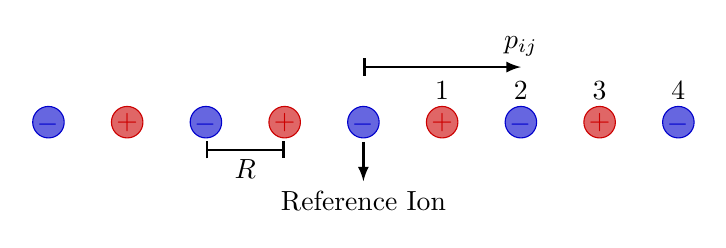
\begin{tikzpicture}
            \foreach \x in {-2, 0, ..., 4} {
                \draw[positive red, fill=positive red!60] (\x, 0) circle [radius=0.2cm];
                \node[positive red] at (\x, 0) {\(+\)};
                \draw[negative blue, fill=negative blue!60] (\x + 1, 0) circle [radius=0.2cm];
                \node[negative blue] at (\x - 0.01 + 1, -0.03) {\(-\)};
            }
            \draw[negative blue, fill=negative blue!60] (-3, 0) circle [radius=0.2cm];
            \node[negative blue] at (-3 - 0.01, 0 - 0.03) {\(-\)};
            \draw[->, thick] (1, -0.25) -- ++ (0, -0.5) node[below] {Reference Ion};
            \draw[|-|, thick] (-1, -0.35) -- (0, -0.35) node[midway, below] {\(R\)};
            \foreach \i in {1, ..., 4} {
                \node at (1 + \i, 0.4) {\i};
            }
            \draw[|->, thick] (1, 0.7) -- ++ (2, 0) node[above] {\(p_{ij}\)};
        \end{tikzpicture}
        \caption[One-dimensional ionic crystal.]{One-dimensional crystal of alternating positive and negative ions.}
        \label{fig:1d ionic crystal}
    \end{figure}
    
    Computing the Madelung constant in higher dimensions is more tricky.
    As a start point summing in order of nearest neighbours doesn't work very well since the terms will oscillate from positive to negative.
    A better method is to sum over spherical shells.
    The resulting sum is conditionally convergent, and when it does converge it doesn't do so particularly quickly since the Coulomb potential goes as \(1/r\) and the number of ions in a spherical shell of radius \(r\) goes as \(r^2\).
    Fortunately we know that \ce{NaCl}, and other structures, exist and therefore we can assume that the sum converges.
    
    A better method for calculating the Madelung constant is the Ewald method.
    It involves transforming the sum to Fourier space for the calculation, and it turns out the convergence is much quicker in Fourier space.
    This method is used by most modern programs for crystal structure calculations.
    
    \subsection{Different Ionic Crystals}
    So far we have considered only \ce{NaCl}, and other crystals of a similar form.
    There are various ionic crystal structures, we typically identify these structures by the most common example.
    The three most common ionic crystal structures are the rock salt type, of which \ce{NaCl} is an example, caesium chloride type, \ce{CsCl}, and zinc blende, \ce{ZnS}.
    
    One scheme for crystal naming is the \define{\textit{Struktubericht} symbols}\index{Struktubericht symbols@\textit{Struktubericht} symbols}.
    In this scheme \(\mathrm{A}\) refers to crystals of a single atom, \(\mathrm{B}\) to crystals of two elements in an equal ratio, \(\mathrm{C}\) to crystals of two elements in a two-to-one ratio, and \(\mathrm{D})\) for all other stoichiometry.
    As well as this there is a number.
    So \(\mathrm{A1}\) is FCC, \(\mathrm{A2}\) is BCC, \(\mathrm{A3}\) is HCP.
    However, we are interested in ionic crystals of equal stoichiometry, so \(\mathrm{B}\).
    Rock salt is of type \(\mathrm{B1}\), \ce{CsCl} is of type \(\mathrm{B2}\), and \ce{ZnS} is of type \(\mathrm{B3}\).
    See \cref{fig:common ionic crystal structures}.
    
    \begin{figure}
        \begin{subfigure}{0.6\textwidth}
            \centering
            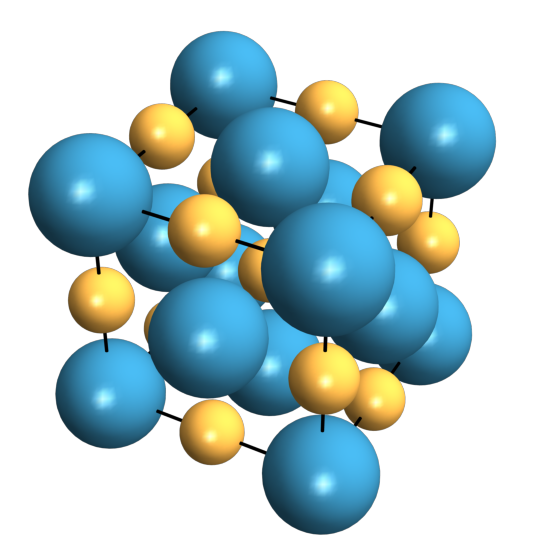
\includegraphics[width=0.6\textwidth]{images/rocksalt.pdf}
            \caption[Rock salt structure.]{The rock salt (\(\mathrm{B1}\)) structure.}
        \end{subfigure}
        \begin{subfigure}{0.6\textwidth}
            \centering
            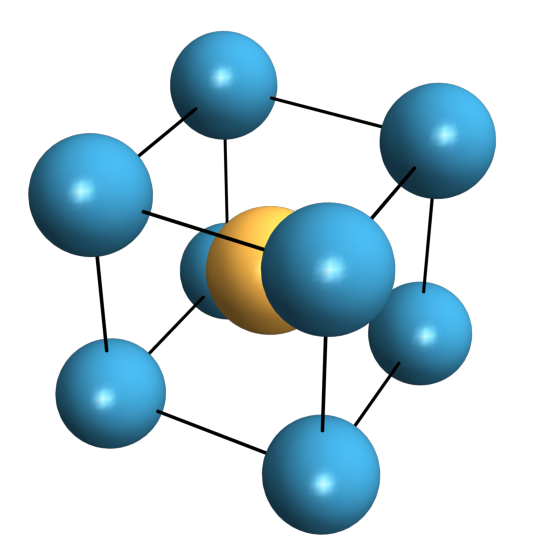
\includegraphics[width=0.6\textwidth]{images/CsCl.pdf}
            \caption[Caesium chloride structure.]{The caesium chloride (\(\mathrm{B2}\)) structure.}
        \end{subfigure}
        \begin{subfigure}{0.6\textwidth}
            \centering
            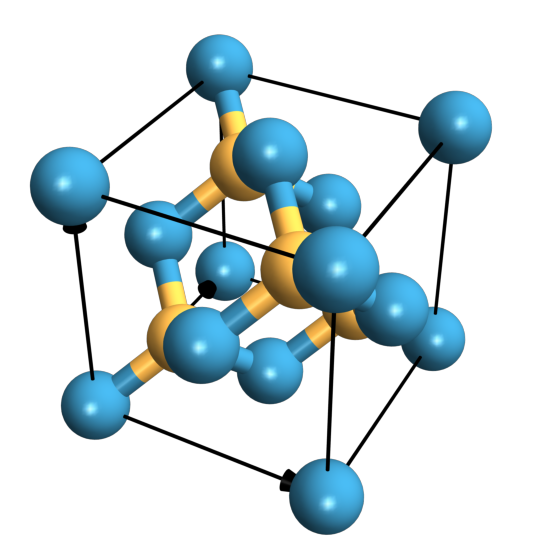
\includegraphics[width=0.6\textwidth]{images/ZnS1.pdf}
            \caption[Zinc blende structure.]{The zinc blende (\(\mathrm{B3}\)) structure.}
        \end{subfigure}
        \begin{subfigure}{0.6\textwidth}
            \centering
            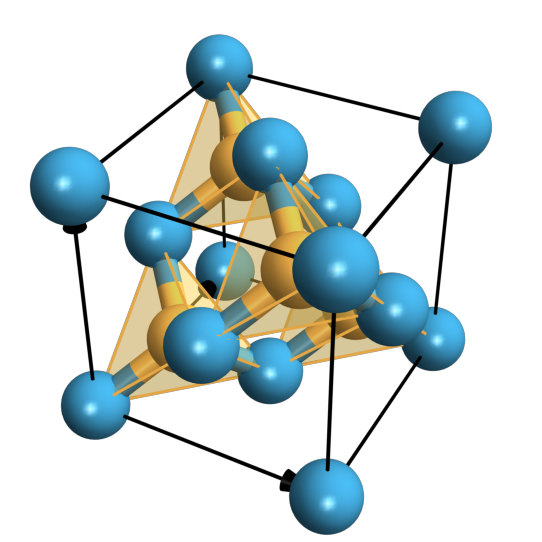
\includegraphics[width=0.6\textwidth]{images/ZnS2.pdf}
            \caption[Zinc blende structure.]{The zinc blende (\(\mathrm{B3}\)) structure.}
        \end{subfigure}
        \caption[Common ionic crystal structures.]{The three most common ionic crystal structures, the rock salt, \ce{CsCl}, and \ce{ZnS} types, also known as \(\mathrm{B1}\), \(\mathrm{B2}\), and \(\mathrm{B3}\).}
        \label{fig:common ionic crystal structures}
    \end{figure}
    
    In all three of these structures both ions have the same local environment.
    That is, each ion is surrounded by the other ion in the same way such that if you swapped the ions the crystal wouldn't change.
    Ions of a similar size tend to form the \ce{CsCl} type whereas ions with a larger size difference tend to form the rock salt type.
    
    The \ce{ZnS} structure is the same as diamond but if you replaced half of the atoms in diamond with a different type.
    This structure is common amongst semiconductors used in optoelectronics (such as LEDs\glossary[acronym]{LED}{light emitting diode}), such as \ce{GaAs}, \ce{GaN}, and \ce{GaP}.
    This type of structure is often found in materials with mixed ionic and covalent bonding.
    
    \subsection{Ionic Spacing}
    We can find the equilibrium spacing between ions by finding the value of \(R\) which minimises \(U_{\tot}\).
    To do so we need to choose a repulsive potential, we choose \(V_{\mathrm{r}}(R) = \lambda\e^{-R/\rho}\).
    We then have
    \begin{equation}
        0 = \diff{U_{\tot}}{R}[R=R_0] = N\left[ -\frac{z\lambda}{\rho}\e^{-R_0/\rho} + \alpha\frac{q^2}{4\pi\varepsilon_0R_0^2} \right].
    \end{equation}
    Rearranging this we have
    \begin{equation}
        \left( \frac{R_0}{\rho} \right)^{2} \e^{-R_0/\rho} = \frac{1}{4\pi\varepsilon_0}\frac{\alpha q^2}{\rho z\lambda}.
    \end{equation}
    This has no analytic solution.
    Numerical solutions give \(R_0/\rho \approx 10\).
    Notice that making either \(\alpha\) or \(q\) larger will make the crystal denser.
    The equilibrium energy is
    \begin{equation}
        U_{\tot}(R_0) = -N\alpha\frac{q^2}{4\pi\varepsilon_0R_0}\left( 1 - \frac{\rho}{R_0} \right).
    \end{equation}
    
    As an example consider \ce{KCl}.
    This has the rock salt structure type with \(z = 6\).
    Experimental properties of \ce{KCl} can be reproduced with \(\rho = \qty{0.30}{\angstrom}\) and \(\lambda = \qty{4}{\kilo\electronvolt}\).
    We then find \(R_0 \approx 10\rho = \qty{3}{\angstrom}\).
    
    \section{Covalent Crystals}
    Covalent bonding arises when the atomic wave functions overlap in such a way as to minimise the energy.
    Crudely we think of this as \enquote{sharing electrons}.
    Unlike other bonding types this forms directional bonds.
    
    Covalent bonding is more complicated to describe so, rather than give a full quantum mechanical description, we will simply make an analogy to the bonding of the \ce{H_2} molecule\footnote{see the notes from principles of quantum mechanics course.}.
    When two hydrogen atoms are brought together their initial atomic, \(\mathrm{1s}\), wave functions are no longer eigenstates.
    Instead, a new, lower energy, bonding molecular orbital, \(\mathrm{\upsigma_{1s}}\), is formed, as well as a higher energy, anti-bonding molecular orbital, \(\mathrm{\upsigma_{1s}^*}\).
    See \cref{fig:MO H2}.
    The bonding state has anti-parallel spins and a symmetric wave function, for this reason it is sometimes referred to as an S state.
    The anti-bonding state has parallel spins and an antisymmetric wave function, for this reason it is sometimes referred to as an A state.
    For a covalently bonded molecule to be stable the energy must decrease when the wave functions overlap.
    For this reason \ce{H_2} is stable but \ce{He_2} is not, since the electrons in the anti-bonding state increase the energy by as much as the electrons in the bonding state decrease it.
    
    \begin{figure}
        \tikzexternaldisable
        \begin{modiagram}
            \atom{left} {1s = {0}}
            \atom{right} {1s = {0}}
            \molecule{1sMO = 0.75; pair}
            \node[left] at ($(1sleft) + (-0.1, 0)$) {\(\mathrm{1s}\)};
            \node[right] at ($(1sright) + (0.1, 0)$) {\(\mathrm{1s}\)};
            \node[below] at ($(1sigma) + (0, -0.1)$) {\(\mathrm{\upsigma_{1s}}\)};
            \node[above] at ($(1sigma*) + (0, 0.1)$) {\(\mathrm{\upsigma_{1s}^*}\)};
            \node[above] at ($(1sigma*) + (0, 1)$) {\ce{H_2}};
        \end{modiagram}
        \begin{modiagram}
            \atom{left} {1s = {0}}
            \atom{right} {1s = {0}}
            \molecule{1sMO = 0.75; pair}
            \node at (3, 0.75) {\(\upharpoonleft\mkern-5mu\downharpoonright\)};
            \node[left] at ($(1sleft) + (-0.1, 0)$) {\(\mathrm{1s}\)};
            \node[right] at ($(1sright) + (0.1, 0)$) {\(\mathrm{1s}\)};
            \node[below] at ($(1sigma) + (0, -0.1)$) {\(\mathrm{\upsigma_{1s}}\)};
            \node[above] at ($(1sigma*) + (0, 0.1)$) {\(\mathrm{\upsigma_{1s}^*}\)};
            \node[above] at ($(1sigma*) + (0, 1)$) {\ce{H_2^{2-}}};
        \end{modiagram}
        \tikzexternalenable
        \caption[Molecular orbital diagrams for \ce{H_2} and \ce{He_2}]{Molecular orbital diagrams for \ce{H_2} and \ce{He_2}.}
        \label{fig:MO H2}
    \end{figure}

    \section{Metallic Crystals}
    Metallic bonds are basically more extreme forms of covalent bonds in which the overlap of all wave functions (not just neighbours like in covalent bonds) decrease the energy to form a stable state.
    The valence electrons become delocalised.
    The bonds in a metal are non-directional, unlike covalent bonds.
    We will give a fuller picture later where we treat the delocalised electrons like a Fermi gas.
    
    \section{Mixed Binding}
    So far we have only considered one type of bonding at a time.
    In reality all types of bondings occur at once.
    Van der Waaals bonding is weak enough that most of the time it is negligible compared to the other bonding types.
    The refractory metals (a subset of the d-block transition metals including \ce{Mo} and \ce{W}) have high melting points and hardness since they are a mix of metallic and covalently bonded.
    Many metal-non-metal crystals mix covalent and ionic bonding in various amounts, ranging from almost pure covalent bonding for \ce{Si} to about one third ionic bonding for \ce{GaAs}, to two thirds for \ce{ZnS}, to almost pure ionic for \ce{NaCl}.
    
    One interesting case of mixed bonding is graphite.
    In graphite carbon, which is usually \(\mathrm{1s^22s^22p^4}\), forms \(\mathrm{1s^22s^22p^2}\) valence electrons an \(\mathrm{sp^2}\) hybrid orbitals (covalent bonding) and a delocalised electrons (metallic bonding).
    This holds together layers of graphite.
    Between the layers the main bonding effect is van der Waals bonding.
    This leads to graphites interesting properties like being very conductive along the layers but not across and individual layers being strong but still being soft over all as the layers can easily move past each other.
    
    \chapter{Phonons}
    So far we have considered the atoms in a crystal to be stationary at their equilibrium positions, given by minimising the binding energy.
    We saw, for example, that for helium at low temperature, the vibrational energy of the atoms can effect the physical properties, even to the extent that helium doesn't for a crystal structure at \qty{0}{\kelvin} and standard pressure.
    
    One of the most important quantities that for which we need to take atomic vibrations into account is the heat capacity.
    We will see three models of heat capacity in increasing complexity and accuracy.
    Along the way we will introduce the idea of phonons and look at some other consequences.
    
    \section{Heat Capacity}
    \subsection{Classical Heat Capacity}
    Recall that the heat capacity is defined as the rate of change of internal energy, \(U\), with respect to the temperature, \(T\):
    \begin{equation}
        \heatCapacityVolume \coloneqq \diffp{U}{T}[V].
    \end{equation}
    Strictly the definition above is the heat capacity at constant volume, but, for solids the heat capacity at constant pressure, \(\heatCapacityPressure\), is very similar.
    Since the change in volume as a solid is heated is relatively small compared to a gas.
    So we usually treat the two as the same.
    To measure the heat capacity we take a sample of the material, heat it, and measure the corresponding temperature change.
    
    For a monatomic ideal gas the heat capacity is \(\heatCapacityVolume = 3\boltzmann/2\) per atom, or \(\heatCapacityVolume = 3\boltzmann\avogadro/2 = 3R/2\) per mole, where \(R\) is the gas constant.
    In general the gas has a heat capacity of \(\boltzmann/2\) per quadratic degree of freedom per atom, and we assume that only translational degrees of freedom are accessible at low temperatures.
    
    For solids the positions of atoms are fixed.
    Instead the atoms can vibrate about their equilibrium positions.
    This gives six degrees of freedom, two for each Cartesian direction, one kinetic and one potential.
    This suggests a heat capacity of \(C = 3\boltzmann\) per atom.
    This is the \defineindex{Dulong--Petit law}, it suggests a constant, positive heat capacity.
    
    The problem is that experimentally at low temperatures the Dulong--Petit law doesn't hold.
    In fact we find that \(C \to 0\) as \(T \to 0\).
    
    \subsection{Einstein Model}
    In this section we summarise the \defineindex{Einstein model} of the heat capacity\footnote{for more details see the notes on statistical mechanics from the thermal physics course}.
    In this model we treat each atom as being close to its equilibrium position.
    This allows us to Taylor expand the potential.
    Since the equilibrium is a minimum the first derivative vanishes and we are left with a quadratic potential, up to an unimportant constant term, given by \(V(\vv{\Delta r}) = C\Delta r^2/2\).
    \begin{wrn}
        The \(C\) here is \emph{not} the heat capacity, it's a force constant.
        Unfortunately the common alternative of \(k\) clashes with the wave vector and so we are left with no good notation for this quantity.
        Fortunately the force constant doesn't appear in future calculations so this shouldn't be too much of an issue.
    \end{wrn}

    We then treat the atoms as quantum harmonic oscillators, in particular we assume they oscillate independently in three dimensions.    
    The energy levels of a one-dimensional harmonic oscillator are
    \begin{equation}
        E_n = \hbar\omega\left( n + \frac{1}{2} \right)
    \end{equation}
    where \(n \in \naturals\).
    The average value of \(n\) at temperature \(T\) is given by the Planck distribution function:
    \begin{equation}
        \expected{n} = \frac{1}{\e^{\hbar\omega\beta} - 1}
    \end{equation}
    where \(\beta \coloneqq 1/(\boltzmann T)\).
    The internal energy is then given by
    \begin{equation}
        U = 3N\hbar\omega_{\einstein}\left( \expected{n} + \frac{1}{2} \right)
    \end{equation}
    where the factor of 3 comes from considering three-dimensional oscillators.
    Here \(\omega_{\einstein} = \sqrt{C/m}\) is a parameter that depends on the material with \(m\) being the mass of an atom.
    
    The heat capacity can then be found by differentiating:
    \begin{align}
        C &= \diffp{U}{T}\\
        &= 3N\hbar\omega_{\einstein} \diffp{}{T}\left( \frac{1}{\e^{\hbar\omega_{\einstein}/\boltzmann T} - 1} + \frac{1}{2} \right)\\
        &= 3N\boltzmann \left( \frac{\hbar\omega_{\einstein}}{\boltzmann T} \right)^2 \frac{\e^{\hbar\omega_{\einstein}\beta}}{(\e^{\hbar\omega_{\einstein}\beta} - 1)^2}.
    \end{align}
    This has only a single parameter, \(\omega_{\einstein}\), which is more commonly given in terms of the \defineindex{Einstein temperature}, \(\Theta_{\einstein} \coloneqq \hbar\omega_{\einstein}/\boltzmann\).
    This model definitely improves on the Dulong--Petit law.
    In particular \(C \to 0\) as \(T \to 0\).
    However, the model still fails to match real data at low temperatures typically giving values of the heat capacity that are too low.
    This is a fundamental issue with the model due to the assumption of independent oscillators, which is simply not valid, particularly at low temperatures.
    
    For a better model we will need to study vibrations of atoms more carefully, and this is what we do in the rest of this chapter.
    
    \begin{figure}
        \tikzsetnextfilename{einstein-model-prediction}
        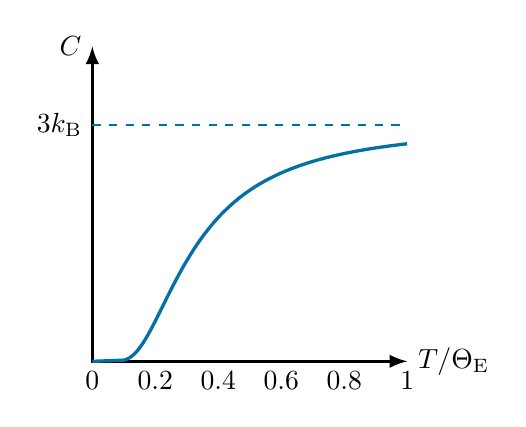
\begin{tikzpicture}
            \draw[very thick, <->] (4, 0) node[right] {\(T/\Theta_{\einstein}\)} -- (0, 0) -- (0, 4) node[left] {\(C\)};
            \draw[highlight, very thick] (0, 0) .. controls (0.2, 0.002) .. (0.41, 0.015);  % bodge near zero as precision too low
            \draw[highlight, very thick, domain=0.4:4, samples=200] plot (\x, {3/(\x^2/4*sinh(2/(\x))^2)});
            \draw[highlight, dashed, thick] (0, 3) node[left, black] {\(3\boltzmann\)} -- (4, 3);
            \foreach \i in {0, 0.2, 0.4, 0.6, 0.8, 1} {
                \node at (4*\i, -0.25) {\i};
            }
        \end{tikzpicture}
        \caption[Heat capacity predicted by Einstein model.]{The heat capacity as predicted by the Einstein model.}
    \end{figure}
    
    \section{Phonons in One Dimension}
    Consider a chain of atoms, all of the same type, of mass \(M\), spaced \(a\) apart and joined to their neighbours by springs with force constant \(C\).
    The atoms typically move a distance \qtyrange{0.05}{0.1}{\angstrom} from their equilibrium positions, that is approximately \qty{2}{\percent} of the interatomic separation.
    
    \begin{figure}
        \tikzsetnextfilename{monatomic-chain}
        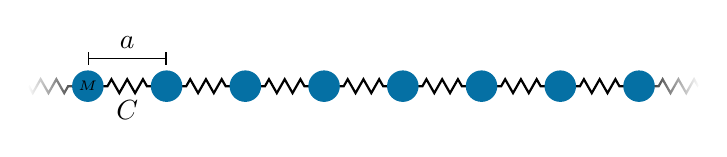
\begin{tikzpicture}
            \foreach \i in {0, 1, ..., 6} {
                \draw[thick, decorate, decoration={zigzag, post length=0.25cm, pre length=0.25cm, segment length=0.2cm}] (\i, 0) -- ++ (1, 0);
            }
            \draw[thick, decorate, decoration={zigzag, pre length=0.25cm, segment length=0.2cm}, path fading=west] (0, 0) -- ++ (-0.75, 0);
            \draw[thick, decorate, decoration={zigzag, pre length=0.25cm, segment length=0.2cm}, path fading=east] (7, 0) -- ++ (0.75, 0);
            \foreach \i in {0, 1, ..., 7} {
                \fill[highlight] (\i, 0) circle [radius = 0.2cm];
            }
            \node at (0.5, -0.3) {\(C\)};
            \draw[|-|] (0, 0.35) -- ++ (1, 0) node[midway, above] {\(a\)};
            \node at (0, 0) {\tiny\(M\)};
        \end{tikzpicture}
        \caption[One-dimensional chain of atoms.]{A chain of a single type of atom of mass \(M\), separated at equilibrium by a distance \(a\), and connected to their neighbours by a spring with force constant \(C\).}
    \end{figure}
    
    For now we consider only the interactions between nearest neighbours.
    Let \(u_s\) be the displacement of the \(s\)th atom.
    Then the force on this atom is
    \begin{equation}
        F_s = C(u_{s+1} - u_s) + C(u_{s-1} - u_s) = C(u_{s+1} + u_{s-1} - 2u_s)
    \end{equation}
    where the first term corresponds to the force due to the relative separation of atoms \(s\) and \(s + 1\) from their equilibrium separation, and the second term corresponds to \(s\) and \((s - 1)\)'s relative positions.
    The equation of motion for atom \(s\) is
    \begin{equation}\label{eqn:1d phonon eom}
        M\diff[2]{u_s}{t} = C(u_{s+1} + u_{s-1} - 2u_s).
    \end{equation}
    We make an ansatz of wavelike solutions:
    \begin{equation}
        u_s(t) = u\e^{i(Ksa - \omega t)}
    \end{equation}
    where \(K\) is the wave vector, which relates to the wavelength by \(\lambda = 2\pi/K\), \(u\) is the amplitude of the wave, and \(\omega\) is the (angular) frequency of the wave.
    Atom \(s\) is at equilibrium position \(x = sa\), taking the zeroth atom's equilibrium position as \(x = 0\).
    
    Differentiating the ansatz we have
    \begin{align*}
        u_s'(t) &= -i\omega u\e^{i(Ksa - \omega t)} = -i\omega u_s(t),\\
        u_s''(t) &= -\omega^2u\e^{i(Ksa - \omega t)} = -\omega^2 u_s(t).
    \end{align*}
    We can also apply the ansatz for \(u_{s+1}\) and \(u_{s-1}\) getting
    \begin{align}
        u_{s+1} &= u\e^{i(K[s+1]a - \omega t)} = u\e^{i(Ksa - \omega t)}\e^{iKa} = \e^{iKa}u_s,\\
        u_{s-1} &= u\e^{i(K[s-1]a - \omega t)} = u\e^{i(Ksa - \omega t)}\e^{-iKa} = \e^{-iKa}u_s.
    \end{align}
    Substituting the ansatz into \cref{eqn:1d phonon eom} we get
    \begin{equation}
        -M\omega^2 u_s = Cu_s(\e^{iKa} + \e^{-iKa} - 2) = Cu_s[\cos(Ka) - 2].
    \end{equation}
    From this we get
    \begin{equation}
        \omega^2 = \frac{2C}{M}[1 - \cos(Ka)] = \frac{4C}{M}\sin^2\left( \frac{1}{2}Ka \right).
    \end{equation}
    Which gives
    \begin{equation}
        \omega = 2\sqrt{\frac{C}{M}} \abs*{\sin\left( \frac{1}{2}Ka \right)}
    \end{equation}
    This is the \defineindex{phonon dispersion relation}, it relates the frequency and wave vector.
    It is periodic in \(K\), with an infinite number of solutions for \(K\) for each \(\omega\).
    However, only the wave vectors with \(\abs{K} \le \pi/a\) are physically meaningful.
    All other wave vectors can be reduced to a wave vector in this range by addition on \(2\pi n/a\), for some \(n \in \integers\).
    We call the region of physically meaningful wave vectors the first \defineindex{Brillouin zone}.
    
    \section{Wigner--Seitz Cells}\label{sec:wigner-seitz cells}
    The \defineindex{Wigner--Seitz construction} is a way to define a unique primitive unit cell.
    The unit cells defined aren't very useful in real space as they cannot be described by three lattice vectors.
    However, they are still valid unit cells since they tile to fill space in a periodic way with no gaps.
    
    The construction is as follows:
    \begin{enumerate}
        \item Connect a chosen central lattice point to all nearby lattice points.
        \item Draw planes perpendicular through the midpoints of all connecting lines.
        \item The smallest volume enclosed by these planes is the Wigner--Seitz cell.
    \end{enumerate}
    This is demonstrated in two dimensions in \cref{fig:wigner-seitz}.
    \Cref{fig:wigner-seitz tiles plane} then shows how this same cell tiles the plane and contains a single lattice point, making it a valid primitive unit cell.
    
    The main use of Wigner--Seitz cells is to define the Brillouin zone as the Wigner--Seitz cell in reciprocal space.
    For example the reciprocal lattice of FCC is BCC and the Wigner--Seitz cell of a BCC lattice is the Brillouin zone for the FCC lattice.
    
    \section{Phonons in Three Dimensions}
    While treating coupled oscillation in three dimensions is somewhat more complicated the results are fundamentally the same as in one dimension.
    This is because three-dimensional travelling waves represent movement of whole crystal layers.
    Instead of a single chain oscillating we have multiple chains oscillating in parallel.
    If the direction of travel isn't along one of the lattice vectors then we can still decompose the motion into waves along the lattice vectors.
    
    The main difference in three dimensions is that the force constant, \(C\), will usually depend on the direction of the wave vector, \(\vv{K}\), since crystals are, in general, not isotropic.
    
    It is possible to calculate phonon dispersion relations from first principles from the electronic structure.
    This is done using a computational framework called \defineindex{density functional theory} (DFT)\glossary[acronym]{DFT}{density functional theory}.
    It allows for a good approximation to the many-electron quantum mechanical description of the crystal.
    
    \begin{figure}
        \tikzsetnextfilename{wigner-seitz-construction}
        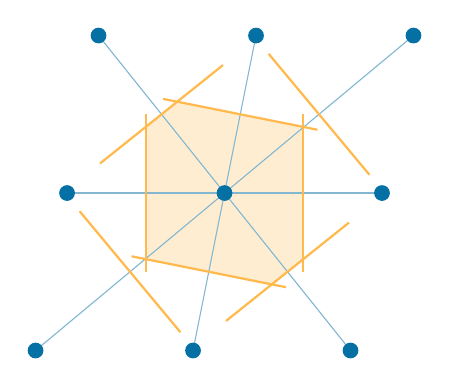
\begin{tikzpicture}
            \coordinate (00) at (0, 0);
            \coordinate (10) at (2, 0);
            \coordinate (20) at (4, 0);
            \coordinate (01) at (0.4, 2);
            \coordinate (11) at (2.4, 2);
            \coordinate (21) at (4.4, 2);
            \coordinate (02) at (0.8, 4);
            \coordinate (12) at (2.8, 4);
            \coordinate (22) at (4.8, 4);
            
            \coordinate (1) at (1.4, 1.15);
            \coordinate (2) at (1.4, 2.825);
            \coordinate (3) at (1.8, 3.15);
            \coordinate (4) at (3.4, 2.85);
            \coordinate (5) at (3.4, 1.15);
            \coordinate (6) at (3, 0.825);
            
            \fill[complementary!25] (1) --(2) -- (3) -- (4) -- (5) -- (6) -- cycle;
            
            \draw[highlight!50] (00) -- (22);
            \draw[highlight!50] (02) -- (20);
            \draw[highlight!50] (01) -- (21);
            \draw[highlight!50] (10) -- (12);
            
            \foreach \i in {00, 10, 20, 01, 21, 02, 12, 22} {
                \coordinate (M) at ($(\i)!0.5!(11)$);
                \draw[complementary, thick] ($(M)!1cm!270:(\i)$) -- ($(M)!1cm!90:(\i)$);
            }
            
            \foreach \i in {00, 10, 20, 01, 11, 21, 02, 12, 22} \fill[highlight] (\i) circle [radius = 0.1cm];
        \end{tikzpicture}
        \caption[Wigner--Seitz cell.]{The Wigner--Seitz construction of a primitive unit cell.}
        \label{fig:wigner-seitz}
    \end{figure}

    \begin{figure}
        \tikzsetnextfilename{wigner-seitz-tile-plane}
        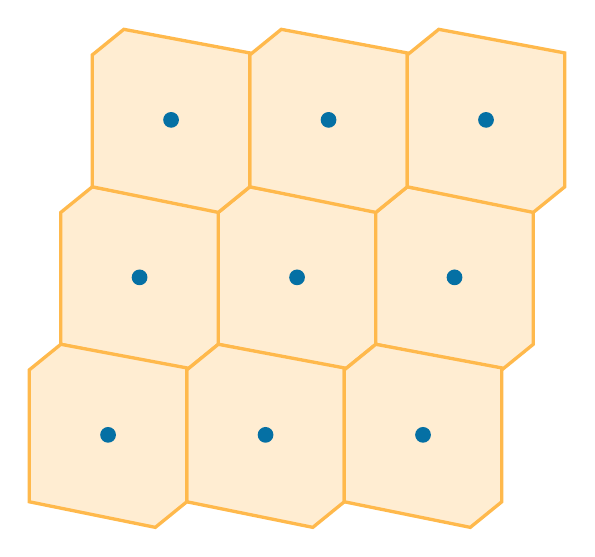
\begin{tikzpicture}
            \coordinate (00) at (0, 0);
            \coordinate (10) at (2, 0);
            \coordinate (20) at (4, 0);
            \coordinate (01) at (0.4, 2);
            \coordinate (11) at (2.4, 2);
            \coordinate (21) at (4.4, 2);
            \coordinate (02) at (0.8, 4);
            \coordinate (12) at (2.8, 4);
            \coordinate (22) at (4.8, 4);
            
            \coordinate (1) at (1.4, 1.15);
            \coordinate (2) at (1.4, 2.825);
            \coordinate (3) at (1.8, 3.15);
            \coordinate (4) at (3.4, 2.85);
            \coordinate (5) at (3.4, 1.15);
            \coordinate (6) at (3, 0.825);
            
            
            \draw[complementary, very thick, fill=complementary!25] (1) --(2) -- (3) -- (4) -- (5) -- (6) -- cycle;
            \foreach \i in {{2, 0}, {-2, 0}, {-0.4, -2}, {1.6, -2}, {-2.4, -2}, {0.4, 2}, {-1.6, 2}, {2.4, 2}} {
                \draw[complementary, very thick, fill=complementary!25, xshift=2cm] ($(1) + (\i)$) --($(2) + (\i)$) -- ($(3) + (\i)$) -- ($(4) + (\i)$) -- ($(5) + (\i)$) -- ($(6) + (\i)$) -- cycle;
            }
            
            \foreach \i in {00, 10, 20, 01, 11, 21, 02, 12, 22} \fill[highlight] (\i) circle [radius = 0.1cm];
        \end{tikzpicture}
        \caption[Wigner--Seitz cell tiles the plane]{A Wigner--Seitz cell is a primitive unit cell, meaning it contains one lattice point and tiles space, as shown here.}
        \label{fig:wigner-seitz tiles plane}
    \end{figure}
    
    When discussing Brillouin zones it is conventional to label lines of symmetry with capital Greek letters, and points of symmetry with capital Latin letters.
    The one exception is that the Brillouin zone centre, that is \(\vv{K} = \vv{0}\), is always denoted \(\Gamma\).
    
    \begin{figure}
        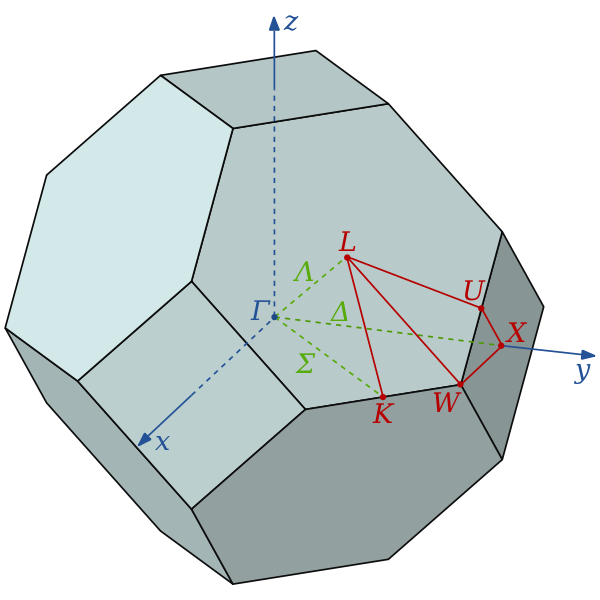
\includegraphics[width=0.8\textwidth]{images/brilloin-zone-fcc.png}
        \caption[3D Brillouin zone]{The first Brillouin zone for an FCC crystal. The Brillouin zone centre is labelled \(\Gamma\) and the other labelled lines and points are of particularly high symmetry. Taken from \cite{Inductiveload2008}}
    \end{figure}

    To fully plot the dispersion relation would require four dimensions (three to represent \(\vv{k}\) and one for \(\omega\)).
    Instead we typically plot dispersion relations along a line in the Brillouin zone.
    This is fine since typically we can choose a line such that it goes through all of the interesting points.
    An example is shown in \cref{fig:dispersion relation in brillouin zone}.
    Note that it is conventional to work with frequencies (as opposed to angular frequencies) with phonons, typically phonons range in frequency from \qty{100}{\hertz} to \qty{10}{\tera\hertz}.
    
    \begin{figure}
        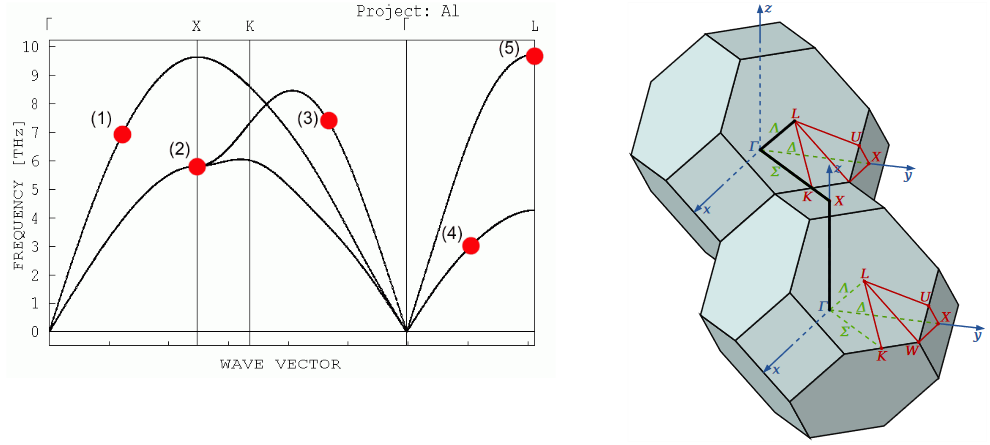
\includegraphics[width=0.8\textwidth]{images/dispersion-relation-brillouin-zone.png}
        \caption[Dispersion relation]{Dispersion relation for a sample of FCC aluminium. The dispersion relation is plotted travelling along the black line, starting in the lower Brillouin zone and ending in the equivalent, higher Brillouin zone. Notice that there is degeneracy between \(\Gamma\) and \(X\), as well as between \(\Gamma\) and \(L\), since we can only see two branches at these points. Taken from \cite{phonondispersionrelation}}
        \label{fig:dispersion relation in brillouin zone}
    \end{figure}
    
    In three dimensions atoms can oscillate in three orthogonal directions.
    Along the direction of propagation, giving longitudinal waves, or in along one of two perpendicular directions to the propagation, giving transverse waves.
    
    For a crystal structure with one atom in the primitive unit cell there are three phonon modes per wave vector, however, it is possible that they are degenerate.
    The longitudinal branch is usually the highest frequency and the transverse branches tend to be degenerate in high symmetry situations.
    
    \section{Energy Quantisation and Momentum}
    Consider a quantum harmonic oscillator with frequency \(\omega_{0}\).
    The energy levels are given by \(E_n = (n + 1/2)\hbar\omega_0\).
    We can treat the energy of our phonons similarly by substituting \(\omega_0\) for the dispersion relation, \(\omega(K)\).
    This gives energy levels
    \begin{equation}
        E_n(K) = \hbar\omega(K)\left( n + \frac{1}{2} \right) = \hbar\sqrt{\frac{4C}{M}}\left( n + \frac{1}{2} \right).
    \end{equation}
    
    We can only change the energy in steps of \(\omega(K)\).
    The total energy must be conserved so if a phonon of energy \(\hbar\omega\) is created in some process it must absorb energy \(\hbar\omega\) from the process.
    On the other hand if a phonon of energy \(\hbar\omega\) is destroyed in a process then its energy must be absorbed by other parts of the process.
    
    We can treat a phonon as a quantum of vibrational energy, \(\hbar\omega(K)\).
    The phonon also has well defined momentum, \(\hbar\vv{K}\).
    In this way the phonon is a bit like a particle.
    The phonon does \emph{not} have well defined position, it's a wave.
    This is different to particles.
    We therefore say that phonons are quasiparticles.
    
    The momentum of a phonon is not the same as the momentum in the mechanical sense.
    The momentum of a given atom will always be offset by the momentum of another particle oscillating exactly out of phase.
    However, we can still use ideas like momentum conservation.
    
    Consider an elastic scattering of a particle.
    If it starts with the initial wave vector, \(\vv{k_{\mathrm{i}}}\), and ends with the wave vector \(\vv{k_{\mathrm{f}}}\), then the crystal must recoil with momentum \(-\hbar\vv{G}\), where \(\vv{G}\) satisfies
    \begin{equation}
        \vv{k_{\mathrm{f}}} = \vv{k_{\mathrm{i}}} + \vv{G}.
    \end{equation}
    \(\vv{G}\) must be a reciprocal lattice vector with integer coefficients.
    This means that the momentum change is quantised.
    There are no phonons in this process.
    
    Consider an inelastic scattering of a particle.
    If a phonon is created in the process then we modify the previous equation to
    \begin{equation}
        \vv{k_{\mathrm{f}}} + \vv{K} = \vv{k_{\mathrm{i}}} + \vv{G},
    \end{equation}
    where \(\vv{K}\) is the wave vector of the phonon.
    Similarly if a phonon is destroyed in the process we modify it to
    \begin{equation}
        \vv{k_{\mathrm{f}}} = \vv{k_{\mathrm{i}}} + \vv{G} + \vv{K}.
    \end{equation}
    
    \section{Measuring Phonon Dispersion}
    We have only considered nearest neighbours when calculating phonon dispersion relations.
    Data has been collected that reveals that interactions up to the 10th nearest neighbours can be important enough to give measurable differences in dispersion relations.
    
    Phonon dispersion relations can be measured by measuring the momentum and energy change of scattered particles.
    Doing so for a variety of angles and initial momenta can allow us to work out possible energy and momentum changes, which can be used to work out the phonon dispersion relation.
    
    \section{Speed of Sound}
    Sound waves in solids are simply low frequency phonons, typically with frequency from a few hertz, up to a few million hertz.
    This is much lower than typically phonon energy which is a few terahertz.
    
    Recall that we have the dispersion relation
    \begin{equation}
        \omega^2(K) = \frac{2C}{M}[1 - \cos(Ka)].
    \end{equation}
    The \defineindex{speed of sound} is defined as the \defineindex{group velocity},
    \begin{equation}
        v_g \coloneqq \diff{\omega}{K}.
    \end{equation}
    Given the low frequency of sound waves the speed of sound corresponds to the slope of the dispersion relation near \(K = 0\) (which is the \(\Gamma\) point).
    We therefore have \(Ka \ll 1\), meaning that we can Taylor expand the \(\cos\) giving \(\cos(Ka) \approx 1 - K^2a^2/2\), which then simplifies the dispersion relation to
    \begin{equation}
        \omega^2(K) \approx\frac{C}{M} K^2a^2 \implies \omega(K) \approx \sqrt{\frac{C}{M}}aK.
    \end{equation}
    We see that this is linear in \(K\) and we can simply read off the derivative as
    \begin{equation}
        v_g \coloneqq \diff{\omega}{K} \approx a\sqrt{\frac{C}{M}}.
    \end{equation}
    From this we see that the speed of sound, \(v_{\sound} \coloneqq v_g \approx \omega/K = \nu \lambda\), where \(\nu = 2\pi\omega\) is the frequency and \(\lambda = 2\pi/K\) the wavelength.
    
    \section{Discrete Wave Vectors}
    Real heat capacity measurements at high temperature give an upper heat capacity of \(3R\).
    Our model does not.
    The thing we are missing is that real crystals have a finite size.
    This effects which phonon modes are possible, since the existence of boundaries gives us boundary conditions.
    
    \subsection{Boundary Conditions in One Dimension}
    Consider a chain of \(N + 1\) atoms with equilibrium separation \(a\), forming a one-dimensional crystal of length \(L = Na\).
    We can have wave solutions with nodes on the surface, i.e. standing waves.
    These have wavelength \(\lambda = 2L/n\).
    This corresponds to discrete allowed wave vectors
    \begin{equation}
        K = \frac{\pi n}{L}, \qqwhere n = 1, \dotsc, N - 1.
    \end{equation}
    
    Now suppose we take the same chain of atoms and bend it into a circle.
    This shouldn't change the physical properties, we've never observed the macroscopic geometry of a crystal effecting material properties.
    We can then impose periodic boundary conditions on this circular crystal.
    For simplicity we make the \((N + 1)\)th atom the first atom, so we have \(N\) atoms, and the circumference is \(L = Na\).
    The travelling wave solution is
    \begin{equation}
        u_s = u(0)\e^{i(sKa - \omega_Kt)}
    \end{equation}
    where \(u_s\) is the displacement of the atom in position \(s\).
    The phase at any one point must be unique, which means we must have \(u_s = u_{s + N}\).
    This gives the quantisation condition
    \begin{equation}
        K = \pm\frac{2\pi n}{L}, \qqwhere n = 0, \pm 1, \pm 2, \dotsc, \pm N.
    \end{equation}
    
    \subsection{Boundary Conditions in Two Dimensions}
    In two dimensions the crystal size is its area, which we take to be \(A = L_xL_y = N_xN_ya^2\), assuming a rectangular region of crystal with \(N_x\) atoms along the \(x\)-axis and \(N_y\) atoms along the \(y\)-axis.
    Taking the crystal to be periodic in both directions, giving the geometry of a torus, the allowed wave vectors are
    \begin{equation}
        (K_x, K_y) = (0, 0), \left( \pm \frac{2\pi}{L_x}, \pm \frac{2\pi}{L_y} \right), \dotsc, \left( \pm\frac{N_x\pi}{L_x}, \pm\frac{N_y\pi}{L_y} \right).
    \end{equation}
    This means that the density of allowed wave vectors is one allowed wave vector per area
    \begin{equation}
        \frac{2\pi}{N_xa}\frac{2\pi}{N_ya} = \frac{(2\pi)^2}{A}
    \end{equation}
    in reciprocal space.
    
    \subsection{Boundary Conditions in Three Dimensions}
    The crystal has volume \(V = L_xL_yL_z = N_xN_yN_za^3\), where we take a cuboidal crystal with edge lengths \(L_i = N_ia\), corresponding to \(N_i\) atoms.
    Taking periodic boundary conditions in all three directions, giving the geometry of a hyper-torus, we have allowed wave vectors
    \begin{equation}
        K_i = 0, \pm \frac{2\pi}{L_i}, \pm \frac{4\pi}{L_i}, \dotsc, \pm \frac{N\pi}{L_i}.
    \end{equation}
    There is one allowed wave vector per
    \begin{equation}
        \frac{(2\pi)^3}{V} = \frac{8\pi^3}{V}.
    \end{equation}
    
    \section{Phonon Density of States}
    Recall that the heat capacity is defined as
    \begin{equation}
        \heatCapacityVolume \coloneqq \diffp{U}{T}[V].
    \end{equation}
    At a given temperature \(T\) there will be a variety of phonon polarisations, \(p\), and wave vectors, \(\vv{K}\).
    The energy of any given phonon with polarisation \(p\) and wave vector \(\vv{K}\) is \(\hbar\omega_{\vv{K}, p}\), where the angular frequency, \(\omega_{\vv{K}, p}\), depends, in general, on both \(\vv{K}\) and \(p\).
    The total energy of all of these phonons is then
    \begin{equation}
        U = \sum_{\vv{K}}\sum_{p} U_{\vv{K}, p}
    \end{equation}
    where the sums are over all wave vectors and polarisations, and \(U_{\vv{K}, p}\) is the total energy of all phonons with wave vector \(\vv{K}\) and polarisation \(p\).
    We can replace \(U_{\vv{K}, p}\) with the energy of a single phonon with the same wave vector and polarisation, \(\hbar\omega_{\vv{K},, p}\), scaled by the fraction of phonons that have this energy, which is given by the Planck distribution:
    \begin{equation}
        \expected{n_{\vv{K}, p}} = \frac{1}{\e^{\hbar\omega_{\vv{K}, p}\beta} - 1},
    \end{equation}
    where \(\beta = 1/(\boltzmann T)\).
    Hence we have
    \begin{align}
        U &= \sum_{\vv{K}} \sum_{p} U_{\vv{K}, p}\\
        &= \sum_{\vv{K}} \sum_{p} \expected{n_{\vv{K}, p}} \hbar{\vv{K}, p}\\
        &= \sum_{\vv{K}} \sum_{p} \frac{\hbar\omega_{\vv{K}, p}}{\e^{\hbar\omega_{\vv{K}, p}\beta} - 1}.\label{eqn:phonon energy}
    \end{align}
    
    Importantly we only use \(\vv{K}\) and \(p\) as labels for the phonons, what actually matters are the energies, \(\hbar\omega_{\vv{K}, p}\), and the distribution of the energy.
    In particular the number of phonons with energies in the range \(\hbar\omega\) to \(\hbar(\omega + \Delta\omega)\) for some small \(\Delta\omega\).
    For this reason we use the density of states, \(D(\omega)\), which is such that \(\dl{N} = D(\omega) \dd{\omega}\), where \(\dl{N}\) is the change in the number of phonons associated with the frequency change \(\omega \to \omega + \dl{\omega}\).
    
    Integrating the density of states we have
    \begin{equation}
        N = \int\dl{N} = \int D(\omega) \dd{\omega}.
    \end{equation}
    So this gives the number of states in a given range.
    We can find the density of states by rearranging the definition to give
    \begin{equation}
        D(\omega) = \diff{N}{\omega}.
    \end{equation}
    For a given phonon dispersion relation, which we assume is isotropic so \(\omega(\vv{K}) = \omega(K)\), the density of states is
    \begin{equation}
        D(\omega) = \diff{N}{\omega} = \diff{N}{K} \diff{K}{\omega}.
    \end{equation}
    We can interpret \(\diff{N}/{K}\) as the density of states in reciprocal space, which can be found by considering the geometry of the space, and we can find the value of \(\diff{K}/{\omega} = (\diff{\omega}/{K})^{-1}\) from the dispersion relation.
    
    \subsection{Density of States in One Dimension}
    In one dimension there is one allowed wave vector per \(2\pi/L\), hence \(\diff{N}/{K}\), the number density of allowed states, is just the reciprocal of this:
    \begin{equation}
        \diff{N}{K} = \left( \frac{2\pi}{L} \right)^{-1} = \frac{L}{2\pi}.
    \end{equation}
    We get \(\diff{K}/{\omega}\) from \(1/(\diff{\omega}{K})\), which is the gradient of the dispersion relation.
    We therefore get a singularity when the dispersion relation is horizontal, which happens at the edge of the first Brillouin zone.
    
    \subsection{Density of States in Three Dimensions}
    In three dimensions there is one allowed wave vector per \(8\pi^3/V_{\mathrm{crystal}}\).
    Consider the a sphere in reciprocal space of radius \(K\).
    The volume of this sphere is
    \begin{equation}
        V_{\mathrm{sphere}}(K) = \frac{4}{3}\pi K^3.
    \end{equation}
    The number of states in this sphere is then
    \begin{equation}
        N_{\mathrm{sphere}}(K) = \frac{4}{3}\pi K^3 \left( \frac{8\pi^3}{V_{\mathrm{crystal}}} \right)^{-1} = \frac{K^3V_{\mathrm{crystal}}}{6\pi^2}.
    \end{equation}
    It follows that
    \begin{equation}
        \diff{N_{\mathrm{sphere}}}{K} = \frac{K^2V_{\mathrm{crystal}}}{2\pi^2}.
    \end{equation}
    The density of states is then
    \begin{equation}
        D(\omega) = \frac{K^2V_{\mathrm{crystal}}}{2\pi^2} \diff{K}{\omega}.
    \end{equation}
    
    We can do this same calculation in a slightly different way by considering spherical shells of radius \(K\) and thickness \(\dl{K}\).
    The volume of such a shell is
    \begin{equation}
        \dl{V_{\mathrm{shell}}(K)} = 4\pi K^2 \dl{K},
    \end{equation}
    which follows from
    \begin{align}
        \dd{V} &= \frac{4}{3}\pi^2 [(K + \dl{K})^3 - K^3]\\
        &= \frac{4}{3}\pi^2[K^3 + 3K^2\dd{K} + 3K\dd{K}^2 + \dd{K}^3 - K^2]\\
        &= 4\pi K^2 \dl{K} + \order(\dl{K}^2).
    \end{align}
    The number of states in the shell is 
    \begin{equation}
        \dl{N_{\mathrm{shell}}(K)} = 4\pi K^2\dd{K} \left( \frac{8\pi^3}{V_{\mathrm{crystal}}} \right)^{-1} + \order(\dl{K}^2) = \frac{K^2V_{\mathrm{crystal}}}{2\pi^2} \dl{K} + \order(\dl{K}^2).
    \end{equation}
    Hence the density of states is
    \begin{equation}
        \diff{N_{\mathrm{shell}}}{K} = \frac{K^2V_{\mathrm{crystal}}}{2\pi^2} + \order(\dl{K}),
    \end{equation}
    which is the same result as before in the limit \(\dl{K} \to 0\).
    
    In three dimensions there are significantly more stationary points in the dispersion relation, and hence poles in the density of states.
    The density of states quickly gets quite complicated, but treating such cases is beyond this course.
    
    \section{Heat Capacity}
    The heat capacity at constant volume is defined as
    \begin{equation}
        \heatCapacityVolume \coloneqq \diffp{U}{T}[V].
    \end{equation}
    The total energy of all phonons in the system, at some fixed temperature, \(T\), is characterised by the polarisation, \(p\), and wave vector, \(\vv{K}\), which give us the phonon energy, \(\hbar\omega_{\vv{K}, p}\).
    We saw in \cref{eqn:phonon energy} that the total energy stored in the lattice, that is the energy of the phonons, is
    \begin{equation}
        U_{\mathrm{lat}} = \sum_{\vv{K}} \sum_{p} \frac{\hbar\omega_{\vv{K}, p}}{\e^{\hbar\omega_{\vv{K}, p}\beta} - 1}.
    \end{equation}
    Using the density of states, \(D_p(\omega)\), of phonons of a given polarisation, \(p\), we find that
    \begin{equation}
        U_{\mathrm{lat}} = \sum_{p} \int_{0}^{\infty} D_p(\omega) \frac{\hbar\omega}{\e^{\hbar\omega\beta} - 1} \dd{\omega}.
    \end{equation}
    Now we have
    \begin{equation}
        \diffp{}{T} = \diffp{\beta}{T}\diffp{}{\beta} = -\frac{1}{\boltzmann T^2}\diffp{}{\beta}
    \end{equation}
    and so the lattice heat capacity is
    \begin{align}
        C_{\mathrm{lat}} &= -\frac{1}{\boltzmann T^2} \diffp{}{\beta} \sum_{p} \int_{0}^{\infty} D_p(\omega) \frac{\hbar\omega}{\e^{\hbar\omega\beta} - 1}\dd{\omega}\\
        &= \frac{1}{\boltzmann T^2} \sum_{p} \int_{0}^{\infty} D_p(\omega) \frac{(\hbar\omega)^2 \e^{\hbar\omega\beta}}{(\e^{\hbar\omega\beta} - 1)^2} \dd{\omega}\\
        &= \boltzmann \sum_p \int_{0}^{\infty} \int_0^{\infty} \frac{x^2\e^x}{(\e^x - 1)^2} \dd{\omega}
    \end{align}
    where \(x = \hbar\omega\beta\).
    
    \subsection{Einstein Model}
    In the Einstein model we have \(3N\) identical, uncoupled harmonic oscillators, all of frequency \(\omega_0\).
    This is equivalent to a density of states
    \begin{equation}
        D(\omega) = 3N\delta(\omega - \omega_0),
    \end{equation}
    and a single phonon branch.
    The heat capacity is then
    \begin{align}
        C_{\mathrm{lat}} &= \boltzmann \int_{0}^{\infty} 3N \delta(\omega - \omega_0) \frac{x^2\e^x}{(\e^x - 1)^2} \dd{\omega}\\
        &= 3N\boltzmann \left( \hbar\omega_0\beta \right)^2 \frac{\e^{\hbar\omega_0\beta}}{(\e^{\hbar\omega_0\beta} - 1)^2}.
    \end{align}
    As previously discussed this tends to the correct constant heat capacity at high temperatures and tends to zero as \(T \to 0\), but experimental data shows that at low temperatures the heat capacity should go as \(T^3\), which this doesn't.
    
    \subsection{Debye Model}\label{sec:debye model}
    The \defineindex{Debye model} manages to correctly encapsulate the \(T^3\) behaviour of the heat capacity at low temperatures, while still depending on only a single material parameter.
    It does so without us having to know the full phonon density of states.
    
    At low temperatures most phonon states are unattainable.
    The only states that can be occupied are the low energy, acoustic frequency, states.
    Here the dispersion relation is approximately linear.
    We imagine \(N\) oscillators in a crystal of volume \(V\) and a simplified dispersion relation, \(\omega(K) = vK\) where \(v\) is the sound velocity, since these low wave number phonons are exactly the phonons that form sound waves.
    Hence, \(K = \omega/v\).
    The density of states, in three dimensions, is then simply
    \begin{equation}
        D(\omega) = \frac{VK^2}{2\pi^2} \diffp{K}{\omega} = \frac{V\omega^2}{2\pi^2v^3}.
    \end{equation}
    
    One problem that we face is this doesn't correctly give us \(N\) when we integrate over all frequencies.
    To fix this we introduce a cut-off frequency, called the \define{Debye frequency}\index{Debye!frequency}, \(\omega_{\debye}\), which is such that
    \begin{equation}
        N = \int_0^{\omega_{\debye}} D(\omega) \dd{\omega}.
    \end{equation}
    This is a reasonable thing to do since in this model higher frequency states are largely unoccupied.
    Computing this integral we get
    \begin{equation}
        N = \int_{0}^{\omega_{\debye}} \frac{V\omega^2}{2\pi^2v^3} \dd{\omega} = \frac{V\omega_{\debye}^{3}}{6\pi^2v^3}
    \end{equation}
    from which we get
    \begin{equation}
        \omega_{\debye} = \left(6\pi^2v^3 \frac{N}{V}\right)^{1/3},
    \end{equation}
    which is useful since \(n = N/V\) is the number density, which is relatively easy to work out for a given material, we can simply consider the number of atoms in a unit cell and the volume of the unit cell.
    
    We can define the related quantity, the \define{Debye wave vector}\index{Debye!wave vector}, as
    \begin{equation}
        K_{\debye} \coloneqq \frac{\omega_{\debye}}{v} = \left( 6\pi^2\frac{N}{V} \right)^{1/3}.
    \end{equation}
    
    We are considering a three dimensional crystal, which will have three acoustic branches.
    Hence the phonon internal energy includes a factor of three and is given by
    \begin{equation}
        U = 3 \int_{0}^{\omega_{\debye}} D(\omega) \hbar\omega \expected{n(\omega)} \dd{\omega}
    \end{equation}
    where \(\expected{n(\omega)}\) is the Planck distribution, which means that \(\hbar\omega\expected{n(\omega)}\) is the average energy of an oscillator.
    Inserting the Debye density of states and the Planck distribution we have
    \begin{align}
        U &= 3\int_{0}^{\omega_{\debye}} \frac{V\omega^2}{2\pi^2v^3} \frac{\hbar\omega}{\e^{\hbar\omega\beta} - 1} \dd{\omega}\\
        &= \frac{3V\hbar}{2\pi^2v^3} \int_{0}^{\omega_{\debye}} \frac{\omega^3}{\e^{\hbar\omega\beta} - 1} \dd{\omega}.
    \end{align}
    
    We can express \(\omega_{\debye}\) in terms of the sound velocity, \(v\), and oscillator density, \(n = N/V\), which means that this form of the internal energy depends only on these two material parameters.
    We can calculate the heat capacity by computing the derivative:
    \begin{align}
        \heatCapacityVolume &= \diffp{U}{T}[V]\\
        &= -\frac{1}{\boltzmann T^2} \diffp{U}{\beta}[V]\\
        &= \frac{1}{\boltzmann T^2}\frac{3V\hbar}{2\pi^2v^3} \int_{0}^{\omega_{\debye}} \frac{\hbar\omega^4\e^{\hbar\omega\beta}}{(\e^{\hbar\omega\beta} - 1)^2} \dd{\omega}.
    \end{align}
    Introducing the dimensionless parameter \(x = \hbar\omega\beta\), and the \define{Debye temperature}\index{Debye!temperature} \(\vartheta_{\debye} = \hbar\omega_{\debye}/\boltzmann\) it can be shown that
    \begin{equation}
        \heatCapacityVolume = 9N\boltzmann \left( \frac{T}{\vartheta_{\debye}} \right)^{3} \int_{0}^{\vartheta_{\debye}/T} \frac{x^4\e^{x}}{(\e^{x} - 1)^2} \dd{x}.
    \end{equation}
    The prefactor of \(N\) shows that the heat capacity depends on the number of oscillators, that is the amount of material.
    This is a statement that the heat capacity is an extrinsic material, which we know, simply put \enquote{more stuff, more ability to store heat}.
    The only material parameter here is the Debye temperature, \(\vartheta_{\debye}\), which relates to the speed of sound and oscillator density by
    \begin{equation}
        \vartheta_{\debye} = v\frac{\hbar}{\boltzmann} \left( 6\pi^2 \frac{N}{V} \right)^{1/3}.
    \end{equation}
    The Debye temperature turns out to be a very useful material parameter, the heat capacity is related to the energy stored in phonons, which in turn depends on the strength of bonds, which relates to many other properties, such as the strength of the material.
    
    The most important feature of this equation for the heat capacity is its low temperature limit.
    It's not easy to figure out directly from this point though, instead we return to the internal energy, which we write as
    \begin{equation}
        U = \frac{3V}{2\pi^2v^3} \frac{\boltzmann^4T^4}{\hbar^3} \int_0^{x_{\debye}} \frac{x^3}{\e^x - 1} \dd{x}
    \end{equation}
    where \(x_{\debye} = \hbar\omega_{\debye}\beta\).
    We then can write this as
    \begin{equation}
        U = 9N\boltzmann T \left( \frac{T}{\vartheta_{\debye}} \right)^{3} \int_{0}^{\vartheta_{\debye}/T} \frac{x^3}{\e^x - 1} \dd{x}.
    \end{equation}
    
    In the limit of \(T \to \infty\) the upper limit of the integral goes to infinity.
    We then have my favourite integral, which it can be shown is
    \begin{equation}
        \int_{0}^{\infty} \frac{x^3}{\e^x - 1} \dd{x} = \frac{\pi^4}{15}.
    \end{equation}
    See \cref{app:integrals} for details.
    We then have
    \begin{equation}
        \heatCapacityVolume \approx \frac{12}{5} \pi^4N\boltzmann \left( \frac{T}{\vartheta_{\debye}} \right)^{3}
    \end{equation}
    which is proportional to \(T^3\), which agrees with experiments for most materials at low temperatures.
    
    \subsection{Beyond the Debye Model}
    The Einstein model has a delta distribution as a density of states.
    The Debye model improves on this with a density of states proportional to \(\omega^2\), and a cut-off frequency \(\omega_{\debye}\).
    There are many more approximations we can make (or not make) to get more accurate densities of states.
    They quickly become very complicated, and tend to be material specific.
    We'll stop with the Debye model as it is accurate enough for many purposes and still very general.
    
    \section{Diatomic Linear Chain}
    Many materials have a crystal structure with more than one atom per unit cell.
    We take as a model for such materials a chain of two alternating atoms with different masses, \(M_1\) and \(M_2\), forming a unit cell of length \(a\).
    This is the one dimensional analogue of materials like \ce{NaCl}.
    We consider only the interactions with nearest neighbours, which we take to form a harmonic potential with force constant \(C\).
    
    Nearest neighbours are always of alternating types, so we only need to consider one force constant for interactions between the two different types of atoms.
    The distance between nearest neighbours is \(a/2\), since the cell now repeats every two atoms.
    We index the atoms such that \(u_s\) is the position of one atom and \(v_s\) is the position of the next atom of the opposite type, and then \(u_{s+1}\) is the position of the next atom, back to the first type, and so on.
    We get two equations of motion:
    \begin{align}
        M_1 \diff[2]{u_s}{t} &= C(v_s + v_{s-1} - 2u_s),\\
        M_2 \diff[2]{v_s}{t} &= C(u_{s+1} + u_s - 2v_s).
    \end{align}
    Making the ansatz of travelling wave solutions,
    \begin{equation}
        u_s = u\e^{isKa}\e^{-i\omega t}, \qqand v_s = v\e^{isKa}\e^{-i\omega t},
    \end{equation}
    the first equation gives
    \begin{align}
        -M_1\omega^2u\e^{sKa}\e^{-i\omega t} &= C(v\e^{sKa} + v\e^{(s-1)Ka} - 2u\e^{sKa})\e^{-i\omega t}\\
        \implies -M_1\omega^2 &= Cv(1 + \e^{-Ka}) - 2u,
    \end{align}
    and similarly, for the second equation, we get
    \begin{equation}
        -\omega^2M_2v = Cu(\e^{iKa} + 1) - 2Cv.
    \end{equation}
    
    Given a set of homogeneous linear equations,
    \begin{equation}
        a u + b v = 0, \qqand cu + dv = 0,
    \end{equation}
    there is a non-trivial solution if and only if
    \begin{equation}
        \begin{vmatrix}
            a & b\\
            c & d
        \end{vmatrix}
        = ad - bc = 0.
    \end{equation}
    In our case this corresponds to the requirement that, for a non-trivial solution, we must have
    \begin{equation}
        \begin{vmatrix}
            2C - M_1\omega^2 & -C(1 + \e^{-iKa})\\
            -C(1 + \e^{iKa}) & 2C - M_2\omega^2
        \end{vmatrix}
        = 0
    \end{equation}
    from which we get
    \begin{equation}
        M_1M_2\omega^4 - 2C(M_1 + M_2)\omega^2 + 2C^2(1 - \cos(Ka)) = 0.
    \end{equation}
    This is quadratic in \(\omega^2\) with solutions
    \begin{equation}
        \omega^2 = \frac{2C(M_1 + M_2) \pm \sqrt{4C^2(M_1 + M_2)^2 - 8M_1M_2C^2(1 - \cos(Ka))}}{2M_1M_2}.
    \end{equation}
    This is plotted in \cref{fig:diatomic linear chain dispersion relation}.
    There are two positive solutions, which we refer to as branches.
    We call the higher frequency one the optical branch, as we will see these phonons are easily excited by visible light.
    We call the lower frequency the acoustic branch, as these phonons are responsible for sound waves.
    
    \begin{figure}
        \tikzsetnextfilename{diatomic-chain-dispersion-relation}
        \begin{tikzpicture}
            \tikzset{path text/.style={decoration={text along path, text={#1}}, decorate}}
            \pgfmathsetmacro{\forceconst}{4.2}
            \pgfmathsetmacro{\summass}{3}
            \pgfmathsetmacro{\prodmass}{2}
            \draw[very thick, <->] (0, 4) node[above] {\(\omega\)} -- (0, 0) node[below] {0} -- (4, 0) node[below] {\(\dfrac{\pi}{a}\)} node[right] {\(K\)};
            \draw[domain=0:4, ultra thick, highlight] plot (\x, {sqrt((2 * \forceconst * \summass + sqrt(4 * \forceconst*\forceconst * \summass*\summass - 8 * \prodmass * \forceconst*\forceconst * (1 - cos(pi*\x/4 r))))/(2*\prodmass))});
            \draw[domain=0.1:4, highlight, path text=optical branch] plot (\x, {sqrt((2 * \forceconst * \summass + sqrt(4 * \forceconst*\forceconst * \summass*\summass - 8 * \prodmass * \forceconst*\forceconst * (1 - cos(pi*\x/4 r))))/(2*\prodmass))+0.15});
            \draw[domain=0:4, ultra thick, complementary] plot (\x, {sqrt((2 * \forceconst * \summass - sqrt(4 * \forceconst*\forceconst * \summass*\summass - 8 * \prodmass * \forceconst*\forceconst * (1 - cos(pi*\x/4 r))))/(2*\prodmass))});
            \node[left] at (0, {sqrt(2*\forceconst/(\prodmass/\summass))}) {\(\sqrt{\dfrac{2C}{\mu}}\)};
            \draw[domain=0.15:4, path text=acoustic branch] plot (\x, {sqrt((2 * \forceconst * \summass - sqrt(4 * \forceconst*\forceconst * \summass*\summass - 8 * \prodmass * \forceconst*\forceconst * (1 - cos(pi*\x/4 r))))/(2*\prodmass))+0.15});
            \node[left] at (0, {sqrt(2*\forceconst/(\prodmass/\summass))}) {\(\sqrt{\dfrac{2C}{\mu}}\)};
            \node[right] at (4, 3) {\(\sqrt{\dfrac{2C}{M_2}}\)};
            \node[right] at (4, 2) {\(\sqrt{\dfrac{2C}{M_1}}\)};
        \end{tikzpicture}
        \caption[Diatomic linear chain dispersion relation.]{The dispersion relation for a diatomic linear chain. Note that there are two branches, optical and acoustic. \(\mu \coloneqq M_1M_2/(M_1 + M_2)\) is the reduced mass. As plotted \(M_1 = 2M_2\).}
        \label{fig:diatomic linear chain dispersion relation}
    \end{figure}
    
    \subsection{Zone-Centre Solutions}
    Defining the reduced mass,
    \begin{equation}
        \mu \coloneqq \frac{M_1M_2}{M_1+M_2},
    \end{equation}
    we see that for \(K = 0\) we have \(\cos(kA) = 1\), and so for the optical branch we have
    \begin{equation}
        \omega_+ = \sqrt{\frac{2C(M_1+M_2)}{M_1M_2}} = \sqrt{\frac{2C}{\mu}}.
    \end{equation}
    
    For the acoustic branch we have \(\omega_{-}(0) = 0\).
    We can also Taylor expand to get \(\cos(Ka) \approx 1 - K^2a^2/2\), so
    \begin{align}
        \omega_{-}^2 &\approx \frac{2C(M_1 + M_2) - \sqrt{4C^2(M_1 + M_2)^2 - 8M_1M_2C^2(K^2a^2/2)}}{2M_1M_2}\\
        &= \frac{2C(M_1 + M_2)\left[ 1 - \sqrt{1 - \frac{8M_1M_2C^2}{4C^2(M_1 + M_2)^2}K^2a^2/2} \right]}{2M_1M_2}\\
        &\approx \frac{2C(M_1 + M_2)\left[ 1 - 1 + \frac{1}{2} \frac{8M_1M_2C^2}{4C^2(M_1 + M_2)^2K^2a^2/2} \right]}{2M_1M_2}\\
        &= \frac{C/2}{M_1 + M_2} K^2a^2.
    \end{align}
    Which gives
    \begin{equation}
        \omega_{-} \approx \sqrt{\frac{C/2}{M_1 + M_2}} aK = v_{\sound}K
    \end{equation}
    where we define
    \begin{equation}
        v_{\sound} \coloneqq \sqrt{\frac{C/2}{M_1 + M_2}}.
    \end{equation}
    We can then identify this quantity as
    \begin{equation}
        v_{\sound} \approx \diff{\omega}{K},
    \end{equation}
    which is to say that \(v_{\sound}\) is the group velocity of phonons in the acoustic branch with low wave number, identifying phonons in this range as having frequencies in the range of audible sound we see that \(v_{\sound}\) is the speed of sound in the material.
    
    \subsection{Zone-Boundary Solutions}
    On the other side of the Brillouin zone we have \(K = \pm \pi/a\), and so \(\cos(Ka) = -1\).
    We then have
    \begin{align}
        \omega^2 &= \frac{2C(M_1 + M_2) \pm \sqrt{4C^2(M_1 + M_2)^2 - 16M_1M_2C^2}}{2M_1M_2}\\
        &= \frac{2C(M_1 + M_2) \pm 2C\sqrt{(M_1 + M_2)^2 - 4M_1M_2}}{2M_1M_2}\\
        &= \frac{C(M_1 + M_2 \pm C(M_1 - M_2))}{M_1 M_2}
    \end{align}
    where we have identified
    \begin{equation}
        (M_1 + M_2)^2 - 4M_1M_2 = M_1^2 + M_2^2 - 2M_1M_2 = (M_1 - M_2)^2.
    \end{equation}
    We therefore have
    \begin{equation}
        \omega_{+} = \sqrt{\frac{2C}{M_2}}, \qqand \omega_{-} = \sqrt{\frac{2C}{M_1}},
    \end{equation}
    for the optical and acoustic branch respectively.
    
    The two zone boundary frequencies each depend only on the mass of \emph{one} of the types of particle.
    This suggests that for a given phonon on the zone boundary only one type of atom is moving, which type depends on which branch the phonon is on.
    
    \subsection{Acoustic and Optical Phonons}
    We now come to the names, acoustic and optical.
    In the acoustic branch neighbouring atoms move in the same direction.
    Sound waves in the long wavelength limit also have this property, hence we call these acoustic phonons.
    
    In the optical branch neighbouring atoms move in opposite directions.
    If the two types of atoms have opposite charges, as is, for example, the case in \ce{NaCl}, then we essentially have oscillating dipoles, which can couple to electromagnetic radiation, hence we call thee optical phonons.
    
    \subsection{Polarisation}
    Phonons can be polarised into one of two types.
    First, longitudinal vibrations, in which the motion of the atoms is parallel to the direction of propagation.
    Second, transverse vibrations, in which the motion of the atoms is perpendicular to the direction of propagation.

    In three dimensions one phonon is longitudinal and two are transverse.
    
    \subsection{Multi-Atom Phonons in 3D}
    In three dimensions a three-dimensional primitive unit cell with \(p\) atoms has \(3p\) oscillator modes.
    There will be three acoustic branches and the \(3p - 3\) other branches will be optical.
    Including polarisation there are four possible types of phonon, transverse acoustic, longitudinal acoustic, transverse optical, and longitudinal optical.
    
    \begin{exm}{Diamond Phonons}{}
        Diamond has two atoms per primitive unit cell.
        Hence it has 6 phonon branches.
        Of these 3 are acoustic, 2 of which are transverse acoustic and the other is longitudinal acoustic.
        The other 3 are optical, of which 2 are transverse optical and the final branch is optical longitudinal.
    \end{exm}

    \section{Thermal Expansion}
    Most materials expand when heated.
    The standard explanation is that atoms in the heated material vibrate more and hence take up more room.
    This simplified explanation isn't wrong exactly, but the reality isn't quite this simple.
    While the amplitude of oscillation does increase in our model so far since we assume a harmonic potential the vibrations are equally likely to be going in any direction, and hence the average bond length remains constant and the material doesn't expand.
    
    To mathematically describe the expansion we need an anharmonic potential.
    We will do so for a single chain of atoms of mass \(M\), spaced \(a\) apart.
    We consider the anharmonic potential
    \begin{equation}
        U(x) = cx^2 - gx^3 - fx^4
    \end{equation}
    for some positive constants \(c\), \(g\), and \(f\).
    Note that \(x\) is the displacement from equilibrium, not the position.
    The \(-gx^3\) term provides the asymmetry needed for bond length to not remain the same on average, but instead preferentially increase, and the \(-fx^4\) term corresponds to bond softening at large \(x\).
    We assume that \(g\) and \(f\) are small, so that the corrections are small compared to the harmonic potential, that is \(\abs{gx^3} fx^4 \ll cx^2\).
    
    We consider the average displacement, \(\expected{x}\), as a function of the temperature.
    We assume classical statistics, and hence the average displacement is given by the Boltzmann distribution:
    \begin{equation}
        \expected{x} = \frac{\int_{-\infty}^{\infty} x \e^{-U(x)\beta} \dd{x}}{\int_{-\infty}^{\infty} \e^{-U(x)\beta} \dd{x}}.
    \end{equation}
    We can evaluate this by expanding the exponential, \(\e^{z} = 1 + z + z^2/2 + \dotsb\), in particular for the numerator we have
    \begin{align}
        x\e^{-\beta(cx^2 - gx^3 - fx^4)} &= x\e^{-\beta cx^2}\e^{\beta gx^3}\e^{\beta fx^4}\\
        &= x\e^{-\beta cx^2}[1 + \beta gx^3 + \order(x^6)][1 + \beta fx^4 + \order(x^8)]\\
        &= \e^{-\beta cx^2}[x + \beta gx^4 + \beta fx^5 + \order(x^7)].
    \end{align}
    The denominator only provides the overall scaling normalisation factor.
    Therefore it is less important and we keep only the dominant quadratic term:
    \begin{equation}
        \e^{-\beta U(x)} \approx \e^{-\beta cx^2}.
    \end{equation}
    We then have
    \begin{equation}
        \expected{x} \approx \frac{\int_{-\infty}^{\infty} \e^{-\beta cx^2}[x + \beta gx^4 + \beta fx^5] \dd{x}}{\int_{-\infty}^{\infty} \e^{-\beta cx^2} \dd{x}}.
    \end{equation}
    Now, \(\e^{-\beta cx^2}\) is an even function, so the \(x\) and \(x^5\) terms in the numerator vanish in the integral since they give an overall odd integrand.
    We are then left with
    \begin{equation}
        \expected{x} \approx \frac{\int_{-\infty}^{\infty} \beta gx^4\e^{-\beta cx^2} \dd{x}}{\int_{-\infty}^{\infty} \e^{-cx^2} \dd{x}}.
    \end{equation}
    We can then use standard integrals, or a computer algebra system, to evaluate these.
    We get
    \begin{equation}
        \int_{-\infty}^{\infty} \beta gx^4\e^{-\beta cx^2} \dd{x} = \frac{3g\sqrt{\pi}}{4c^{5/2}\beta^{3/2}}
    \end{equation}
    and
    \begin{equation}
        \int_{-\infty}^{\infty} \e^{-\beta cx^2} \dd{x} = \sqrt{\frac{\pi}{c\beta}}.
    \end{equation}

    \begin{cde}{}{}
        \begin{lstlisting}[gobble=12, language=mathematica, mathescape=true,escapechar=|]
            Integrate[
                $\upbeta$ g x$^4$ Exp[-$\upbeta$ c x$^2$],
                {-x, -$\infty$, $\infty$},
                Assumptions $\to$ {$\upbeta$ > 0, c > 0, g > 0}
              ]//PowerExpand//Simplify
            |\color{codeTextColor}$\dfrac{3\mathrm{g}\sqrt{\uppi}}{4\mathrm{c}^{5/2}\upbeta^{3/2}}$|
            
            Integrate|\color{codeTextColor}[|
                Exp|\color{codeTextColor}[-$\upbeta$ c x$^2$]|,
                |\color{codeTextColor}\{-x, \ -$\infty$, \ $\infty$\},|
                Assumptions |\color{codeTextColor}$\to$ \{$\upbeta$ \ > \ 0, \ c \ > \ 0\}|
              |\color{codeTextColor}]|
            |\color{codeTextColor}$\dfrac{\sqrt{\uppi}}{\sqrt{\mathrm{c}\upbeta}}$|
        \end{lstlisting}
    \end{cde}
    
    Combining this we have
    \begin{equation}
        \expected{x} \approx \frac{3g\sqrt{\pi}/(4c^{5/2}\beta^{3/2})}{\sqrt{\pi}/(c^{1/2}\beta^{1/2})} = \frac{3g}{4c^2}\frac{1}{\beta} = \frac{3g}{4c^2}\boltzmann T.
    \end{equation}
    This is the average change in bond length with temperature, from the length at \(T = \qty{0}{\kelvin}\).
    
    A result of this is that the lattice parameter, as a function of temperature, \(a(T)\), is approximately linear at high temperatures, which is the region in which our assumptions are valid.
    What exactly counts as high temperatures is material dependent but we can assume \(\vartheta_{\debye}\) or larger.
    The slope of \(a(T)\) gives the \defineindex{coefficient of linear thermal expansion}, which is defined as
    \begin{equation}
        \alpha = \frac{1}{L} \diff{L}{T} = \frac{1}{a} \diff{a}{T},
    \end{equation}
    where \(L\) is the length of the crystal, which is proportional to the length of the unit cell.
    The factor of \(1/L\) essentially normalises for the number of unit cells, and so samples of different sizes should have the same value of \(\alpha\).
    
    The model breaks down around room temperature, when we start to see non-linear changes in \(a\).
    The model breaks further at low temperatures, when we can have weird properties like \(\alpha\) being negative, which comes from select phonon modes.
    Regardless, our model works fairly well for most simple crystals at reasonable temperatures.
    
    \section{Lattice Thermal Conductivity}\label{sec:lattice thermal conductivity}
    When we heat one side of an object the other side also gets hot.
    Somehow the energy is crossing the object.
    Here we consider one mechanism involved in this process, namely thermal conductivity due to phonons.
    This is sufficient to describe thermal conduction in insulators.
    In metals the free electrons also contribute to the thermal conductivity, which we shall account for later.
    
    We consider heat transfer along a rod, which has temperature \(T(x)\) at position \(x\).
    Heat conduction is a diffusive process, and as such we expect it to follow Fick's first law, which states that
    \begin{equation}
        \vv{J} = -D\grad n
    \end{equation}
    where \(\vv{J}\) is the flux of the relevant quantity, \(D\) is the diffusion coefficient, and \(n\) is the density of the relevant property.
    In analogy to this we look for an equation of the form
    \begin{equation}
        j_U = -\kappa \diff{T}{x}
    \end{equation}
    where \(j_U\) is the flux of thermal energy, which is the energy per unit area per unit time, and \(\kappa\) is the thermal conductivity coefficient.
    
    For diffusion in a gas we have \(D = v_t\ell.v_t\) where \(v_t\) is the mean thermal velocity and \(\ell\) is the mean free path.
    In analogy to this we assume that \(\kappa\) is of the form
    \begin{equation}
        \kappa = \frac{1}{3}Cv\ell
    \end{equation}
    where \(C\) is the phonon heat capacity, \(v\) the average phonon velocity, and \(\ell\) the phonon mean free path.
    The heat capacity is added in as we are interested in the energy that transfers through the system, rather than the number of particles, so we need to account for how much energy each particle carries.
    
    Without scattering the mean free path, and hence thermal conductivity, would be infinite.
    Clearly this isn't the case, thermal conduction takes time, and so we need to consider phonon scattering.
    This is the topic of the next section.
    
    \subsection{Phonon Scattering}
    There are two main types of scattering which limit the mean free path.
    The first is \defineindex{geometrical scattering}, which is scattering due to crystal imperfections, such as grain boundaries and crystal surfaces.
    The second is phonon-phonon scattering.
    In an ideal crystal with a purely harmonic potential the phonon modes are all independent and don't interact, so there is no phonon-phonon scattering.
    Therefore we must consider an anharmonic contribution to the potential.
    Phonon-phonon scattering occurs even in a perfect crystal, and is usually the dominant cause of phonon scattering at room temperature and above.
    
    Geometrical phonon scattering limits the mean free path and hence thermal conductivity.
    However, it is an elastic process, the energy of the phonon and the magnitude of the wave vector are unchanged, only the direction changes.
    This means that geometrical scattering cannot redistribute energy between phonon modes, which is required to reach a local equilibrium.
    
    Phonon-phonon scattering must be inelastic, otherwise there would be no way to reach equilibrium.
    In phonon-phonon scattering two phonons interact and combine to form a new phonon.
    The overall phonon energy wave vector are conserved in this process, but the energy and wave vector are redistributed among the three phonons involved (the two interacting phonons and the resulting phonon).
    There is also a reverse process where a phonon decays into two new phonons.
    There are also scattering processes involving three or more phonons, although these are suppressed by the need for three or more phonons to combine at once, which is fairly unlikely.
    
    We consider two types of phonon-phonon scattering.
    In \defineindex{normal scattering}, or N-scattering, two phonons with wave vectors \(\vv{K_1}\) and \(\vv{K_2}\) combine to form a phonon with wave vector \(\vv{K_3} = \vv{K_1} + \vv{K_2}\).
    This is what we would expect from normal scattering events involving real particles.
    
    In \defineindex{umklapp scattering}\footnote{from the German \textit{umklappen} for \enquote{to flip over}}, or U-scattering, two phonons with wave vectors \(\vv{K_1}\) and \(\vv{K_2}\) combine, however, if they produced a wave vector \(\vv{K_1} + \vv{K_2}\) then this would be outside of the Brillouin zone.
    Instead the resulting phonon has the wave vector \(\vv{K_3}\) satisfying
    \begin{equation}
        \vv{K_1} + \vv{K_2} = \vv{K_3} + \vv{G}
    \end{equation}
    where \(\vv{G}\) is a reciprocal lattice vector such that \(\vv{K_3}\) is in the first Brillouin zone.
    
    In umklapp scattering we require that the wave vectors of the two phonons are large enough that the resulting wave vector leaves the first Brillouin zone.
    This requirement corresponds to them having large energies, which is unlikely at low temperatures.
    For this reason the type of scattering that dominates is depends on the temperature, with normal scattering being more important near \(T = \qty{0}{\kelvin}\), and umklapp scattering becoming more important as temperature increases.
    
    In umklapp scattering if the sum of the wave vectors of the initial phonons is in the first half of the neighbouring Brillouin zone then once mapped back into the Brillouin zone the result will be in the far side of the Brillouin zone and tend to point in the opposite direction to the initial phonons, so it is as if the phonons combine and start travelling backwards.
    This is demonstrated in \cref{fig:umklapp scattering}.
    
    \begin{figure}
        \tikzsetnextfilename{umklapp-scattering}
        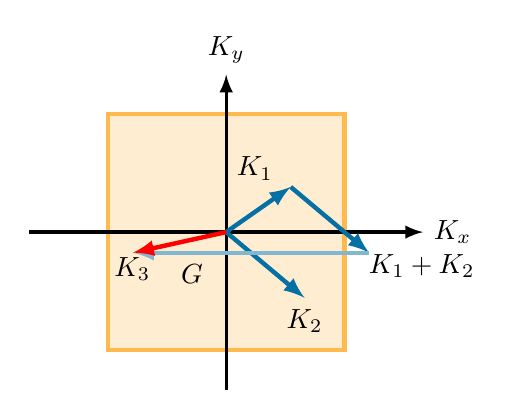
\begin{tikzpicture}
            \draw[complementary, ultra thick, fill=complementary!25] (-1.5, -1.5) rectangle (1.5, 1.5);
            \draw[very thick, ->] (-2.5, 0) -- (2.5, 0) node[right] {\(K_x\)};
            \draw[very thick, ->] (0, -2) -- (0, 2) node[above] {\(K_y\)};
            \draw[ultra thick, highlight, ->] (0, 0) -- (35:1) node[above left, black, pos=0.9] {\(\vv{K_1}\)};
            \draw[ultra thick, highlight, ->] (0, 0) -- (-40:1.3) node[below, black] {\(\vv{K_2}\)};
            \draw[ultra thick, highlight, ->] (35:1) -- ++ (-40:1.3) node[below right, black, pos=0.85] {\(\vv{K_1} + \vv{K_2}\)};
            \draw[ultra thick, highlight!50, ->] (35:1) ++ (-40:1.3) -- ++ (-3, 0) node[below, pos=0.75, black] {\(\vv{G}\)} coordinate (K3);
            \draw[ultra thick, red, ->] (0, 0) -- (K3) node[below left, black, pos=0.69] {\(\vv{K_3}\)};
        \end{tikzpicture}
        \caption[Umklapp scattering.]{Umklapp scattering. The sum of the wave vectors, \(\vv{K_1} + \vv{K_2}\), is outside of the Brillouin zone and so the resulting phonon has its wave vector shifted by \(\vv{G}\) so that it falls in the Brillouin zone. In the process the direction of the wave vectors is reversed from pointing in the positive \(K_x\) direction to the negative \(K_x\) direction.}
        \label{fig:umklapp scattering}
    \end{figure}
    
    \subsection{Temperature Dependence}
    The phonon thermal conductivity depends on temperature in a fairly complex way.
    Broadly we split into three regions which are each dominated by a different behaviour.
    
    At high temperatures, \(T > \vartheta_{\debye}\), which corresponds to \(\boltzmann  T > \hbar\omega_{\debye}\), all phonon modes are excited, including those with large values of \(K\).
    The umklapp phonon scattering process is the most important.
    The number of photons is proportional to the temperature, and the mean free path is inversely proportional to the number of phonons, so
    \begin{equation}
        \kappa \propto \ell \propto \frac{1}{n} \propto \frac{1}{T}.
    \end{equation}
    So the thermal conductivity increases with decreasing temperature.
    
    At low temperatures, where \(T \lesssim \vartheta_{\debye}\), there is a smaller fraction of high energy phonons, where we define \enquote{high energy} to mean \(\hbar\omega > \boltzmann \vartheta_{\debye}/2\), which is approximately the average energy required in a scattering event for the resulting sum of wave vectors to be outside the Brillouin zone.
    This means that umklapp scattering is less likely.
    The number of suitable phonons decreases as the Boltzmann factor
    \begin{equation}
        \exp\left[ -\frac{\frac{1}{2}\boltzmann \vartheta_{\debye}}{\boltzmann  T} \right].
    \end{equation}
    Hence
    \begin{equation}
        \kappa \propto \e^{\vartheta_{\debye}/(2T)}
    \end{equation}
    and so thermal conductivity increases with decreasing temperature.
    
    In the very low temperature regime, \(T \ll \vartheta_{\debye}\), the mean free path is approximately given be the distance between crystal defects, since phonon-phonon scattering becomes minimal.
    This value is constant and so
    \begin{equation}
        \kappa = \frac{1}{3}Cv\ell \propto T^3
    \end{equation}
    since \(C\propto T^3\), and \(v\) and \(\ell\) are approximately constant.
    The thermal conductivity then decreases with decreasing temperature.
    
    \chapter{Free Electron Gas}
    To exactly model a solid we would need to contend with approximately \(10^{23}\) atoms per centimetre cubed.
    All nuclei and electrons interact with all other nuclei and electrons via both electromagnetic effects and quantum effects, such as the Pauli exclusion principle.
    Clearly this is completely intractable and we need drastic simplifications to be able to get a workable model.
    
    One set of approximations is the \defineindex{Born--Oppenheimer approximation}, also known as the \define{adiabatic approximation}\index{adiabatic approximation|see{Born--Oppen\-heimer approximation}}.
    In this we decouple the motion of ionic cores and electrons, essentially assuming that the heavy, relatively slow moving, ionic cores are stationary, and simply act to keep the electrons inside the material.
    
    This is useful since many properties relate mostly to electronic \emph{or} atomic motion, allowing us to ignore one component of the model.
    For example, the phonon vibrations of the previous section where a result of vibrations of the atomic cores.
    This allowed us to derive many properties, such as the lattice heat capacity and thermal conductivity.
    Electrons also contribute to this, but in a way that is independent of the lattice, and we can quantify this in the Born--Oppenheimer approximation.
    
    The approximation that we make is that the valence electrons are free to move with relatively few interactions with the ionic cores, and hence we can treat the free electrons as an electron gas.
    Attempts to do so with classical statistics failed to make accurate predictions.
    We need to account for the fermionic nature of electrons, in particular for the Pauli exclusion principle.
    
    The assumptions of the free electron Fermi gas model are
    \begin{itemize}
        \item We can treat electrons as a gas of particles subject to the Pauli exclusion principle.
        \item Between collisions electrons don't interact with other electrons, called the \defineindex{independent electron approximation}.
        \item Electrons don't interact with the ions, instead the ions simply restrict the electrons motion by providing an approximately square well, called the \defineindex{free electron approximation}.
        \item Collisions are instantaneous.
        \item Electrons are in thermal equilibrium with their surroundings.
    \end{itemize}
    Notice that these are essentially the assumptions of the ideal gas, but with the added requirement of Pauli exclusion principle, and two species, electrons and ions, instead of just one.
    
    \section{Electrons in a Box}
    \subsection{One Dimension}
    \begin{figure}
        \tikzsetnextfilename{ionic-potentials-approx-square-well}
        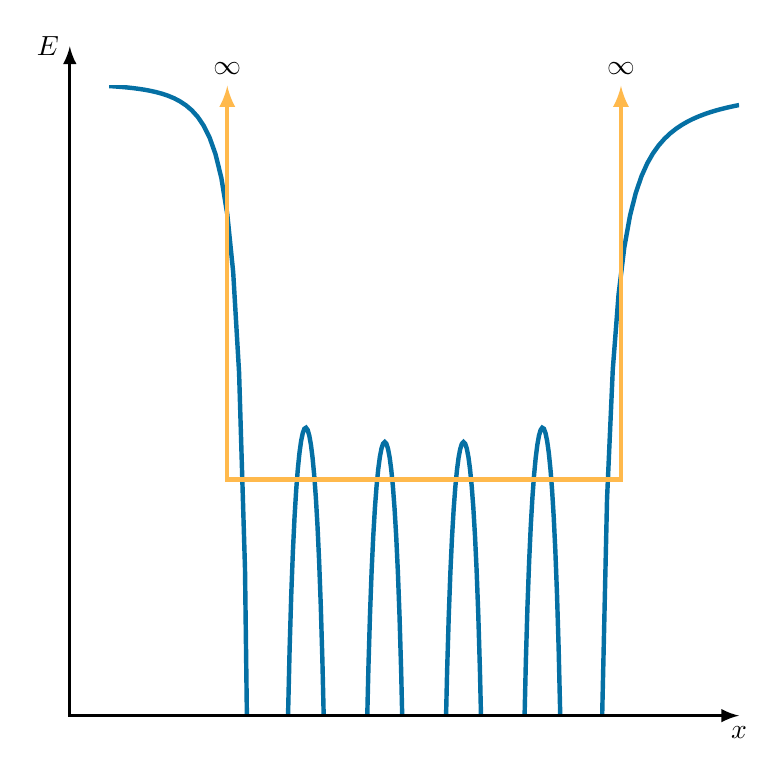
\begin{tikzpicture}[
            declare function = {potential(\x) = -0.5*(1/\x^2 + 1/(\x - 1)^2 + 1/(\x - 2)^2 + 1/(\x - 3)^2 + 1/(\x - 4)^2);}
            ]
            \begin{scope}[plot line/.style={highlight, ultra thick}]
                \clip (-2, -8) rectangle (6, 0);
                \draw[domain=-2:-0.2, plot line] plot (\x, {-potential(\x)});
                \draw[domain=0.25:0.75, plot line] plot (\x, {potential(\x)});
                \draw[domain=1.25:1.75, plot line] plot (\x, {potential(\x)});
                \draw[domain=2.25:2.75, plot line] plot (\x, {potential(\x)});
                \draw[domain=3.25:3.75, plot line] plot (\x, {potential(\x)});
                \draw[domain=4.25:6, plot line] plot (\x, {potential(\x)});
            \end{scope}
            \draw[ultra thick, complementary, <->] (-0.5, 0) node[black, above] {\(\infty\)} -- ++ (0, -5) -- ++ (5, 0) -- ++ (0, 5) node[black, above] {\(\infty\)};
            \draw[very thick, <->] (-2.5, 0.5) node[left] {\(E\)} -- (-2.5, -8) -- (6, -8) node[below] {\(x\)};
        \end{tikzpicture}
        \caption[Ionic potentials approximate an infinite square well]{The periodic ionic potential in a material can be approximated as an infinite square well potential, where the potential is finite only inside the material.}
        \label{fig:ionic potential square well}
    \end{figure}
    
    In one dimension we can treat the electrons as being in an infinite square well, of width \(L\), produced by the net ionic potential, see \cref{fig:ionic potential square well}.
    The independent electron approximation allows us to consider a single electron.
    The electron's wave function, \(\psi_n\), must satisfy the Schr\"odinger equation for a free particle inside the box:
    \begin{equation}
        \operator{\hamiltonian}\psi_n(x) = -\frac{\hbar^2}{2m} \diff[2]{\psi_n}{x} = \varepsilon_n\psi_n(x).
    \end{equation}
    The boundary conditions being that \(\psi_n\) vanishes at \(0\) and \(L\).
    
    The solutions are
    \begin{equation}
        \psi_n(x) = A\sin\left( \frac{2\pi}{\lambda_n} \right), \qqwhere \lambda_n = \frac{2 L}{n}
    \end{equation}
    with \(n \in \integers\), and
    \begin{equation}
        \varepsilon_n = \frac{\hbar^2}{2m} \left( \frac{n\pi}{L} \right)^2.
    \end{equation}
    Each energy level can be occupied by two electrons, one with spin up and the other with spin down.
    
    \subsection{Three Dimensions}
    In three dimensions the same analysis holds, we now consider a three-dimensional infinite square well, which is simply a cube in space which the electrons are constrained to be in.
    The single electron wave function, \(\psi_{\vv{k}}\), must satisfy the three-dimensional Schr\"odinger equation for a free particle inside this box:
    \begin{equation}
        \hamiltonian\psi_{\vv{k}}(\vv{r}) = -\frac{\hbar^2}{2m}\laplacian \psi_{\vv{k}}(\vv{r}) = -\frac{\hbar^2}{2m} \left[ \diff[2]{}{x} + \diff[2]{}{y} + \diff[2]{}{z} \right]\psi_{\vv{k}}(\vv{r}) = \varepsilon_{\vv{k}}\psi_{\vv{k}}(\vv{r}).
    \end{equation}
    
    We could use the standard boundary conditions where \(\psi_{\vv{k}}\) vanishes on the border of the box, this gives standing wave solutions as in the one-dimensional case.
    It turns out that it is more useful to use a set of boundary conditions called the \define{Born-von Karman boundary conditions}\index{Born-von Karman boundary condition}.
    These are a set of periodic boundary conditions in which
    \begin{equation}
        \psi(\vv{r} + L\ve{i}) = \psi(\vv{r})
    \end{equation}
    where \(\ve{i}\) are unit vectors parallel to the sides of the boxes.
    We can think of the wave function leaving the box and returning on the opposite side.
    This gives the box the topology of a 3-torus.
    This has the advantage of removing the surface of the crystal while keeping the crystal finite.
    
    The solutions are travelling waves, which are just normalised plane waves:
    \begin{equation}
        \psi_{\vv{k}}(\vv{r}) = \frac{1}{\sqrt{V}} \e^{i\vv{k} \cdot \vv{r}}
    \end{equation}
    where \(V = L^3\) is the volume of the box.
    The energy eigenvalues are 
    \begin{equation}
        \varepsilon_{\vv{k}} = \frac{\hbar^2}{2m}\vv{k}^2 = \frac{\hbar^2}{2m}(k_x^2 + k_y^2 + k_z^2).
    \end{equation}
    The wave vector is discretised so that
    \begin{equation}
        k_i = n_i\frac{2\pi}{L}
    \end{equation}
    for \(n_i \in \integers\).
    
    Confusingly we often refer to the states \(\psi_{\vv{k}}\) as orbitals, although they are not the same as atomic orbitals.
    These states have discrete energies, \(\varepsilon_{\vv{k}}\), which depend on the wave vector, \(\vv{k}\), which is also discrete.
    Recall that the momentum operator is defined as \(\vecoperator{p} = -i\hbar\grad\), and so the momentum is found from the eigenvalue equation
    \begin{equation}
        \vecoperator{p}\psi_{\vv{k}}(\vv{r}) = -i\hbar\grad\psi_{\vv{k}}(\vv{r}) = -\frac{i\hbar}{\sqrt{V}}\grad\e^{i\vv{k}\cdot\vv{r}} = -\frac{i\hbar}{\sqrt{V}}(-i\vv{k})\e^{i\vv{k}\cdot\vv{r}} = \hbar\vv{k}\psi_{\vv{k}}.
    \end{equation}
    Hence, we find that the momentum is
    \begin{equation}
        \vv{p} = \hbar\vv{k}.
    \end{equation}
    We can then define the velocity, by assuming that this momentum is the same as the classical momentum, and so \(\vv{v} = \vv{p}/m = \hbar\vv{k}/m\).
    The wavelength of the electron is given by de Broglie's wavelength formula:
    \begin{equation}
        \lambda = \frac{h}{p} = \frac{2\pi\hbar}{p} = \frac{2\pi}{k}
    \end{equation}
    
    \section{Fermi Surface}
    For a system of \(N\) electrons we can populate the allowed energy eigenstates in the order of increasing energy to get the ground state.
    We can put two electrons in each state, spin up and down, so the first \(N/2\) states are occupied.
    We define the \define{Fermi energy}\index{Fermi!energy}, \(\varepsilon_{\fermi}\), as the energy of the highest occupied single electron state in the ground state of the crystal, which is the highest occupied state at \qty{0}{\kelvin}.
    We define the corresponding wave vector to be the \define{Fermi wave vector}\index{Fermi!wave vector}, \(k_{\fermi}\).
    All occupied states then have energy \(E \le \varepsilon_{\fermi}\) and wave vectors with \(\abs{\vv{k}} \le k_{\fermi}\).
    
    The Fermi wave vector defines a surface in \(\vv{k}\)-space, which separates occupied and unoccupied states.
    We call this the \define{Fermi sphere}\index{Fermi!sphere}, although we will see later that it is not always a sphere.
    
    Recall that in reciprocal space every state has an attached volume \((2\pi/L)^3 = 8\pi^3/V\).
    This comes from assuming a regular grid of points and working out the volume per point.
    At \(T = \qty{0}{\kelvin}\) there is no thermal excitation.
    Filling the states starting from \(k = 0\) up to \(k = k_{\fermi}\) we have \(N\) electrons.
    The volume of the Fermi sphere, which is \(4\pi k_{\fermi}^2/3\), must be multiplied by the states per unit volume to give the total number of occupied states, there is also a factor of two since each volume can contain two states.
    This gives
    \begin{equation}
        \frac{4}{3}\pi k_{\fermi}^2 \cdot \left( \frac{8\pi^3}{V} \right)^{-1} \cdot 2 = N.
    \end{equation}
    Rearranging this we have
    \begin{equation}
        k_{\fermi} = \left( 3\pi^2\frac{N}{V} \right)^{1/3}.
    \end{equation}
    This is a useful expression as it depends on a single material parameter, \(n = N/V\), the electron number density.
    We can work this out for a single unit cell using the number of free electrons per unit cell and volume of the unit cell.
    
    From this expression we can define several other quantities, first we see that the Fermi energy can be expressed as
    \begin{equation}
        \varepsilon_{\fermi} = \frac{\hbar^2}{2m}k_{\fermi}^2 = \frac{\hbar^2}{2m} \left( 3\pi^2 \frac{N}{V} \right)^{2/3}.
    \end{equation}
    We can define the \define{Fermi temperature}\index{Fermi!temperature}, \(T_{\fermi}\) as
    \begin{equation}
        \varepsilon_{\fermi} = \boltzmann T_{\fermi},
    \end{equation}
    and the \define{Fermi velocity}\index{Fermi!velocity} as
    \begin{equation}
        v_{\fermi} = \frac{\hbar k_{\fermi}}{m} = \frac{\hbar}{m}\left( 3\pi^2\frac{N}{V} \right)^{1/3}.
    \end{equation}
    
    \begin{exm}{}{}
        Under standard conditions sodium has a BCC crystal structure with lattice parameter \(a = \qty{4.3}{\angstrom}\) for the conventional unit cell.
        It is monovalent.
        Compute the Fermi wave vector, Fermi energy, Fermi temperature, and Fermi velocity.
        The following may be useful
        \begin{equation}
            \hbar = \qty{6.58}{\electronvolt\second}, \quad \boltzmann = \qty{8.62e-5}{\electronvolt\per\kelvin}, \quad\text{and}\quad m_{\Pelectronneutral} = \qty{511}{\kilo\electronvolt\per\speedoflight\squared}.
        \end{equation}
        
        The number of electrons per unit cell is 2, since BCC has two atoms per conventional unit cell and they are monovalent so give one electron each.
        The volume of the unit cell is \(a^3 = (\qty{4.3}{\angstrom})^3\).
        Combining this
        \begin{equation}
            n = \frac{N}{V} = \frac{2}{a^3} = \frac{2}{(\qty{4.3}{\angstrom})^3} = \frac{2}{(\qty{4.3e-8}{\centi\metre})^3} = \qty{2.5e22}{\per\centi\metre\cubed}.
        \end{equation}
        The Fermi wave vector is then
        \begin{equation}
            k_{\fermi} = (3\pi^2 n)^{1/3} = (3\pi^2\cdot \qty{2.5e22}{\per\centi\metre\cubed})^{1/3} = \qty{9.1e6}{\per\centi\metre} = \qty{9.1}{\per\nano\metre}.
        \end{equation}
        The Fermi energy is
        \begin{multline}
            \varepsilon_{\fermi} = \frac{\hbar^2k_{\fermi}^2}{2m_{\Pelectronneutral}} = \frac{(\qty{6.58e-16}{\electronvolt\second})^2(\qty{9.1e9}{\per\metre})^2}{2(\qty{511000}{\electronvolt\per\speedoflight\squared})}\\ 
            = \qty{3.51e-17}{\electronvolt\speedoflight\squared\second\squared\per\meter\squared} = \qty{3.1}{\electronvolt}.
        \end{multline}
        The Fermi temperature is then
        \begin{equation}
            T_{\fermi} = \frac{\varepsilon_{\fermi}}{\boltzmann} = \frac{\qty{3.1}{\electronvolt}}{\qty{8.62e-5}{\electronvolt\per\kelvin}} = \qty{36320}{\kelvin}.
        \end{equation}
        The Fermi velocity is
        \begin{multline}
            v_{\fermi} = \frac{\hbar k_{\fermi}}{m_{\Pelectronneutral}} = \frac{(\qty{6.58e-16}{\electronvolt\second})(\qty{9.1e9}{\per\metre})}{\qty{511000}{\electronvolt\per\speedoflight\squared}}\\
            = \qty{1.17e-11}{\second\per\metre\per\speedoflight\squared} = \qty{1.05e6}{\metre\per\second} = \qty{0.0035}{\speedoflight}.
        \end{multline}
    \end{exm}
    
    Notice how high the Fermi energy is, a classical ideal gas would need to have a temperature of \(T_{\fermi} \approx \qty{36000}{\kelvin}\) to reach these kinetic energies.
    This is a consequence of Pauli's exclusion principle, which pushes up the energy of electrons just by not allowing them to fall down into already occupied states.
    All of this occurs even at \qty{0}{\kelvin}, this should make it clear why the classical gas model cannot accurately describe metals.
    
    \section{Finite Temperatures}
    \begin{rmk}
        For more details on the Fermi--Dirac distribution see the statistical mechanics part of the thermal physics course.
    \end{rmk}
    In order to describe the population of states at nonzero temperatures we need to introduce the \defineindex{Fermi--Dirac distribution}, which is the probability density function describing the distribution occupied states as a function of the energy of the state, \(\varepsilon\), the temperature, \(T\), and the \defineindex{chemical potential}, \(\mu\), which is the change in free energy when electrons are added to, or removed from, the system.
    The Fermi--Dirac distribution is given by
    \begin{equation}
        f(\varepsilon, \mu, T) = f(\varepsilon) = \frac{1}{\e^{(\varepsilon - \mu)\beta} + 1}
    \end{equation}
    where \(\beta = 1/(\boltzmann T)\).
    
    From this we can see that \(\varphi(\varepsilon = \mu) = 1/2\), which can be taken as the definition of \(\mu\).
    In general \(\mu\) is temperature dependent.
    In the limit of \(T \to 0\) we have \(\mu \to \varepsilon_{\fermi}\), since we recover the \qty{0}{\kelvin} model from before, which is just a step function that is \(1\) for \(\varepsilon < \varepsilon_{\fermi}\) and \(0\) for \(\varepsilon > \varepsilon_{\fermi}\).
    At \enquote{normal} temperatures, which is to say \(T < T_{\fermi}\) (not that difficult, \(T_{\fermi}\) tends to be fairly high), we can usually approximate \(\mu = \varepsilon_{\fermi}\) for metals.
    
    \begin{wrn}
        The chemical potential, \(\mu\), is sometimes called the \define{Fermi level}\index{Fermi!level}, do not confuse this with the Fermi energy, although both are energies with similar names.
    \end{wrn}
    
    \subsection{Density of States}
    Once again we make use the density of states, \(D(\varepsilon) = \diff{N}/{\varepsilon}\).
    For a three dimensional free electron Fermi gas if \(N(\varepsilon)\) is the total number of states with energy not exceeding \(\varepsilon\) then \(N(\varepsilon_{\fermi} = N)\) is the total number of electrons.
    We know
    \begin{equation}
        \varepsilon_{\fermi} = \frac{\hbar^2}{2m}k_{\fermi}^2 = \frac{\hbar^2}{2m}(3\pi^2\frac{N}{V})^{2/3}.
    \end{equation}
    This formula was simply derived by accounting for the volume associated with each state, and so the same applies to any energy, \(\varepsilon\), if we replace \(N\) with \(N(\varepsilon)\).
    \begin{equation}
        \varepsilon = \frac{\hbar^2}{2m}\left( 3\pi^2\frac{N(\varepsilon)}{V} \right)^{2/3}.
    \end{equation}
    Rearranging this we have
    \begin{equation}
        N(\varepsilon) = \frac{V}{3\pi^2} \left( \frac{2m}{\hbar^2} \right)^{3/2} \varepsilon^{3/2}.
    \end{equation}
    Therefore
    \begin{equation}
        D(\varepsilon) = \diff{N}{\varepsilon} = \frac{V}{2\pi^2} \left( \frac{2m}{\hbar^2} \right)^{3/2} \sqrt{\varepsilon}.
    \end{equation}
    
    A useful property therefore, that holds for a free electron gas, not in general, is that
    \begin{equation}
        D(\varepsilon) = \frac{3}{2}\frac{N(\varepsilon)}{\varepsilon}.
    \end{equation}
    
    The one further modification that we have to make when using the density of states is that we only want to integrate over the populated states.
    This means we need to include a factor of \(f(\varepsilon, \mu, T)\) in our integrals.
    For example the number of populated states is
    \begin{equation}
        N = \int_{0}^{\infty} D(\varepsilon) f(\varepsilon, \mu, T) \dd{\varepsilon}.
    \end{equation}
    We can use this to determine \(\mu\) as a function of \(T\) by computing the integral and rearranging.
    We can also compute the total energy stored in the electrons:
    \begin{equation}
        U_{\mathrm{el}} = \int_{0}^{\infty} D(\varepsilon)f(\varepsilon, \mu, T) \varepsilon \dd{\varepsilon}.
    \end{equation}
    
    \section{Electronic Heat Capacity}
    We saw in \cref{sec:debye model} that the phonon contribution to the low temperature heat capacity is proportional to \(T^3\).
    In measurements we find that the low temperature heat capacity of metals is modelled by
    \begin{equation}
        C(T) = \gamma T + AT^3,
    \end{equation}
    where the cubic term is as predicted by Debye's law:
    \begin{equation}
        C_{\mathrm{phonon}} = \frac{12\pi^4}{5}N\boltzmann \left( \frac{T}{\vartheta_{\debye}} \right)^{3}.
    \end{equation}
    The linear term must be due to the free electrons in the metal.
    We will aim to derive the value of \(\gamma\), which is called the \defineindex{Sommerfeld constant}, in this section.
    
    \subsection{Estimate}
    For a classical gas the heat capacity per particle is
    \begin{equation}
        C = \frac{3}{2}\boltzmann.
    \end{equation}
    In experiments we measure that the electronic contribution is linear, that is \(C_{\mathrm{el} \propto T}\).
    At room temperature we find that
    \begin{equation}
        C_{\mathrm{el}} \approx 0.001 \cdot \frac{3}{2}\boltzmann
    \end{equation}
    per electron.
    
    For a free electron gas only electrons close to the Fermi energy, \(\varepsilon_{\fermi}\), can be thermally excited.
    The faction of electrons that we consider to be \enquote{close} is \(T/T_{\fermi}\).
    The kinetic energy of an electron in the free electron gas is
    \begin{equation}
        U = \frac{3}{2}\boltzmann T.
    \end{equation}
    Therefore if there are \(N\) electrons and the fraction that can be excited is \(T/T_{\fermi}\) the kinetic energy of all electrons is
    \begin{equation}
        U_{\mathrm{el}} \approx \frac{3}{2}N\boltzmann T \frac{T}{T_{\fermi}} = \frac{3}{2}\boltzmann \frac{T^2}{T_{\fermi}}.
    \end{equation}
    
    We then approximate the electronic heat capacity as
    \begin{equation}\label{eqn:electronic heat capacity estimate}
        C_{\mathrm{el}} = \diff{U_{\mathrm{el}}}{T} \approx 3N\boltzmann \frac{T}{T_{\fermi}}.
    \end{equation}
    We see that \(C_{\mathrm{el}}\) is lower than the classical value, \(3N\boltzmann T\), by a fraction of \(T/T_{\fermi} \approx 0.01\), so this agrees reasonably well with experimental results.
    
    \subsection{Electronic Heat Capacity}
    Consider a free electron gas of \(N\) electrons.
    We assume that we are working at \enquote{normal} temperatures, by which we mean \(T \ll T_{\fermi}\), which means \(\boltzmann T \ll \varepsilon_{\fermi}\), and \(\mu \approx \varepsilon_{\fermi}\).
    The electronic heat capacity is defined as
    \begin{equation}
        C_{\mathrm{el}} \coloneqq \diff{U_{\mathrm{el}}}{T}
    \end{equation}
    where \(U_{\mathrm{el}}\) is the energy of the electrons.
    Since the electrons are free in our model the only change in energy can come from changing kinetic energy, which come from thermal excitations.
    
    In order to evaluate the derivative,
    \begin{equation}
        \diff{U_{\mathrm{el}}}{T}
    \end{equation}
    we insert a constant, \(U_{\mathrm{el}}(0)\), and define
    \begin{equation}
        \Delta U \coloneqq U_{\mathrm{el}}(T) - U_{\mathrm{el}}(0).
    \end{equation}
    We then have
    \begin{equation}
        \diff{}{T}\Delta U = \diff{}{T}U_{\mathrm{el}}(T) - \diff{}{T}U_{\mathrm{el}}(0) = \diff{}{T}U_{\mathrm{el}}(T).
    \end{equation}
    
    \begin{figure}
        \tikzsetnextfilename{increase-electron-ke-in-steps}
        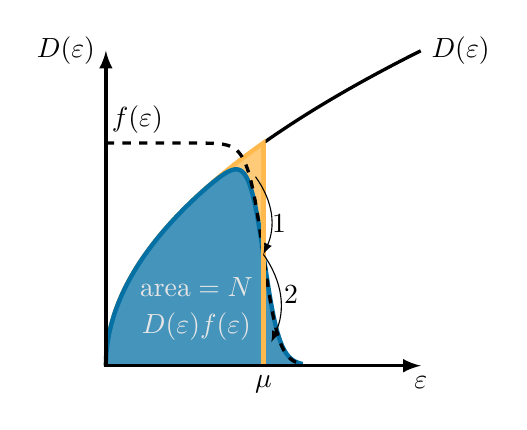
\begin{tikzpicture}
            \draw[domain=0:4, very thick, samples=1000] plot (\x, {2*sqrt(\x)})  node[right] {\(D(\varepsilon)\)};
            \draw[domain=0:2, complementary, fill=complementary!75, ultra thick, samples=1000] plot (\x, {2*sqrt(\x)}) -- (2, 0);
            \draw[domain=0:2.5, highlight, fill=highlight!75, ultra thick, samples=1000] plot (\x, {2*sqrt(\x) / (exp(10*(\x-2)) + 1)});
            \draw[domain=0:2.5, very thick, dashed, samples=1000] plot (\x, {2*sqrt(2)/(exp(10*(\x-2)) + 1)});
            \node[above] at (0.4, {2*sqrt(2)}) {\(f(\varepsilon)\)};
            \draw[complementary, ultra thick] (2, {2*sqrt(2)}) -- (2, 0);
            \draw[very thick, <->] (0, 4) node[left] {\(D(\varepsilon)\)} -- (0, 0) -- (4, 0) node[below] {\(\varepsilon\)};
            
            \node[white!90!black] at (1.15, 1) {\(\mathrm{area} = N\)};
            \node[white!90!black] at (1.15, 0.5) {\(D(\varepsilon)f(\varepsilon)\)};
            \draw[->] (1.9, 2.4) to[bend left] (2, {sqrt(2)});
            \draw[->] (2, {sqrt(2)}) to[bend left] (2.1, 0.3);
            \node at (2.2, 1.8) {1};
            \node at (2.35, 0.9) {2};
            \node[below] at (2, 0) {\(\mu\)};
        \end{tikzpicture}
        \caption{In blue is \(D(\varepsilon)f(\varepsilon)\) at \(T > 0\), in yellow is \(D(\varepsilon)f(\varepsilon)\) at \(T = 0\), the black line is \(D(\varepsilon)\), and the dashed line is \(f(\varepsilon)\). When increasing the temperature from \(0\) to some finite temperature we can do so in two steps, first taking all electrons that will become excited to energy \(\varepsilon_{\fermi}\), and then to their final, higher energy.}
        \label{fig:stepping electron energies}
    \end{figure}
    
    We can consider what happens to the energy by considering two steps.
    First we excite electrons to energy \(\varepsilon_{\fermi}\), and then to their final energy, note that this is purely theoretical, the exclusion principal forbids exciting all the electrons to the same state at once.
    See \cref{fig:stepping electron energies}.
    We therefore increase the kinetic energy in two steps.
    For the first step the energy change is
    \begin{equation}
        \Delta U_1 = \int_{0}^{\varepsilon_{\fermi}} [\varepsilon_{\fermi} - \varepsilon][1 - f(\varepsilon)]D(\varepsilon) \dd{\varepsilon},
    \end{equation}
    where \(\varepsilon\) is their initial energy and so \(\varepsilon_{\fermi} - \varepsilon\) is the energy needed to excite them to the Fermi energy.
    We use the distribution \(1 - f(\varepsilon)\), since we need to count the states that are no longer occupied after thermal excitation.
    
    For the second step the energy change is
    \begin{equation}
        \Delta U_2 = \int_{\varepsilon_{\fermi}}^{\infty} [\varepsilon - \varepsilon_{\fermi}]f(\varepsilon)D(\varepsilon) \dd{\varepsilon}
    \end{equation}
    where \(\varepsilon\) is the final energy, and so \(\varepsilon - \varepsilon_{\fermi}\) is the increase needed to reach their excited energies from the Fermi energy.
    
    Hence
    \begin{align}
        \Delta U &= \Delta U_1 + \Delta U_2\\
        &= \int_{0}^{\varepsilon_{\fermi}} [\varepsilon_{\fermi} - \varepsilon][1 - f(\varepsilon)]D(\varepsilon) \dd{\varepsilon} + \int_{\varepsilon_{\fermi}}^{\infty} [\varepsilon - \varepsilon_{\fermi}]f(\varepsilon)D(\varepsilon) \dd{\varepsilon}\\
        &= \int_{0}^{\varepsilon_{\fermi}} [\varepsilon_{\fermi} - \varepsilon]D(\varepsilon) \dd{\varepsilon} + \int_{0}^{\varepsilon_{\fermi}} [\varepsilon_{\fermi} - \varepsilon] f(\varepsilon)D(\varepsilon) \dd{\varepsilon}\\
        &\qquad\qquad+ \int_{\varepsilon_{\fermi}}^{\infty} [\varepsilon - \varepsilon_{\fermi}]f(\varepsilon)D(\varepsilon) \dd{\varepsilon}\\
        &= \int_{0}^{\infty} [\varepsilon - \varepsilon_{\fermi}] f(\varepsilon)D(\varepsilon) \dd{\varepsilon} + \text{constant}.
    \end{align}
    The constant here being the first integral, which is constant with respect to temperature, since \(f(\varepsilon)\) doesn't appear in the first integral, and this is the only temperature dependent part.
    
    We then have
    \begin{align}
        C_{\mathrm{el}} &= \diff{U_{\mathrm{el}}}{T}\\
        &= \diff{}{T}\Delta U\\
        &= \diff{}{T} \int_{0}^{\infty} [\varepsilon - \varepsilon_{\fermi}]f(\varepsilon)D(\varepsilon) \dd{\varepsilon}\\
        &= \int_{0}^{\infty} [\varepsilon - \varepsilon_{\fermi}] \diff{f}{T} D(\varepsilon)\dd{\varepsilon}
    \end{align}

    In order to evaluate this we need to consider \(f\).
    The Fermi--Dirac distribution is approximately constant at low and high temperatures, and is steeply decreasing in a region of width \(2\boltzmann T\) about \(\varepsilon_{\fermi}\).
    Assuming that \(D(\varepsilon)\) varies slowly around\(\varepsilon_{\fermi} \pm \boltzmann T\) we can treat \(\diff{f}/{T}\) a bit like a delta distribution and we have
    \begin{equation}
        C_{\mathrm{el}} = \int_{0}^{\infty} [\varepsilon - \varepsilon_{\fermi}] \diff{f}{T} D(\varepsilon)\dd{\varepsilon} \approx D(\varepsilon_{\fermi}) \int_{0}^{\infty} [\varepsilon - \varepsilon_{\fermi}] \diff{f}{T} \dd{\varepsilon}
    \end{equation}
    where the integral now provides normalisation.
    
    This integral is now material independent.
    In order to calculate the integral we write the Fermi--Dirac distribution as
    \begin{equation}
        f(\varepsilon, \varepsilon_{\fermi}, \tau) = \frac{1}{\e^{\varepsilon - \varepsilon_{\fermi}/\tau} + 1}
    \end{equation}
    where we will later set \(\tau = \boltzmann T\) and we have used \(\mu \approx \varepsilon_{\fermi}\).
    We therefore have
    \begin{equation}
        \diff{f}{\tau} = \frac{\varepsilon - \varepsilon_{\fermi}}{\tau^2} \frac{\e^{(\varepsilon - \varepsilon_{\fermi})/\tau}}{[\e^{(\varepsilon - \varepsilon_{\fermi})/\tau} + 1]^2} = \frac{1}{\boltzmann} \diff{f}{T}.
    \end{equation}
    Now let \(x = (\varepsilon - \varepsilon_{\fermi})/\tau = (\varepsilon - \varepsilon_{\fermi})/(\boltzmann T)\), and we have
    \begin{equation}
        C_{\mathrm{el}} = \boltzmann^2 TD(\varepsilon_{\fermi}) \int_{-\varepsilon_{\fermi}\beta}^{\infty} \frac{x^2\e^{x}}{[\e^{x} + 1]}.
    \end{equation}
    For \enquote{normal} temperatures the integrand is vanishingly small outside of the region of integration, which is for \(x < -\varepsilon_{\fermi}\beta\), we can therefore extend the region of integration down to negative infinity and look up the integral:
    \begin{equation}
        \int_{-\infty}^{\infty} \frac{x^2\e^{x}}{[\e^{x} + 1]^2} \dd{x} = \frac{\pi^2}{3}.
    \end{equation}
    We then have
    \begin{equation}
        C_{\mathrm{el}} \approx \frac{1}{3}\pi^2\boltzmann^2 TD(\varepsilon_{\fermi}).
    \end{equation}

    For a three-dimensional free electron gas recall that
    \begin{equation}
        D(\varepsilon) = \frac{3}{2}\frac{N(\varepsilon)}{\varepsilon},
    \end{equation}
    and so
    \begin{equation}
        D(\varepsilon_{\fermi}) = \frac{3N}{2\varepsilon_{\fermi}} = \frac{3N}{2\boltzmann T_{\fermi}}
    \end{equation}
    where we have used \(N = N(\varepsilon_{\fermi})\).
    We therefore have
    \begin{equation}
        C_{\mathrm{el}} = \frac{1}{2}\pi^2 N\boltzmann \frac{T}{T_{\fermi}}.
    \end{equation}
    This differs from the estimate in \cref{eqn:electronic heat capacity estimate} by only a constant factor, here we have \(\pi^2/2 \approx 4.93\) instead of 3.
    This result is linear in \(T\), and also significantly lower than the classical heat capacity prediction of \(C = 3N\boltzmann /2\).
        
    \subsection{Thermal Effective Mass}
    Experimentally if we measure the heat capacity and plot \(T^2\) against \(C/T\) we get a straight line described by
    \begin{equation}
        \frac{C}{T} = \gamma + AT^2.
    \end{equation}
    So, the \(y\)-intercept gives the value of \(\gamma\).
    
    If we do this we find that the value of \(\gamma\) that we have computed,
    \begin{equation}
        \gamma_{\mathrm{FEG}} = \frac{1}{2}\pi^2N\boltzmann\frac{1}{T_{\fermi}},
    \end{equation}
    using the free electron gas model is not quite equal to the experimental value, \(\gamma_{\mathrm{exp}}\).
    Of course, this is because the free electron gas is just an approximation, although it does get quite close to the actual value for simple crystals.
    For example, for potassium, with the BCC crystal structure and lattice parameter \(a = \qty{5.23}{\angstrom}\) we find that \(N/V = 2/a^3\) and so
    \begin{equation}
        T_{\fermi} = \frac{1}{\boltzmann} \frac{\hbar^2}{2m} \left( 3\pi^2\frac{N}{V} \right)^{2/3} \approx \qty{24600}{\kelvin}.
    \end{equation}
    We then find that, for one mole (\(N = \avogadro\)) of electrons (\(m = m_{\mathrm{e}}\)), we expect
    \begin{equation}
        \gamma_{\mathrm{FEG}} = \qty{1.67}{\milli\joule\per\mole\per\kelvin\squared}
    \end{equation}
    which is close to the experimental value of
    \begin{equation}
        \gamma_{\mathrm{exp}} = \qty{2.08}{\milli\joule\per\mole\per\kelvin\squared}.
    \end{equation}
    For as many approximations as we made in the free electron gas model an error of about \qty{20}{\percent} is pretty good.
    
    The Sommerfeld parameter, \(\gamma\), is proportional to the inverse Fermi temperature, which is in turn proportional to the electron mass.
    We define a new quantity, called the \defineindex{thermal effective mass}
    \begin{equation}
        m_{\mathrm{th}} \coloneqq m_{\mathrm{e}} \frac{\gamma_{\mathrm{exp}}}{\gamma_{\mathrm{FEG}}},
    \end{equation}
    which we can think of as being the mass that an electron would have to have for our calculation to match the experimental result.
    
    Typically for simple metals we find that \(m_{\mathrm{th}}\) is between one and two times the electron mass, but for more complicated metals, such as the \(\mathrm{d}\)-block \ce{Fe}, \ce{Co}, or \ce{Ni}, the thermal mass can be more like ten or fifteen times the electron mass.
    For the so called heavy fermion metals, such as \ce{CeAl_3}, \ce{CeCu_2Si_2}, and \ce{UBe_13}, with lots of \(\mathrm{f}\) electrons, we find that the thermal mass can be 100 to \num{1000} times the electron mass.
    One explanation for why the electrons appear to be more massive is because we aren't taking into account their interaction with the crystal potential, we will do so later.
    We also aren't accounting for electron-phonon or electron-electron interactions.
    
    \section{Electrical Conductivity}
    Ohm's law states that \(I = V/R\) for current, \(I\), voltage, \(V\), and resistance, \(R\).
    A more general form of Ohm's law in terms of the current density, \(\vv{j}\), electric field, \(\vv{E}\), resistivity, \(\rho\), and electrical conductivity, \(\sigma = 1/\rho\) (assuming an isotropic medium)
    \begin{equation}
        \vv{j} = \frac{1}{\rho} \vv{E} = \sigma \vv{E}.
    \end{equation}
    Experimentally we find that for most metals at room temperature or above the resistivity is approximately linear in \(T\).
    
    For a free electron Fermi gas in an electric field we have that the force is given by
    \begin{equation}
        \vv{F} = m \diff{\vv{v}}{t} = \hbar\diff{\vv{k}}{t} = -e\vv{E}.
    \end{equation}
    If there is no scattering then we expect that
    \begin{equation}
        \delta\vv{k}(t) = \vv{k}(t) - \vv{k}(0) = -\frac{et}{\hbar}\vv{E}.
    \end{equation}
    From this we would expect that all of the electrons are accelerated with acceleration \(\hbar\,\delta\vv{k}(t)/m\), this corresponds to the Fermi sphere, and all states within, being shifted by \(\delta\vv{k}(t)\).
    This is correct for small time scales, but doesn't give a stead-state solution since the velocity becomes arbitrarily large.
    
    The reason for this non-physical behaviour is we haven't considered scattering, which slows the electrons down.
    We still assume that all electrons have the same acceleration, but now that they scatter with an average time \(\tau\) between collisions.
    Therefore we instead find that
    \begin{equation}
        \delta\vv{k} = -\frac{e\tau}{\hbar}\vv{E}.
    \end{equation}
    The average electron velocity, which is called the \defineindex{drift velocity}, is given by
    \begin{equation}
        \vv{v_{\mathrm{d}}} = \frac{\hbar}{m}\delta\vv{k} = -\frac{e\tau}{m}\vv{E}.
    \end{equation}
    The current density is then given by the drift velocity times the charge and the charge carrier density,
    \begin{equation}
        \vv{j} = -en\vv{v_{\mathrm{d}}} = \frac{ne^2\tau}{m}\vv{E} = \sigma\vv{E}.
    \end{equation}
    Hence, the electrical conductivity is
    \begin{equation}
        \sigma = \frac{ne^2\tau}{m}.
    \end{equation}
    This is called the \defineindex{Drude model}, or sometimes the Drude--Sommerfeld model.
    
    \subsection{Resistivity Temperature Dependence}
    In this model the resistivity is
    \begin{equation}
        \rho = \frac{1}{\sigma} = \frac{m}{ne^2\tau}.
    \end{equation}
    The temperature dependence here enters through the scattering time, \(\tau\), which we can relate to the scattering rate, \(\tau^{-1}\).
    At high temperatures, \(T > \vartheta_{\debye}\), the scattering rate, \(\tau^{-1}\), is proportional to the average phonon density, \(\expected{n_{\mathrm{ph}}}\).
    This in turn is proportional to \(T\) in the high temperature regime, and so \(\rho \propto \tau^{-1} \propto \expected{n_{\mathrm{ph}}} \propto T\).
    This agrees with experimental observations.
    We are assuming here that electron-phonon scattering is the dominant scattering type at high temperatures.
    
    We can be more accurate if we consider a variety of types of scattering.
    There are three types of scattering, electron-phonon scattering, with scattering time \(\tau_{\mathrm{ph}}\), as discussed above, scattering off of static crystal defects, with scattering time \(\tau_{\mathrm{defects}}\), and electron-electron scattering, with scattering time \(\tau_{\mathrm{el}}\).
    We can define the effective scattering time, \(\tau\), to satisfy
    \begin{equation}
        \frac{1}{\tau} = \frac{1}{\tau_{\mathrm{ph}}} + \frac{1}{\tau_{\mathrm{defects}}} + \frac{1}{\tau_{\mathrm{el}}}.
    \end{equation}
    
    In the very low temperature regime we see that the resistivity is approximately constant.
    In this regime both electron-electron and electron-phonon scattering rates go to zero so this must be due to scattering off of static defects.
    
    So, in order to determine the temperature dependence of the scattering rate we need to know the temperature dependence for each type of scattering.
    
    The scattering rate for scattering off of defects is approximately constant, since the number of defects doesn't change with temperature.
    This is the predominant scattering type at very low temperatures.
    
    At low to intermediate temperatures the temperature dependence is quite complicated.
    The electron-electron scattering rate is depends on the number of electrons present to scatter, and the number of electrons present to scatter off, and so is proportional to \(T^2\).
    
    The electron-phonon scattering rate is more complex.
    Suppose that an electron is scattered from a state with wave vector \(\vv{k}\) to a state with wave vector \(\vv{k'}\), due to an interaction with a phonon with wave vector \(\vv{q}\).
    Conservation of momentum means we must have
    \begin{equation}
        \vv{k'} = \vv{k} + \vv{q}.
    \end{equation}
    Conservation of energy means that we must have
    \begin{equation}
        \varepsilon' = \varepsilon \pm \hbar \omega_{\text{phonon}} \approx \varepsilon
    \end{equation}
    where \(\varepsilon\)  is the energy of the initial state, \(\varepsilon'\) is the energy of the final state, and \(\hbar\omega_{\text{phonon}}\) is the energy of the phonon, which is significantly smaller than the energy of the electrons, since phonon energies are typically a few \unit{\milli\electronvolt} whereas electron energies are a few \unit{\electronvolt}.
    We say that the scattering is quasi-elastic, since the energy change is mostly negligible.
    
    There are further constraints due to the exclusion principle.
    First, the electron must scatter from a an occupied state, but it must also be close enough to the Fermi energy that it can be scattered, hence we must have \(k \lessapprox k_{\fermi}\).
    The electron must scatter into an unoccupied state, so \(k' \gtrapprox k_{\fermi}\).
    We therefore have
    \begin{equation}
        k \approx k' \approx k_{\fermi}.
    \end{equation}
    Essentially meaning that only electrons in states near the Fermi surface can scatter, and that they scatter to states near the Fermi surface.
    
    We will see in a later section % TODO: Add link to this later section on Bloch theorem
    that electrons in a periodic potential have periodic wave functions.
    This means that for every state outside of the first Brillouin zone there is an equivalent state in the first Brillouin zone.
    For this reason we get normal and umklapp scattering, just as with phonons.
    
    In normal scattering the change in direction of travel is small.
    For multiple normal scattering events the net effect tends to cancel and therefore normal scattering has a negligible contribution to electrical resistivity, apart from at very low temperatures when there aren't many phonons with enough energy to scatter an electron into the next Brillouin zone.
    
    In umklapp scattering we can reduce \(\vv{k} + \vv{q}\) to a wave vector in the first Brillouin zone by addition of a lattice vector, \(\vv{G}\), such that \(\vv{k'} = \vv{k} + \vv{q} + \vv{G}\) is in the first Brillouin zone.
    Typically these electrons will end up in states on the opposite side of the Brillouin zone, having only just entered the neighbouring Brillouin zone.
    For this reason the direction change in these types of scattering events is large.
    Therefore there is a significant contribution to the electrical resistivity from umklapp scattering, apart from at very low temperatures when there aren't enough energetic phonons.
    
    In order for umklapp scattering to happen we need phonons with \(q > q_0\), where \(q_0\) is the difference in wave vectors between the closest points on Fermi surfaces in neighbouring Brillouin zones.
    The number of phonons that satisfy this is given by a Boltzmann factor, \(\e^{-\vartheta_{\umklapp}/T}\), where \(\vartheta_{\umklapp}\) is a characteristic material property, with dimensions of temperature.
    Therefore the electron-phonon scattering at low to intermediate temperatures is proportional to \(\e^{-\vartheta_{\umklapp}/T}\).
    
    To summarise the temperature dependence of the scattering rate:
    \begin{itemize}
        \item At very low temperatures, \(T \ll \vartheta_{\debye}\), resistivity approaches a constant value as most scattering occurs due to defects in the crystal.
        \item At low to intermediate temperatures the temperature dependence is more complex.
        In particular the contribution from electron-electron scattering scales as \(T^2\) and the contribution from electron-phonon scattering scales as \(\e^{-\vartheta_{\umklapp}/T}\).
        \item At high temperatures, \(T > \vartheta_{\debye}\), the scattering rate is proportional to \(T\), since electron-phonon scattering is dominant and there are plenty of phonons.
    \end{itemize}
    
    \section{Electronic Thermal Conductivity}
    In a metal electrons have a non-negligible contribution to the transport of heat.
    The overall thermal conductivity, \(\kappa\), is given by \(\kappa = \kappa_{\mathrm{el}} + \kappa_{\mathrm{ph}}\), where \(\kappa_{\mathrm{el}}\) and \(\kappa_{\mathrm{ph}}\) are the contributions due to electrons and phonons respectively.
    
    For metals the thermal conductivity is lowest at low temperatures, it then increases with temperature up to a point, then starts decreasing again as umklapp scattering becomes more important.
    
    We will use the same model for electronic thermal conductivity as we did for phononic thermal conductivity in \cref{sec:lattice thermal conductivity}, namely that
    \begin{equation}
        \kappa_{\mathrm{el}} = \frac{1}{3}C_{\mathrm{el}}v\ell
    \end{equation}
    where \(v\) is the particle velocity, \(\ell\) is the mean free path, and \(C_{\mathrm{el}}\) is the electronic heat capacity, which is given by
    \begin{equation}
        C_{\mathrm{el}} = \frac{1}{V} \frac{1}{2}\pi^2N\boltzmann \frac{T}{T_{\fermi}}.
    \end{equation}
    The Fermi temperature is given by
    \begin{equation}
        T_{\fermi} = \frac{\varepsilon_{\fermi}}{\boltzmann} = \frac{\frac{1}{2}mv_{\fermi}^2}{\boltzmann}.
    \end{equation}
    The mean free path is given by
    \begin{equation}
        \ell \approx v_\fermi \tau.
    \end{equation}
    We also define the electron density to be \(n = N/V\).
    
    Putting this all together we find that
    \begin{equation}
        \kappa_{\mathrm{el}} = \frac{\pi^2\boltzmann^2 n}{3m}T\tau.
    \end{equation}
    At high temperatures this is approximately linear in \(T\).
    At lower temperatures the temperature dependence becomes more complicated as we have to consider the temperature dependence of \(\tau\).
    
    It is possible to relate the thermal conductivity to the electrical conductivity, which we calculated earlier was
    \begin{equation}
        \sigma = \frac{ne^2\tau}{m}.
    \end{equation}
    To do so we compare their ratio:
    \begin{equation}
        \frac{\kappa_{\mathrm{el}}}{\sigma} = \frac{\pi^2}{3} \left( \frac{\boltzmann}{e} \right)^2 T = L_{\mathrm{FEG}} T.
    \end{equation}
    Here we define the \defineindex{Lorenz number}, \(L\), to be
    \begin{equation}
        L = \frac{\kappa_{\mathrm{el}}}{\sigma T}.
    \end{equation}
    This is approximately constant, a fact referred to as the \defineindex{Widemann--Franz law}.
    For the free electron gas model we have
    \begin{equation}
        L_{\mathrm{FEG}} = \qty{2.44e-8}{\watt\ohm\per\kelvin\squared}.
    \end{equation}
    This turns out to be quite close to experimental values, which is quite impressive for a model with so many approximations.
    
    \section{Magnetic Field Effects}
    For free electrons in an electric field, \(\vv{E}\), and magnetic field, \(\vv{B}\), we expect the force due to these fields to be given by
    \begin{equation}
        \vv{F} = m\diff{\vv{v}}{t} = \hbar \diff{\vv{k}}{t} = -e(\vv{E} + \vv{v} \times \vv{B}).
    \end{equation}

    However, we don't have free electrons, in particular we have to account for scattering.
    We do so by considering another term \(\hbar\,\delta\vv{k}/\tau\), for the same reason that we did when considering the electrical conductivity.
    The force is instead
    \begin{equation}
        \vv{F_{\mathrm{d}}} = \hbar \left( \diff{}{t} + \frac{1}{\tau} \right)\delta\vv{k} = -e(\vv{E} + \vv{v_{\mathrm{d}}} \times \vv{B}).
    \end{equation}
    Here \(\vv{F_{\mathrm{d}}}\) is the average force on an electron and \(\vv{v_{\mathrm{d}}} = \hbar\,\delta\vv{k}/m\) is the drift velocity, which is just the average velocity.
    
    Using \(m\vv{v_{\mathrm{d}}} = \hbar\delta\vv{k}\) we have
    \begin{equation}
        m\left( \diff{}{t} + \frac{1}{\tau} \right)\vv{v_{\mathrm{d}}} = -e(\vv{E} + \vv{v_{\mathrm{d}}} \times \vv{B}).
    \end{equation}
    
    We will consider only a steady-state solution, that is a solution in which the time derivative vanishes.
    The result therefore is that the entire Fermi sphere is displaced by \(\delta\vv{k}\)
    
    \subsection{Hall Effect}
    Consider a cuboidal metallic bar in an electromagnetic field, aligned such that the electric field is along the bar, which we will call the \(x\)-direction, and the magnetic field acts across the bar, which we will call the \(z\)-direction.
    The electric field, \(E_x\), generates a current density, \(j_x\), along the bar.
    This corresponds to charges moving along the \(x\)-direction.
    The Lorentz force then has a component, due to the \(\vv{v} \times \vv{B}\) term, along the \(y\)-direction, since at the instant when the magnetic field is switched on, \(\vv{v} = v_x\vh{x}\) and \(\vv{B} = B_z\vv{B}\).
    The result is that the electrons also move in the \(y\)-direction, and hence there is a slight build up of negative charge along one side and a resulting positive charge on the other side.
    We can measure this charge separation as a voltage, called the \define{Hall voltage}\index{Hall!voltage}.
    The process producing this transverse voltage is called the \define{Hall effect}\index{Hall!effect}.
    We can now work out what we expect the voltage to be for a given metal.
    
    Considering collisions in the metal the equation of motion is
    \begin{equation}
        m\left( \diff{}{t} + \frac{1}{\tau} \right)\vv{v} = -e(\vv{E} + \vv{v} \times \vv{B}),
    \end{equation}
    where we drop the subscript \(\mathrm{d}\), but are still using the drift velocity.
    The magnetic field is \(\vv{B} = (0, 0, B)\) and so we find that
    \begin{align}
        m\left( \diff{}{t} + \frac{1}{\tau} \right) v_x &= -e(E_x + Bv_y),\\
        m\left( \diff{}{t} + \frac{1}{\tau} \right) v_y &= -e(E_y - Bv_x),\\
        m\left( \diff{}{t} + \frac{1}{\tau} \right) v_x &= -eE_x.\\
    \end{align}
    For a stead-state solution the time derivative vanishes and we are left with
    \begin{align}
        v_x &= -\frac{e\tau}{m}E_x - \omega_{\mathrm{c}}\tau v_y,\\
        v_y &= -\frac{e\tau}{m}E_y + \omega_{\mathrm{c}}\tau v_x,\\
        v_z &= -\frac{e\tau}{m}E_z.
    \end{align}
    Here \(\omega_{\mathrm{c}}\) is the \defineindex{cyclotron frequency}, which is the frequency associated with the spiral an otherwise free electron follows in a magnetic field, it is given by\footnote{see the notes on the electromagnetism course for details.}
    \begin{equation}
        \omega_{\mathrm{c}} = \frac{eB}{m}.
    \end{equation}
    
    Further, in a steady-state since electrons don't leave the bar we must have that \(v_y = 0\).
    Putting this in and combining the first two equations for \(v_i\) we have
    \begin{equation}\label{eqn:Ex and Ey relation hall effect}
        E_y = \frac{m\omega_{\mathrm{c}}\tau}{e\tau}v_x = \frac{m\omega_{\mathrm{c}}}{e} \left( -\frac{e\tau}{m}E_x \right) = -\omega_{\mathrm{c}}\tau E_x = -\frac{eB\tau}{m}E_x.
    \end{equation}
    
    We can now work out the Hall voltage, \(V_{\hall}\), which is the transverse voltage measured along the \(y\)-direction.
    Over a distance \(d\) the voltage is given by \(V = Ed\).
    Using this the Hall voltage is 
    \begin{equation}
        V_{\hall} = E_yw_y,
    \end{equation}
    where \(w_y\) is the width of the bar in the \(y\)-direction.
    Let \(w_z\) be the width of the bar in the \(z\)-direction, then, using the fact that the current, \(I\), and current density, \(\vv{j}\), are related by \(j = I/A\) we can calculate the longitudinal current:
    \begin{equation}
        I_x = w_yw_z j_x.
    \end{equation}
    We define the \define{Hall coefficient}\index{Hall!coefficeint}, \(R_H\), to be
    \begin{equation}
        R_{\hall} = \frac{V_{\hall}/w_y}{I_xB/(w_yw_z)} = \frac{V_{\hall}w_z}{I_xB}.
    \end{equation}
    We can measure all of the quantities on the right fairly easily.
    We also know that
    \begin{equation}
        j_x = \sigma E_x = \frac{ne^2\tau}{m}E_x,
    \end{equation}
    for a free electron gas.
    Substituting this and \cref{eqn:Ex and Ey relation hall effect} into the definition of the Hall coefficient we have
    \begin{equation}
        R_{\hall} = \frac{E_y}{j_xB} = -\frac{eB\tau}{m}E_x \frac{m}{ne^2\tau E_x B} = -\frac{1}{ne}.
    \end{equation}
    So, since \(e\) is known, we can use the Hall coefficient as a measure of the electron density of the metal, and we can also measure the Hall coefficient just by measuring voltages, lengths, currents, and magnetic field strengths, all of which can be done fairly easily.
    
    \chapter{Electron Energy Bands}
    The free electron gas model works well for most metals.
    In order deal with the electronic properties of insulators and semiconductors we need to introduce the concept of electron energy bans, which explain some of the deviation from the free electron gas model.
    These are energy-wave vector dispersion relations for the electrons.
    We no longer treat electrons as a free electron gas, but we still assume the independent electron approximation holds.
    
    \section{Energy Bands}
    Consider a diatomic molecule.
    The bonding of such a molecule can be represented by the molecular orbital diagrams such as in \cref{fig:MO H2}.
    This gives a minimum energy for the electrons, if they are in the bonding orbital, and a maximum energy, if they are in the antibonding orbital.
    
    If we now consider many atoms of the same type then electrons involved in bonding will have more energy bands, over roughly the same range of energies.
    In the limit of a very large number of atoms the allowed energy levels become approximately continuous between the minimum and maximum values, and we call the region of allowed energies an \defineindex{energy band}.
    
    \section{Band Gaps}
    In a real metal the valence electrons aren't actually free, but move in a periodic crystal potential.
    This is given by the superposition of individual Coulomb potentials for the ionic cores, see \cref{fig:ionic potential square well}.
    The potential is typically quite weak, essentially the effect is to modify the parabolic free-electron energy dispersion, \(\varepsilon(\vv{k}) = \hbar^2k^2/(2m)\), and create band gaps, which are regions with no energy levels.
    This occurs at the Brillouin zone edges.
    The electronic properties of solids then depend on where the highest filled energy level is relative to the positions of band gaps.
    
    \begin{figure}
        \tikzsetnextfilename{band-gaps-for-different-types}
        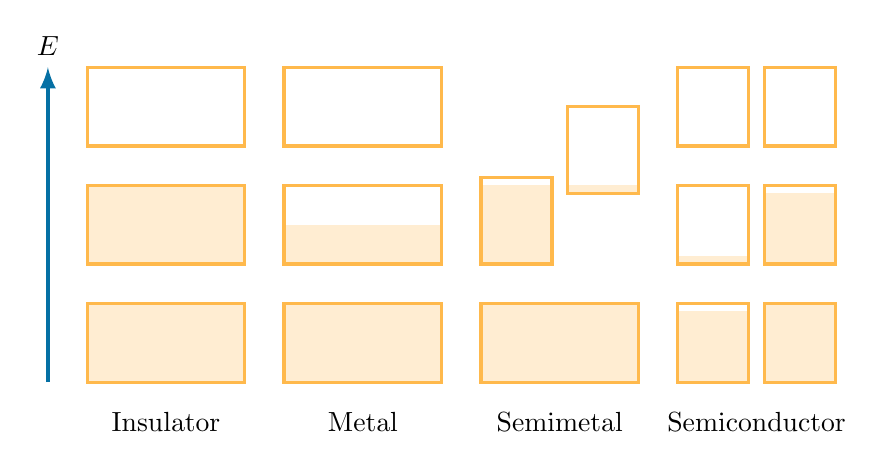
\begin{tikzpicture}
            \draw[very thick, complementary, fill=complementary!25] (0, 0) rectangle (2, 1);
            \draw[very thick, complementary, fill=complementary!25] (0, 1.5) rectangle (2, 2.5);
            \draw[very thick, complementary] (0, 3) rectangle (2, 4);
            \begin{scope}[xshift=2.5cm]
                \draw[very thick, complementary, fill=complementary!25] (0, 0) rectangle (2, 1);
                \fill[complementary!25] (0, 1.5) rectangle (2, 2);
                \draw[very thick, complementary] (0, 1.5) rectangle (2, 2.5);
                \draw[very thick, complementary] (0, 3) rectangle (2, 4);
            \end{scope}
            \begin{scope}[xshift=5cm]
                \draw[very thick, complementary, fill=complementary!25] (0, 0) rectangle (2, 1);
                \fill[complementary!25] (0, 1.5) rectangle (0.9, 2.5);
                \fill[complementary!25] (1.1, 2.4) rectangle (2, 2.5);
                \draw[very thick, complementary] (0, 1.5) rectangle (0.9, 2.6);
                \draw[very thick, complementary] (1.1, 2.4) rectangle (2, 3.5);
            \end{scope}
            \begin{scope}[xshift=7.5cm]
                \fill[complementary!25] (0, 0) rectangle (0.9, 0.9);
                \fill[complementary!25] (0, 1.5) rectangle (0.9, 1.6);
                \draw[very thick, complementary] (0, 0) rectangle (0.9, 1);
                \draw[very thick, complementary] (0, 1.5) rectangle (0.9, 2.5);
                \draw[very thick, complementary] (0, 3) rectangle (0.9, 4);
                \fill[complementary!25] (1.1, 1.5) rectangle (2, 2.4);
                \draw[very thick, complementary, fill=complementary!25] (1.1, 0) rectangle (2, 1);
                \draw[very thick, complementary] (1.1, 1.5) rectangle (2, 2.5);
                \draw[very thick, complementary] (1.1, 3) rectangle (2, 4);
            \end{scope}
            \node at (1, -0.5) {Insulator};
            \node at (3.5, -0.5) {Metal};
            \node at (6, -0.5) {Semimetal};
            \node at (8.5, -0.5) {Semiconductor};
            \draw[ultra thick, highlight, ->] (-0.5, 0) -- (-0.5, 4) node[above, black] {\(E\)};
        \end{tikzpicture}
        \caption[Band structure for different materials]{The relation between electrical behaviour relates and how full the bands are relative to the positions of band gaps.}
        \label{fig:band gaps for various types}
    \end{figure}
    
    \Cref{fig:band gaps for various types} shows approximately how band are filled for different types of materials.
    Metals have partially filled bands, which means that only a very small amount of energy is required to excite a valence electron into a slightly higher energy state, where it can be accelerated by an electric field, which results in a current.
    The size of the band gap is significantly larger than the gain in kinetic energy of a single electron due to an applied voltage, so electrons cannot be excited into the next band simply by applying a voltage.
    
    Insulators are actually very similar in band structure to metals, except that the bands are filled, and so the electrons cannot be excited by a voltage as they would have to move into the next band, and there isn't enough energy for this.
    
    Semiconductors are somewhere between, at absolute zero they behave as insulators.
    As temperature increases more and more electrons are excited thermally into the next band, which means that they become better conductors as temperature increases.
    
    Semimetals have bands that overlap, we will discuss this, and semiconductors, in the future.
    
    \section{Nearly Free Electron Model}
    To understand band splitting we start from the free electron model with plane wave states, which has no band splitting, and we introduce a periodic potential.
    The free electron wave functions are 
    \begin{equation}
        \psi_{\vv{k}}(\vv{r}) = \e^{i\vv{k}\cdot\vv{r}}.
    \end{equation}
    The energy of such a state is
    \begin{equation}
        \varepsilon_{\vv{k}} = \frac{\hbar^2}{2m}k^2 = \frac{\hbar^2}{2m}(k_x^2 + k_y^2 + k_z^2).
    \end{equation}
    The allowed values of \(k_i\) are \(2\pi n/L\) for \(n \in \naturals\) and \(L\) being the length of the crystal.
    The momentum of such a state is \(\vv{p} = \hbar\vv{k}\).
    
    Recall that the diffraction condition \(\vv{\Delta\vv{k}} = \vv{G}\), for some reciprocal lattice vector, \(\vv{G}\), or equivalently \(2\vv{k} \cdot \vv{G} = G^2\), arises when we consider plane wave electrons in exactly the same way that it arises when considering x-ray diffraction.
    Or, in one dimension, \(k = \pm G/2 = \pm n\pi/a\).
    A right-travelling electron with \(k = \pi/a\) is diffracted into a left-travelling electron with \(k = -\pi/a\), and vice versa.
    Notice that these are the same state since \(k^2\) is unchanged and both direction and wave vector are negated so \(\vv{k}\cdot\vv{r}\) is unchanged.
    
    Still in one dimension we can write our wave function as
    \begin{equation}
        \psi(\pm) = \psi_{+k}(x) \pm \psi_{-k}(x),
    \end{equation}
    which gives standing wave solutions
    \begin{equation}
        \psi(+) = 2\cos\left( \frac{\pi x}{a} \right), \qqand \psi(-) = 2i\sin\left( \frac{\pi x}{a} \right).
    \end{equation}
    The probability density is defined as \(\rho = \psi^*\psi = \abs{\psi}^2\).
    For travelling waves we have
    \begin{equation}
        \rho = \e^{ikx}\e^{-ikx} = 1.
    \end{equation}
    For the standing waves we have
    \begin{equation}
        \rho(+) = \abs{\psi(+)}^2 \propto \cos^2\left( \frac{\pi x}{a} \right), \qqand \rho(-) = \abs{\psi(-)}^2 \propto \sin^2\left( \frac{\pi x}{a} \right).
    \end{equation}
    These have maxima at \(x = na\) and \(x = (2n + 1)a/2\) respectively for \(n \in \integers\).
    This is pretty important since the ionic cores are placed at the positions \(na\) so the maxima of the \(+\) standing waves align with the ions, and the maxima of the \(-\) standing waves are directly between.
    The result is, since the potential energy scales as \(-1/r^2\), the \(+\) states are lower energy than the \(-\) states.
    We can therefore associate the \(+\) states with the lower band and the \(-\) states with the higher band.
    The bands, and the forbidden region between them, are shown in \cref{fig:energy bands one dimension}.
    
    \begin{figure}
        \tikzsetnextfilename{one-dimensional-energy-bands}
        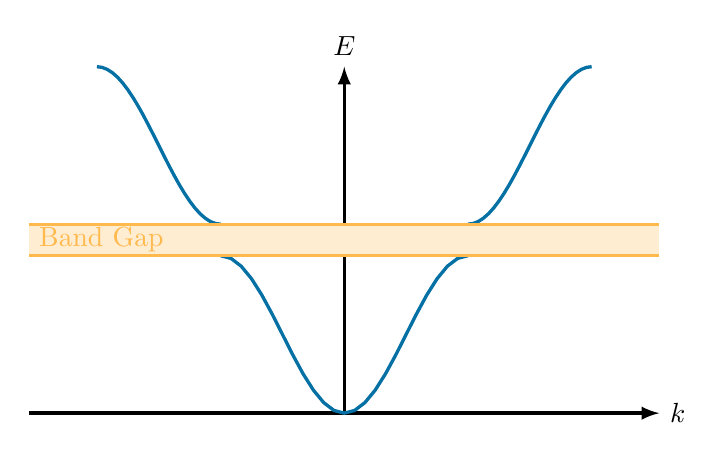
\begin{tikzpicture}
            \draw[very thick, ->] (-4, 0) -- (4, 0) node[right] {\(k\)};
            \draw[very thick, ->] (0, 0) -- (0, 4.4) node[above] {\(E\)};
            \draw[domain=-pi/2:pi/2, very thick, highlight] plot (\x, {2*sin(\x r)^2});
            \draw[domain=-pi:-pi/2, very thick, highlight] plot (\x, {2.4 + 2*cos(\x r)^2});
            \draw[domain=pi/2:pi, very thick, highlight] plot (\x, {2.4 + 2*cos(\x r)^2});
            \fill[complementary!25] (-4, 2) rectangle (4, 2.4);
            \draw[complementary, very thick] (-4, 2) -- ++ (8, 0);
            \draw[complementary, very thick] (-4, 2.4) -- ++ (8, 0);
            \node[right, complementary] at (-4, 2.2) {Band Gap};
        \end{tikzpicture}
        \caption{Energy bands separated by a band gap.}
        \label{fig:energy bands one dimension}
    \end{figure}
    
    So we know now why the splitting occurs, but not how large the splitting is.
    For this we will need to consider the potential.
    To aid our thinking we consider a simple potential with the same periodicity as the crystal potential, namely
    \begin{equation}
        U(x) = -U\cos\left( \frac{2\pi x}{a} \right).
    \end{equation}
    At the zone boundary we have the, now normalised, wave functions
    \begin{equation}
        \psi(+) = \sqrt{\frac{2}{a}} \cos\left( \frac{\pi x}{a} \right), \qqand \psi(-) = \sqrt{\frac{2}{a}} \sin\left( \frac{\pi x}{a} \right).
    \end{equation}
    The band splitting, \(E_{\gap}\), is simply the difference between the average energies of the two states, which is
    \begin{align}
        E_{\gap} &= \varepsilon_{-} - \varepsilon_{+}\\
        &= \int_{0}^{a}U(x)\abs{\psi(-)}^2 \dd{x} - \int_{0}^{a} U(x) \abs{\psi(+)}^2 \dd{x}\\
        &= \int_{0}^{a} U(x) (\abs{\psi(-)}^2 - \abs{\psi(+)}^2) \dd{x}\\
        &= -U\frac{2}{a}\int_{0}^{a} \cos\left( \frac{2\pi x}{a} \left[ \sin^2\left( \frac{\pi x}{a} \right) - \cos^2\left( \frac{\pi x}{a} \right) \right] \right) \dd{x}\\
        &= U\frac{2}{a} \int_{0}^{a} \cos^2\left( \frac{2\pi x}{a} \right) \dd{x}\\
        &= \frac{U}{a} \int_{-a}^{a} \cos^2\left( \frac{2\pi x}{a} \right) \dd{x}\\
        &= U
    \end{align}
    Here we have used the trig identity
    \begin{equation}
        \sin^2\vartheta - \cos^2\vartheta = -\cos(2\vartheta).
    \end{equation}
    We then noticed the similarity to computing Fourier components, in particular that this integral gives \(a\), since \(\cos\) is orthogonal in \(L^2([-a, a])\), and has norm \(a\).
    
    While this simple potential isn't realistic the real potential is periodic and we can always choose to have an ion at 0, and so the potential will be an even function.
    We can therefore expand it as a Fourier series.
    Doing so, and generalising to three dimensions, we find that for a realistic crystal potential, \(U\), the splitting at wave vector \(\vv{k}\) in the Brillouin zone is given by the Fourier component, \(U_{2\vv{k}}\), of the crystal potential.
    Recall that the Fourier components are only non-zero for wave vectors which coincide with reciprocal lattice vectors, hence band splittings can appear only in locations where \(2\vv{k} = \vv{G}\) for some reciprocal lattice vector \(\vv{G}\).
    In particular this requirement is met at the centre of the faces of a three-dimensional Brillouin zone, since by construction the Brillouin zone faces are halfway between reciprocal lattice points, which are separated by a reciprocal lattice vector.
    
    While the actual electronic band structure for a realistic crystal potential is too complicated to compute analytically there are several model potentials that exhibit important behaviour.
    We've already seen the cosine model, another model potential is the \defineindex{Kronig--Penny model}, which is simply a square wave.
    
    \section{Empty Lattice Approximation}
    While the ionic potential is important for a lot of materials the main splitting is due to the lattice structure.
    We therefore consider the \defineindex{empty lattice approximation}, in which we take \(U = 0\) and consider how the lattice periodicity effects the quadratic free electron dispersion relation,
    \begin{equation}
        \varepsilon_{\vv{k}} = \frac{\hbar^2}{2m}k^2.
    \end{equation}
    
    The lattice is periodic, in particular \(\varepsilon(\vv{k}) = \varepsilon(\vv{G} + \vv{k})\) for any reciprocal lattice vector \(\vv{G}\).
    There are two approaches we can take to account for this.
    One is to consider \(\varepsilon_{\vv{k}}\), and all shifts of the dispersion relation by a reciprocal lattice vector, discarding everything outside of the first Brillouin zone.
    The second is to consider \(\varepsilon_{\vv{k}}\) and map all parts outside of the Brillouin zone into the Brillouin zone by addition of an appropriate lattice vector.
    We consider both approaches in one dimension but the first is far simpler for higher dimensions.
    
    In one dimension the dispersion relation, and all \(\vv{G}\)-shifts of \(\varepsilon_{\vv{k}}\), are shown in \cref{fig:electron dispersion relation and G-shifts}.
    Restricting the result to just the Brillouin zone we get \cref{fig:restricted electron dispersion relation and all G-shifts}.
    
    \begin{figure}
        \tikzsetnextfilename{electron-dispersion-relation-and-G-shifts}
        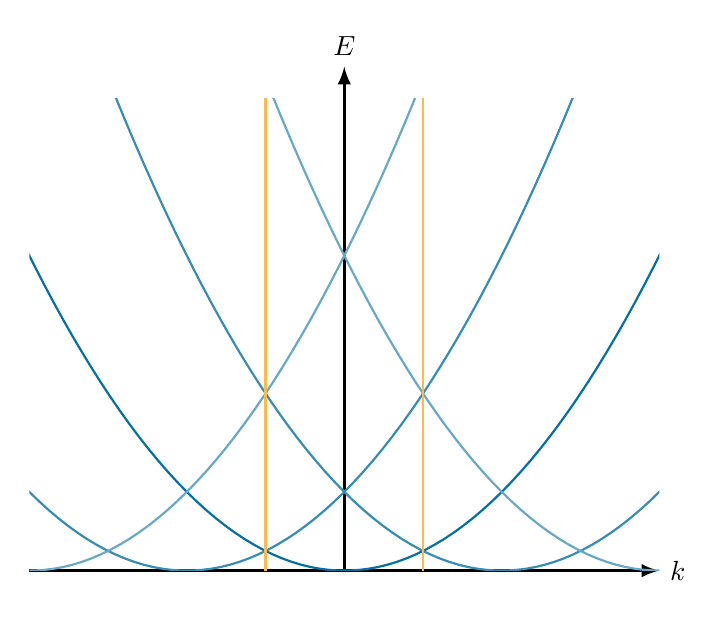
\begin{tikzpicture}
            \draw[very thick, ->] (-4, 0) -- (4, 0) node[right] {\(k\)};
            \draw[very thick, ->] (0, 0) -- (0, 6.4) node[above] {\(E\)};
            \begin{scope}
                \clip (-4, 0) rectangle (4, 6);
                \draw[thick, samples=100, domain=-6:6, highlight] plot (\x, \x*\x/4);
                \draw[thick, samples=100, domain=-6:6, highlight!80] plot (\x-2, \x*\x/4);
                \draw[thick, samples=100, domain=-6:6, highlight!80] plot (\x+2, \x*\x/4);
                \draw[thick, samples=100, domain=-6:6, highlight!60] plot (\x-4, \x*\x/4);
                \draw[thick, samples=100, domain=-6:6, highlight!60] plot (\x+4, \x*\x/4);
                \draw[complementary, thick] (1, 0) -- (1, 6);
                \draw[complementary, thick] (-1, 0) -- (-1, 6);
            \end{scope}
        \end{tikzpicture}
        \caption{\(\varepsilon_{\vv{k}}\) and all shifts of \(\varepsilon_{\vv{k}}\) by some lattice vector \(\vv{G}\).}
        \label{fig:electron dispersion relation and G-shifts}
    \end{figure}
    \begin{figure}
        \tikzsetnextfilename{electron-dispersion-relation-and-G-shifts-restricted}
        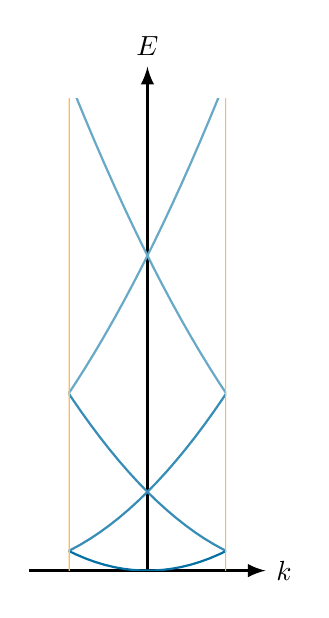
\begin{tikzpicture}
            \draw[very thick, ->] (-1.5, 0) -- (1.5, 0) node[right] {\(k\)};
            \draw[very thick, ->] (0, 0) -- (0, 6.4) node[above] {\(E\)};
            \begin{scope}
                \clip (-1, 0) rectangle (1, 6);
                \draw[thick, samples=100, domain=-6:6, highlight] plot (\x, \x*\x/4);
                \draw[thick, samples=100, domain=-6:6, highlight!80] plot (\x-2, \x*\x/4);
                \draw[thick, samples=100, domain=-6:6, highlight!80] plot (\x+2, \x*\x/4);
                \draw[thick, samples=100, domain=-6:6, highlight!60] plot (\x-4, \x*\x/4);
                \draw[thick, samples=100, domain=-6:6, highlight!60] plot (\x+4, \x*\x/4);
                \draw[complementary, thick] (1, 0) -- (1, 6);
                \draw[complementary, thick] (-1, 0) -- (-1, 6);
            \end{scope}
        \end{tikzpicture}
        \caption{\(\varepsilon_{\vv{k}}\) and all \(\vv{G}\)-shifts of \(\varepsilon_{\vv{k}}\) for some reciprocal lattice vector \(\vv{G}\).}
        \label{fig:restricted electron dispersion relation and all G-shifts}
    \end{figure}
    
    The alternative method, of shifting the parts of \(\varepsilon_{\vv{k}}\) outside of the Brillouin zone by some reciprocal lattice vector such that they are inside the Brillouin zone, is illustrated in \cref{fig:mapping outside BZ into BZ}.
    
    \begin{figure}
        \tikzsetnextfilename{shift-dispersion-relation-into-brillouin-zone}
        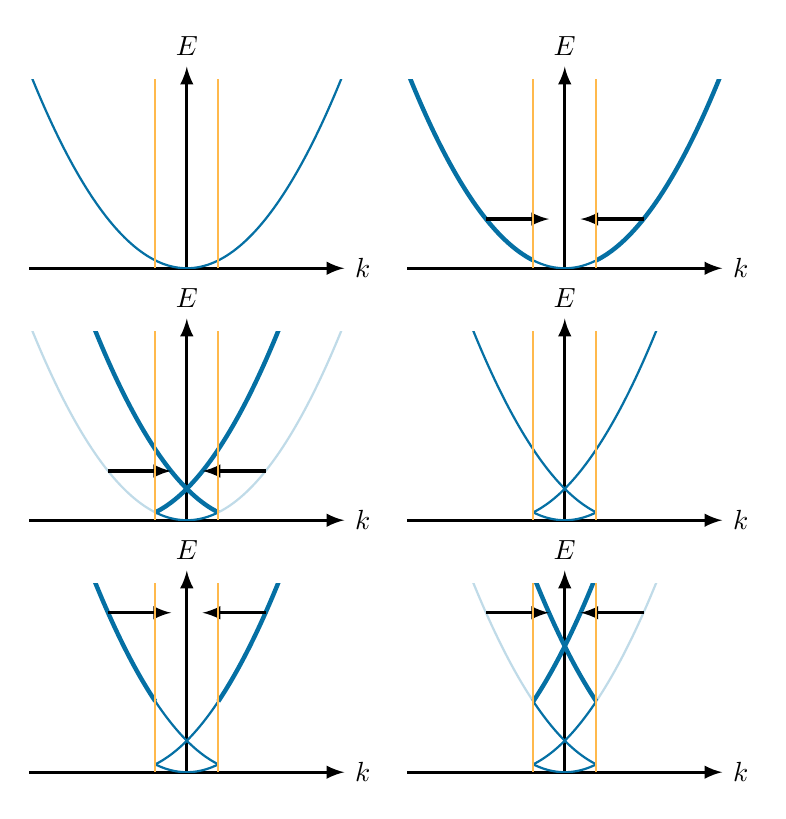
\begin{tikzpicture}[scale=0.4]
            \draw[very thick, ->] (-5, 0) -- (5, 0) node[right] {\(k\)};
            \draw[very thick, ->] (0, 0) -- (0, 6.4) node[above] {\(E\)};
            \begin{scope}
                \clip (-5, 0) rectangle (5, 6);
                \draw[thick, samples=100, domain=-5:5, highlight] plot (\x, \x*\x/4);
            \end{scope}
            \draw[complementary, thick] (1, 0) -- (1, 6);
            \draw[complementary, thick] (-1, 0) -- (-1, 6);
            
            \begin{scope}[xshift=12cm]
                \draw[very thick, ->] (-5, 0) -- (5, 0) node[right] {\(k\)};
                \draw[very thick, ->] (0, 0) -- (0, 6.4) node[above] {\(E\)};
                \begin{scope}
                    \clip (-5, 0) rectangle (5, 6);
                    \draw[thick, samples=100, domain=-5:5, highlight] plot (\x, \x*\x/4);
                    \draw[ultra thick, samples=100, domain=1:5, highlight] plot (\x, \x*\x/4);
                    \draw[ultra thick, samples=100, domain=-5:-1, highlight] plot (\x, \x*\x/4);
                    \draw[->, very thick] (2.5, 2.5^2/4) -- ++ (-2, 0);
                    \draw[->, very thick] (-2.5, 2.5^2/4) -- ++ (2, 0);
                \end{scope}
                \draw[complementary, thick] (1, 0) -- (1, 6);
                \draw[complementary, thick] (-1, 0) -- (-1, 6);
            \end{scope}
            
            \begin{scope}[yshift=-8cm]
                \draw[very thick, ->] (-5, 0) -- (5, 0) node[right] {\(k\)};
                \draw[very thick, ->] (0, 0) -- (0, 6.4) node[above] {\(E\)};
                \begin{scope}
                    \clip (-5, 0) rectangle (5, 6);
                    \draw[thick, samples=100, domain=-1:1, highlight] plot (\x, \x*\x/4);
                    \draw[thick, samples=100, domain=-5:-1, highlight!25] plot (\x, \x*\x/4);
                    \draw[thick, samples=100, domain=1:5, highlight!25] plot (\x, \x*\x/4);
                    \draw[ultra thick, samples=100, domain=1:5, highlight, xshift=-2cm] plot (\x, \x*\x/4);
                    \draw[ultra thick, samples=100, domain=-5:-1, highlight, xshift=2cm] plot (\x, \x*\x/4);
                    \draw[->, very thick] (2.5, 2.5^2/4) -- ++ (-2, 0);
                    \draw[->, very thick] (-2.5, 2.5^2/4) -- ++ (2, 0);
                \end{scope}
                \draw[complementary, thick] (1, 0) -- (1, 6);
                \draw[complementary, thick] (-1, 0) -- (-1, 6);
            \end{scope}
            
            \begin{scope}[xshift=12cm, yshift=-8cm]
                \draw[very thick, ->] (-5, 0) -- (5, 0) node[right] {\(k\)};
                \draw[very thick, ->] (0, 0) -- (0, 6.4) node[above] {\(E\)};
                \begin{scope}
                    \clip (-5, 0) rectangle (5, 6);
                    \draw[thick, samples=100, domain=-1:1, highlight] plot (\x, \x*\x/4);
                    \draw[thick, samples=100, domain=1:5, highlight, xshift=-2cm] plot (\x, \x*\x/4);
                    \draw[thick, samples=100, domain=-5:-1, highlight, xshift=2cm] plot (\x, \x*\x/4);
                \end{scope}
                \draw[complementary, thick] (1, 0) -- (1, 6);
                \draw[complementary, thick] (-1, 0) -- (-1, 6);
            \end{scope}
            
            \begin{scope}[yshift=-16cm]
                \draw[very thick, ->] (-5, 0) -- (5, 0) node[right] {\(k\)};
                \draw[very thick, ->] (0, 0) -- (0, 6.4) node[above] {\(E\)};
                \begin{scope}
                    \clip (-5, 0) rectangle (5, 6);
                    \draw[thick, samples=100, domain=-1:1, highlight] plot (\x, \x*\x/4);
                    \draw[thick, samples=100, domain=1:3, highlight, xshift=-2cm] plot (\x, \x*\x/4);
                    \draw[thick, samples=100, domain=-3:-1, highlight, xshift=2cm] plot (\x, \x*\x/4);
                    \draw[ultra thick, samples=100, domain=3:5, highlight, xshift=-2cm] plot (\x, \x*\x/4);
                    \draw[ultra thick, samples=100, domain=-5:-3, highlight, xshift=2cm] plot (\x, \x*\x/4);
                    \draw[->, very thick] (2.5, {6.75^2/9}) -- ++ (-2, 0);
                    \draw[->, very thick] (-2.5, {6.75^2/9}) -- ++ (2, 0);
                \end{scope}
                \draw[complementary, thick] (1, 0) -- (1, 6);
                \draw[complementary, thick] (-1, 0) -- (-1, 6);
            \end{scope}
            
            \begin{scope}[xshift=12cm, yshift=-16cm]
                \draw[very thick, ->] (-5, 0) -- (5, 0) node[right] {\(k\)};
                \draw[very thick, ->] (0, 0) -- (0, 6.4) node[above] {\(E\)};
                \begin{scope}
                    \clip (-5, 0) rectangle (5, 6);
                    \draw[thick, samples=100, domain=-1:1, highlight] plot (\x, \x*\x/4);
                    \draw[thick, samples=100, domain=1:3, highlight, xshift=-2cm] plot (\x, \x*\x/4);
                    \draw[thick, samples=100, domain=-3:-1, highlight, xshift=2cm] plot (\x, \x*\x/4);
                    \draw[thick, samples=100, domain=3:5, highlight!25, xshift=-2cm] plot (\x, \x*\x/4);
                    \draw[thick, samples=100, domain=-5:-3, highlight!25, xshift=2cm] plot (\x, \x*\x/4);
                    \draw[ultra thick, samples=100, domain=3:5, highlight, xshift=-4cm] plot (\x, \x*\x/4);
                    \draw[ultra thick, samples=100, domain=-5:-3, highlight, xshift=4cm] plot (\x, \x*\x/4);
                    \draw[->, very thick] (2.5, {6.75^2/9}) -- ++ (-2, 0);
                    \draw[->, very thick] (-2.5, {6.75^2/9}) -- ++ (2, 0);
                \end{scope}
                \draw[complementary, thick] (1, 0) -- (1, 6);
                \draw[complementary, thick] (-1, 0) -- (-1, 6);
            \end{scope}
        \end{tikzpicture}
        \caption[Reducing dispersion relations to the first Brillouin zone.]{The process for mapping a dispersion relation outside of the Brillouin zone into the Brillouin zone by mapping parts outside by a reciprocal lattice vector.}
        \label{fig:mapping outside BZ into BZ}
    \end{figure}
    
    In more dimensions we can do exactly the same, although the first method of shifting is much easier to visualise.
    The difference is that instead of parabolas we use paraboloids.
    We then typically plot the intersection of these paraboloids with some plane.
    For example plotting for the \((y,z)\)-plane we get the result shown in \cref{fig:electron bands in two dimensions}.
    To see where the second, higher up parabola comes in see \cref{fig:parabaloids-intersect-plane} which shows how a parabola shifted by a lattice vector perpendicular to the plane intersects the plane to give a higher up parabola.
    
    \begin{figure}
        \tikzsetnextfilename{electron-bands-2d}
        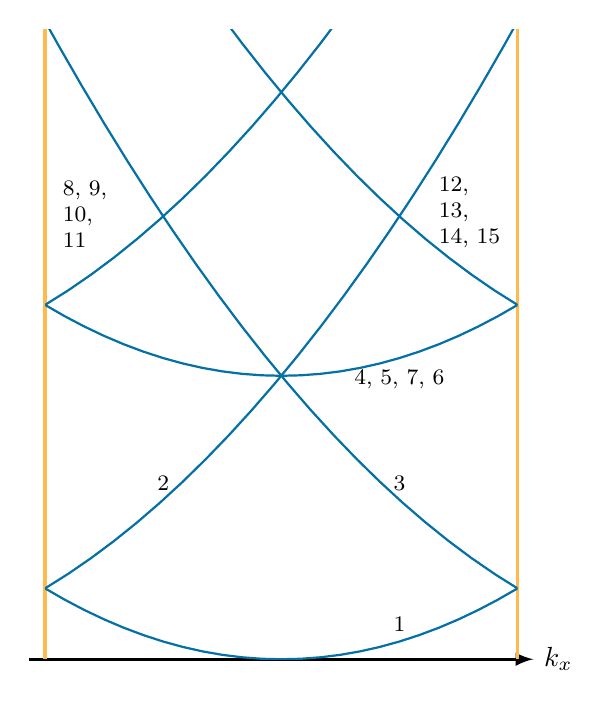
\begin{tikzpicture}
            \draw[->, very thick] (-3.2, 0) -- (3.2, 0) node[right] {\(k_x\)};
            \draw[complementary, very thick] (3, 0) -- ++ (0, 8);
            \draw[complementary, very thick] (-3, 0) -- ++ (0, 8);
            \begin{scope}
                \clip (-3, 0) rectangle (3, 8);
                \draw[highlight, domain=-3:3, thick] plot (\x, \x*\x/10);
                \draw[highlight, domain=3:10, thick] plot (\x-6, \x*\x/10);
                \draw[highlight, domain=-10:-3, thick] plot (\x+6, \x*\x/10);
                \begin{scope}[yshift=3.6cm]
                    \draw[highlight, domain=-3:3, thick] plot (\x, \x*\x/10);
                    \draw[highlight, domain=3:10, thick] plot (\x-6, \x*\x/10);
                    \draw[highlight, domain=-10:-3, thick] plot (\x+6, \x*\x/10);
                \end{scope}
            \end{scope}
            \begin{scope}[font=\footnotesize]
                \node[above] at (1.5, 1.5*1.5/10) {1};
                \node[above] at (-1.5, {(1.5 - 6)^2/10}) {2};
                \node[above] at (1.5, {(1.5 - 6)^2/10}) {3};
                \node[below] at (1.5, 3.8) {4, 5, 7, 6};
                \node[above] at (2.4, 5.1) {\parbox{0.8cm}{\raggedright 12, 13, 14, 15}};
                \node[above] at (-2.4, 5.1) {\parbox{0.75cm}{\raggedright 8, 9, 10, 11}};
            \end{scope}
        \end{tikzpicture}
        \caption{Electron bands in two dimensions.}
        \label{fig:electron bands in two dimensions}
    \end{figure}
    
    \begin{figure}
        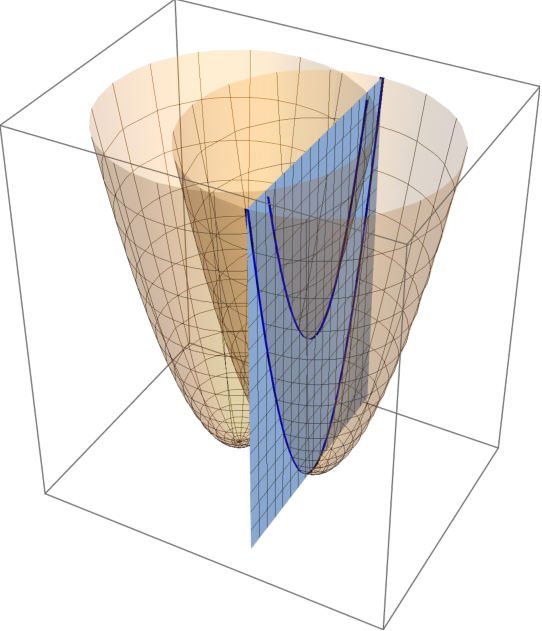
\includegraphics[width=0.8\textwidth]{images/parabolas-from-parabaloids.pdf}
        \caption[Parabaloids intersect plane to give parabolas.]{A paraboloid at the origin and a shifted paraboloid intersect a plane along two parabolas.}
        \label{fig:parabaloids-intersect-plane}
    \end{figure}
    
    Consider the equation for the shifted paraboloids in three dimensions.
    We have
    \begin{equation}
        \varepsilon(\vv{k}) = \frac{\hbar^2}{2m}(\vv{k} + \vv{G})^2 = \frac{\hbar^2}{2m}[(k_x + G_x)^2 + (k_y + G_y)^2 + (k_z + G_y)^2].
    \end{equation}
    We can now go systematically through the lattice vectors and work out all of the paraboloids that we need to consider.
    First we have \(\vv{G} = \vv{0}\), which gives us the base paraboloid
    \begin{equation}
        \varepsilon(\vv{k}) = \frac{\hbar^2}{2m}k^2 = \frac{\hbar^2}{2m}[k_x^2 + k_y^2 + k_z^2].
    \end{equation}
    In the \((k_y, k_z)\)-plane we have \(k_y = k_z = 0\) and so this gives the parabola
    \begin{equation}
        \varepsilon(k_x) = \frac{\hbar^2}{2m}k_x^2.
    \end{equation}
    Then we can consider \(\vv{G} = \vv{a_1^*}\), which points in the \enquote{\(x\)}-direction in reciprocal space.
    For a simple cubic lattice we then have
    \begin{equation}
        \varepsilon(\vv{k}) = \frac{\hbar^2}{2m}(\vv{k} + \vv{a_1^*}) = \frac{\hbar^2}{2m}[(k_x + 2\pi/a)^2 + k_y^2 + k_z^2].
    \end{equation}
    In the \((k_y, k_z)\)-plane we then have
    \begin{equation}
        \varepsilon(\vv{k}) = \frac{\hbar^2}{2m}(k_x + 2\pi/a)^2.
    \end{equation}
    Next we consider \(\vv{G} = \vv{a_2^*}\), we then have
    \begin{equation}
        \varepsilon(\vv{k}) = \frac{\hbar^2}{2m}(\vv{k} + \vv{a_2^*})^2 = \frac{\hbar^2}{2m}[k_x^2 + (k_y + 2\pi/a)^2 + k_z^2].
    \end{equation}
    In the \((k_y, k_z)\)-plane we then have
    \begin{equation}
        \varepsilon(k_x) = \frac{\hbar^2}{2m}[k_x^2 + (2\pi/a)^2].
    \end{equation}
    The case for \(\vv{G} = \vv{a_3^*}\) is the same.
    Repeating this for all \(\vv{G} = v_i\vv{a_i^*}\) for \(v_i\in\integers\) we can build up the results in \cref{tab:G-shifted paraboloids}.
    
    \begin{table}
        \caption{The value of \(\varepsilon\) at \(\vv{k} = \vv{0}\) and \(\vv{k} = k_x\vv{a_1^*}\) for all \(\vv{G}\)-shifts with \(\abs{\vv{G}} \le \sqrt{2}(2\pi/a)\). Taking \(\hbar^2/(2m) = 1\) for simplicity.}
        \label{tab:G-shifted paraboloids}
        \begin{tabular}{llll}\toprule
            Band & \(\vv{G}\) & \(\varepsilon(000)\) & \(\varepsilon(k_x00)\)\\\midrule
            1 & 000 & 0 & \(k_x^2\)\\
            2 & 100 & \((2\pi/a)^2\) & \((k_x + 2\pi/a)^2\)\\
            3 & \(\bar{1}00\) & \((2\pi/a)^2\) & \((k_x - 2\pi/a)^2\)\\
            4--6 & \(010\), \(0\bar{1}0\), \(001\), \(00\bar{1}\) & \((2\pi/a)^2\) & \(k_x^2 + (2\pi/a)^2\)\\
            8--11 & \(110\), \(101\), \(1\bar{1}0\), \(10\bar{1}\) & \(2(2\pi/a)^2\) & \((k_x + 2\pi/a)^2 + (2\pi/a)^2\)\\
            12--15 & \(\bar{1}10\), \(\bar{1}01\), \(\bar{1}\bar{1}0\), \(\bar{1}0\bar{1}\) & \(2(2\pi/a)^2\) & \((k_x - 2\pi/a)^2 + (2\pi/a)^2\)\\
            16--19 & \(011\), \(01\bar{1}\), \(0\bar{1}1\), \(0\bar{1}\bar{1}\) & \(2(2\pi/a)^2\) & \(k_x^2 + 2(2\pi/a)^2\)\\\bottomrule
        \end{tabular}
    \end{table}
    
    \section{Bloch's Theorem}
    The periodicity of a crystal lattice imposes constraints on possible electron wave functions.
    In particular \defineindex{Bloch's theorem} states that all solutions to Schr\"odinger's equation must be of the form
    \begin{equation}
        \psi_{\vv{k}}(\vv{r}) = u_{\vv{k}}(\vv{r})\e^{i\vv{k}\cdot\vv{r}}
    \end{equation}
    where \(u_{\vv{k}}\) is some function with the same periodicity as the lattice.
    This means that \(u_{\vv{k}}(\vv{r} + \vv{T}) = u_{\vv{k}}(\vv{r})\), where \(\vv{T}\) is a translation vector of the lattice.
    
    This result means that the possible one electron wave functions, \(\psi_{\vv{k}}\), are plane waves, \(\e^{i\vv{k}\cdot\vv{r}}\), modulated by periodic functions, \(u_{\vv{k}}\).
    This does \emph{not} mean that the wave functions are periodic.
    
    The consequence of this theorem is that \(\psi_{\vv{k} + \vv{G}}(\vv{r}) = \psi_{\vv{k}}(\vv{r})\) and \(\varepsilon(\vv{k} + \vv{G}) = \varepsilon(\vv{k})\), that is the wave function and energy are periodic in the wave vector for any reciprocal lattice vector, \(\vv{G}\).
    
    Bloch's theorem means that we only need to consider electron states where the wave vectors lie inside the first Brillouin zone.
    For a state with a wave vector, \(\vv{k'}\), outside the first Brillouin zone there is an equivalent state with wave vector \(\vv{k} = \vv{k'} - \vv{G}\) for some suitable reciprocal lattice vector, \(\vv{G}\), such that \(\vv{k}\) is in the first Brillouin zone.
    
    \subsection{Bloch's Theorem in One Dimension}
    Consider a system of \(N\) lattice points arranged in a ring.
    Suppose there is a periodic potential, \(U\), such that \(U(x + a) = U(x)\) where \(x\) is the distance around the ring and \(a\) is the distance between lattice points around the ring.
    The probability density function for an electron must be periodic around the ring, meaning\(\abs{\psi(x + a)}^2 = \abs{\psi(x)}^2\), which is required as the system is invariant under a rotation taking each lattice point to its neighbour.
    This implies that \(\psi(x + a) = C\psi(x)\) where \(C \in \unitary(1)\) is a complex number with unit modulus.
    From this we see that \(\psi\) is almost periodic, it just changes phase.
    
    If we go once around the ring we get back to where we started.
    The only physically reasonable thing to expect is that the wave function takes the same value after going once around the ring, so \(\psi(x + Na) = \psi(x) = C^N\psi(x)\).
    From this we see that \(C = \e^{2\pi s/N}\), where \(s = 0, 1,\dotsc, N-1\).
    That is \(C\) is the \(N\)th root of unity.
    
    The most general solution satisfying these constraints is that
    \begin{equation}
        \psi(x) = u_{k}(x)\e^{i2\pi (x/a)(s/N)}
    \end{equation}
    where the extra factor of \(x/a\) allows us to consider positions between lattice points.
    Here \(u_k\) is some periodic function such that \(u_k(x) = u_k(x + a)\).
    We identify \(k = 2\pi s/(Na) = 2\pi/L\) where \(L\) is the circumference of the ring.
    We see that we get periodic wave vectors.
    
    \subsubsection{A Comment on the Wave Vector}
    The wave vector, \(\vv{k}\), labels a Bloch wave function, that is \(\vv{k}\) is a quantum number.
    In the free electron limit \(\hbar\vv{k}\) is the linear momentum.
    In the non-free electron case (i.e. reality) \(\hbar\vv{k}\) is \emph{not} the linear momentum.
    Instead we call \(\hbar\vv{k}\) the crystal momentum.
    The wave vector plays the same role as for phonons, for example, it appears in the scattering of an electron by some phonon:
    \begin{equation}
        \vv{k}_{\mathrm{incident}} + \vv{q}_{\mathrm{phonon}} = \vv{k}_{\mathrm{final}} + \vv{G}.
    \end{equation}
    
    \section{Schr\"odinger Equation for a Periodic Potential}
    Consider a periodic crystal potential, \(U\), we continue to make the independent electron approximation and as such \(U\) accounts for the ions and the other electrons and we only need to solve the Schr\"odinger equation for a single electron.
    For simplicity we work in one dimension, but higher dimension cases aren't that different.
    
    Consider some general wave vector, \(\vv{k}\), anywhere in the first Brillouin zone.
    The crystal potential is periodic and as such we can expand it as a Fourier series:
    \begin{equation}
        U(x) = \sum_{G} U_G \e^{iGx}.
    \end{equation}
    Since the potential is a real function it can be shown that \(U_{-G} = U_G^*\).
    
    The Schr\"odinger equation, \(\hamiltonian\psi = \varepsilon\psi\), then takes the form
    \begin{equation}
        \left( \frac{\operator{p}^2}{2m} + U(x) \right)\psi(x) = \left( \frac{\operator{p}^2}{2m} + \sum_G U_G\e^{iGx} \right)\psi(x) = \varepsilon\psi(x).
    \end{equation}
    
    We now express the electron wave function as a Fourier \emph{transform}, not series, accounting for the fact that the transform variable, \(k\), is discrete, since \(k = 2\pi s/L\) for \(s \in \integers\), where \(L = Na\) is the length of the crystal.
    This means we write \(\psi\) as
    \begin{equation}
        \psi(x) = \sum_{k} C_k\e^{ikx}.
    \end{equation}
    Since we are summing over the relatively dense set of wave vectors, rather than over reciprocal lattice vectors, \(G\), this does not yield a periodic wave function.
    We also include wave vectors outside of the first Brillouin zone.
    
    Considering the first term of the Schr\"odinger equation we now have
    \begin{equation}
        \frac{\operator{p}^2}{2m}\psi(x) = \frac{\hbar^2}{2m}\diff[2]{\psi}{x} = -\frac{\hbar^2}{2m}\sum_{k}k^2C_k\e^{ikx}.
    \end{equation}
    The second term gives
    \begin{equation}
        \sum_G\sum_k U_GC_k\e^{i(G + k)x}.
    \end{equation}
    Renaming \(k\) to \(k'\) in this term and putting the terms together the Schr\"odinger equation becomes
    \begin{equation}
        \sum_{k} \frac{\hbar^2}{2m}k^2C_k\e^{ikx} + \sum_G\sum_k U_GC_{k'}\e^{i(k' + G)x} = \sum_{k} \varepsilon C_k\e^{ikx}.
    \end{equation}
    We can rewrite second term to be in terms of \(k = k' + G\) and we get
    \begin{equation}
        \sum_k \frac{\hbar^2}{2m} k^2C_k\e^{ikx} + \sum_G\sum_k U_GC_{k-G}\e^{ikx} = \sum_k \varepsilon C_k\e^{ikx}.
    \end{equation}
    Each Fourier component, \(\e^{ikx}\), must have the same coefficient on either side of the equation and so we conclude that
    \begin{equation}
        \frac{\hbar^2}{2m}k^2C_k + \sum_G U_GC_{k-G} = \varepsilon C_k
    \end{equation}
    for all \(k\).
    
    Defining \(\lambda_k \coloneqq \hbar^2k^2/(2m)\) lets us write this as
    \begin{equation}
        (\lambda_k - \varepsilon)C_k + \sum_G U_GC_{k - G} = 0.
    \end{equation}
    We call this the \defineindex{central equation}.
    
    We see that we end up with a system of simultaneous linear equations for \(C_k\).
    We can write this with matrices and the problem of finding the values of \(C_k\) becomes a matrix inversion problem.
    This can then be done efficiently on a computer.
    To do so we obviously need to truncate the sums at some finite number of terms, keeping enough terms that we achieve the desired accuracy, but not so many that the computation takes too long.
    
    We can reasonably compute the sums keeping enough terms that the limiting factor in accuracy is not the number of terms but the independent electron approximation.
    Overcoming this barrier is an area of active research.
    Currently techniques include accounting for some electron interaction in the potential, this is done in the frame work of density functional theory, but this is beyond the scope of this course.
    
    \subsection{Bloch's Theorem Again}
    We can \enquote{prove} Bloch's theorem from the central equation.
    We do not, in general, expect that the wave function, \(\psi\), given by
    \begin{equation}
        \psi(x) = \sum_k C_k\e^{ikx},
    \end{equation}
    will be periodic with the crystal lattice, which is fine, since the wave function doesn't need to be periodic to satisfy Bloch's theorem.
    
    The central equation couples \(C_k\) to \(C_{k + nG}\) for \(n \in \integers\).
    We can write the wave function as
    \begin{equation}
        \psi_k(x) = \sum_G C_{k-G}\e^{i(k-G)x},
    \end{equation}
    for some fixed wave vector \(k\).
    Rearranging this we have
    \begin{equation}
        \psi_k(x) = \e^{ikx} \sum_G \e^{-i G x} = \e^{ikx}u_{k(x)}
    \end{equation}
    here we identify \(u_{k}(x)\) as the sum and we know that this has the periodicity of the lattice since we can also identify it as the Fourier \emph{series} of some function, \(u_k\).
    Hence \(\psi_k(x) = u_k(x)\e^{ikx}\) is of the form expected by Bloch's theorem.
    
    \section{Fermi Surfaces}
    The \define{Fermi surface}\index{Fermi!surface} is a surface in reciprocal space which is the boundary occupied and unoccupied states.
    We can think of it as the surface of constant energy with \(\varepsilon(\vv{k}) = \varepsilon_{\fermi}\).
    Fermi surfaces are important since electronic properties depend on electron states near the Fermi surface, with near typically meaning within \(\boltzmann T\), since these are the only states between which electrons can be thermally excited.
    
    We can express many important electronic properties as integrals over the Fermi surface, \(\mathrm{FS}\), for example the electrical conductivity, \(\sigma\):
    \begin{equation}
        \sigma \propto \int_{\mathrm{FS}} \frac{v_x^2(\vv{k})}{v(\vv{k})}\tau(\vv{k}) \dd{f_{\mathrm{FS}}}
    \end{equation}
    where \(v\) is the electron velocity, \(\tau\) the scattering time, and we assume an electric field in the \(x\)-direction.
    The electronic density of states can similarly be expressed as a Fermi surface integral, and the electronic density of states appears in many more properties, such as the electronic heat capacity,
    \begin{equation}
        C_{\mathrm{el}} = \frac{1}{3}\pi^2D(\varepsilon_{\fermi})\boltzmann^2 T.
    \end{equation}
    
    So far we have thought of the Fermi surface as a sphere, of radius \(k_{\fermi}\).
    This is valid for monovalent metals.
    For polyvalent metals the Fermi surface is more complicated.
    In particular it starts to extend beyond the first Brillouin zone.
    
    Consider the example of a square unit cell in two dimensions with lattice parameter \(a\).
    In a crystal with \(N\) unit cells there are \(2N\) states in the square Brillouin zone, two for each allowed value of \(k\), of which there are \(N\).
    
    For a monovalent crystal there is one valence electron per atom and there are \(N\) electrons in the crystal, hence
    \begin{equation}
        \pi k_{\fermi}^2 = \frac{1}{2}\left( \frac{2\pi}{a} \right)^2 \implies k_{\fermi} = \sqrt{\frac{2}{\pi}} \frac{\pi}{a}.
    \end{equation}
    The left hand side here being the area contained by the Fermi surface (which is a circle in the two-dimensional, square unit cell case).
    The right hand side is half of the area of the unit cell in reciprocal space, since the unit cell contains \(2N\) electron states, and we have \(N\) electrons.
    
    \begin{figure}
        \tikzsetnextfilename{fermi-circles}
        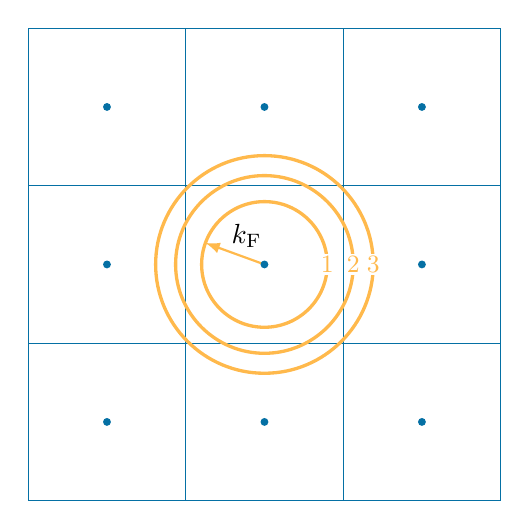
\begin{tikzpicture}
            \draw[highlight, step=2] (0, 0) grid (6, 6);
            \draw[->, thick, complementary, text=black] (3, 3) -- ++ (160:{sqrt(2/pi)}) node[pos=0.3, above] {\(k_{\fermi}\)};
            \foreach \i in {1, 3, 5} {
                \foreach \j in {1, 3, 5} {
                    \fill[highlight] (\i, \j) circle [radius = 0.05cm];
                }
            }
            \foreach \i in {1, 2, 3} {
                \pgfmathsetmacro{\radius}{sqrt(2*\i/pi)}
                \draw[complementary, very thick] (3, 3) circle [radius = \radius];
                \node[fill=white, font=\small, inner sep=1pt, text=complementary] at (3 + \radius, 3) {\i};
            }
        \end{tikzpicture}
        \caption[Square unit cell Fermi surfaces]{The Fermi surfaces for a square unit cell are circles, for divalent and trivalent crystals they extend beyond the first Brillouin zone.}
    \end{figure}
    
    For a divalent crystal we have
    \begin{equation}
        \pi k_{\fermi}^2 = \left( \frac{2\pi}{a} \right)^2 \implies k_{\fermi} = \sqrt{\frac{4}{\pi}}\frac{\pi}{a}.
    \end{equation}
    For a trivalent crystal we have
    \begin{equation}
        \pi k_{\fermi}^2 = \frac{3}{2} \left( \frac{2\pi}{a} \right)^2 \implies k_{\fermi} = \sqrt{\frac{6}{\pi}}\frac{\pi}{a}.
    \end{equation}
    
    In reciprocal space the Brillouin zone has side length \(2\pi/a\), and so any value of \(k_{\fermi}\) greater than \(\pi/a\) is going to extend beyond the first Brillouin zone.
    For the monovalent case \(\sqrt{2/\pi} \approx 0.4\), so the Fermi surface is entirely within the first Brillouin zone.
    For the divalent case \(\sqrt{4/\pi} \approx 0.56\), so the Fermi surface extends outside the first Brillouin zone.
    
    We have seen that every wave vector outside of the first Brillouin zone is equivalent to another wave vector inside the first Brillouin zone.
    This means we can map the Fermi surface outside the first Brillouin zone back into the first Brillouin zone.
    This is what makes the Fermi surfaces of polyvalent crystals more complicated.
    
    \begin{figure}
        \begin{subfigure}{0.7\textwidth}
            \centering
            \tikzsetnextfilename{extended-zone-scheme}
            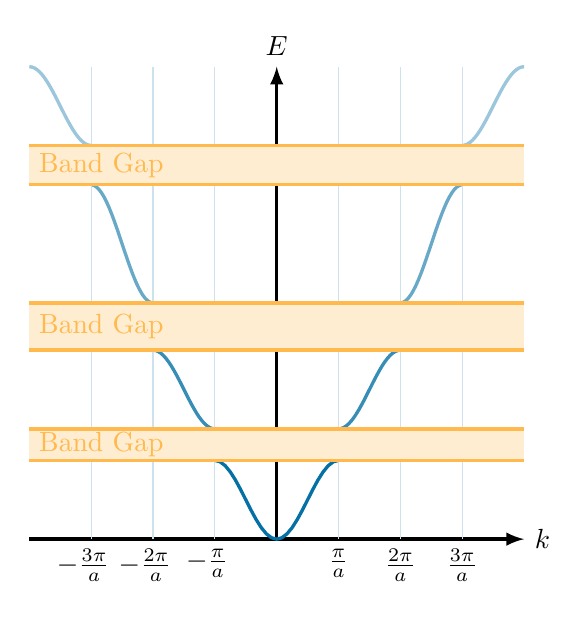
\begin{tikzpicture}[xscale=0.5]
                \draw[->, very thick] (-2*pi, 0) -- (2*pi, 0) node[right] {\(k\)};
                \draw[->, very thick] (0, 0) -- (0, 6) node[above] {\(E\)};
                \begin{scope}[very thick]
                    \draw[domain=-pi/2:pi/2, highlight] plot (\x, {sin(\x r)^2});
                    \draw[domain=pi/2:pi, highlight!80] plot (\x, {cos(\x r)^2 + 1.4});
                    \draw[domain=-pi/2:-pi, highlight!80] plot (\x, {cos(\x r)^2 + 1.4});
                    \draw[domain=pi:3*pi/2, highlight!60] plot (\x, {1.5*sin(\x r)^2 + 3});
                    \draw[domain=-pi:-3*pi/2, highlight!60] plot (\x, {1.5*sin(\x r)^2 + 3});
                    \draw[domain=3*pi/2:2*pi, highlight!40] plot (\x, {cos(\x r)^2 + 5});
                    \draw[domain=-3*pi/2:-2*pi, highlight!40] plot (\x, {cos(\x r)^2 + 5});
                \end{scope}
                \foreach \x in {1, 2, 3, -1, -2, -3} {
                    \draw[highlight!20] (\x * pi / 2, 0) -- ++ (0, 6);
                    \ifnum \x>0
                    \ifnum \x=1
                    \node[below] at (\x * pi / 2, 0) {\(\frac{\pi}{a}\)};
                    \else
                    \node[below] at (\x * pi / 2, 0) {\(\frac{\x\pi}{a}\)};
                    \fi
                    \else
                    \ifnum \x=-1
                    \node[below] at (\x * pi / 2 - 0.2, 0) {\(-\frac{\pi}{a}\)};
                    \else
                    \node[below] at (\x * pi / 2 - 0.2, 0) {\(-\frac{\pgfmathparse{int(-\x)}\pgfmathresult\pi}{a}\)};
                    \fi
                    \fi
                }
                \fill[complementary!25] (-2*pi, 1) rectangle (2*pi, 1.4);
                \fill[complementary!25] (-2*pi, 2.4) rectangle (2*pi, 3);
                \fill[complementary!25] (-2*pi, 4.5) rectangle (2*pi, 5);
                \foreach \y in {1, 1.4, 2.4, 3, 4.5, 5} {
                    \draw[very thick, complementary] (-2*pi, \y) -- (2*pi, \y);
                }
                \foreach \y in {1.2, 2.7, 4.75} {
                    \node[right, complementary] at (-2*pi, \y) {Band Gap};
                }
            \end{tikzpicture}
            \caption{Extended zone scheme.}
        \end{subfigure}
        \begin{subfigure}{0.2\textwidth}
            \centering
            \tikzsetnextfilename{reduced-zone-scheme}
            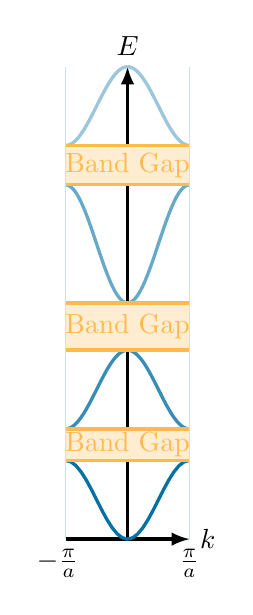
\begin{tikzpicture}[xscale=0.5]
                \draw[->, very thick] (-pi/2, 0) -- (pi/2, 0) node[right] {\(k\)};
                \draw[->, very thick] (0, 0) -- (0, 6) node[above] {\(E\)};
                
                \begin{scope}[very thick]
                    \draw[domain=-pi/2:pi/2, highlight] plot (\x, {sin(\x r)^2});
                    \draw[domain=pi/2:pi, highlight!80, xshift=-3.1415cm] plot (\x, {cos(\x r)^2 + 1.4});
                    \draw[domain=-pi/2:-pi, highlight!80, xshift=3.1415cm] plot (\x, {cos(\x r)^2 + 1.4});
                    \draw[domain=pi:3*pi/2, highlight!60, xshift=-3.1415cm] plot (\x, {1.5*sin(\x r)^2 + 3});
                    \draw[domain=-pi:-3*pi/2, highlight!60, xshift=3.1415cm] plot (\x, {1.5*sin(\x r)^2 + 3});
                    \draw[domain=3*pi/2:2*pi, highlight!40, xshift=-2*3.1415cm] plot (\x, {cos(\x r)^2 + 5});
                    \draw[domain=-3*pi/2:-2*pi, highlight!40, xshift=2*3.1415cm] plot (\x, {cos(\x r)^2 + 5});
                \end{scope}
                
                \fill[complementary!25] (-pi/2, 1) rectangle (pi/2, 1.4);
                \fill[complementary!25] (-pi/2, 2.4) rectangle (pi/2, 3);
                \fill[complementary!25] (-pi/2, 4.5) rectangle (pi/2, 5);
                \foreach \y in {1, 1.4, 2.4, 3, 4.5, 5} {
                    \draw[very thick, complementary] (-pi/2, \y) -- (pi/2, \y);
                }
                \foreach \y in {1.2, 2.7, 4.75} {
                    \node[complementary] at (0, \y) {Band Gap};
                }
                \node[below] at (pi/2, 0) {\(\frac{\pi}{a}\)};
                \node[below] at (-pi/2 - 0.2, 0) {\(-\frac{\pi}{a}\)};
                \draw[highlight!20] (pi/2, 0) -- ++ (0, 6);
                \draw[highlight!20] (-pi/2, 0) -- ++ (0, 6);
            \end{tikzpicture}
            \caption{Reduced zone scheme.}
        \end{subfigure}
        \begin{subfigure}{\textwidth}
            \centering
            \tikzsetnextfilename{periodic-zone-scheme}
            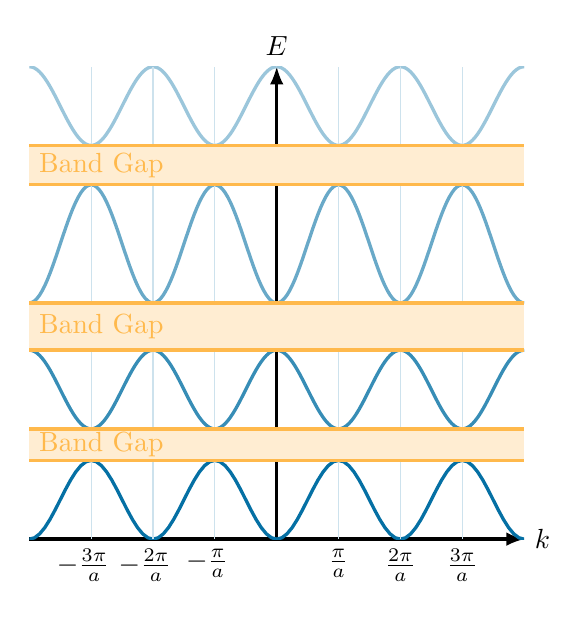
\begin{tikzpicture}[xscale=0.5]
                \draw[->, very thick] (-2*pi, 0) -- (2*pi, 0) node[right] {\(k\)};
                \draw[->, very thick] (0, 0) -- (0, 6) node[above] {\(E\)};
                \begin{scope}
                    \clip (-2*pi, 0) rectangle (2*pi, 6);
                    \foreach \xshift in {0, 3.1415, 2*3.1415, -3.1415, -2*3.1415} {
                        \begin{scope}[very thick, xshift=\xshift cm]
                            \draw[domain=-pi/2:pi/2, highlight] plot (\x, {sin(\x r)^2});
                            \draw[domain=pi/2:pi, highlight!80, xshift=-3.1415cm] plot (\x, {cos(\x r)^2 + 1.4});
                            \draw[domain=-pi/2:-pi, highlight!80, xshift=3.1415cm] plot (\x, {cos(\x r)^2 + 1.4});
                            \draw[domain=pi:3*pi/2, highlight!60, xshift=-3.1415cm] plot (\x, {1.5*sin(\x r)^2 + 3});
                            \draw[domain=-pi:-3*pi/2, highlight!60, xshift=3.1415cm] plot (\x, {1.5*sin(\x r)^2 + 3});
                            \draw[domain=3*pi/2:2*pi, highlight!40, xshift=-2*3.1415cm] plot (\x, {cos(\x r)^2 + 5});
                            \draw[domain=-3*pi/2:-2*pi, highlight!40, xshift=2*3.1415cm] plot (\x, {cos(\x r)^2 + 5});
                        \end{scope}
                    }
                \end{scope}
                \foreach \x in {1, 2, 3, -1, -2, -3} {
                    \draw[highlight!20] (\x * pi / 2, 0) -- ++ (0, 6);
                    \ifnum \x>0
                    \ifnum \x=1
                    \node[below] at (\x * pi / 2, 0) {\(\frac{\pi}{a}\)};
                    \else
                    \node[below] at (\x * pi / 2, 0) {\(\frac{\x\pi}{a}\)};
                    \fi
                    \else
                    \ifnum \x=-1
                    \node[below] at (\x * pi / 2 - 0.2, 0) {\(-\frac{\pi}{a}\)};
                    \else
                    \node[below] at (\x * pi / 2 - 0.2, 0) {\(-\frac{\pgfmathparse{int(-\x)}\pgfmathresult\pi}{a}\)};
                    \fi
                    \fi
                }
                \fill[complementary!25] (-2*pi, 1) rectangle (2*pi, 1.4);
                \fill[complementary!25] (-2*pi, 2.4) rectangle (2*pi, 3);
                \fill[complementary!25] (-2*pi, 4.5) rectangle (2*pi, 5);
                \foreach \y in {1, 1.4, 2.4, 3, 4.5, 5} {
                    \draw[very thick, complementary] (-2*pi, \y) -- (2*pi, \y);
                }
                \foreach \y in {1.2, 2.7, 4.75} {
                    \node[right, complementary] at (-2*pi, \y) {Band Gap};
                }
            \end{tikzpicture}
            \caption{Periodic Zone Scheme}
        \end{subfigure}
        \caption[Reduced dispersion relations.]{Different ways of viewing dispersion relations. In one dimension we can map an extended zone scheme into the first Brillouin zone by shifting by suitable multiples of \(2\pi/a\), giving the reduced zone scheme. We can then extend this to all space by extending it periodically.}
    \end{figure}

    \section{Higher Order Brillouin Zones}
    So far in this course we have considered only the first Brillouin zone, which we have simply been calling \emph{the} Brillouin zone much of the time.
    Recall how we constructed this, using the Wigner--Seitz method, see \cref{sec:wigner-seitz cells} for details.
    Essentially we create lines between lattice points, take the perpendicular bisectors, and then the smallest volume these enclose gives us our cell.
    In doing so we end up with bisectors that don't bound the first cell, instead we can use these to make a slightly larger, no longer primitive cell.
    We call the area in this cell, but not the first Brillouin zone, the second Brillouin zone.
    We can then do something similar to define the third Brillouin zone and so on.
    This is demonstrated in \cref{fig:higher order Brillouin zones}.
    
    It is often easier to consider the alternative definition of the \(n\)th Brillouin zone, that a point, \(\vv{k}\), is in the \(n\)th Brillouin zone if the condition \(\abs{\vv{k}} < \abs{\vv{k} - \vv{G}}\) fails for exactly \(n - 1\) reciprocal lattice vectors, \(\vv{G}\).
    That is that \(\vv{k}\) is closer to the origin than it is to all but \(n - 1\) lattice points.
    This is equivalent to the perpendicular bisector definition since moving across a perpendicular bisector means changing which of the two lattice points the point is closes to.
    
    Each higher order Brillouin zone covers the same wave vectors as the first Brillouin zone, just shifted by some reciprocal lattice vector.
    This means that each Brillouin zone has the same volume.
    We can see this by imagining cutting up the Brillouin zones to fit in the first Brillouin zone.
    See \cref{fig:brillouin zone area}.
    
    \begin{figure}
        \begin{subfigure}{0.4\textwidth}
            \centering
            \tikzsetnextfilename{square-cell-first-brillouin-zone}
            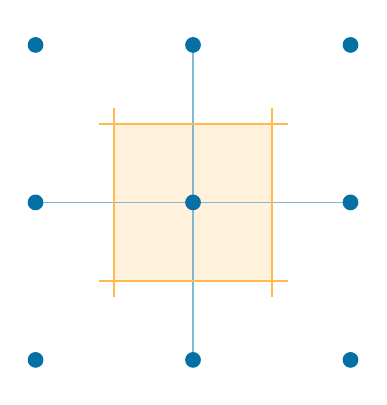
\begin{tikzpicture}
                \fill[complementary!20] (-1, -1) rectangle (1, 1);
                \draw[highlight!50] (-2, 0) -- (2, 0);
                \draw[highlight!50] (0, -2) -- (0, 2);
                \draw[thick, complementary] (-1, 1.2) -- (-1, -1.2);
                \draw[thick, complementary] (1, 1.2) -- (1, -1.2);
                \draw[thick, complementary] (-1.2, 1) -- (1.2, 1);
                \draw[thick, complementary] (-1.2, -1) -- (1.2, -1);
                
                \foreach \i in {-2, 0, 2} {
                    \foreach \j in {-2, 0, 2} {
                        \fill[highlight] (\i, \j) circle [radius = 0.1cm];
                    }
                }
                % make same height as next figure so they line up next to each other
                \draw[white] ($(0, -2) + (-45:0.3)$) -- ++ (0.01, 0);
                \draw[white] ($(0, 2) + (45:0.3)$) -- ++ (0.01, 0);
            \end{tikzpicture}
            \caption{Constructing the first Brillouin zone for a square unit cell.}
        \end{subfigure}
        \begin{subfigure}{0.4\textwidth}
            \centering
            \tikzsetnextfilename{square-cell-second-brillouin-zone}
            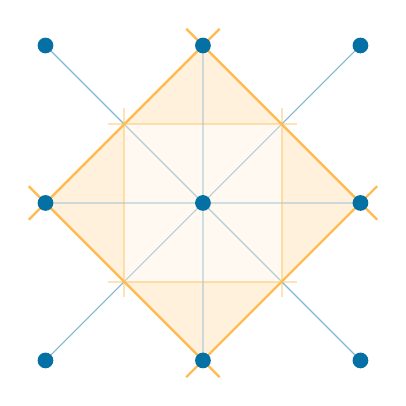
\begin{tikzpicture}
                \draw[highlight!50] (-2, -2) -- (2, 2);
                \draw[highlight!50] (-2, 2) -- (2, -2);
                \fill[complementary!20] (-1, 1) -- (1, 1) -- (0, 2) -- cycle;
                \fill[complementary!20] (1, 1) -- (1, -1) -- (2, 0) -- cycle;
                \fill[complementary!20] (1, -1) -- (-1, -1) -- (0, -2) -- cycle;
                \fill[complementary!20] (-1, -1) -- (-1, 1) -- (-2, 0) -- cycle;
                \draw[thick, complementary] ($(-2, 0) + (-135:0.3)$) -- ($(0, 2) + (45:0.3)$);
                \draw[thick, complementary] ($(0, 2) + (135:0.3)$) -- ($(2, 0) + (-45:0.3)$);
                \draw[thick, complementary] ($(2, 0) + (45:0.3)$) -- ($(0, -2) + (-135:0.3)$);
                \draw[thick, complementary] ($(0, -2) + (-45:0.3)$) -- ($(-2, 0) + (135:0.3)$);
                
                \begin{scope}[opacity=0.4]
                    \fill[complementary!20] (-1, -1) rectangle (1, 1);
                    \draw[highlight!50] (-2, 0) -- (2, 0);
                    \draw[highlight!50] (0, -2) -- (0, 2);
                    \draw[thick, complementary] (-1, 1.2) -- (-1, -1.2);
                    \draw[thick, complementary] (1, 1.2) -- (1, -1.2);
                    \draw[thick, complementary] (-1.2, 1) -- (1.2, 1);
                    \draw[thick, complementary] (-1.2, -1) -- (1.2, -1);
                \end{scope}
                
                \foreach \i in {-2, 0, 2} {
                    \foreach \j in {-2, 0, 2} {
                        \fill[highlight] (\i, \j) circle [radius = 0.1cm];
                    }
                }
            \end{tikzpicture}
            \caption{Constructing the second Brillouin zone for a square unit cell.}
        \end{subfigure}
        \begin{subfigure}{0.8\textwidth}
            \centering
            \tikzsetnextfilename{square-cell-third-brillouin-zone}
            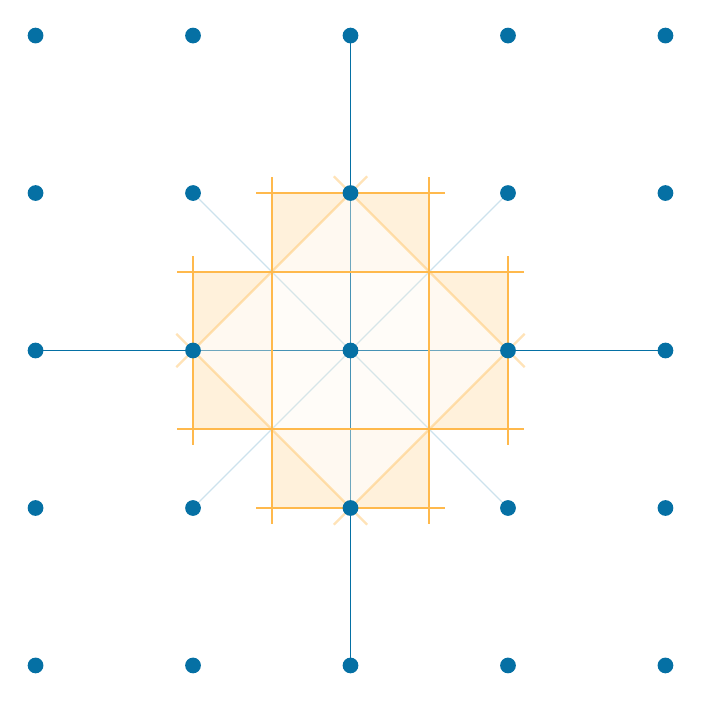
\begin{tikzpicture}
                \draw[highlight] (0, 4) -- (0, -4);
                \draw[highlight] (4, 0) -- (-4, 0);
                \fill[complementary!20] (0, 2) -- (1, 2) -- (1, 1) -- cycle;
                \fill[complementary!20] (1, 1) -- (2, 1) -- (2, 0) -- cycle;
                \fill[complementary!20] (2, 0) -- (2, -1) -- (1, -1) -- cycle;
                \fill[complementary!20] (1, -1) -- (1, -2) -- (0, -2) -- cycle;
                \fill[complementary!20] (0, -2) -- (-1, -2) -- (-1, -1) -- cycle;
                \fill[complementary!20] (-1, -1) -- (-2, -1) -- (-2, 0) -- cycle;
                \fill[complementary!20] (-2, 0) -- (-2, 1) -- (-1, 1) -- cycle;
                \fill[complementary!20] (-1, 1) -- (-1, 2) -- (0, 2) -- cycle;
                \draw[thick, complementary] (-1.2, 2) -- (1.2, 2);
                \draw[thick, complementary] (-1.2, -2) -- (1.2, -2);
                \draw[thick, complementary] (2, -1.2) -- (2, 1.2);
                \draw[thick, complementary] (-2, -1.2) -- (-2, 1.2);
                
                \begin{scope}[opacity=0.4]
                    \draw[highlight!50] (-2, -2) -- (2, 2);
                    \draw[highlight!50] (-2, 2) -- (2, -2);
                    \fill[complementary!20] (-1, 1) -- (1, 1) -- (0, 2) -- cycle;
                    \fill[complementary!20] (1, 1) -- (1, -1) -- (2, 0) -- cycle;
                    \fill[complementary!20] (1, -1) -- (-1, -1) -- (0, -2) -- cycle;
                    \fill[complementary!20] (-1, -1) -- (-1, 1) -- (-2, 0) -- cycle;
                    \draw[thick, complementary] ($(-2, 0) + (-135:0.3)$) -- ($(0, 2) + (45:0.3)$);
                    \draw[thick, complementary] ($(0, 2) + (135:0.3)$) -- ($(2, 0) + (-45:0.3)$);
                    \draw[thick, complementary] ($(2, 0) + (45:0.3)$) -- ($(0, -2) + (-135:0.3)$);
                    \draw[thick, complementary] ($(0, -2) + (-45:0.3)$) -- ($(-2, 0) + (135:0.3)$);
                    
                    \begin{scope}[opacity=0.2]
                        \fill[complementary!20] (-1, -1) rectangle (1, 1);
                        \draw[highlight!50] (-2, 0) -- (2, 0);
                        \draw[highlight!50] (0, -2) -- (0, 2);
                    \end{scope}
                \end{scope}
                \draw[thick, complementary] (-1, 2.2) -- (-1, -2.2);
                \draw[thick, complementary] (1, 2.2) -- (1, -2.2);
                \draw[thick, complementary] (-2.2, 1) -- (2.2, 1);
                \draw[thick, complementary] (-2.2, -1) -- (2.2, -1);
                
                \foreach \i in {-4, -2, 0, 2, 4} {
                    \foreach \j in {-4, -2, 0, 2, 4} {
                        \fill[highlight] (\i, \j) circle [radius = 0.1cm];
                    }
                }
            \end{tikzpicture}
            \caption{Constructing the third Brillouin zone for a square unit cell. Notice that the construction reuses the perpendicular bisectors that were used in the construction of the first Brillouin zone, as well as new perpendicular bisectors from further away lattice points.}
        \end{subfigure}
        \caption[Higher order Brillouin zones]{Extending the notion of Brillouin zones to higher orders.}
        \label{fig:higher order Brillouin zones}
    \end{figure}
    
    \begin{figure}
        \begin{subfigure}{0.4\textwidth}
            \centering
            \tikzsetnextfilename{second-brillouin-zone-fits-in-first}
            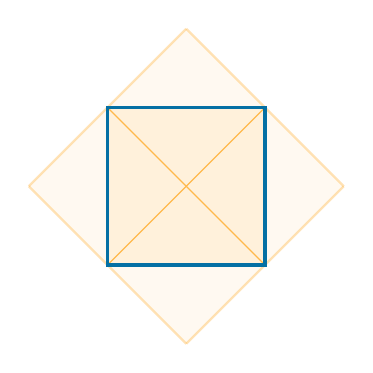
\begin{tikzpicture}
                \begin{scope}[opacity=0.4]
                    \fill[complementary!20] (-1, 1) -- (1, 1) -- (0, 2) -- cycle;
                    \fill[complementary!20] (1, 1) -- (1, -1) -- (2, 0) -- cycle;
                    \fill[complementary!20] (1, -1) -- (-1, -1) -- (0, -2) -- cycle;
                    \fill[complementary!20] (-1, -1) -- (-1, 1) -- (-2, 0) -- cycle;
                    \draw[thick, complementary] (-2, 0) -- (0, 2);
                    \draw[thick, complementary] (0, 2) -- (2, 0);
                    \draw[thick, complementary] (2, 0) -- (0, -2);
                    \draw[thick, complementary] (0, -2) -- (-2, 0);
                \end{scope}
                \fill[complementary!20] (-1, -1) rectangle (1, 1);
                \draw[complementary] (-1, -1) -- (1, 1);
                \draw[complementary] (-1, 1) -- (1, -1);
                \draw[highlight, very thick] (-1, -1) rectangle (1, 1);
            \end{tikzpicture}
            \caption{The second Brillouin zone has the same area as the first.}
        \end{subfigure}
        \begin{subfigure}{0.4\textwidth}
            \centering
            \tikzsetnextfilename{third-Brillouin-zone-fits-in-first}
            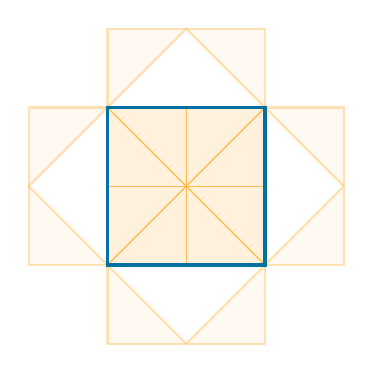
\begin{tikzpicture}
                \begin{scope}[opacity=0.4]
                    \fill[complementary!20] (0, 2) -- (1, 2) -- (1, 1) -- cycle;
                    \fill[complementary!20] (1, 1) -- (2, 1) -- (2, 0) -- cycle;
                    \fill[complementary!20] (2, 0) -- (2, -1) -- (1, -1) -- cycle;
                    \fill[complementary!20] (1, -1) -- (1, -2) -- (0, -2) -- cycle;
                    \fill[complementary!20] (0, -2) -- (-1, -2) -- (-1, -1) -- cycle;
                    \fill[complementary!20] (-1, -1) -- (-2, -1) -- (-2, 0) -- cycle;
                    \fill[complementary!20] (-2, 0) -- (-2, 1) -- (-1, 1) -- cycle;
                    \fill[complementary!20] (-1, 1) -- (-1, 2) -- (0, 2) -- cycle;
                    \draw[thick, complementary] (-1, 2) -- (1, 2) -- (1, 1) -- (2, 1) -- (2, -1) -- (1, -1) -- (1, -2) -- (0, -2) -- (-1, -2) -- (-1, -1) -- (-2, -1) -- (-2, 0) -- (-2, 1) -- (-1, 1) -- cycle;
                    \draw[thick, complementary] (-2, 0) -- (0, 2) -- (2, 0) -- (0, -2) -- cycle;
                \end{scope}
                \fill[complementary!20] (-1, -1) rectangle (1, 1);
                \draw[complementary] (-1, -1) -- (1, 1);
                \draw[complementary] (-1, 1) -- (1, -1);
                \draw[complementary] (0, 1) -- (0, -1);
                \draw[complementary] (1, 0) -- (-1, 0);
                \draw[highlight, very thick] (-1, -1) rectangle (1, 1);
            \end{tikzpicture}
            \caption{The third Brillouin zone has the same area as the first.}
        \end{subfigure}
        \caption[Brillouin zones have the same area]{All Brillouin zones cover the same states, therefore they all have the same area.}
        \label{fig:brillouin zone area}
    \end{figure}
    
    Brillouin zones quickly become rather complicated shapes, even for simple lattices, like the square lattice.
    
    \section{Fermi Surfaces in the First Brillouin Zone}
    We can reduce a Fermi surface that intersects higher order Brillouin zones to a surface entirely in the first Brillouin zone.
    To do so we draw all Fermi surfaces, for each lattice point.
    We then consider only the Fermi surface inside the first Brillouin zone for some given lattice point.
    See \cref{fig:map fermi surface to first brillouin zone}.
    
    \begin{figure}
        \tikzsetnextfilename{map-fermi-surface-to-first-brillouin-zone}
        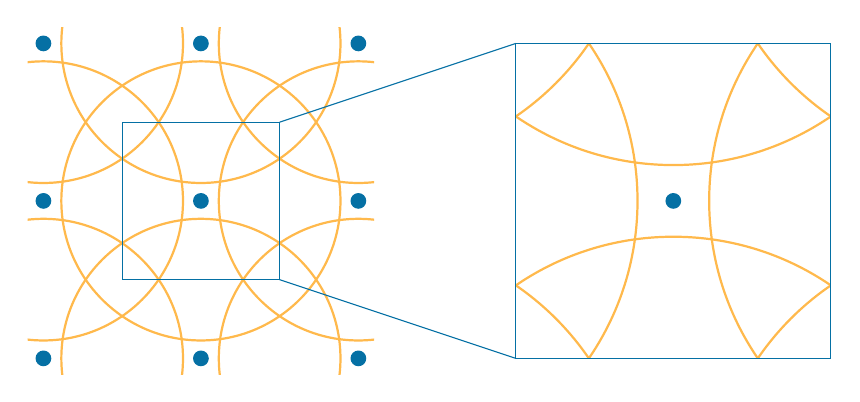
\begin{tikzpicture}
            \begin{scope}
                \clip (-2.2, -2.2) rectangle (2.2, 2.2);
                \foreach \i in {-2, 0, 2} {
                    \foreach \j in {-2, 0, 2} {
                        \fill[highlight] (\i, \j) circle [radius = 0.1cm];
                        \draw[thick, complementary] (\i, \j) circle [radius = sqrt(pi)];
                    }
                }
            \end{scope}
            \draw[highlight] (-1, -1) rectangle (1, 1);
            \begin{scope}[xshift=6cm]
                \begin{scope}
                    \clip (-2, -2) rectangle (2, 2);
                    \fill[highlight] (0, 0) circle [radius = 0.1cm];
                    \foreach \i in {-4, 0, 4} {
                        \foreach \j in {-4, 0, 4} {
                            \draw[thick, complementary] (\i, \j) circle [radius = 2*sqrt(pi)];
                        }
                    }
                \end{scope}
                \draw[highlight] (-2, -2) rectangle (2, 2);
                \draw[highlight] (-5, 1) -- (-2, 2);
                \draw[highlight] (-5, -1) -- (-2, -2);
            \end{scope}
        \end{tikzpicture}
        \caption[Reduced Fermi surface.]{Mapping the Fermi surface to the first Brillouin zone by repeating the Fermi surface with the lattice and then ignoring everything outside of the first Brillouin zone for some given lattice point.}
        \label{fig:map fermi surface to first brillouin zone}
    \end{figure}
    
    Having done this we can then separate the reduced Fermi surface into parts, often called sheets, according to the Brillouin zone that they were in before mapping.
    Doing so we see that none of the Fermi surface comes from the first Brillouin zone, since the circle is entirely outside of the first Brillouin zone.
    The distorted square around the lattice point comes from the second Brillouin zone.
    The third Brillouin zone gives four pointed stars, one point of which is in the first Brillouin zone for each corner.
    The fourth Brillouin zone gives distorted squares on each corner, one quarter of which is in the first Brillouin zone.
    
    \begin{figure}
        \tikzsetnextfilename{mapped-brillouin-zone-domain}
        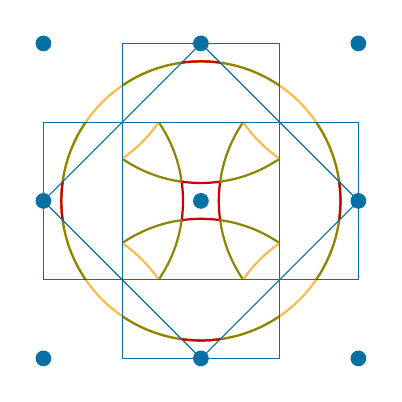
\begin{tikzpicture}
            \begin{scope}
                \clip (-2.2, -2.2) rectangle (2.2, 2.2);
                \draw[thick, complementary] (0, 0) circle [radius = sqrt(pi)];
                \foreach \i in {-2, 0, 2} {
                    \foreach \j in {-2, 0, 2} {
                        \fill[highlight] (\i, \j) circle [radius = 0.1cm];
                    }
                }
            \end{scope}
            \begin{scope}
                \clip (0, 2) -- (1, 2) -- (1, 1) -- (2, 1) -- (2, 0) -- (2, -1) -- (1, -1) -- (1, -2) -- (0, -2) -- (-1, -2) -- (-1, -1) -- (-2, -1) -- (-2, 0) -- (-2, 1) -- (-1, 1) -- (-1, 2) -- cycle;
                \draw[thick, olive] (0, 0) circle [radius = sqrt(pi)];
            \end{scope}
            \begin{scope}
                \clip (0, 2) -- (2, 0) -- (0, -2) -- (-2, 0) -- cycle;
                \draw[thick, positive red] (0, 0) circle [radius = sqrt(pi)];
            \end{scope}
            \begin{scope}
                \clip (-0.258, -0.258)  rectangle (0.258, 0.258);
                \draw[thick, positive red] (0, 2) circle [radius = sqrt(pi)];
                \draw[thick, positive red] (0, -2) circle [radius = sqrt(pi)];
                \draw[thick, positive red] (2, 0) circle [radius = sqrt(pi)];
                \draw[thick, positive red] (-2, 0) circle [radius = sqrt(pi)];
            \end{scope}
            \begin{scope}
                \clip (0.239, 0.239)  rectangle (1, 1);
                \draw[thick, olive] (0, 2) circle [radius = sqrt(pi)];
                \draw[thick, olive] (2, 0) circle [radius = sqrt(pi)];
            \end{scope}
            \begin{scope}
                \clip (0.239, -0.239)  rectangle (1, -1);
                \draw[thick, olive] (0, -2) circle [radius = sqrt(pi)];
                \draw[thick, olive] (2, 0) circle [radius = sqrt(pi)];
            \end{scope}
            \begin{scope}
                \clip (-0.239, -0.239)  rectangle (-1, -1);
                \draw[thick, olive] (0, -2) circle [radius = sqrt(pi)];
                \draw[thick, olive] (-2, 0) circle [radius = sqrt(pi)];
            \end{scope}
            \begin{scope}
                \clip (-0.239, 0.239)  rectangle (-1, 1);
                \draw[thick, olive] (0, 2) circle [radius = sqrt(pi)];
                \draw[thick, olive] (-2, 0) circle [radius = sqrt(pi)];
            \end{scope}
            \begin{scope}[xshift=-2cm, yshift=-2cm]
                \clip (1, 1) rectangle (2, 2);
                \draw[thick, complementary] circle [radius = sqrt(pi)];
            \end{scope}
            \begin{scope}[xshift=-2cm, yshift=2cm]
                \clip (1, -1) rectangle (2, -2);
                \draw[thick, complementary] circle [radius = sqrt(pi)];
            \end{scope}
            \begin{scope}[xshift=2cm, yshift=-2cm]
                \clip (-1, 1) rectangle (-2, 2);
                \draw[thick, complementary] circle [radius = sqrt(pi)];
            \end{scope}
            \begin{scope}[xshift=2cm, yshift=2cm]
                \clip (-1, -1) rectangle (-2, -2);
                \draw[thick, complementary] circle [radius = sqrt(pi)];
            \end{scope}
            \draw[highlight] (-1, -1) rectangle (1, 1);
            \draw[highlight] (0, 2) -- (2, 0) -- (0, -2) -- (-2, 0) -- cycle;
            \draw[highlight] (0, 2) -- (1, 2) -- (1, 1) -- (2, 1) -- (2, 0) -- (2, -1) -- (1, -1) -- (1, -2) -- (0, -2) -- (-1, -2) -- (-1, -1) -- (-2, -1) -- (-2, 0) -- (-2, 1) -- (-1, 1) -- (-1, 2) -- cycle;
        \end{tikzpicture}
        \caption[Fermi surface coloured by Brillouin zone.]{Colour coded reduced Fermi surface based on which Brillouin zone the Fermi surface was mapped from.}
    \end{figure}

    All of this analysis can be applied to other lattices, and in higher dimensions.
    The Brillouin zones, and hence resulting Fermi surfaces, quickly become very complex.
    
    \section{Sharp Edges}
    The Fermi surfaces that we have been drawing have sharp edges.
    This is not the case in reality.
    Modifications to the electron bands due to the actual crystal potential will give much more rounded edges.
    In fact it turns out that real Fermi surfaces will cross Bragg planes, which are the perpendicular planes to the lattice vectors, and hence planes parallel to the edges of the Brillouin zones, at right angles.
    
    Physically we can argue that this is reasonable as follows.
    The group velocity of an electron with wave vector \(\vv{k}\) is given by \(\vv{v_{\mathrm{g}}} = \grad[\vv{k}]\varepsilon(\vv{k})/\hbar\) where \(\varepsilon(\vv{k})\) is the energy dispersion.
    We also know that, by definition, the Fermi surface is a surface of constant energy, \(\varepsilon(\vv{k}) = \varepsilon_{\fermi}\).
    Hence basic multivariable calculus tells us that \(\vv{v_{\mathrm{g}}} \propto \grad[\vv{k}]\varepsilon\) must be perpendicular to the Fermi surface.
    If there is a sharp edge to the Fermi surface then the gradient is undefined at that point and hence the group velocity of the electron is undefined.
    This is not physically reasonable and so we conclude that these sharp edges don't reflect reality.
    Due to the way that the mapping to the first Brillouin zone occurs we see that if the Fermi surface always cuts through the boundaries between Brillouin zones at right angles then the resulting Fermi surface will have no sharp corners after we map it to the first Brillouin zone.
    
    For our purposes we can construct a Fermi surface with sharp corners and simply round off the corners by making the surface cross the Brillouin zone boundary at right angles.
    
    \chapter{Semiconductors}
    \section{Band Structure}
    Recall that for a three dimensional crystal with \(N = N_x N_y N_z\) primitive unit cells with lattice parameters \(L_i = N_i a_i\) the allowed wave vectors have components
    \begin{equation}
        k_i = 0, \pm \frac{2\pi}{L_i}, \pm \frac{4\pi}{L_i}, \dotsc, \frac{N_i\pi}{L_i}.
    \end{equation}
    There are therefore \(N\) distinct wave vectors in the first Brillouin zone, since all states correspond uniquely to a wave vector in the first Brillouin zone.
    Allowing for electron spins there are \(2N\) states in the first Brillouin zone.
    
    \begin{figure}
        \tikzsetnextfilename{model-band-structure}
        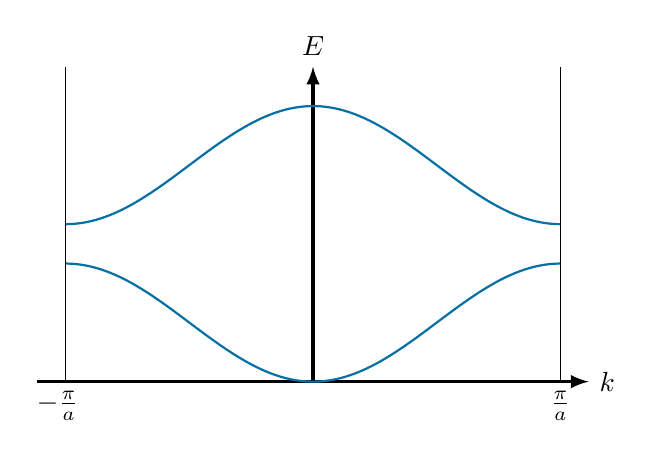
\begin{tikzpicture}
            \draw[very thick, ->] (-3.5, 0) -- (3.5, 0) node[right] {\(k\)};
            \draw[very thick, ->] (0, 0) -- (0, 4) node[above] {\(E\)};
            \draw[domain=-pi:pi, thick, highlight, samples=100] plot (\x, {1.5*sin(\x/2 r)^2});
            \draw[domain=-pi:pi, thick, highlight, samples=100] plot (\x, {1.5*cos(\x/2 r)^2 + 2});
            \draw (pi, 0) -- (pi, 4);
            \draw (-pi, 0) -- (-pi, 4);
            \node[below] at (pi, 0) {\(\frac{\pi}{a}\)};
            \node[below] at (-pi - 0.1, 0) {\(-\frac{\pi}{a}\)};
        \end{tikzpicture}
        \caption{Model band structure.}
        \label{fig:model band structure}
    \end{figure}
    
    Consider the model band structure shown in \cref{fig:model band structure}.
    Depending on the number of electrons per unit cell we get different types of material.
    A monovalent crystal will half fill the first energy band.
    This means that states near the Fermi surface can easily be excited into free states above the Fermi surface.
    This is a metal.
    A divalent crystal with this band structure will completely fill the first energy band.
    It is then not possible to excite electrons across the band gap at reasonable energies.
    This means that an electric field cannot accelerate electrons, hence the material an insulator.
    A trivalent crystal will partially fill the next energy band, so once again it is possible to excite electrons and it will be a metal again.
    See \cref{fig:metal and insulator band structure}.
    
    \begin{figure}
        \begin{subfigure}{0.4\textwidth}
            \centering
            \tikzsetnextfilename{metal-first-band}
            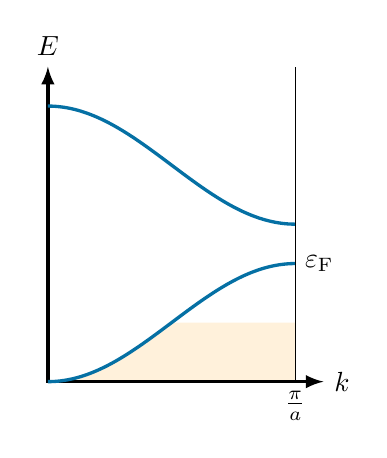
\begin{tikzpicture}
                \fill[domain=0:pi/2, complementary!20] plot (\x, {1.5*sin(\x/2 r)^2}) -- (pi, {1.5*sin(pi/4 r)^2}) -- (pi, 0);
                \node[right] at (pi, 1.5) {\(\varepsilon_{\fermi}\)};
                \draw[very thick, ->] (0, 0) -- (3.5, 0) node[right] {\(k\)};
                \draw[very thick, ->] (0, 0) -- (0, 4) node[above] {\(E\)};
                \draw[very thick] (0, 1) -- (0, 0) -- (1, 0);
                \draw[domain=0:pi, very thick, highlight, samples=100] plot (\x, {1.5*sin(\x/2 r)^2});
                \draw[domain=0:pi, very thick, highlight, samples=100] plot (\x, {1.5*cos(\x/2 r)^2 + 2});
                \draw (pi, 0) -- (pi, 4);
                \node[below] at (pi, 0) {\(\frac{\pi}{a}\)};
            \end{tikzpicture}
            \caption{A metal that partially fills the first electron band.}
        \end{subfigure}
        \begin{subfigure}{0.4\textwidth}
            \centering
            \tikzsetnextfilename{insulator-band-filled}
            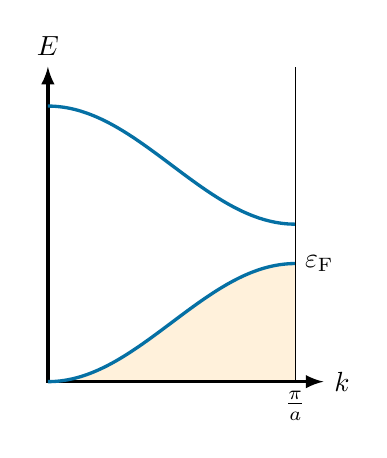
\begin{tikzpicture}
                \fill[domain=0:pi, complementary!20] plot (\x, {1.5*sin(\x/2 r)^2}) -- (pi, 1.5) -- (pi, 0);
                \node[right] at (pi, 1.5) {\(\varepsilon_{\fermi}\)};
                \draw[very thick, ->] (0, 0) -- (3.5, 0) node[right] {\(k\)};
                \draw[very thick, ->] (0, 0) -- (0, 4) node[above] {\(E\)};
                \draw[very thick] (0, 1) -- (0, 0) -- (1, 0);
                \draw[domain=0:pi, very thick, highlight, samples=100] plot (\x, {1.5*sin(\x/2 r)^2});
                \draw[domain=0:pi, very thick, highlight, samples=100] plot (\x, {1.5*cos(\x/2 r)^2 + 2});
                \draw (pi, 0) -- (pi, 4);
                \node[below] at (pi, 0) {\(\frac{\pi}{a}\)};
            \end{tikzpicture}
            \caption{An insulator fills up to a band gap.}
        \end{subfigure}
        \begin{subfigure}{0.8\textwidth}
            \centering
            \tikzsetnextfilename{metal-partially-filled-second-band}
            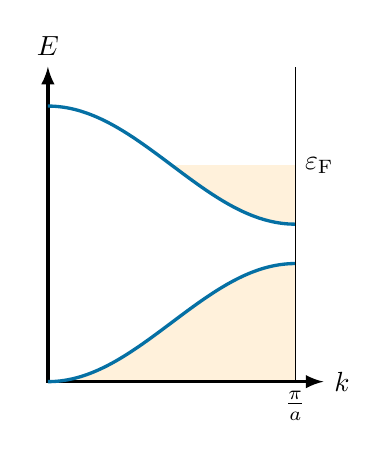
\begin{tikzpicture}
                \fill[domain=0:pi, complementary!20] plot (\x, {1.5*sin(\x/2 r)^2}) -- (pi, 1.5) -- (pi, 0);
                \fill[domain=pi/2:pi, complementary!20] plot (\x, {1.5*cos(\x/2 r)^2 + 2}) -- (pi, 2) -- (pi, {1.5*cos(pi/4 r)^2 + 2});
                \node[right] at (pi, {1.5*cos(pi/4 r)^2 + 2}) {\(\varepsilon_{\fermi}\)};
                \draw[very thick, ->] (0, 0) -- (3.5, 0) node[right] {\(k\)};
                \draw[very thick, ->] (0, 0) -- (0, 4) node[above] {\(E\)};
                \draw[very thick] (0, 1) -- (0, 0) -- (1, 0);
                \draw[domain=0:pi, very thick, highlight, samples=100] plot (\x, {1.5*sin(\x/2 r)^2});
                \draw[domain=0:pi, very thick, highlight, samples=100] plot (\x, {1.5*cos(\x/2 r)^2 + 2});
                \draw (pi, 0) -- (pi, 4);
                \node[below] at (pi, 0) {\(\frac{\pi}{a}\)};
            \end{tikzpicture}
            \caption{A metal that partially fills the second electron band.}
        \end{subfigure}
        \caption[Metal and insulator band structure.]{The same band structure can give metals or insulators, depending on the number of electrons. Since the band structure is symmetric about the origin only positive wave vectors are shown.}
        \label{fig:metal and insulator band structure}
    \end{figure}
    
    Not all divalent crystals are insulators.
    If there is band overlap then instead of filling the first energy band the next band up will be partially filled and the result is that the material will have metallic properties.
    We call such a material a \defineindex{semimetal}.
    See \cref{fig:semimetal band structure}.
    
    \begin{figure}
        \tikzsetnextfilename{semimetal-band-structure}
        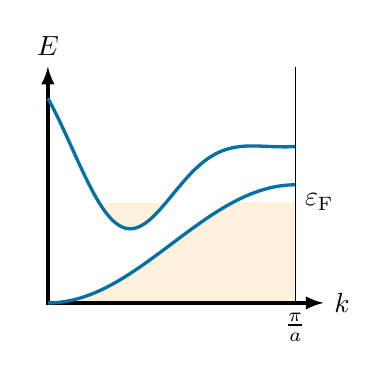
\begin{tikzpicture}
            \fill[domain=0:3*pi/4, complementary!20] plot (\x, {1.5*sin(\x/2 r)^2}) -- (pi, {1.5*sin(3*pi/8 r)^2}) -- (pi, 0);
            \fill[domain=0.65:1.5, complementary!20] plot (\x, {(1.5*cos(\x/2 r)^2 + 2) * (1 - 0.7 * exp(-(\x - 1)^2))});
            \node[right] at (pi, {1.5*sin(3*pi/8 r)^2}) {\(\varepsilon_{\fermi}\)};
            \draw[very thick, ->] (0, 0) -- (3.5, 0) node[right] {\(k\)};
            \draw[very thick, ->] (0, 0) -- (0, 3) node[above] {\(E\)};
            \draw[very thick] (0, 1) -- (0, 0) -- (1, 0);
            \draw[domain=0:pi, very thick, highlight, samples=100] plot (\x, {1.5*sin(\x/2 r)^2});
            \draw[domain=0:pi, very thick, highlight, samples=100] plot (\x, {(1.5*cos(\x/2 r)^2 + 2) * (1 - 0.7 * exp(-(\x - 1)^2))});
            \draw (pi, 0) -- (pi, 3);
            \node[below] at (pi, 0) {\(\frac{\pi}{a}\)};
        \end{tikzpicture}
        \caption[Semimetal band structure.]{The band structure for a semimetal has overlapping bands, so the second band starts to fill up before the first band has finished filling up.}
        \label{fig:semimetal band structure}
    \end{figure}
    
    \section{Semiconductors}
    A \defineindex{semiconductor} is essentially an insulator where the band gap is small enough that a small number of electrons can be excited across the band gap.
    This allows some conductivity, but not as much as a metal.
    Clearly this is temperature dependent since a large amount of the required energy comes from thermal energy.
    What this means is that at sufficiently high temperatures all insulators will become semiconductors.
    This is what we meant by reasonable energy earlier, it's also likely that many insulators will melt before becoming semiconductors.
    On the other hand semiconductors become insulators if they are cooled too much.
    
    There is no agreed upon size of band gap that makes something a semiconductor or an insulator.
    Typically insulators have a band gap greater than about \qtyrange{4}{5}{\electronvolt}, for example diamond has a band gap of \qty{5.5}{\electronvolt} and is definitely an insulator.
    Semiconductors then have smaller band gaps of a couple of electron volts.
    
    \section{Direct and Indirect Band Gaps}
    We can broadly classify semiconductors into two categories, direct and indirect band gaps.
    A \defineindex{direct band gap} has the maxima of the lower band at the same wave vector as the minima of the upper band.
    An \defineindex{indirect band gap} doesn't.
    See \cref{fig:direct and indirect band gaps}.
    
    \begin{figure}
        \begin{subfigure}{0.8\textwidth}
            \centering
            \tikzsetnextfilename{direct-band-gap}
            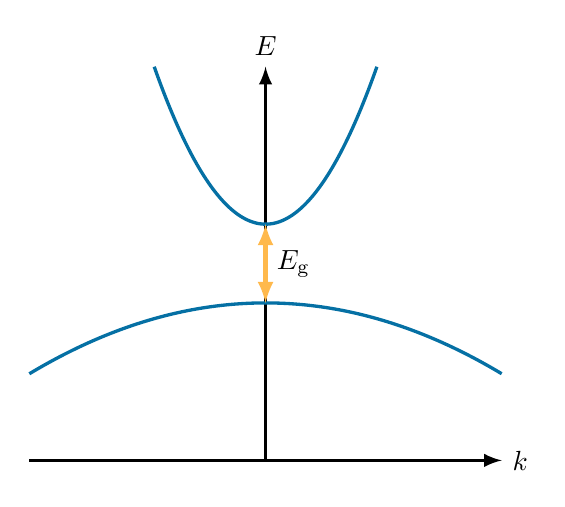
\begin{tikzpicture}
                \draw[very thick, ->] (-3, 0) -- (3, 0) node[right] {\(k\)};
                \draw[very thick, ->] (0, 0) -- (0, 5) node[above] {\(E\)};
                \draw[highlight, very thick, domain=-3:3, samples=100] plot (\x, -0.1*\x*\x+2);
                \draw[highlight, very thick, domain=-1.414:1.414, samples=100] plot (\x, \x*\x + 3);
                \draw[complementary, ultra thick, <->] (0, 2) -- (0, 3) node[right, black, midway] {\(E_{\mathrm{g}}\)};
            \end{tikzpicture}
            \caption{Direct band gap.}
        \end{subfigure}
        \begin{subfigure}{0.8\textwidth}
            \centering
            \tikzsetnextfilename{indirect-band-gap}
            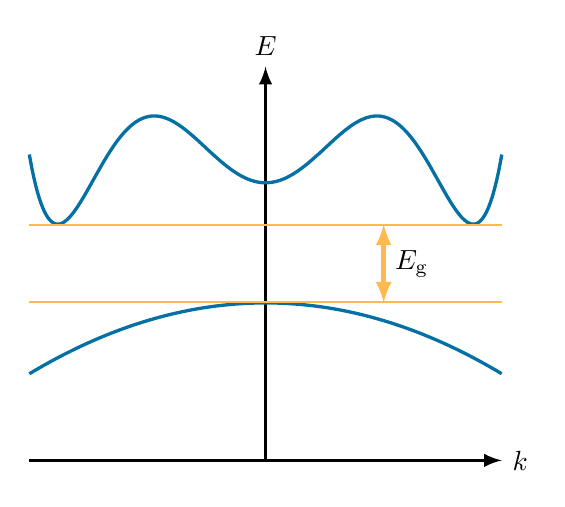
\begin{tikzpicture}
                \draw[very thick, ->] (-3, 0) -- (3, 0) node[right] {\(k\)};
                \draw[very thick, ->] (0, 0) -- (0, 5) node[above] {\(E\)};
                \draw[highlight, very thick, domain=-3:3, samples=100] plot (\x, -0.1*\x*\x+2);
                \draw[highlight, very thick, domain=-3:3, samples=500] plot (\x, {0.01*(1.5*\x-1)*(1.5*\x+1)*(\x-2)*(\x+2)*(\x-3)*(\x+3)+3.885});
                \draw[complementary, ultra thick, <->] (1.5, 2) -- (1.5, 3) node[right, black, midway] {\(E_{\mathrm{g}}\)};
                \draw[complementary, thick] (-3, 2.99) -- (3, 2.99);
                \draw[complementary, thick] (-3, 2.01) -- (3, 2.01);
            \end{tikzpicture}
            \caption{Indirect band gap.}
        \end{subfigure}
        \caption{Direct and indirect band gaps.}
        \label{fig:direct and indirect band gaps}
    \end{figure}
    
    We measure band gaps by measuring the absorbance of light.
    In general if the intensity of light incident on the sample is \(I_{\mathrm{in}}\) and the intensity of the light passes through the sample is \(I_{\mathrm{out}}\) then we define the \defineindex{transmittance} as \(T \coloneqq I_{\mathrm{out}} / I_{\mathrm{in}}\),
    We then define the \defineindex{absorbance} as
    \begin{equation}
        A \coloneqq \log_{10}\left( \frac{I_{\mathrm{in}}}{\mathrm{out}} \right) = \log_{10}\frac{1}{T} = -\log_{10}T.
    \end{equation}
    The absorbance depends on the sample thickness.
    The Beer--Lambert law gives the absorbance as a function of the sample thickness, \(L\):
    \begin{equation}
        I_{\mathrm{out}} = I_{\mathrm{in}} \e^{-\alpha L}
    \end{equation}
    where \(\alpha\) is the \defineindex{absorption coefficient} defined as
    \begin{equation}
        \alpha = \frac{A}{L}\ln 10.
    \end{equation}
    Absorbance, \(A\), is dimensionless and the absorption coefficient, \(\alpha\), has dimensions of inverse length.
    
    The wave vector of optical photons is negligible compared to the wave vector at the Brillouin zone boundary.
    Therefore the wave vector of an electron doesn't change noticeably when a photon is absorbed.
    This means that the electron has to be excited to a state with (approximately) the same wave vector, which means straight upward in the band scheme.
    
    The process for measuring whether a band gap is direct or indirect involves measuring the absorbance for a range of photon frequencies.
    For a direct band gap the absorbance is zero below \(\omega_{\mathrm{g}}\), where \(\omega_{\mathrm{g}}\) is such that \(E_{\mathrm{g}} = \hbar\omega_{\mathrm{g}}\).
    For an indirect band gap on the other hand there will be a small number of absorption processes where a phonon, of frequency \(\Omega\), is annihilated at the same time, donating it's wave vector, and energy, \(\hbar\Omega\), to the electron in addition to the energy, \(\hbar\omega\), donated by the photon.
    This means that a small number of events occur where electrons are excited when \(\omega < \omega_{\mathrm{g}}\).
    This is a relatively rare occurrence due to the need for three particles to interact.
    The resulting shape of a plot of absorbance against photon energy has a characteristic lead in which allows us to distinguish between direct and indirect band gaps.
    See \cref{fig:absorbance}.
    
    \begin{figure}
        \begin{subfigure}{0.4\textwidth}
            \centering
            \tikzsetnextfilename{direct-absorbance}
            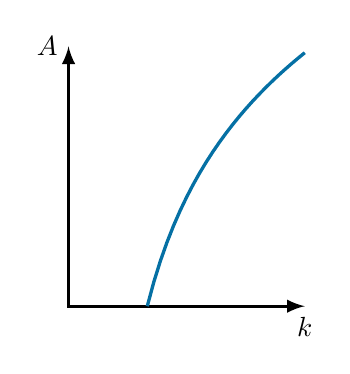
\begin{tikzpicture}
                \draw[very thick, <->] (0, 3.3) node[left] {\(A\)} -- (0, 0) -- (3, 0) node[below] {\(k\)};
                \draw[domain=1:3, highlight, very thick] plot (\x, {2*ln(2*\x - 1)});
            \end{tikzpicture}
            \caption{Direct band gap.}
        \end{subfigure}
        \begin{subfigure}{0.4\textwidth}
            \centering
            \tikzsetnextfilename{indirect-absorbance}
            \begin{tikzpicture}
                \draw[very thick, <->] (0, 3.3) node[left] {\(A\)} -- (0, 0) -- (3, 0) node[below] {\(k\)};
                \draw[domain=1.2:3, highlight, very thick] (0.3, 0) -- plot (\x, {2*ln(2*\x - 1)});
            \end{tikzpicture}
            \caption{Indirect band gap.}
        \end{subfigure}
        \caption{Absorbance of direct and indirect band gaps.}
        \label{fig:absorbance}
    \end{figure}

    \section{Wave Vectors}
    Recall that the group velocity is \(\vv{v_{\mathrm{g}}} = \grad[\vv{k}]\varepsilon(\vv{k})/\hbar\).
    The work done, \(\delta\varepsilon\), in an electric field during a time interval \(\delta t\) is
    \begin{equation}
        \delta\varepsilon = F\delta x = -eE v_{\mathrm{g}}\delta t.
    \end{equation}
    It is also
    \begin{equation}
        \delta \varepsilon = \diff{\varepsilon}{k}\delta k = \hbar v_{\mathrm{g}}\delta k.
    \end{equation}
    Combining these and moving to three dimensions
    \begin{equation}\label{eqn:hbar dk/dt = F}
        \hbar\delta k = -eE\delta t \implies \hbar\diff{\vv{k}}{t} = -e\vv{E} = \vv{F}.
    \end{equation}
    This is the force on an electron in a periodic potential, recall that \(e\) is positive so \(-e\) is the electron charge.
    Putting this in the Lorentz force equation we have
    \begin{equation}
        \vv{F} = \hbar\diff{\vv{k}}{t} = -e(\vv{E} + \vv{v} \times \vv{B}) = -e(\vv{E} + \frac{1}{\hbar}\grad[\vv{k}]\varepsilon \times\vv{B}).
    \end{equation}
    
    \section{Holes}
    Consider what happens when an electron is excited from the valence band to the conduction band.
    Suppose we start with \(10^{20}\) electrons.
    We can then describe the properties of the valence band in terms of the \(10^{20} - 1\) populated valence band states.
    Alternatively, we can describe them in terms of the one vacant state.
    Clearly this is much easier to do.
    We treat the vacant state as a quasiparticle, which we call a \defineindex{hole}.
    
    With no excited electrons the total wave vector of the filled valence band is \(\vv{0}\).
    Removing an electron with wave vector \(\vv{k_{\mathrm{e}}}\) means that the total wave vector of the remaining electrons in the valence band is \(-\vv{k_{\mathrm{e}}}\).
    We can identify this as the wave vector of the hole, \(\vv{k_{\mathrm{h}}} = -\vv{k_{\mathrm{e}}}\).
    
    Similarly the energy of the hole state is the missing energy of the removed electron, that is \(\varepsilon_{\mathrm{h}}(\vv{k_{\mathrm{h}}}) = -\varepsilon_{\mathrm{e}}(\vv{k_{\mathrm{e}}})\).
    
    At zero kelvin we can place the Fermi energy, that is the highest point in the valence band, at zero.
    We then get that the flipped valence band gives the properties of the hole.
    See \cref{fig:hole band}.
    
    \begin{figure}
        \tikzsetnextfilename{hole-band}
        \begin{tikzpicture}
            \draw[very thick, ->] (-3, 0) -- (3, 0) node[right] {\(k\)};
            \draw[very thick, ->] (0, -3) -- (0, 3) node[above] {\(\varepsilon\)};
            \draw[highlight, very thick, domain=-3:3, samples=100] plot (\x, -\x*\x/3);
            \draw[complementary, very thick, domain=-3:3, samples=100] plot (\x, \x*\x/3);
            \draw (-2, -4/3) -- (2, 4/3);
            \draw[highlight] (-2, -4/3) -- (-2, 0);
            \node[above, highlight] at (-1.9, 0) {\(k_{\mathrm{e}}\)};
            \draw[complementary] (2, 4/3) -- (2, 0);
            \node[below, complementary] at (2.1, 0) {\(k_{\mathrm{h}}\)};
            \draw[highlight, fill=white, thick] (-2, -4/3) circle [radius = 0.075cm];
            \draw[complementary, fill=complementary] (2, 4/3) circle [radius = 0.075cm];
        \end{tikzpicture}
        \caption[Hole band.]{The hole band is constructed by setting \(\vv{k_{\mathrm{h}}} = \vv{k_{\mathrm{e}}}\) and \(\varepsilon_{\mathrm{h}}(\vv{k_{\mathrm{h}}}) = -\varepsilon_{\mathrm{e}}(\vv{k_{\mathrm{e}}})\).}
        \label{fig:hole band}
    \end{figure}

    To find the group velocity of the hole we can simply use the hole wave vector and dispersion relation, the identity \(\grad[-\vv{k}] f(\vv{k}) = -\grad[\vv{k}]f(\vv{k})\), and the fact that, for non-magnetic materials, the dispersion relations are symmetric under inversion so \(\varepsilon_{\mathrm{e}}(-\vv{k_{\mathrm{e}}}) = \varepsilon_{\mathrm{e}}(-\vv{k_{\mathrm{e}}})\):
    \begin{equation}
        \vv{v_{\mathrm{h}}}(\vv{k_{\mathrm{h}}}) = \grad[\vv{k_{\mathrm{h}}}] \varepsilon_{\mathrm{h}}(\vv{k_{\mathrm{h}}}) = \grad[-\vv{k_{\mathrm{e}}}](-\varepsilon(\vv{-k_{\mathrm{e}}})) = \grad[\vv{k_{\mathrm{e}}}]\varepsilon(\vv{-k_{\mathrm{e}}}) = \grad[\vv{k_{\mathrm{e}}}]\varepsilon(\vv{k_{\mathrm{e}}}) = \vv{v_{\mathrm{e}}}(\vv{k_{\mathrm{e}}}).
    \end{equation}
    So the velocity of the hole is the same as the velocity of the electron.
    
    We will introduce the concept of effective mass, \(m^*\), in a later section. % TODO: Add link to section where effective mass is introduced
    For now we just talk of the mass and make a note here that what we are actually considering is the effective mass.
    Analogously to the hole wave vector and energy being the negative of the electrons since the represent \enquote{missing} quantities the hole mass is \(m_{\mathrm{h}} = -m_{\mathrm{e}}\).
    
    The charge of the hole is the missing charge of the removed electron, so \(q_{\mathrm{h}} = -q_{\mathrm{e}}\).
    
    The equation of motion for the hole is then
    \begin{equation}
        \hbar \diff{\vv{k_{\mathrm{h}}}}{t} = e(E + \vv{v_{\mathrm{h}}} \times \vv{B}).
    \end{equation}
    Since \(\vv{v_{\mathrm{h}}} = \vv{v_{\mathrm{e}}}\) the only difference here is that for an electron there is an extra overall negative due to the charge.
    So we see that a hole behaves like a quasiparticle with positive charge, \(e\).
    
    Now consider what happens when we apply an electric field, say in the positive \(x\)-direction (by which we really mean the direction \((1, 0, 0)\) in reciprocal space).
    As long as there is no scattering the electrons, which are negative, are all accelerated in the negative \(x\)-direction.
    The state where there is a hole is filled in by the electron to its right and the hole therefore moves right, in the positive \(x\)-direction.
    The electron in the state at the left edge of the Brillouin zone, \(k = -\pi/a\), moves to the equivalent state \(k' = k + 2\pi/a\).
    
    The hole moves in the opposite direction to the electrons and has opposite charge.
    Therefore the current is \(\vv{j} = (-e)\vv{v_{\mathrm{hole}}} = e\vv{v_{\mathrm{electron}}}\).
    Note that the velocities here have \emph{opposite signs} since we are considering the motion of a hole and a different electron.
    Before, when we concluded that the electron and hole velocities are equal, we were considering the hole and the electron that was removed to create it.
    So the current due to motion of an electron is the same as the current due to the motion of the hole.
    This means that we can describe the current from the nearly filled valence band in terms of either holes or electrons.
    
    \begin{table}
        \caption{Summary of hole properties.}
        \begin{tabular}{lcc}\toprule
            Quantity & Electron & Hole\\\midrule
            Wave Vector & \(\vv{k_{\mathrm{e}}}\) & \(\vv{k_{\mathrm{h}}} = -\vv{k_{\mathrm{e}}}\)\\
            Energy & \(\varepsilon_{\mathrm{e}}(\vv{k_{\mathrm{e}}})\) & \(\varepsilon_{\mathrm{h}}(\vv{k_{\mathrm{h}}})=-\varepsilon_{\mathrm{e}}(\vv{k_{\mathrm{e}}})\)\\
            Velocity & \(\vv{v_{\mathrm{e}}}\) & \(\vv{v_{\mathrm{h}}} = - \vv{v_{\mathrm{e}}}\)\\
            Effective Mass & \(m_{\mathrm{e}}^*\) & \(m_{\mathrm{h}}^* = - m_{\mathrm{e}}^*\)\\
            Charge & \(q_{\mathrm{e}}\) & \(q_{\mathrm{h}} = -q_{\mathrm{e}}\)\\
            Current & \(\vv{j}\) & \(\vv{j}\)\\\bottomrule
        \end{tabular}
    \end{table}
    
    One place where the distinction between electrons and holes is important is the Hall effect.
    When we calculate the Hall coefficient for holes we will get the \emph{negative} of the Hall coefficient for electrons.
    Since the Hall coefficient for electrons is negative this results in a positive Hall coefficient for holes.
    We can use this to measure whether holes or electrons dominate current flow.
    For example, beryllium is a semimetal with one nearly full band and one mostly empty band.
    The Hall effect from electrons and holes almost cancels but not quite and the resulting Hall coefficient is positive as the holes contribute slightly more to the current.
    
    \section{Effective Mass}
    For the free electron dispersion relation,
    \begin{equation}
        \varepsilon(k) = \frac{\hbar^2}{2m}
    \end{equation}
    the curvature of the band is determined, as usual, by the second derivative, which in this quadratic case is simply proportional to the coefficient, \(\hbar^2/(2m)\).
    We see, therefore, that the band curvature depends on the electron mass.
    In this section we ask whether this relation is reversible, can we find the electron mass from the curvature?
    We can't, but we can find a quantity with dimensions of mass that has physical meaning.
    
    Recall that we found
    \begin{equation}
        \hbar\diff{k}{t} = F
    \end{equation}
    earlier in \cref{eqn:hbar dk/dt = F}, and that the group velocity is defined as
    \begin{equation}
        v_{\mathrm{g}} = \frac{1}{\hbar} \diff{\varepsilon}{k}.
    \end{equation}
    The acceleration is then
    \begin{equation}
        \diff{v_{\mathrm{g}}}{t} = \frac{1}{\hbar} \diff*{\diff{\varepsilon}{k}}{t} = \frac{1}{\hbar} \diff[2]{\varepsilon}{k}\diff{k}{t} = \frac{1}{\hbar^2}\diff[2]{\varepsilon}{k}F.
    \end{equation}
    Rearranging this we have
    \begin{equation}
        F = \hbar^2\left( \diff[2]{\varepsilon}{k} \right)^{-1} \diff{v_{\mathrm{g}}}{t} = m^*\diff{v_{\mathrm{g}}}{t}.
    \end{equation}
    Here we have defined the \defineindex{effective mass}
    \begin{equation}
        m^* \coloneqq \hbar^2\left( \diff[2]{\varepsilon}{k} \right)^{-1}.
    \end{equation}
    That is the effective mass is defined to be inversely proportional to the band curvature.
    
    This definition of the effective mass coincides with the electron mass in the free electron case.
    In reality the effective mass and electron mass will be different.
    We can think of the effective mass as the electron mass corrected for the potential.
    It should be noticed that the effective mass can be negative.
    This corresponds to an electron being back scattered, being accelerated in the opposite direction to what one would expect for a free electron.
    Replacing the electron mass with the effective mass in many of our previous results will give a more accurate value.
    
    \subsection{In Three Dimensions}
    In three dimensions the curvature is, in general, a tensor quantity.
    Generalising the definition of the effective mass we define the \define{effective mass tensor}\index{effective mass!tensor},
    \begin{equation}
        \left( \frac{1}{m^*} \right)_{ij} \coloneqq \frac{1}{\hbar^2} \diff*{\diff{\varepsilon}{k_j}}{k_i}.
    \end{equation}
    This relates to the acceleration by
    \begin{equation}
        \diff{v_i}{t} = \sum_{j=1}^{3} \left( \frac{1}{m^*} \right)_{ij}F_j.
    \end{equation}
    
    \section{Typical Semiconductor Band Structures}
    \subsection{Silicon}
    Silicon has a diamond like structure, that means an FCC lattice, but not an FCC structure.
    It has an indirect band gap of \(E_{\mathrm{g}} = \qty{1.17}{\electronvolt}\) at \qty{0}{\kelvin}, and \(E_{\mathrm{g}} = \qty{1.12}{\electronvolt}\) at \qty{300}{\kelvin}.
    Both much larger than the energy, \(\boltzmann T \approx \qty{25}{\milli\electronvolt}\), available at room temperature.
    The lowest band is nearly parabolic and has a minimum at the \(\Gamma\) point (\(\vv{k} = \vv{0}\)).
    This is pretty much what we would expect from the free electron approximation.
    The maximum of the valence band also occurs near the \(\Gamma\) point.
    The minimum of the conduction band occurs near the \(X\) point, which makes the band gap indirect.
    
    \subsection{Germanium}
    Germanium has the diamond structure, similar to silicon.
    It has a similar band structure also.
    The band gap is smaller, \(E_{\mathrm{g}} = \qty{0.75}{\electronvolt}\) at \qty{0}{\kelvin}, or \(E_{\mathrm{g}} = \qty{0.67}{\electronvolt}\) at \qty{300}{\kelvin}.
    The lowest band and valence band both have extrema at the \(\Gamma\) point, like silicon.
    The minimum of the conduction band is at the \(L\) point.
    This is an indirect band gap.
    Spin-orbit coupling lifts degeneracies and creates band splitting compared to silicon.
    
    \subsection{Gallium Arsenide}
    Gallium Arsenide has the zinc blende structure, which is the diamond structure but with two types of atom.
    It has a direct band gap at the \(\Gamma\) point.
    The band gap is \(E_{\mathrm{g}} = \qty{1.52}{\electronvolt}\) at \qty{0}{\kelvin}, and \(E_{\mathrm{g}} = \qty{1.43}{\electronvolt}\) at \qty{300}{\kelvin}.
    
    \section{Intrinsic Semiconductors}
    Semiconductors are characterised by having electrical conductivity at room temperature which is several orders of magnitude lower than a metal, but not zero like a conductor.
    The electrical conductivity increases exponentially with temperature.
    It is this property that we will now look at, starting with intrinsic semiconductors.
    An \defineindex{intrinsic semiconductor} is a perfect semiconductor without structural defects or chemical impurities.
    This means no doping.
    Clearly intrinsic semiconductors don't exist in real life but there are many materials that are reasonably close.
    
    Current is carried by free charge carriers.
    In a semiconductor each excited electron gives \emph{two} free charge carriers, the electron itself and the hole.
    Most of the excited electrons are thermally excited, but some will also be excited by absorption of a photon.
    At \qty{0}{\kelvin} we expect that an intrinsic semiconductor will have zero conductivity.
    
    We can express the conductivity, \(\sigma\), in terms of the electron and hole concentrations, \(n\) and \(p\) respectively (for negative and positive), as well as the electron and hole mobilities, \(\mu_n\) and \(\mu_p\).
    The charge carrier \defineindex{mobility}, \(\mu\), is a quantity relating the carrier drift velocity, \(v_{\mathrm{d}}\), to the electric field, \(v_{\mathrm{d}} = \mu E\).
    For a free electron Fermi gas model the mobility is \(\mu = e\tau/m^*\), where \(\tau\) si the average time between scattering events, \(e\) is the elementary charge, and \(m^*\) is the effective mass.
    In this context we often call the free electron Fermi gas model the \defineindex{Drude--Sommerfeld model}.
    
    \subsection{Conductivity}
    With the starting point of the free electron gas model the conductivity is
    \begin{equation}
        \sigma = \frac{ne^2\tau}{m^*}.
    \end{equation}
    Including holes and writing this in terms of the mobility the conductivity is
    \begin{equation}
        \sigma = \abs{e} (n\mu_n + p\mu_p).
    \end{equation}
    Note that both electrons and holes contribute with the same sign, since the current for holes is the same as the current for electrons in the same magnetic field as the direction of travel and charge are both reversed, cancelling out.
    
    The temperature dependence comes from the temperature dependence of \(n\) and \(p\).
    In order to predict this we model the valence and conduction bands as one parabolic band each, more accurate band structures don't yield analytic results and we have to resort to numerical methods.
    We then make use of results from the free electron gas model, in particular the density of states.
    
    Annoyingly there are two different ways that the density of states is defined.
    So far we have been using \(D(\varepsilon)\) taking
    \begin{equation}
        \int_{0}^{\infty} D(\varepsilon)f(\varepsilon, T) \dd{\varepsilon}
    \end{equation}
    to give the number of electrons.
    In this section we will use the density of states, \(\tilde{D}(\varepsilon)\), such that
    \begin{equation}
        \int_{0}^{\infty} \tilde{D}(\varepsilon) f(\varepsilon, T) \dd{\varepsilon}
    \end{equation}
    gives the \emph{density} of electrons.
    So \(\tilde{D} = D/V\).
    Both \(D\) and \(\tilde{D}\) are usually denoted \(D\) and it is left to context to determine which is being used.
    It is this second type, \(\tilde{D}\), which we make use of in this section, and following conventions, we denote it \(D\) from here on.
    
    The electron concentration is
    \begin{equation}
        n = \int_{\varepsilon_{\mathrm{c}}}^{\infty} D_{\mathrm{c}}(\varepsilon) f(\varepsilon, T) \dd{\varepsilon}
    \end{equation}
    where \(\varepsilon_{\mathrm{c}}\) is the minimum energy in the conduction band.
    For the conduction band the density of states is
    \begin{equation}
        D_{\mathrm{c}}(\varepsilon) = \frac{(2m_n^*)^{3/2}}{2\pi^2\hbar^3}\sqrt{\varepsilon - \varepsilon_{\mathrm{c}}}, \qquad\text{for \(\varepsilon > \varepsilon_{\mathrm{c}}\)}.
    \end{equation}
    At normal temperatures, such that \(\boltzmann T \ll \varepsilon - \varepsilon_{\fermi}\), we can approximate the Fermi--Dirac distribution using the fact that \(\e^{\beta(\varepsilon - \varepsilon_{\fermi})}\) will be small:
    \begin{equation}
        f(\varepsilon) - \frac{1}{\varepsilon^{\beta(\varepsilon - \varepsilon_{\fermi})} + 1} \approx \e^{-\beta(\varepsilon - \varepsilon_{\fermi})} = \e^{\beta\varepsilon_{\fermi}}\e^{-\beta \varepsilon}.
    \end{equation}
    
    We then have
    \begin{align}
        n &= \int_{\varepsilon_{\mathrm{c}}}^{\infty} D_{\mathrm{c}}(\varepsilon)f(\varepsilon, T) \dd{\varepsilon}\\
        &\approx \frac{(2m_n^*)^{3.2}}{2\pi^2\hbar^3} \e^{\beta\varepsilon_{\fermi}} \int_{\varepsilon_{\mathrm{c}}}^{\infty} \e^{-\beta\varepsilon}\sqrt{\varepsilon - \varepsilon_{\mathrm{c}}} \dd{\varepsilon}.
    \end{align}
    Considering this integral, defining \(x = \beta(\varepsilon - \varepsilon_{\mathrm{c}})\) we have
    \begin{align}
        n &\approx \frac{(2m_n^*)^{3/2}}{2\pi^2\hbar^3}(\boltzmann T)^{3/2} \e^{-\beta(\varepsilon_{\mathrm{c}} - \varepsilon_{\fermi})} \int_{0}^{\infty} x^{1/2} \e^{-x}\dd{x}\\
        &= \frac{(2m_n^*)^{3/2}}{2\pi^2\hbar^3}(\boltzmann T)^{3/2} \e^{-\beta(\varepsilon_{\mathrm{c}} - \varepsilon_{\fermi})} \Gamma\left( \frac{3}{2} \right)\\
        &= \frac{(2m_n^*)^{3/2}}{2\pi^2\hbar^3}(\boltzmann T)^{3/2} \e^{-\beta(\varepsilon_{\mathrm{c}} - \varepsilon_{\fermi})} \frac{\sqrt{\pi}}{2}
    \end{align}
    where we have recognised the gamma function
    \begin{equation}
        \Gamma(z+1) \coloneqq \int_{0}^{\infty} \int_{0}^{\infty} x^{z}\e^{-x} \dd{x}, \qqand \Gamma\left( \frac{3}{2} \right) = \frac{\sqrt{\pi}}{2}.
    \end{equation}
    This gives us the final result
    \begin{equation}
        n(T) = 2\left( \frac{m_n^*\boltzmann T}{2\pi\hbar^2} \right)^{3/2} \e^{-\beta(\varepsilon_{\mathrm{c}} - \varepsilon_{\mathrm{F}})}.
    \end{equation}
    
    We can make an analogous computation for the holes in the valence band, the only difference being we are now considering hole energies below the Fermi level so \(-(\varepsilon_{\mathrm{c}} - \varepsilon_{\fermi}) \to -(\varepsilon_{\fermi} - \varepsilon_{\mathrm{v}}) = \varepsilon_{\mathrm{v}} - e_{\fermi}\).
    The hole density is then
    \begin{equation}
        p(T) = 2\left( \frac{m_p^*\boltzmann T}{2\pi\hbar^2} \right)^{3/2} \e^{\beta(\varepsilon_{\mathrm{v}} - \varepsilon_{\fermi})}.
    \end{equation}
    
    In an intrinsic semiconductor every free electron has a corresponding free hole.
    Therefore the number of electrons and holes, and hence their concentrations, are the same.
    We can use this to eliminate the unknown Fermi level, \(\varepsilon_{\fermi}\).
    We also add subscript \(\mathrm{i}\) to denote that this only applies to intrinsic semiconductors.
    Doing so we have
    \begin{equation}
        n_{\mathrm{i}} = p_{\mathrm{i}} = 2 \left( \frac{\boltzmann T}{2\pi \hbar^2} \right)^{3/2} (m_n^*m_p^*)^{3/2} \e^{-E_{\mathrm{g}}\beta/2}.
    \end{equation}
    Here we have identified \(\varepsilon_{\mathrm{c}} - \varepsilon_{\mathrm{v}} = E_{\mathrm{g}}\).
    
    From this we see that the temperature dependence is mostly from the \(\e^{-E_{\mathrm{g}}/(2\boltzmann T)}\) term.
    There is also a small correction from the \(T^{3/2}\) term.
    As well as the temperature dependence here the electron and hole mobilities are also temperature dependent, although this effect is much smaller than the exponential dependence in \(n_{\mathrm{i}}\) and \(p_{\mathrm{i}}\).
    This matches experimental data quite well if we choose the effective masses \(m_n^*\) and \(m_p^*\) as parameters to our model.
    To get a sense of size of these quantities see \cref{tab:electron concentration}.
    
    \begin{table}
        \caption[Typical band gaps and electron concentrations.]{Typical band gaps and free electron concentrations for some intrinsic semiconductors and the free electron concentrations of some metals for comparison.}
        \label{tab:electron concentration}
        \begin{tabular}{lll}\toprule
            Material & \(E_{\mathrm{g}}/\unit{\electronvolt}\) & \(n_{\mathrm{i}}/\unit{\per\centi\metre\cubed}\)\\\midrule
            \ce{Ge} & 0.67 & \(2.4 \times 10^{13}\)\\
            \ce{Si} & 1.1 & \(1.5 \times 10^{10}\)\\
            \ce{GaAs} & 1.43 & \(5.0 \times 10^{7}\)\\
            \ce{Na} & N/A & \(2.7 \times 10^{22}\)\\
            \ce{Al} & N/A & \(18 \times 10^{22}\)\\\bottomrule
        \end{tabular}
    \end{table}
    
    \section{Temperature Dependence of the Fermi Level}
    An intrinsic neutral semiconductor must be charge neutral at all temperatures.
    This means that \(n_{\mathrm{i}}(T) = p_{\mathrm{i}}(T)\).
    The density of occupied conduction band states is given by
    \begin{equation}
        \diff{n}{\varepsilon} = D_{\mathrm{c}}(\varepsilon) f(\varepsilon, \varepsilon_{\fermi}, T).
    \end{equation}
    For the valence band holes we need to consider the missing electrons, so we replace \(f(\varepsilon, \varepsilon_{\fermi}, T)\) with \(1 - \varphi(\varepsilon, \varepsilon_{\fermi}, T)\).
    Integrating the occupied densities of states over the relevant energy ranges for the conduction and valence band we we get the electron and hole concentrations.
    That is the concentrations are given by the area under the \(\diff{n}/{\varepsilon}\) and \(\diff{p}/{\varepsilon}\) curves.
    
    Consider the case of \(m_p^* = 2m_n^*\), and \(\varepsilon_{\fermi}\) is directly between \(\varepsilon_{\mathrm{v}}\) and \(\varepsilon_{\mathrm{c}}\).
    In this case \(p_{\mathrm{i}}\) will be larger than \(n_{\mathrm{i}}\).
    Since this can't be true we see that the Fermi level must be at a different point.
    Shifting it up slightly we will find a value such that \(n_{\mathrm{i}} = p_{\mathrm{i}}\).
    
    In general by comparing the densities we have
    \begin{align}
        n_{\mathrm{i}}(T) &= p_{\mathrm{i}}(T)\\
        (m_n^*)^{3/2}\e^{-\beta(\varepsilon_{\mathrm{c} - \varepsilon_{\fermi}})} &= (m_p^*)^{3/2}\e^{\beta(\varepsilon_{\mathrm{v}} - \varepsilon_{\fermi})}\\
        \frac{\e^{-\beta(\varepsilon_{\mathrm{c}} - \varepsilon_{\fermi})}}{\e^{\beta(\varepsilon_{\mathrm{v}} - \varepsilon_{\fermi})}} &= \frac{(m_p^*)^{3/2}}{(m_n^*)^{3/2}}\\
        [(\varepsilon_{\fermi} - \varepsilon_{\mathrm{c}}) - (\varepsilon_{\mathrm{v}} - \varepsilon_{\fermi})] &= \frac{3}{2}\boltzmann T\ln\left( \frac{m_p^*}{m_n^*} \right)\\
        \varepsilon_{\fermi} = \frac{1}{2}(\varepsilon_{\mathrm{c}} + \varepsilon_{\mathrm{v}}) + \frac{3}{4}\boltzmann T\ln\left( \frac{m_p^*}{m_n^*} \right).
    \end{align}
    This shows that at \qty{0}{\kelvin} the Fermi level is in the middle of the band gap and then at higher temperatures shifts by an amount proportional to \(\boltzmann T\).
    The sign of the shift depends on the ratio of the effective masses.
    The value of \(\varepsilon_{\fermi}\) depends on the density of states, through \(m_n^*\) and \(m_p^*\).
    
    For example, consider silicon.
    The band gap is \(E_{\mathrm{g}} = \qty{1.1}{\electronvolt}\) at \(\qty{300}{\kelvin}\).
    The electron mass is \(m_n^* = \qty{1.1}{\electronmass}\), and the hole mass is \(m_p^* = \qty{0.7}{\electronmass}\).
    At temperature \(T\) the shift from the \qty{0}{\kelvin} value of \(\varepsilon_{\fermi}\) is
    \begin{equation}
        \frac{3}{4}\boltzmann T \ln\left( \frac{0.7}{1.1} \right) \approx -0.45\boltzmann T.
    \end{equation}
    For example when going from \qty{0}{\kelvin} to \qty{300}{\kelvin} the Fermi level shifts by approximately \(-0.45\cdot \qty{25}{\milli\electronvolt} \approx \qty{-11}{\milli\electronvolt}\).
    In general the shift in Fermi level will be small compared to the size of the band gap.
    
    \section{Doping}
    In a real material we cannot avoid impurities.
    These can greatly change the properties of the material.
    For example, a high purity sample of \ce{GaAs} has a carrier concentration of approximately \(10^{16}\,\unit{\per\centi\metre\cubed}\).
    On the other hand for a truly pure sample we expect the intrinsic density to be approximately \(\qty{5e7}{\per\centi\metre\cubed}\).
    Another example is silicon, which has an intrinsic carrier concentration of approximately \(\qty{1.5e10}{\per\centi\metre\cubed}\).
    This is not large enough to be useful in semiconductor devices.
    
    We modify carrier charge density by intentionally introducing chemical impurities, a process called \defineindex{doping}.
    Typically there are two types of doping materials.
    Donors give electrons to the crystal and trap holes, this increases \(n\) and decreases \(p\).
    We call the resulting material \(n\)-type.
    Acceptors trap electrons and release holes, this increases \(p\) and decreases \(n\).
    We call the resulting material \(p\)-type.
    
    Donors have more valence electrons than are needed for bonding in the material being doped, and acceptors have fewer.
    For example \ce{Si} and \ce{Ge} are tetravalent, that is each atom forms four bonds.
    In this context \ce{P}, \ce{As}, and \ce{Sb} are donors as they are pentavalent, so adding some of these adds an equal amount of weakly electrons.
    \ce{B}, \ce{Al}, \ce{Ga}, and \ce{In} are trivalent, and so acceptors in this context.
    Adding some of these adds weakly bound holes.
    
    \section{Charge Carrier Density}
    Recall that the charge carrier densities are
    \begin{align}
        n(T) &= 2\left( \frac{m_n^*\boltzmann T}{2\pi\hbar^2} \right)^{3/2} \e^{-\beta(\varepsilon_{\mathrm{c}} - \varepsilon_{\fermi})},
        p(T) &= 2\left( \frac{m_p^*\boltzmann T}{2\pi\hbar^2} \right)^{3/2} \e^{\beta(\varepsilon_{\mathrm{v}} - \varepsilon_{\fermi})}.
    \end{align}
    The derivation up to this point works for doped and intrinsic semiconductors.
    The analysis breaks down when we set \(n_{\mathrm{i}} = p_{\mathrm{i}}\), which holds only for intrinsic semiconductors.
    The assumptions made to derive this model was that the bands are approximately parabolic and that \(\varepsilon_{\mathrm{c}} - \varepsilon_{\fermi}, \varepsilon_{\fermi} - \varepsilon_{\mathrm{v}} \gg \boltzmann T\).
    Consider the product
    \begin{equation}
        np = 4\left( \frac{\boltzmann T}{2\pi\hbar^2} \right)^{3} (m_n^*m_p^*)^{3/2} \e^{-\beta E_{\mathrm{g}}}.
    \end{equation}
    This is the same result as we had for \(n_{\mathrm{i}}p_{\mathrm{i}}\), the only thing that changes between an intrinsic semiconductor and a doped semiconductor is the balance of electrons and holes.
    In an intrinsic semiconductor we have equal amounts of both whereas in a doped semiconductor we won't, but their product will be the same.
    This is known as the \defineindex{law of mass action}.
    
    \section{Impurity as Hydrogen Like Centre}
    We will consider here a donor impurity but the analysis applies to acceptor impurities also.
    The donor atom will have some excess positive charge, compared to the cores of the other atoms in the material.
    The weakly bound electron can be treated like the electron in a Hydrogen atom, with a different nuclear charge.
    In particular recall that the Rydberg energy levels are given by
    \begin{equation}
        E_n^{\ce{H}} = \frac{m_{\mathrm{e}} e^4}{2(4\pi\varepsilon_0\hbar)^2} \frac{1}{n^2}.
    \end{equation}
    For the impurity we replace \(m_{\mathrm{e}}\) with \(m_n^*\), and \(\varepsilon_{0}\) with \(\varepsilon_{0}\varepsilon\), where \(\varepsilon\) is the dielectric constant for the crystal.
    We then have
    \begin{equation}
        E_n^{\mathrm{donor}} = \frac{m_n^*e^4}{2(4\pi\varepsilon_0\varepsilon\hbar)^2}\frac{1}{n^2} = \frac{m_n^*/m_{\mathrm{e}}}{\varepsilon^2}E_n^{\ce{H}}.
    \end{equation}
    
    For example, in silicon \(m_n^* \approx \qty{0.3}{\electronmass}\), \(\varepsilon \approx 11.7\), so
    \begin{equation}
        \frac{m_n^*/m_{\mathrm{e}}}{\varepsilon^2} \approx 0.0022.
    \end{equation}
    Therefore, recalling that \(E_1^{\ce{H}} = \qty{13.6}{\electronvolt}\), the ground state binding energy for donor doping in silicon is
    \begin{equation}
        E_1^{\mathrm{donor}} \approx 0.0022 \cdot \qty{13.6}{\electronvolt} \approx \qty{30}{\milli\electronvolt}.
    \end{equation}
    We see that the donor electrons are only weakly bound compared to the band gap, which is about \qty{1.1}{\electronvolt} for silicon.
    This means that the donor electron is easily liberated to become a charge carrier, which is exactly what we want.
    In particular at room temperature \(\boltzmann T \approx \qty{25}{\milli\electronvolt}\) so a lot of donor electrons will be released purely by thermal fluctuations.
    
    We can define a quantity analogous to the Bohr radius in hydrogen:
    \begin{equation}
        r = \varepsilon_0\varepsilon \frac{h^2}{\pi m_n^*e^2} = \varepsilon\frac{m_{\mathrm{e}}}{m_n^*}a_0.
    \end{equation}
    This can be thought of as a measure of how tightly bound the electron is to the donor atom.
    Going back to the donor doped silicon example we have that \(r \approx (11.7/0.3) a_0 \approx \qty{20}{\angstrom}\).
    In a standard silicon crystal the interatomic distance is \qty{2.35}{\angstrom}.
    From this we see that the donor electron cloud, which we take to be the volume enclosed by a sphere of radius \(r\) centred on the donor atom, extends over approximately 1000 silicon atoms.
    This justifies the need for the factor of \(\varepsilon\) since the donor electron is screened from the donor nucleus by many silicon atoms, which we account for with this factor of \(\varepsilon\).
    
    Further verification of this model is provided by accurately predicting absorbance patterns.
    
    For an acceptor impurity instead of energy levels just below the valence band the hole has energy levels just above the conduction band.
    
    \section{Semiconductor Devices}
    A semiconductor device is usually formed by placing some \(p\)-type material next to some \(n\)-type material.
    This produces an interface, known as a \(p\)-\(n\) junction.
    Bringing these two materials together we get a boundary region where the energy levels and bands move smoothly from one to the other.
    The Fermi level is the same for the entire crystal, including across the junction.
    See \cref{fig:pn junction}.
    Depending on the desired result we can then apply a current to this either from \(p\) to \(n\) or \(n\) to \(p\).
    If we do so one way then we will add electrons to the \(n\)-type increasing the difference between the two sides of the junction and allowing current flow.
    If we do so the other way no current can pass, this is the basics of how a diode is formed.
    
    Many other devices can be formed in a similar way, such as transistors, the simplest of which have \(npn\) junctions and \(pnp\) junctions.
    Construction of semiconductor devices is a whole course to itself so we shall stop here.
    
    \begin{figure}
        \begin{subfigure}{0.8\textwidth}
            \centering
            \tikzsetnextfilename{p-and-n-energy-levels}
            \begin{tikzpicture}
                \draw[very thick, ->] (-0.6, 0) -- (-0.6, 4) node[left] {\(E\)};
                \fill[highlight!20] (0, 1) rectangle (3, 0);
                \draw[highlight, thick] (0, 1) -- (3, 1);
                \node[below right, highlight, font=\tiny] at (0, 1) {Valence Band};
                \node[left, font=\tiny] at (0, 1) {\(E_{\mathrm{v}}\)};
                \draw[highlight, thick] (0, 1.3) -- (3, 1.3);
                \node[left, font=\tiny] at (0, 1.3) {\(E_{\mathrm{a}}\)};
                \draw[highlight, thick] (0, 1.6) -- (3, 1.6);
                \node[left, font=\tiny] at (0, 1.6) {\(\varepsilon_{\mathrm{F}}\)};
                \fill[highlight!20] (0, 3) rectangle (3, 4);
                \node[above right, font=\tiny, highlight] at (0, 3) {Conduction Band};
                \draw[highlight, thick] (0, 3) -- (3, 3);
                \node[left, font=\tiny] at (0, 3) {\(E_{\mathrm{c}}\)};
                
                \fill[highlight!20] (5, 1) rectangle (8, 0);
                \draw[highlight, thick] (5, 1) -- (8, 1);
                \node[below right, highlight, font=\tiny] at (5, 1) {Valence Band};
                \node[right, font=\tiny] at (8, 1) {\(E_{\mathrm{v}}\)};
                \draw[highlight, thick] (5, 2.7) -- (8, 2.7);
                \node[right, font=\tiny] at (8, 2.7) {\(E_{\mathrm{d}}\)};
                \draw[highlight, thick] (5, 2.4) -- (8, 2.4);
                \node[right, font=\tiny] at (8, 2.4) {\(\varepsilon_{\mathrm{F}}\)};
                \fill[highlight!20] (5, 3) rectangle (8, 4);
                \node[above right, font=\tiny, highlight] at (5, 3) {Conduction Band};
                \draw[highlight, thick] (5, 3) -- (8, 3);
                \node[right, font=\tiny] at (8, 3) {\(E_{\mathrm{c}}\)};
                \node[above] at (1.5, 4) {\(p\)-type};
                \node[above] at (6.5, 4) {\(n\)-type};
                \draw[gray] (4, -0.2) -- (4, 4.5);
            \end{tikzpicture}
            \caption{The bands and energy levels of the doped electrons in \(p\) and \(n\)-type semiconductors.}
        \end{subfigure}
        \begin{subfigure}{0.8\textwidth}
            \centering
            \tikzsetnextfilename{pn-junction}
            \begin{tikzpicture}
                \draw[very thick, ->] (-0.6, -0.8) -- (-0.6, 4) node[left] {\(E\)};
                \fill[highlight!20] (0, -0.8) -- (0, 1) -- (3, 1) to[out=0, in=180] (5, 0.2) -- (8, 0.2) -- (8, -0.8) -- cycle;
                \draw[highlight, thick] (0, 1) -- (3, 1);
                \node[below right, highlight, font=\tiny] at (0, 1) {Valence Band};
                \node[left, font=\tiny] at (0, 1) {\(E_{\mathrm{v}}\)};
                \draw[highlight, thick] (0, 1.3) -- (3, 1.3);
                \node[left, font=\tiny] at (0, 1.3) {\(E_{\mathrm{a}}\)};
                \draw[highlight, thick] (0, 1.6) -- (8, 1.6);
                \node[left, font=\tiny] at (0, 1.6) {\(\varepsilon_{\mathrm{F}}\)};
                \fill[highlight!20] (0, 3) -- (3, 3) to[out=0, in=180] (5, 2.2) -- (8, 2.2) -- (8, 4) -- (0, 4) -- cycle;
                \node[above right, font=\tiny, highlight] at (0, 3) {Conduction Band};
                \draw[highlight, thick] (0, 3) -- (3, 3);
                \node[left, font=\tiny] at (0, 3) {\(E_{\mathrm{c}}\)};
                
                \draw[highlight, thick] (5, 0.2) -- (8, 0.2);
                \node[right, font=\tiny] at (8, 0.2) {\(E_{\mathrm{v}}\)};
                \draw[highlight, thick] (5, 1.9) -- (8, 1.9);
                \node[right, font=\tiny] at (8, 1.9) {\(E_{\mathrm{d}}\)};
                \node[right, font=\tiny] at (8, 1.6) {\(\varepsilon_{\mathrm{F}}\)};
                \draw[highlight, thick] (5, 2.2) -- (8, 2.2);
                \node[right, font=\tiny] at (8, 2.2) {\(E_{\mathrm{c}}\)};
                \draw[gray] (4, -1) -- (4, 4.2);
                
                \draw[thick, highlight] (3, 1) to[out=0, in=180] (5, 0.2);
                \begin{scope}
                    \clip (0, 0) rectangle (4, 2);
                    \draw[thick, highlight] (3, 1.3) to[out=0, in=180] (5, 0.5);
                \end{scope}
                \begin{scope}
                    \clip (4, 1.8) rectangle (5, 3);
                    \draw[thick, highlight] (3, 2.7) to[out=0, in=180] (5, 1.9);
                \end{scope}
                \draw[thick, highlight] (3, 3) to[out=0, in=180] (5, 2.2);
            \end{tikzpicture}
            \caption{In a \(p\)-\(n\) junction the Fermi level is constant across the crystal and the other energy levels and bands are shifted to make this true. This means that a conduction electron needs to increase in energy to move from the \(n\)-type to \(p\)-type. This increase is on the order of the band gap, so about \qty{1}{\electronvolt}}
        \end{subfigure}
        \caption[A \(p\)-\(n\) junction.]{Forming a \(p\)-\(n\) junction from \(p\)-type and \(n\)-type doped semiconductors.}
        \label{fig:pn junction}
    \end{figure}
    
    % Appendicies
    \appendixpage
    \begin{appendices}
            \chapter{Constants and Useful Values}

\begin{table}[htb]
    \renewcommand{\arraystretch}{1.2}
    \caption[Constants.]{Important Constants and Their Values. Note masses in electron volts have implicit factors of \(c\).}
    \begin{tabular}{ccl}\toprule
        Constant & Symbol & Value \\\midrule
        Speed of Light & \(c\) &
        \qty{2.99792458e8}{\metre\per\second} \\
        \midrule
        \multirow{2}{*}{Planck Constant} & \multirow{2}{*}{\(h\)} & \qty{6.62607015e-34}{\joule\second} \\
        && \qty{4.135667696}{\electronvolt\second} \\\cline{3-3}
        \multirow{2}{*}{Reduced Planck Constant} & \multirow{2}{*}{\(\hbar\)} & \qty{1.054571817e-34}{\joule\second} \\
        && \qty{6.582119569e-16}{\electronvolt\second}\\
        \midrule
        \multirow{2}{*}{Electron Mass} & \multirow{2}{*}{\(\electronmass\)} & \qty{9.1093837015e-31}{\kilogram} \\
        && \qty{510.99895}{\kilo\electronvolt} \\\cline{3-3}
        \multirow{2}{*}{Elementary Charge} & \multirow{2}{*}{\(e\)} & \qty{1.602176634e-19}{\coulomb} \\
        && \qty{4.80320425e-10}{\statcoulomb} \\
        \midrule
        Electric Constant & \(\varepsilon_0\) & \qty{8.8541878128e-12}{\farad\per\metre} \\
        \midrule
        \multirow{2}{*}{Boltzmann Constant} & \multirow{2}{*}{\(\boltzmann\)} & \qty{1.380649e-23}{\joule\per\kelvin} \\
        && \qty{8.617333262e-5}{\electronvolt\per\kelvin}\\\cline{3-3}
        Molar Gas Constant & \(R\) & \qty{8.314462618}{\joule\per\mole\per\kelvin} \\
        Avogadro Constant & \(\avogadro\) & \qty{6.02214076e23}{\per\mole}\\
        \bottomrule
    \end{tabular}
    \renewcommand{\arraystretch}{1}
\end{table}

\begin{table}[htb]
    \caption[Unit conversions.]{Some unit conversions. Note masses in electron volts have implicit factors of \(c\).}
    \begin{align*}
        \qty{1}{\kilogram} &= \qty{5.609e29}{\mega\electronvolt} & \qty{1}{\mega\electronvolt} &= \qty{1.783e-30}{\kilogram}\\
        \qty{1}{\kilogram} &= \qty{6.022e26}{\dalton} = \qty{6.022e26}{\atomicmassunit} & \qty{1}{\dalton} &= \qty{1}{\atomicmassunit} \qty{1.661e-27}{\kilogram}\\
        \qty{1}{\joule} &= \qty{6.242e18}{\electronvolt} & \qty{1}{\electronvolt} &= \qty{1.602e019}{\joule}\\
        \qty{1}{\metre} &= \qty{e10}{\angstrom} & \qty{1}{\angstrom} &= \qty{e-10}{\metre}
    \end{align*}
\end{table}

\begin{figure}
    \centering
    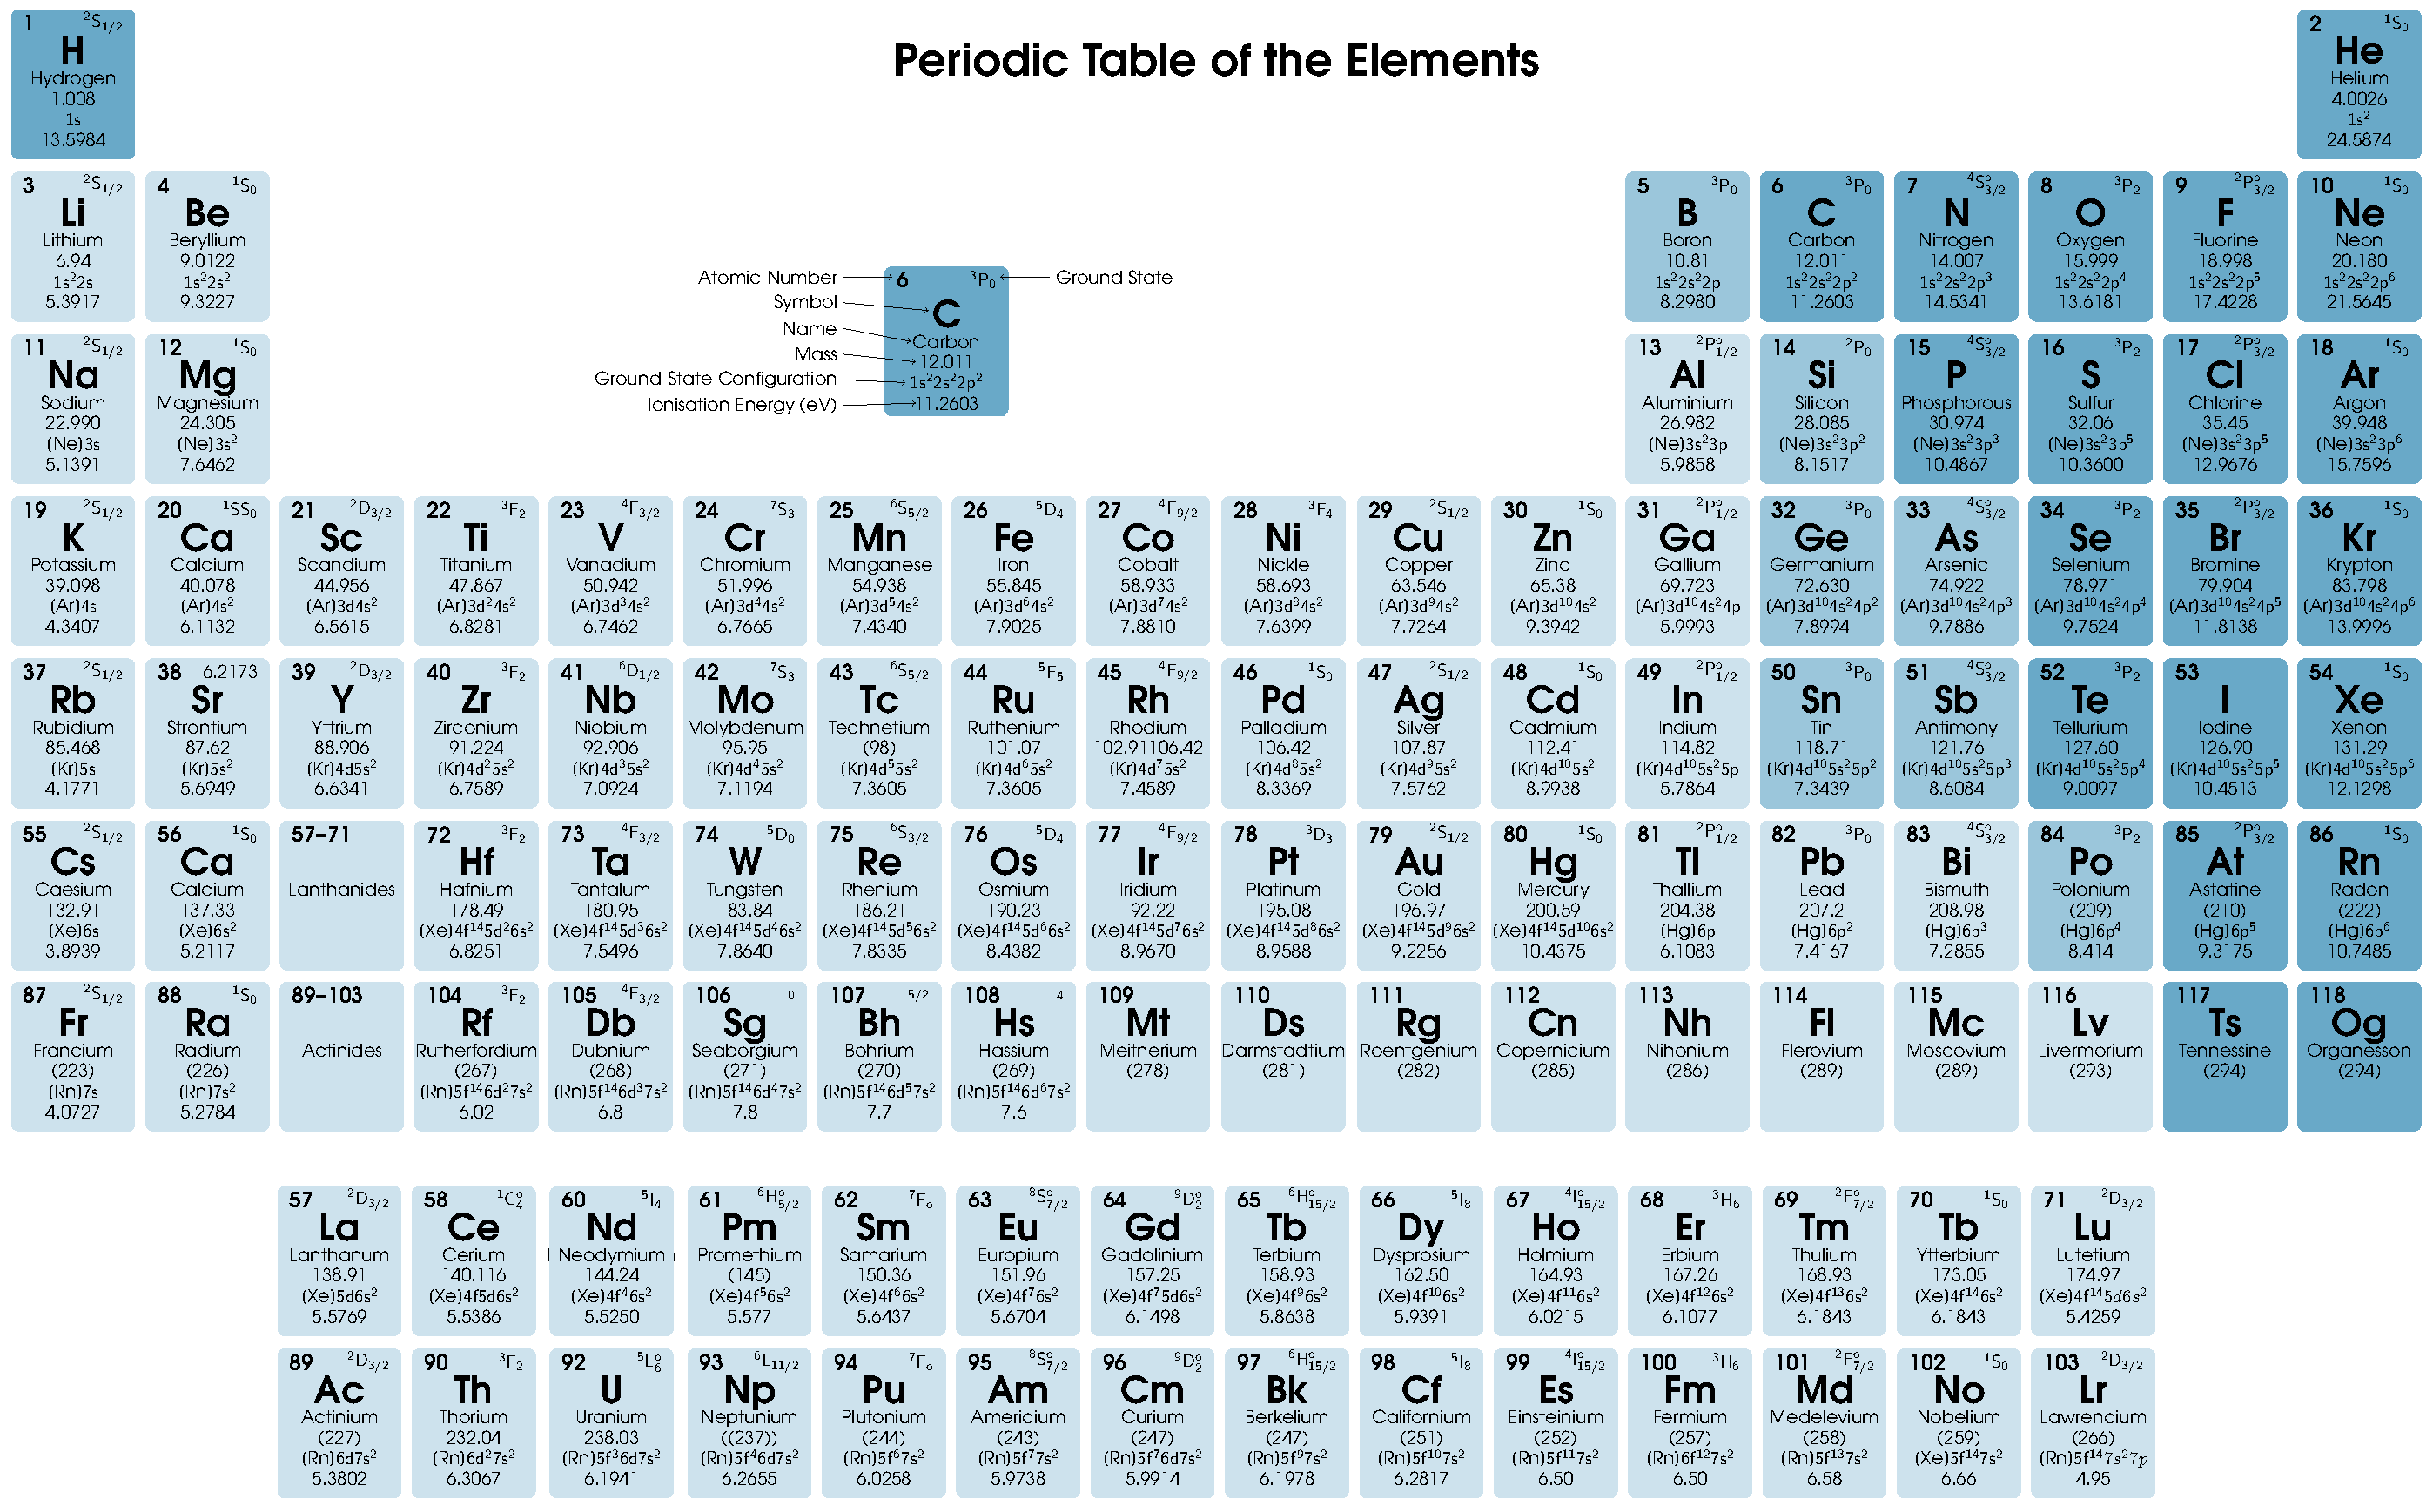
\includegraphics[height=\textwidth, angle=90]{images/periodic-table/periodic-table.pdf}
    \tikzexternaldisable
    \caption[Periodic table.]{Periodic table of the elements: \protect\tikz{\fill[highlight!20] (0, 0) circle [radius = 0.1];} Metals; \protect\tikz{\fill[highlight!40] (0, 0) circle [radius = 0.1];} Metaloids; \protect\tikz{\fill[highlight!60] (0, 0) circle [radius = 0.1];} Nonmetals.}
    \tikzexternalenable
\end{figure}
        \chapter{Integrals}\label{app:integrals}
        \section[\texorpdfstring{\(\int_0^{\infty} x^{p - 1}/(\e^{x} - 1) \dd{x}\)}{integral from 0 to infinty of x to the p-1 over e to the x - 1 dx}]{\texorpdfstring{\(\lowercase{\bm{\int_0^{\infty} x^{p - 1}/(\e^{x} - 1)} \dd{x}}\)}}{integral from 0 to infinity of x to the p-1 over e to the x - 1 dx}
        Consider the integral
        \begin{equation}
            I_p = \int_{0}^{\infty} \frac{x^3}{\e^x - 1} \dd{x}
        \end{equation}
        for \(p\) with \(\Re(p) > 1\).
        Rewriting the integrand we can identify a geometric series:
        \begin{align}
            I_p &= \int_{0}^{\infty} \e^{-x} x^{p-1} \frac{1}{1 - \e^{-x}} \dd{x}\\
            &= \int_{0}^{\infty} \e^{-x}x^{p - 1} \left[ \sum_{m=0}^{\infty} (\e^{-x})^m \right] \dd{x}\\
            &= \int_{0}^{\infty} x^{p-1} \sum_{m=0}^{\infty} \e^{-(m + 1)x}.
        \end{align}
        The geometric series converges uniformly in its region of convergence, which is everywhere in this integral since \(x > 0\) and so \(\abs{\e^{-x}} < 1\).
        This means we can swap the sum and integral to get
        \begin{equation}
            I_p = \sum_{m=0}^{\infty} \int_{0}^{\infty} \e^{-(m + 1)x} x^{p - 1} \dd{x}.
        \end{equation}
        We can re-index the sum to \(n = m + 1\) to give
        \begin{equation}
            I_p = \sum_{n=1}^{\infty} \int_{0}^{\infty} \e^{-nx}x^{p - 1} \dd{x}.
        \end{equation}
        We now make the substitution \(u = nx\), so \(\dl{u} = n\dd{x}\).
        This gives
        \begin{align}
            I_p &= \sum_{n=1}^{\infty} \frac{1}{n} \int_{0}^{\infty} \e^{-u} \frac{u^{p-1}}{n^{p-1}} \dd{u}\\
            &= \sum_{n=1}^{\infty} \frac{1}{n^p} \int_{0}^{\infty} \e^{-u}u^{p - 1} \dd{u}\\
            &= \zeta(p) \Gamma(p)
        \end{align}
        where we have identified the \defineindex{Riemann zeta function} and \defineindex{gamma function}
        \begin{equation}
            \zeta(p) \coloneqq \sum_{n=1}^{\infty} \frac{1}{n^p}, \qqand \Gamma(p) \coloneqq \int_{0}^{\infty} \e^{-u}u^{p - 1} \dd{u}.
        \end{equation}
        Both of these can be evaluated exactly only at certain values.
        One of the values we care about is \(p = 4\), for which we have \(\zeta(4) = \pi^4/90\) and \(\Gamma(4) = (4 - 1)! = 6\).
        This gives
        \begin{equation}
            I_4 = \int_{0}^{\infty} \frac{x^3}{\e^x - 1} \dd{x} = \zeta(4)\Gamma(4) = \frac{\pi^4}{15}.
        \end{equation}
    \end{appendices}

    \backmatter
    \begin{thebibliography}{9}
        \bibitem{Inductiveload2008} Inductiveload, \textit{Brillouin Zone (1st, FCC)}, \url{https://commons.wikimedia.org/wiki/File:Brillouin_Zone_(1st,_FCC).svg}, 05/05/2008 (accessed 01/11/2021).
        \bibitem{phonondispersionrelation} \url{www.phonon.fc.pl} (no longer available) via course notes (accessed 01/11/2021).
    \end{thebibliography}
    \renewcommand{\glossaryname}{Acronyms}
    \printglossary[acronym]
    \printindex
\end{document}
